%\documentclass[11pt]{scrbook} % use larger type; default would be 10pt

% WITH BLEED
% US Trade => 6x9, with a 0.125 bleed
% Adjust images size and gutter so tabs bleed by .125
% See https://www.createspace.com/Products/Book/InteriorPDF.jsp

%\documentclass[paper=6.14in:9.21in,pagesize=pdftex,11pt,twoside,openright]{scrbook}

\documentclass[paper=7in:9in,pagesize=pdftex,11pt,twoside,openright]{scrbook}


%openright
% Paper width
% W = 7.125in (7+0.125 --- bleed)
% Paper height
% H = 9.25in (9+2*.125 --- bleed)
% Paper gutter
% BCOR = 0.375in (0.5+0.5-0.625 --- margin with bleed)
% Margin (0.5in imposed on lulu, recommended on createspace)
% m = 0.625in (0.5+0.125 --- bleed)
% Text height
% h = H - 2m = 8in
% Text width
% w = W - 2m - BCOR = 4.5in
\areaset[0.375in]{5.5in}{8in}
\usepackage[utf8]{inputenc} % set input encoding (not needed with XeLaTeX)

% \usepackage{subfig} % make it possible to include more than one captioned figure/table in a single float
% Subfigure is deprecated
% Subfig is not compatible with hyperref
\usepackage{subcaption}
\captionsetup{format=plain,indention=.4cm,labelformat=simple, labelfont = sl, labelsep=period, font=small}
% \captionsetup[sub]{labelformat=simple,labelsep=period, font=small}

%%% Examples of Article customizations
% These packages are optional, depending whether you want the features they provide.
% See the LaTeX Companion or other references for full information.

\usepackage{mitpress}
\usepackage[usenames, dvipsnames, table]{xcolor}

\usepackage[framemethod=TikZ]{mdframed}
\mdfsetup{skipbelow=2pt, backgroundcolor=gray!8, linecolor=black!40}

\usepackage[top=1in, bottom=1in, left=1in, right=1in]{geometry}

\usepackage{graphicx} % support the \includegraphics command and options
%\usepackage{wrapfig}

% \usepackage[parfill]{parskip} % Activate to begin paragraphs with an empty line rather than an indent

%%% PACKAGES
\usepackage{booktabs} % for much better looking tables
\usepackage{array} % for better arrays (eg matrices) in maths
\usepackage{paralist} % very flexible & customisable lists (eg. enumerate/itemize, etc.)
\usepackage{verbatim} % adds environment for commenting out blocks of text & for better verbatim
% These packages are all incorporated in the memoir class to one degree or another...
\usepackage{amsmath}
\usepackage{mathtools}
\usepackage{amsfonts}
\usepackage{amssymb}
\usepackage{hyperref}
\usepackage{harvard}
\usepackage{fancyvrb}
\usepackage{marginnote}
\usepackage[capitalize, noabbrev]{cleveref} % Used to improve refernces
\usepackage{tikz}
\usetikzlibrary{automata, positioning}
\usepackage{tikz-qtree}
\usepackage{forest}
\usepackage{enumitem}
\usepackage[xindy]{imakeidx}

\colorlet{mylinkcolor}{BrickRed}
\colorlet{mycitecolor}{PineGreen}
\colorlet{myurlcolor}{NavyBlue}

\hypersetup{
  linkcolor  = mylinkcolor,
  citecolor  = mycitecolor,
  urlcolor   = myurlcolor,
  colorlinks = true,
}

\usepackage{makeidx}
\usepackage{idxlayout}

\usepackage{import}
\usepackage{xifthen}
\usepackage{pdfpages}
\usepackage{transparent}

% \let\comment=\relax
\usepackage[markup=bfit, deletedmarkup=sout, authormarkup=superscript, commandnameprefix=ifneeded]{changes}
\definechangesauthor[name={ar}, color=teal]{AR}
\definechangesauthor[name={nc}, color=green]{NC}
\definechangesauthor[name={bh}, color=blue]{BH}
\definechangesauthor[name={td}, color= red]{TODO}

\newcommand{\ar}[1]{\added[id=AR  ]{#1}}
\newcommand{\nc}[1]{\added[id=NC  ]{#1}}
\newcommand{\bh}[1]{\added[id=BH  ]{#1}}
\newcommand{\td}[1]{\added[id=TODO]{#1}}
%\newcommand{\cref}[1]{Section \ref{#1}}

\newcommand{\hjb}[1]{{\color{red}#1}}


% fixing a scrbook error when compiling the citations
\DeclareOldFontCommand{\bf}{\normalfont\bfseries}{\mathbf}

\DeclareUnicodeCharacter{00A0}{ }

%%% HEADERS & FOOTERS
%\usepackage{fancyhdr} % This should be set AFTER setting up the page geometry
%\pagestyle{fancy} % options: empty , plain , fancy
%\renewcommand{\headrulewidth}{0pt} % customise the layout...
%\lhead{}\chead{}\rhead{}
%\lfoot{}\cfoot{\thepage}\rfoot{}

%%% APPEARANCE OF SECTIONS
\usepackage[up,md,sf]{titlesec}

%%% APPEARANCE OF ToC (Table of Content)
%\usepackage[nottoc,notlof,notlot]{tocbibind} % Put the bibliography in the ToC
%\usepackage[titles,subfigure]{tocloft} % Alter the style of the Table of Contents

\newcommand{\screencast}[2]{
  \marginnote{\href{#1}{\includegraphics[trim=5 20 0 0, clip, width=1.8cm]{figs/youtube/#2}}}}


%%% END Article customizations

%%% The ``real'' document content comes below...
\makeindex

%\title{Introduction to Autonomous Robots}
%\author{Nikolaus Correll}
%\date{} % Activate to display a given date or no date (if empty),
         % otherwise the current date is printed

\allowdisplaybreaks

\begin{document}
%\maketitle


\thispagestyle{empty}
\begin{flushleft}
Nikolaus Correll, Bradley Hayes,\\ Christoffer Heckman, and Alessandro Roncone \\~\\
Introduction to Autonomous Robots:\\ Mechanisms, Sensors, Actuators, and Algorithms\\~\\
v2.0, \today\\
%Magellan Scientific\\
%ISBN-13: 978-1493773077
%ISBN-13: 978-0692700877
\end{flushleft}

\vfill

\begin{figure}[!h]

\includegraphics[width=1.2in]{figs/by-nc-nd}
\end{figure}

Copyright in this monograph has been licensed exclusively to The MIT Press, \url{http://mitpress.mit.edu}, which will be releasing the final version to the public in 2022. All inquiries regarding rights should be addressed to The MIT Press, Rights and Permissions Department.
Source code of this book is licensed under a Creative Commons Attribution-NonCommercial-NoDerivatives 4.0 International (CC BY-NC-ND 4.0). You are free to share, i.e., copy, distribute and transmit sources under the following conditions: you must attribute the work to its main author, you may not use this work for commercial purposes, and if you remix or modify this work you may not distribute the modified material. For more information, please consult \url{https://creativecommons.org/licenses/by-nc-nd/4.0/}.


\cleardoublepage
\thispagestyle{empty}
\topskip0pt
\vspace*{\fill}
\begin{center}
For Arthur, Tatiana, Benedict and Silvester\\
David
\\
Leonardo and Lily\\
future robot users\\
\end{center}
\vspace*{\fill}

\tableofcontents

\chapter*{Preface}

This book provides an algorithmic perspective to autonomous robotics to students with a sophomore-level of linear algebra and probability theory. Robotics is an emerging field at the intersection of mechanical engineering, electrical engineering, and computer science. With computers becoming more powerful, making robots smart is getting more and more into the focus of attention and robotics research most challenging frontier. While there is a large number of textbooks on the mechanics and dynamics of robots available to sophomore-level undergraduates, books that provide a broad algorithmic perspective are mostly limited to the graduate level. This book has therefore been developed not to create ``yet another textbook, but better than the others'', but to allow us to teach robotics to the 3rd and 4th year undergraduates at the Department of Computer Science at the University of Colorado.

Although falling under the umbrella of ``Artificial Intelligence'', standard AI techniques are not sufficient to tackle problems that involve uncertainty, such as a robot's interaction in the real world. This book uses simple trigonometry to develop the kinematic equations of manipulators and mobile robots, then introduces path planning, sensing, and lastly uncertainty. The robot localization problem is introduced by formally defining error propagation, which leads to Markov localization, Particle filtering and finally the Extended Kalman Filter, and Simultaneous Localization and Mapping.

Instead of focusing on state-of-the-art solutions to a particular sub-problem, emphasis of the book is on a progressive step-by-step development concepts through recurrent examples that capture the essence of a problem. The described solutions might not necessarily be the best, however they are easy to comprehend and widely used in the community. For example, odometry and line-fitting are used to explain forward kinematics and least-squares solutions, respectively, and later serve as motivating examples for error propagation and the Kalman filter in a localization context.

Notably, the book is explicitly robot-agnostic, reflecting the timeliness of fundamental concepts. Rather, a series of possible project-based curricula are described in an Appendix and available online, ranging from a maze-solving competition that can be realized with most camera-equipped differential-wheel robots to manipulation experiments with a robotic arm, all of which can be entirely conducted in simulation to teach most of the core concepts.

After multiple years of development and distribution mainly via Github, this new edition of the book has been co-authored by my colleagues in the Computer Science department, Bradley Hayes, Christoffer Heckman, and Alessandro Roncone, each having thaught multiple iterations of our ``Introduction to Robotics'' and ``Advanced Robotics'' courses as well as special topics courses that pertain to their sub-fields of robotics research. They are adding not only tremendous technical depth, but also years of experience on how certain subjects should be taught to remain engaging and exciting.

This book is released under a Creative Commons CC BY-NC-ND 4.0 International license, which allows anyone to copy and share its source code. However, neither the compiled version nor the code shall be used to create derivatives for commercial purposes. We have chosen this format as it seems to maintain the best trade-off between a freely available textbook resource that others may contribute to and maintaining a consistent curriculum that others can refer to. We are incredibly grateful to MIT Press and our editor Elizabeth Swayne to support this forward-looking model.

Writing this book would not have been possible without the excellent work of others before us, most notably ``Introduction to Robotics: Mechanics and Control'' by John Craig and ``Introduction to Autonomous Mobile Robots'' by Roland Siegwart, Illah Nourbakhsh and Davide Scaramuzza, and innumerable other books and websites from which I learned and borrowed examples and notation. We are also grateful to Brian Amberg, Aaron Becker, Bachir El-Kadir,  James Grime, Michael Sambol, Cyrill Stachniss, Subh83, Ethan Tiran-Thompson who made lecture video snippets and animations available online, and which are referenced throughout the book using QR codes.

I would like to acknowledge Mike Miles and Harel Biggie, graduate students in the authors' shared laboratory at the University of Colorado Boulder, for their careful reading and contributions. Finally, I would also like to acknowledge Github users AlWiVo, beardicus, mguida22, aokeson, as1ndu, apnorton, JohnAllen, jmodares, countsoduku, choffmann, and chrstphrdlz for their pull requests and comments as well as Haluk Bayram. Your interest and motivation in this project has been one of our biggest rewards.

\begin{flushright}
Nikolaus Correll\\
Boulder, Colorado, \today
\end{flushright}

\chapter{Introduction}\label{chap:introduction}
Robotics celebrated its 60th birthday in 2021, dating back to the first commercial robot in 1961 (the Unimate). In a ``Tonight Show'' at the time, this robot did amazing things: it opened a bottle of beer, poured it, put a golf ball into a hole, and even conducted an orchestra. This robot did all what we expect a good robot to do: it is dexterous, it is accurate, and even creative. Since this robot's appearance on the Tonight show, more than 60 years have passed --- so how incredible must be the capabilities of today's robots and what must they be able to do?

Interestingly, we just recently learned doing all the things demonstrated by Unimate autonomously. Unimate indeed did what was shown on TV, but all motions have been preprogrammed and the environment has been carefully staged.  Only the advent of cheap and powerful sensors and computation has recently enabled robots to detect an object by themselves, plan motions to it and grasp it. Yet, robotics is still far away from doing these tasks with human-like performance.

This book introduces you to the computational fundamentals of autonomous robots. Robots are \emph{autonomous} when they make decisions in response to their environment vs.\ simply following a pre-programmed set of motions. They achieve this using techniques from signal processing, control theory, and artificial intelligence, among others. These techniques are tightly intertwined  with the mechanics, the sensors, and the actuators of the robot. Designing a robot therefore requires a deep understanding of both algorithms and its interfaces to the physical world.

The goals of this introductory chapter are to introduce the kind of problems roboticists deal with and how they solve it.

\section{Intelligence and embodiment}
Our notion of ``intelligent behavior'' is strongly biased by our understanding of the brain and how computers work: intelligence is located in our heads. In fact, however, a lot of behavior that looks intelligent can be achieved by very simple means. For example, mechanical wind-up toys can avoid falling off an edge simply by using a fly-wheel that rotates at a right angle to their direction of motion and a caster wheel. Once the caster wheel loses contact with the ground---that is the robot has reached the edge---the fly-wheel kicks in and pulls the robot to the right (Figure~\ref{fig:winduptoy}).

\begin{figure}
    \centering
    % \includegraphics[width=\textwidth]{figs/winduptoysketch.png}
    \def\svgwidth{\textwidth}
    \import{./figs/}{winduptoy.pdf_tex}
    \caption{A wind-up toy that does not fall off the table using purely mechanical control. A fly-wheel that turns orthogonal to the robot's motion induces a right turn as soon as it hits the ground once the front caster wheel goes off the edge.}
    \label{fig:winduptoy}
\end{figure}

A robot vacuum cleaner might solve the same problem very differently: it employs infrared sensors that are pointed downwards to detect edges such as stairs and then issues a command to make an avoiding turn. Once electronics are on-board, this is a much more efficient, albeit much more complex, approach.

Whereas the above examples provide different approaches to implement intelligent behaviors, similar trade-offs exist for robotic planning. For example, ants can find the shortest path between their nest and a food source by simply choosing the trail that already has more pheromones, the chemicals ants communicate with, on it. As shorter paths have ants not only moving faster towards the food, but also returning faster, their pheromone trails build up quicker (Figure~\ref{fig:ants}). But ants are not stuck to this solution. Every now and then, ants give the longer path another shot, eventually finding new food sources. What looks like intelligent behavior at the swarm level, is essentially achieved by a pheromone sensor that occasionally fails. A modern industrial robot would solve the problem completely differently: it would first acquire some representation of the environment in the form of a map populated with obstacles, and then plan a path using an algorithm.

\begin{figure}
    \centering
    % 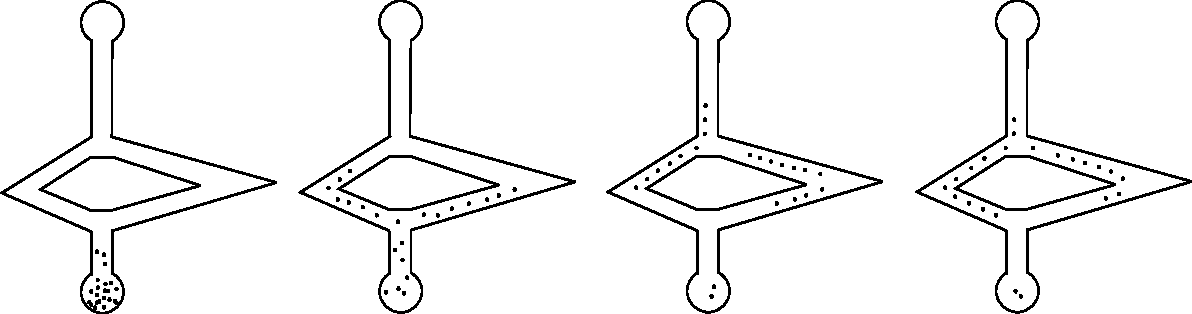
\includegraphics[width=\textwidth]{figs/ants.png}
    \def\svgwidth{\textwidth}
    \import{./figs/}{ants.pdf_tex}
    \caption{Ants finding the shortest path from their nest (bottom) to a food source (top). From left to right: The ants initially have equal preference for the left and the right branch, both going back and forth. As ants return faster on the shorter branch there will be more pheromones present on the short branch once a new ant arrives from the nest.}
    \label{fig:ants}
\end{figure}

Which solution to achieve a certain desired behavior is best depends on the resources that are available to the designer. We will now study a more elaborate problem for which many, more or less efficient, solutions exist.

\section{A roboticists' problem}
Imagine the following scenario. You are a robot in a maze-like environment such as a cluttered warehouse, hospital or office building. There is a chest full of gold coins hidden somewhere inside. Unfortunately, you don't have a map of the maze. In case you find the chest, you may only take a couple of coins at a time, and bring them to the exit door where your car is parked.

\begin{mdframed}
Think about a strategy that will allow you to harvest as many coins in the shortest time as possible. Think about the cognitive and perception capabilities you would make use of. Now discuss alternative strategies, if you would not have these capabilities, i.e., what if you were blind, had no memory?
\end{mdframed}

These are exactly the same problems a robot would have. A robot is a mobile machine that has sensors and computation, which allows it to reason about its environment. Current robots are far from the capabilities that humans have, therefore it makes a lot of sense to think about what strategies \emph{you} would employ to solve a problem, if you were lacking important perception or computational capabilities.

Before we move forward to discuss potential strategies for robots with impeded sensory systems, let's quickly consider an optimal strategy. You will need to explore the maze without entering any branch twice. You can use a technique known as \emph{depth-first search} to do this, but will need to be able to not only map the environment, but also localize in the environment, e.g., by recognizing places and dead-reckoning on the map. Once you have found the gold, you will need to plan the shortest path back to the exit, which you can then use to go back and forth until all the gold is harvested.

\section{An example of autonomous mobile robotics: Ratslife}\label{sec:ratslife}
Ratslife is a miniature robot maze competition developed by Olivier Michel from Cyberbotics S.A., which exemplifies a broad range of topics covered in this book. The Ratslife environment can easily be created from LEGO bricks, card board or wood and the game can be played with any two mobile robots, preferably ones with the ability to identify markers in the environment. These include simple differential-wheel educational platforms with onboard cameras or even a smart-phone driven robot. Figure~\ref{fig:ratslife} shows a simple sample environment that can be constructed from craft materials and can be used to teach the practical aspects of mobile robots for competitions.


\begin{figure}
    \centering
    % 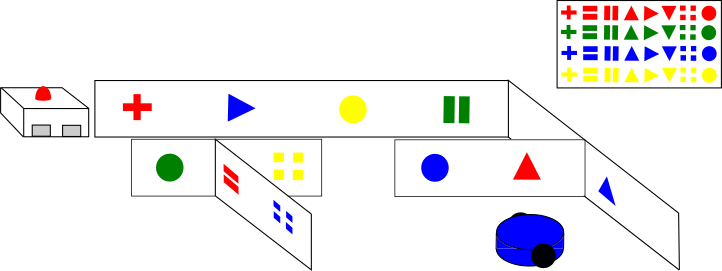
\includegraphics[width=\textwidth]{figs/ratslife.png}
    \def\svgwidth{\textwidth}
    \import{./figs/}{ratslife.pdf_tex}
    \caption{A simple maze made from cardboard, wood or Lego bricks with one or more charging stations. Locations in the maze are marked with unique markers that can be recognized by a simple robot.}
    \label{fig:ratslife}
\end{figure}

In RatsLife, two miniature robots  compete on searching for four ``feeders'' that are hidden in  a maze. Once a robot reaches a feeder, it receives ``energy'' to go on for another 60s, and the feeder becomes temporarily unavailable. After a short while, the feeder becomes available again. The feeders can be either controlled by a referee who also takes care of time-keeping or constructed as part of a simple curriculum on electronics or mechatronics.

It should be clear by now, how YOU would solve these tasks using your abilities, and you should have also thought about fall-back strategies in case some of your sensors are unavailable. Here are some possible algorithms for a robot, ordered after the capabilities that it provides:
\begin{itemize}
\item Imagine you have a robot that can only drive (actuation) and bounce off a wall. The resulting random walk will eventually let the robot reach a feeder. As the allowed time to do so is limited, it is likely that the robot's energy will soon deplete.
\item Now imagine a robot that has a sensor that gives it the ability to estimate its distance from a wall. This could be a whisker, an infrared distance sensor, an ultra-sound distance sensor, or a laser range finder. The robot could now use this sensor to keep following a wall to its right. Using this strategy for solving the maze, it will eventually explore the entire maze except for islands inside of it.
\item Finally, think about a robot that could identify simple patterns using vision, has distance sensors to avoid walls, and an ``odometer'' to keep track of its wheel rotations. Using these capabilities, a potential winning strategy would be to explore the environment, identify markers in the environment using vision and use them to create a map of all feeder locations, calculate the shortest path from feeder to feeder and keep going back and forth between them. Strategy-wise, it might make sense to wait just in front of the feeder and approach it only shortly before the robot runs out of power.
\end{itemize}

\section{Challenges of Mobile Autonomous Robots}

Being able to stitch sensor information together to map the environment just by counting your own steps and orienting yourself by using distinct features of the environment is known as Simultaneous Localization and Mapping (SLAM). The key challenge here is that the length of the steps you take are uncertain (a wheeled robot might slip or have slightly differently sized wheels) and it is not possible to recognize places with 100\% accuracy (even humans can have trouble with this). In order to be able to implement something like the last algorithm on a real robot, we will therefore need to understand

\begin{itemize}
\item How does a robot move? How does rotation of its wheels affect its position and speed in the world?
\item How do we have to control the wheel-speed in order to reach a desired position?
\item What sensors exist for a robot to perceive its own status and its environment?
\item How can we extract structured information from a vast amount of sensor data?
\item How can we localize in the world?
\item How can error be represented and how can we reason in the face of uncertainty?
\end{itemize}

In order to answer these questions, we will rely on trigonometry, linear algebra, and probability theory. Specific concepts that will be used throughout this book are basic trigonometry, matrix notation, Bayes' formula, and the concept of probability distributions. You will see that robotics is a great vehicle to add meaning to these concepts!


\section{Challenges of Autonomous Manipulation}
Think about the last time you worked with your hands. This includes typing on your keyboard, writing on a piece of paper, sewing a button onto a shirt, and using a hammer or a screwdriver. You will notice that these activities require a wide range of dexterity, that is the ability to manipulate objects with precision, a wide range of forces, and a wide range of sensorial capabilities. You will also notice that some tasks go beyond your natural capabilities, such as putting yarn through a hole in fabric, turning a screw, or driving a nail into a piece of wood, but can be easily solved with the right tool.

So far, robotic hands are far from reaching the dexterity of a human hand. Yet, with the right tool (called ``end-effector'' in robotics speech) \index{End-effector} some tasks can be solved even better, that is faster and more precisely, than by humans. As for solving a mobile robotics problem, manipulation problems require you to think about the right mix of reasoning and mechanism design. For example, grasping tiny parts might be impossible with tweezers, but really easy when using a sucking mechanism. Or, picking up a test tube that is hardly visible with the robots' sensors can be picked up almost blindly when using a funnel-like mechanism at your end-effector. Unfortunately, these tricks will most likely limit the versatility of your robot, requiring you to think about the problem and the users's need as a whole.

%\section{The first industrial robot ``Unimate"}
%Since the introduction of the first industrial robot ``Unimate'' in 1961, the robotics industry classically consists of static manipulators that perform repetitive tasks such as welding or part placement, as well as of remote controlled machines for exploring hazardous areas. Recent advances in sensor technology and artificial intelligence are quickly enabling a new kind of robotic system: robots that can make autonomous decisions. The most prominent example of this class of robots is iRobot's ``Roomba'' vacuum cleaner that was introduced in 2002 and that uses a variation of algorithm \#1 above to solve the floor cleaning problem due to the lack of sophisticated sensors and computation. More recently, SLAM has found its ways into cars, university teams winning the DARPA Grand Challenge, Google's cars logging more than 140,000 miles, and Volkswagen presenting the first assisted driving system in 2011. Similarly, KIVA systems  successfully distributes mobile robots for automatic warehouses. These robots are still remote controlled and operate in constrained environments that provide them the ability to localize and reason on a simplified representation of the world - all items in the KIVA world are living on a grid. Novel sensors such as the xBox Kinect that provide 3D depth measurements at unprecedented low cost, increasingly capable and cheap computers, and a better understanding on how to reason about uncertainty will enable a large number of applications raising from autonomous warehouse helpers, home and elderly care, robotic toys and many other gimmicks straight from the Jetsons very soon.



\section*{Take-home lessons}
\begin{itemize}
\item The best solution to a problem is a function of the available sensing, actuation, computation and communication abilities of the available platform. Usually, there exist trade-offs that allow you to solve a problem using a minimal set of resources but compromise performance characteristics such as speed, accuracy or reliability.
\item Robotics problems are different from many problems in pure Artificial Intelligence, particularly those that do not deal with unreliable sensing or actuation.
\item The unreliability of sensors, actuators and communication links require a probabilistic notion of the system and the ability to reason with uncertainty.
\end{itemize}

\section*{Exercises}\small
\begin{enumerate}
\item What kind of sensors do you need to solve the ``Ratslife'' game? Think both about trivial and close-to-optimal approaches.
\item What devices in your home could be considered robots? Why and why not?
\item Is a mechanical clock a robot? Why or why not?
\item Which industries have been recently revolutionized by robotics? Into which industries were robots introduced first? Which industries are currently being transformed?
\item What sensors are you using when you grasp an object? Enumerate them all. Which ones are absolutely necessary and which one could you live without?
\item Think about robots vacuuming your floor or mowing your lawn. Do they use any planning? Is planning necessary? Why or why not?
\item What kind of sensors would you need in a car that drives completely autonomously? Think first about the kind of information that the car needs to be aware of and then discuss possible sensors that could capture this information.
\item Implement a simple line-following using a robot of your choice. How does the thickness of the line affect the sensor placement on the robot? How does its curvature affect the robot's maximum speed?
\item Implement a maze solving algorithm that uses simple wall-following using a robot of your choice. How does the sensor geometry affect the robot's performance? What are the parameters that you find yourself tuning?
\end{enumerate}\normalsize

%Robotics celebrated its 50th birthday in 2011, dating back to the first commercial robot in 1961 (the Unimate). In a ``Tonight show'' from the time, this robot did amazing things: its opening a bottle of beer, pouring it, putting a golf ball into the hole, and even conducting an orchestra. This robot does all what we expect a good robot to do: its dexterous, its accurate, and even creative. Since this robots appearance on the Tonight show more than 50 years have passed --- so how incredible must be the capabilities of today's robots and what must they be able to do?
%
%Interestingly, we just recently learned doing all the things demonstrated by Unimate autonomously. Unimate indeed did what was shown on TV, but all motions have been pre-programmed and the environment has been carefully staged.  Only the advent of cheap and powerful sensors and computation has recently enabled robots to detect an object by themselves, plan motions to it and grasp it. Yet, robotics is still far away from doing these tasks with human-like performance. Environments still need to be heavily staged for a robot to operate, and some objects are easier to work with than others. For example, ``Rollin' Justin'' is demonstrating skills very similar to those shown by the Unimate, but is able to perceive and reason about its environment:
%
%This works as follows: the robot perceives its environment with a sensor that generates 3D range data, such as stereo-vision, a sweeping laser scanner or an xbox Kinect. The robot creates a 3D representation of its environment that is relative to its own coordinate system. The robot now plans its motion using this 3D representation. This can be seen in the inset to the top right when the robot is manipulating items on the table. Detecting objects in the environment, matching them to their 3D model, and finding feasible grasp points are still major research challenges.
%
%The ``sense-plan-act'' paradigm, that is obtaining a 3D model of the world, planning therein, and consequently executing actions is not the final solution, however. Do humans really do this when performing complex manipulations? Rather not. Instead, we are relying on vision feedback or the sense of touch when performing a grasp. (Try to grasp an object after putting your hand on an ice block, temporarily impeding your sense of touch.)
%
%This class builds up on ``Introduction to Robotics'' and introduces current solutions to these problems. We will learn advanced concepts in robotic kinematics, such as car-like steering and inverse kinematics of high-DOF manipulators, feature recognition, RGB-D perception, visual servoing and SLAM. We will also learn to use state-of-the-art tools that allow you to model, visualize and control your robot. You will work with a 7-DOF manipulator arm both in simulation and using real hardware. The development environment consists of Ubuntu Linux, ROS and OpenCV that are available as VirtualBox. The real manipulator arm is available for experimentation in the lab. We will perform laboratory experiments - that can be mostly prepared and executed in simulation - that will introduce the tools and methods we are using and guide you toward an independent project.
%
%The class consists of homework assignments (experiments) and a team project. The final deliverable for the team project is a 3 page (5 pages) for undergraduates (graduate students). Your team project needs to articulate a hypothesis (what do you want to show?) that is validated experimentally on physical hardware. In order to prepare you for this, each laboratory exercise will require analysis of experimental data rather than submission of code.


\part{Mechanisms}
%!TEX root = ../book.tex
\chapter{Locomotion, manipulation and their representations}\label{chap:locomotion}

Autonomous robots are systems that sense, compute, communicate, and actuate. Actuation, the focus of this chapter, is the ability of the robot to move and to manipulate the world. Specifically, we differentiate between locomotion\index{Locomotion} as the robot's ability to move itself and manipulation\index{Manipulation} as the robot's ability to move objects in the environment. Both activities are closely related: during locomotion the robot uses its motors to exert forces on its environment (ground, water, or air) to move itself; during manipulation it uses motors to exert forces on objects to move them relative to the rest of the environment. This might not even require different motors. Insects are good examples for this: they can use their six legs not only for locomotion, but also for picking up and manipulating objects. In short, the goals of this chapter are to:
\begin{itemize}
\item Introduce the concepts of locomotion, manipulation and their duality,
\item Explain static vs.\ dynamic stability,
\item Introduce the concept of ``Degree of Freedom'' (DoF),
\item introduce coordinate systems and their transformations.
\end{itemize}

\section{Locomotion and manipulation examples}

Locomotion includes very different concepts of motion, including rolling, walking, running, jumping, sliding (undulatory locomotion), crawling, climbing, swimming, and flying. The mechanisms that might achieve these feats could be drastically different in terms of energy consumption, kinematics, stability, and other capabilities required by the robot that implements them. Furthermore, the above definitions are loose and ambiguous: for example, ``swimming'' can be performed using many different forms of propulsion. Similarly, a sliding motion on the ground might work well for swimming too with only few modifications.

The way in which the individual parts of a robot can move with respect to each other and the environment is called the \textsl{kinematics}\index{Kinematics} of the robot. Kinematics (which will be discussed in detail in \cref{chap:kinematics}) are only concerned with the position and speed (first derivative of position) of those parts; depending on the application, one may want to use a deeper level of abstraction called \textsl{dynamics}\index{Dynamics}, which is concerned with quantities such as acceleration (second derivative of position) and jerk (third derivative of position).

Commercially, the most widespread form of locomotion is rolling. This is partially due to the fact that rolling provides by far the most efficient energy to speed ratio (see \cref{fig:todd}), making the invention of the wheel one of the greatest technological breakthroughs in history. It also is a widely implemented form of locomotion, e.g.\ with cars and bicycles. Consequently, humans have modified their environment to have as many smooth surfaces as possible---e.g. roads, warehouses, and residential floors.
%
In contrast, evolution has not equipped any animal with wheel-like actuators because of their poor performance in natural environments such as an unmown meadow, a forest floor, a mountains or a cave; consequently, wheeled robots perform poorly in such environments, whereas legged robots can shine.

\begin{figure}
    \centering
    \includegraphics[width=0.8\textwidth]{figs/todd85.png}
    \caption{Power consumption vs.\ speed for various means of locomotion. From \protect\citeasnoun{todd1985walking}.}
    \label{fig:todd}
\end{figure}


\begin{mdframed}Can you find examples of robots from the above categories (legged vs wheeled robots)? Identify the different types of actuators that are used in them.
\end{mdframed}

Most mechanisms capable of locomotion can also be used for manipulation with only minor modifications. Most industrial manipulators consist of a chain of rotary (or revolute) actuators that are connected by rigid links. In general, they are equipped with six or more independently rotating axes---we will see why further down below. In addition, modern industrial manipulators have the ability to not only control the position of each of its joints, but to also control the torque at each individual joint; this capability allows control over the \textsl{compliance}\index{Compliance} of a robot, which in a mechanical sense is the inverse of stiffness. Finally, for dexterous manipulation a robot does not only need an arm, but also a gripper or hand. Grasping is a hard problem on its own and is therefore treated in its own chapter (\cref{chap:grasping}).


Regardless of whether the robot is rolling or walking, the dominant actuator type is rotational. Another type of mechanism is the \emph{prismatic} or \emph{linear} joint (see Figure \ref{fig:prismaticjointkinematics} for example) that allows the robot to extend and contract a link. This type of joints are usually combined with rotating joints and allow, for example, a robot arm to move up and down, or a robotic walker to extend or retract its leg. 

%This lecture focuses on the kinematics of simple mechanisms. Understanding the duality between locomotion and manipulation is important, however, to better introduce (and understand) concepts such as reference frames and forward kinematics.

\section{Static and dynamic stability}\label{sec:stability}

A fundamental difference between locomotion mechanisms is whether they are statically or dynamically stable\index{Static stability}\index{Dynamic Stability}. A statically stable mechanism will not fall even when not actuated (\cref{fig:stability}, left). A dynamically stable robot instead requires constant actuation to prevent it from falling. Technically, stability requires the robot to keep its center of mass to fall within the polygon spanned by its ground-contact points. For example, a quadrupedal robot's feet span a rectangle. Once such a robot lifts one of its feet, this rectangle becomes a triangle. If the projection of the center of mass of the robot along the direction of gravity is outside of this triangle, the robot will fall. A dynamically stable robot can overcome this problem by changing its configuration so rapidly that a fall is prevented. An example of a purely dynamically stable robot is an inverted pendulum on a cart (\cref{fig:stability}, middle). Such a robot has no statically stable configurations and needs to keep moving all the time to keep the pendulum upright. While dynamic stability is desirable for high-speed, agile motions, robots should be designed so that they can easily switch into a statically stable configuration (\cref{fig:stability}, right).

\begin{figure}
    \centering
    % 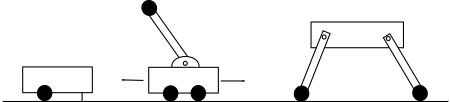
\includegraphics[width=\textwidth]{figs/stability.png}
    \def\svgwidth{\textwidth}
    \import{./figs/}{stability.pdf_tex}
    \caption{From left to right: statically stable robot; dynamically stable inverted pendulum robot; static and dynamically stable robot (depending on configuration).}
    \label{fig:stability}
\end{figure}

An example of a robot that has both statically and dynamically stable configurations is a quadruped running. Unlike walking, a running quadruped robot will always have two legs in the air and alternate between them faster than the robot may fall in either direction. Although statically stable walking is possible with only four legs, most animals (and robots) require six legs for statically stable walking and use dynamically stable gaits (such as galloping) when they have four legs. Six legs allow the animal to move three legs at a time while the three other legs maintain a stable pose.


\section{Degrees of freedom}\label{sec:dof}

The concept of \textsl{degree of freedom}\index{Degree of Freedom}, often abbreviated as DoF, is important for defining the possible positions and orientations a robot can reach. An object in the physical world can have up to six \textsl{Cartesian}\index{Cartesian}\index{Cartesian Degree of Freedom} degrees of freedom, namely forward/backward, sideways, and up/down as well as rotations around those axes. These rotations are known as pitch, yaw, and roll and are illustrated in \cref{fig:pitchyawandroll}. These Cartesian degrees of freedom are distinct from the robot's \textsl{mechanical} degrees of freedom, which correspond to the number of points of actuation for a robot (i.e., a robotic arm with five joint motors is referred to as having five mechanical degrees of freedom \textsl{in joint space}, see \cref{chap:kinematics}).
As a rule of thumb, the number of mechanical DoFs available to the user depends on the robot platform and cannot easily be changed by the user unless mechanical modifications to the robot are made; conversely, the number of Cartesian DoFs depends on the task, can be modified by the user, and varies according to what the robot needs to do.

\begin{figure}
    \centering
    % 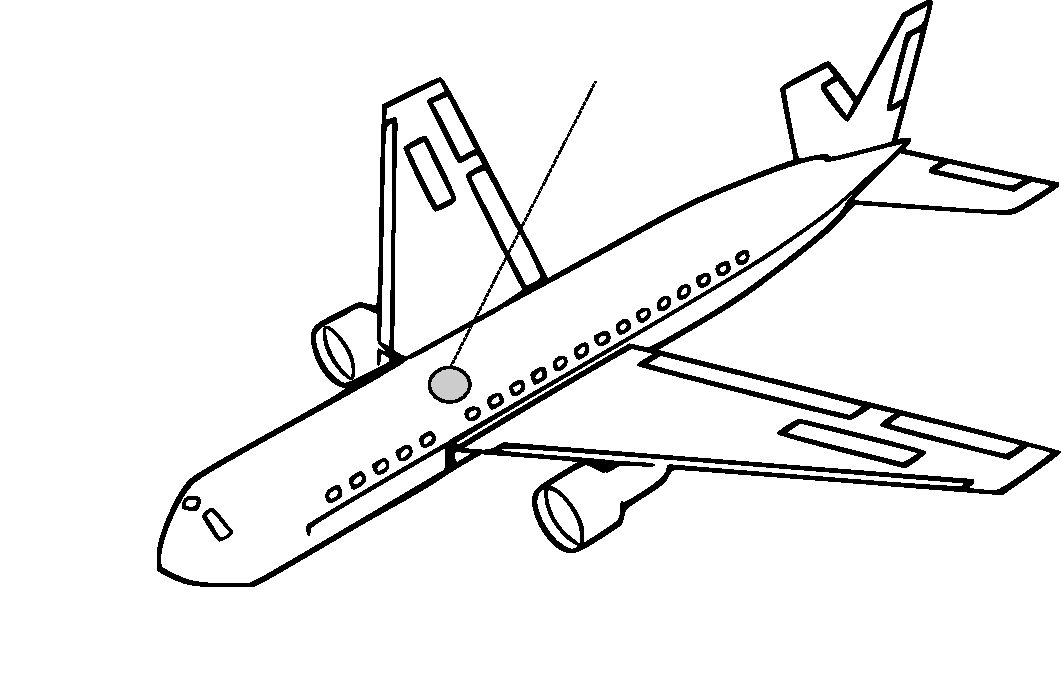
\includegraphics[width=\textwidth]{figs/pitchyawroll.png}
    \def\svgwidth{\textwidth}
    \import{./figs/}{pitchyawroll.pdf_tex}
    \caption{Pitch, yaw, and roll around the principal axis of an airplane.}
    \label{fig:pitchyawandroll}
\end{figure}

After specifying the mechanical and Cartesian DoFs for your kinematic problem, the number of Cartesian DoFs (i.e. directions) a robot can actually move in depends on the configuration of its actuators and the constraints the robot has with the environment. These relationships are not always intuitive and require more rigorous mathematical treatment (see \cref{chap:kinematics}). The goal of this section is to introduce the degrees of freedom of standard mechanisms that are recurrent in robot design such as wheels or simple arms. For wheeled platforms, the degrees-of-freedom are defined by the types of wheels used and their orientation. Common wheel types are listed in \cref{tab:wheels}.

\begin{table}\centering
\begin{tabular}{p{2.5cm}p{2.6cm}p{4.7cm}}
\hline
Wheel type & Example & Degrees of Freedom\\
\hline
Standard
% 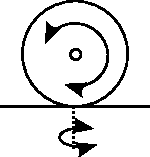
\includegraphics[width=2.5cm]{figs/wheeltype_standard.png}
\def\svgwidth{2.5cm}
\import{./figs/}{wheeltype_standard.pdf_tex}  & Front-wheel of a wheelbarrow    & Two:%
\begin{itemize}[wide=0.8\parindent,listparindent=4pt,itemsep=-2pt]
\item Rotation around the wheel axle
\item Rotation around its contact point with the ground
\end{itemize}\\
\hline
Caster wheel
% 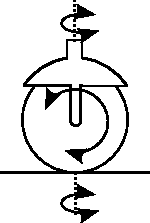
\includegraphics[width=2.5cm]{figs/wheeltype_caster.png}
\def\svgwidth{2.5cm}
\import{./figs/}{wheeltype_caster.pdf_tex}  & Office chair & Three:%
\begin{itemize}[wide=0.8\parindent,listparindent=4pt,itemsep=-2pt]
\item Rotation around the wheel axle
\item Rotation around its contact point with the ground
\item Rotation around the caster axis
\end{itemize}\\
\hline
Swedish wheel
% 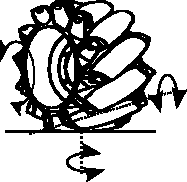
\includegraphics[width=2.5cm]{figs/wheeltype_swedish.png}
\def\svgwidth{2.5cm}
\import{./figs/}{wheeltype_swedish.pdf_tex} & Standard wheel with non-actuated rollers around its circumference& Three:%
\begin{itemize}[wide=0.8\parindent,listparindent=4pt,itemsep=-2pt]
\item Rotation around the wheel axle
\item Rotation around its contact point with the ground
\item Rotation around the roller axles
\end{itemize}\\
\hline
Spherical wheel
% 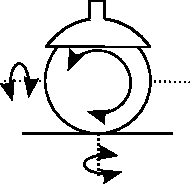
\includegraphics[width=2.5cm]{figs/wheeltype_spherical.png}
\def\svgwidth{2.5cm}
\import{./figs/}{wheeltype_spherical.pdf_tex} & Ball Bearing & Three:%
\begin{itemize}[wide=0.8\parindent,listparindent=4pt,itemsep=-2pt]
\item Rotation in any direction
\item Rotation around its contact point
\end{itemize}\\
\hline
\end{tabular}
\caption{Different types of wheels and their degrees of freedom. Adopted from \protect\citeasnoun{siegwart2011introduction}.}\label{tab:wheels}
\end{table}

Only robots that use exclusively use wheels with three degrees-of-freedom ($3$-DoF wheels) will be able to freely move on a plane. This is because the pose of a robot on a plane is fully determined by its position (two values, e.g. vertical and horizontal position) and its orientation (one value, e.g. an angle). Robots that don't have wheels with three degrees of freedom will have \textsl{kinematic constraints}\index{Kinematic constraints} that prevent them from reaching every possible point at every possible orientation. For example, a bicycle wheel can only roll along one direction and turn on the spot. Moving the bicycle wheel orthogonally to its direction of motion is not possible, unless it is forcefully dragged (``skidding''). Importantly, not having three degrees of freedom does not imply that some poses in the plane are unreachable---it may just require additional movements to achieve them!

A good analogue are figures on a chess-board. For example, a knight can reach every cell on a chess-board but might require multiple moves to do so. This is similar to a car, which can parallel park using back-and-forth motions. Instead, a bishop can only reach either black or white fields on the board, based upon its starting position.

Similar reasoning applies to aerial and underwater robots. Here, the position of the robot is affected by the position and orientation of its thrusters, either in the form of jets or propellers. Things become complicated quickly, however, as the dynamics of the system are subject to fluid-dynamic and aero-dynamic effects, which also change as a function of the size of the robot. This book will not go into the details of flying and swimming robots, but the general principles of localization and planning will be applicable to them as well.

\begin{mdframed} Think about possible wheel, propeller and thruster configurations. Don't limit yourself to robots, but consider also street and aerial vehicles and be creative---if you can think about a setup that makes sense, i.e., allows for reasonable mobility---somebody has already built it and analyzed it. What are the advantages and disadvantages of each?
\end{mdframed}

For manipulating arms, Cartesian DoFs refer to the positions and orientations (rotations around the primary axes ($x$, $y$, and $z$) that the end-effector can reach. Each actuated joint will typically add a degree of freedom, unless it is redundant (moving in the same direction, with the same physical effect, as a different joint). \cref{fig:basickinematics,fig:prismaticjointkinematics} show a series of manipulators operating on a planar surface. In such a scenario, the degrees of freedom of the end-effector are limited to moving up and down, sideways, and rotating around their pivot point. As a plane only has those three degrees of freedom, adding additional joints will not increase the number of Cartesian DoFs unless they allow the robot to also move in and out of the plane (``vertical'' axis).
%
An exact definition of the number of degrees of freedom is tricky and requires deriving analytical expressions for the end-effector position and orientation, which will be the subject of \cref{chap:kinematics}.

\begin{figure}[!htb]
    \centering
    % 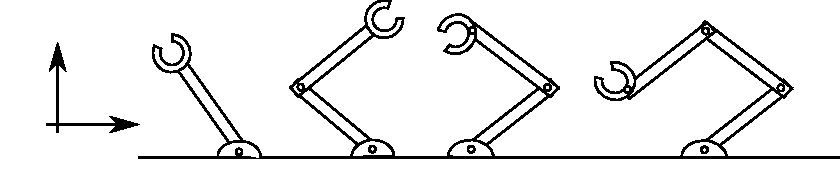
\includegraphics[width=\textwidth]{figs/basickinematics.png}
    \def\svgwidth{\textwidth}
    \import{./figs/}{basickinematics.pdf_tex}
    \caption{From left to right: Manipulators with one, two, three and four mechanical DoFs. The Cartesian DoFs needed for the end-effector to move in a plane are: the vertical displacement of the end-effector with respect to the base, its horizontal displacement, and its orientation.}
    \label{fig:basickinematics}
\end{figure}

\begin{figure}[!htb]
    \centering
    % 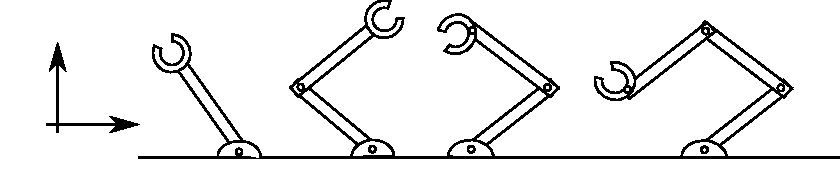
\includegraphics[width=\textwidth]{figs/basickinematics.png}
    \def\svgwidth{\textwidth}
    \import{./figs/}{prismaticjointkinematics.pdf_tex}
    \caption{From left to right: Manipulators with one, two, three, and four DoFs using a combination of rotational and prismatic joints.}
    \label{fig:prismaticjointkinematics}
\end{figure}

Choosing the ``right'' kinematics involves a very complex trade-off between mechanical complexity, maneuverability, achievable precision, cost, and ease of control. The very popular differential-wheel drive---consisting of two independently controlled wheels that share a common axis, such as those mounted on a robotic vacuum cleaner---is cheap, highly maneuverable, and easy to control; however, it is hard to drive the robot in a perfectly straight line. This motion requires both motors to turn at the exact same speed and both wheels to have the exact same diameter, which is hard to achieve in practice. This problem is solved well by car-like steering mechanisms---which in turn have poor maneuverability and are difficult to control (as a reference, think about the complexity of parallel parking).

\section{Coordinate Systems and Frames of Reference}\label{sec:coordsystems}

\screencast{http://youtu.be/klBJi-MEeNQ}{coordinatesystem}

Every robot assumes a position in the real world that can be described by its position (x, y and z) and orientation (pitch, yaw and roll) along the three major axes of a Cartesian Coordinate system (see also \cref{sec:dof}).
Such a coordinate system is shown in \cref{fig:coordinatesystem}. Note that the directions and orientations of the coordinate axes are arbitrary. This book uses the ``right hand rule'', which is illustrated in \cref{fig:coordinatesystem} to determine axes labels and directions throughout.
Pitch, yaw, and roll, are also known as bank, attitude, and heading in other communities\index{Pitch}\index{Yaw}\index{Roll}\index{Bank}\index{Attitude}\index{Heading}. This makes sense, considering the colloquial use of the word ``heading'', which corresponds to a rotation around the z-axis of a vehicle driving on the x-y-plane.

\begin{figure}
    \centering
    % 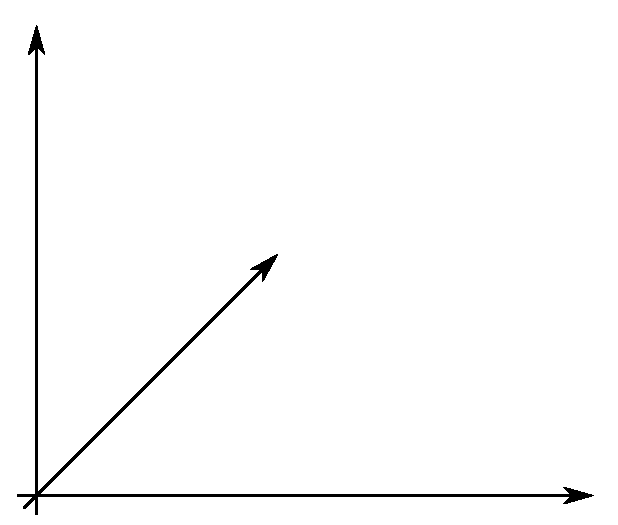
\includegraphics[width=0.8\textwidth]{figs/coordinatesystem}
    \def\svgwidth{0.8\textwidth}
    \import{./figs/}{coordinatesystem.pdf_tex}
    \caption{A coordinate system indicating the direction of the coordinate axes and rotation around them. These directions have been derived using the right-hand rules.}
    \label{fig:coordinatesystem}
\end{figure}

Defining all three position axes and orientations might be cumbersome. What level of detail we care about, where the origin of this coordinate system is, and even what kind of coordinate system we choose, depends on the specific application.
For example, a simple mobile robot would typically require a representation with respect to a room, a building, or the earth's coordinate system (given by the longitude and latitude of each point on earth), whereas a static manipulator usually has the origin of its coordinate system at its base.
More complicated systems, such as mobile manipulators or multi-legged robots, make life much easier by defining multiple coordinate systems, e.g.\ one for each leg and one that describes the position of the robot in the world frame. These local coordinate systems are known as \emph{Frames of Reference}\index{Frame of Reference}.
An example of two nested coordinate systems is shown in \cref{fig:nestedcoords}. In this example, a robot located at the origin of $x',y'$ and $z'$ might plan its motions in its own reference frame, which can then be expressed in the coordinate system $x$, $y$ and $z$ by performing a translation and a rotation---as we will later see.

Depending on its degrees of freedom in Cartesian space---that is, the number of independent translations and rotations a robot can achieve in such a space---it is also customary to ignore components of position and orientation that remain constant.
For example, a simple floor-cleaning robot's pose might be completely defined by its $x$ and $y$ coordinates in a room as well as its orientation, i.e.\ its rotation around the $z$-axis. In this case, $z$ position and rotation around $x$ and $y$ axes would be ignored.

\begin{figure}
    \centering
    %
\includegraphics[width=\textwidth]{figs/frameofreference.png}
    \def\svgwidth{\textwidth}
    \import{./figs/}{nestedcoords.pdf_tex}
    \caption{Two nested coordinate systems (also referred to as frames of reference).}
    \label{fig:nestedcoords}
\end{figure}

\subsection{Matrix notation}
Given some kind of fixed coordinate system, we can describe the \emph{position} of a robot's end-effector by a $3\times1$ position vector.
As there can be many coordinate systems defined on a robot and the environment, we identify the coordinate system a point relates to by a preceeding super-script, e.g., $ ^AP$ to indicate that point $P$ is in coordinate system $\{A\}$.
Each point consists of three elements $ ^AP=[p_x, p_y, p_z]^T$.

More formally, $^AP$ is a linear combination of the three basis vectors that span $A$:
\begin{equation}
^AP=p_x\left[\begin{array}{c}1\\0\\0\end{array}\right]+p_y\left[\begin{array}{c}0\\1\\0\end{array}\right]+p_z\left[\begin{array}{c}0\\0\\1\end{array}\right]\label{eq:basis}
\end{equation}

\screencast{http://youtu.be/QdHO_9M8-UI}{frameofreference}

As we know, not only the position of the robot is important, but also its orientation.
In order to describe the orientation of a point, we will attach a coordinate system to it. Let $ \hat{X}_B, \hat{Y}_B$ and $ \hat{Z}_B$ be unit vectors that correspond to the principal axes of a coordinate system $\{B\}$.
When expressed in coordinate system $\{A\}$, they are denoted $^A\hat{X}_B, ^A\hat{Y}_B$ and $ ^A\hat{Z}_B$.
In order to express a vector that is given in one coordinate system in another, we need to \textsl{project} each of its components to the unit vectors that span the target coordinate system. For example, if we consider only the axis $^A\hat{X}_B$, we have that:

\begin{equation}\label{eq:projection}
^A\hat{X}_B=(\hat{X}_B\cdot\hat{X}_A, \hat{X}_B\cdot\hat{Y}_A,\hat{X}_B\cdot\hat{Z}_A)^T
\end{equation}

consists of the projections of $\hat{X}_B$ onto $\hat{X}_A$, $\hat{Y}_A$ and $\hat{Z}_A$. Here, `$\cdot$' denotes the scalar product (also known as dot or inner product, see \cref{app:linalg:dotproduct}).
Note that all vectors in (\ref{eq:projection}) are unit vectors, i.e.\ their length is one.
By following the definition of the scalar product, we have that $A\cdot B=\|A\|\|B\|\cos \alpha=\cos \alpha$, indeed reduces the projection of $\hat{X}_B$ onto the unit vectors of $\{A\}$. This projection is illustrated in \cref{fig:projection}.

\begin{figure}
    \centering
    % 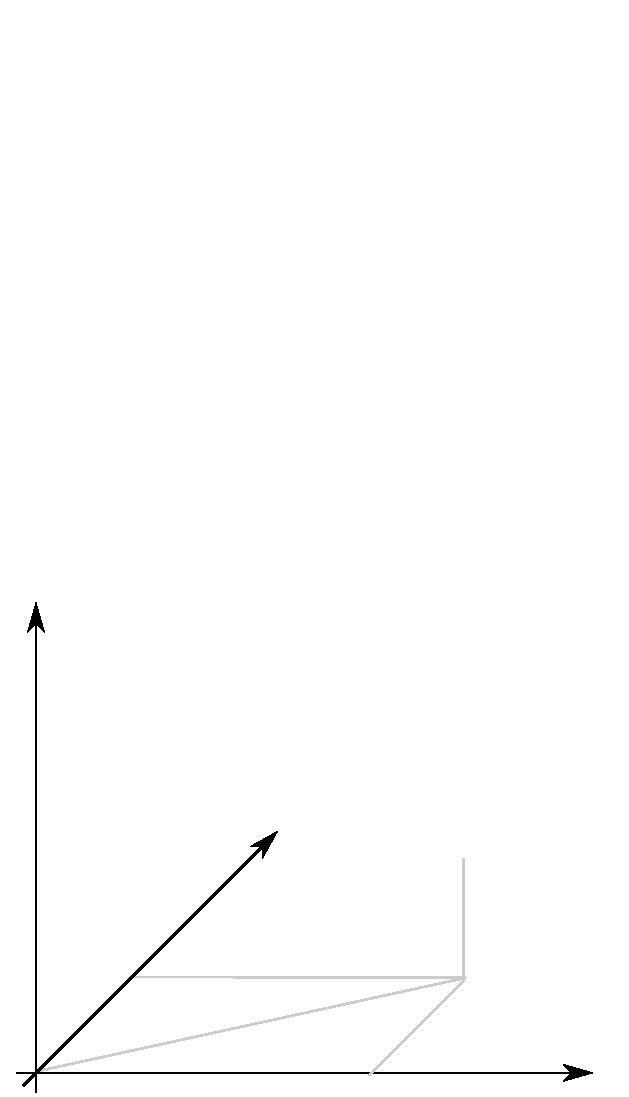
\includegraphics[width=0.8\textwidth]{figs/projection.png}
    \def\svgwidth{0.8\textwidth}
    \import{./figs/}{projection.pdf_tex}
    \caption{Top: A coordinate system $\{B\}$ with position given by $^AP$ and orientation given by $\hat{X}_B$, $\hat{Y}_B$, and $\hat{Z}_B$. Bottom:
    The projection of the unit vector $\hat{X}_B$ onto the unit vectors that span coordinate system $\{A\}$ after moving $\{B\}$ into the origin of $\{A\}$. As all vectors are unit vectors, $A\cdot B=\|A\|\|B\|\cos \alpha=\cos \alpha$. }
    \label{fig:projection}
\end{figure}

We can now apply the same procedure to all three vectors that span coordinate system $\{B\}$ and stack these three vectors together into a $3\times3$ matrix to obtain the rotation matrix
%
\begin{equation}
^A_BR=[^A\hat{X}_B \quad ^A\hat{Y}_B \quad ^A\hat{Z}_B]   ,
\end{equation}
%
which describes $\{B\}$ relative to $\{A\}$.
It is important to note that all columns in $ ^A_BR$ are unit vectors, so that the rotation matrix is orthonormal.
This is important as it allows us to easily obtain the inverse of $ ^A_BR$ as $ ^A_BR^T$ or
$ ^B_AR=^A_BR^T$.

The reason for which the unit vectors of a coordinate system $\{B\}$ expressed in coordinate system $\{A\}$ actually make up a rotation matrix can be easily seen when re-arranging Equation~\ref{eq:basis} in matrix form:
\begin{equation}
^AP=\left[\begin{array}{ccc}1 & 0 & 0\\0 & 1 & 0\\0 & 0 & 1\end{array}\right]\left[\begin{array}{c}p_x\\p_y\\p_z\end{array}\right],
\end{equation}
where the rotation matrix is nothing but the identity as both points already are in the same coordinate system. In this case, an identity matrix would signify a lack of rotation around all axes.

We have now established how to express the orientation of a coordinate system using a rotation matrix. Usually, coordinate systems don't lie on top of each other, but are also displaced from each other.
Together, position and orientation are known as a \emph{frame},\index{Frame} which is a set of four vectors, one for the position and three for the orientation, and we can write
%
\begin{equation}
\{B\}=\{^A_BR, ^AP\}
\end{equation}
%
to describe the coordinate frame $\{B\}$ with respect to $\{A\}$ using a vector $^AP$ and a rotation matrix $^A_BR$. Robots usually have many such frames defined along their bodies.

\subsection{Mapping from one frame to another}

\screencast{http://youtu.be/NsiJNvsuO3s}{rotationmatrix}

Having introduced the concept of frames, we need the ability to map coordinates in one frame to coordinates in another frame. For example, let's consider frame $\{B\}$ having the same orientation as frame $\{A\}$ and sitting at location $^AP$ in space. As the orientation of both frames is the same, we can express a point $ ^BQ$ in frame $\{A\}$ as:
%
\begin{equation}
^AQ=^BQ+^AP
\end{equation}
%
In reality, adding two vectors that are in different reference frames, i.e., $ ^BQ+^AP$, is only possible if both of them have the same orientation. We can, however, convert from one reference frame to the other using the rotation matrix:

\begin{equation}
^AP=^A_BR^BP
\end{equation}
%
and therefore solve the mapping problem regardless of the orientation of $\{A\}$ to $\{B\}$:
\begin{equation}
^AQ=^A_BR^BQ+^AP
\end{equation}
Using this notation, we can see that leading subscripts cancel the leading superscripts of the following vector/rotation matrix.
Even though we have now a solution to transform a point from one frame of reference to another by combining a rotation and a translation, it would be more appealing to write it in a more compact form, i.e.:
\begin{equation}
^AQ=^A_BT^BQ
\end{equation}
In order to do this, we need to introduce a $4\times1$ position vector such that
\begin{equation}
\left[\begin{array}{c}^AQ\\1\end{array}\right]=\left[\begin{array}{ccc|c} & ^A_BR & & ^AP \\\hline 0 & 0 & 0 & 1\end{array}\right]\left[\begin{array}{c}^BQ\\1\end{array}\right]
\end{equation}
and $^A_BT$ is a $4\times4$ matrix.  Note that the added `$1$'s and $ [0\ 0\ 0\ 1]$ do not affect the other entries in the matrix during matrix multiplication. A $4\times4$ matrix of this form is called a \emph{homogenous transform}.\index{Homogenous Transform}

The inverse of an homogeneous transform can be constructed by inverting rotation and translation part independently, leading to
\begin{equation}
\left[\begin{array}{ccc|c} & ^A_BR & & ^AP \\\hline 0 & 0 & 0 & 1\end{array}\right]^{-1}=
\left[\begin{array}{ccc|c} & ^A_BR^T & & -^A_B{R^T}{^AP} \\\hline 0 & 0 & 0 & 1\end{array}\right]
\end{equation}

We have now established a convenient notation to convert points from one coordinate system to another. There are many possible ways this can be done, in particular how rotation can be represented (see below), but all can be converted from one into the other.

\subsection{Transformation arithmetic}

Transformations can be combined: consider for example an arm with two links, reference frame $\{A\}$ at the base, $ \{B\} $ at its first joint, and $\{C\}$ at its end-effector. Given the transforms $ ^B_CT$ and $ ^A_BT$, we can write
\begin{equation}
^AP=^A_BT^B_CT^CP=^A_CT^CP
\end{equation}
to convert a point in the reference frame of the end-effector to that of its base. As this works for rotation and translation operators independently, we can construct $ ^A_CT$ as
\begin{equation}
^A_CT=\left[\begin{array}{ccc|c} & ^A_BR^B_CR & & ^A_BR^BP_C +^AP_B \\\hline 0 & 0 & 0 & 1\end{array}\right]
\end{equation}
%
where $ ^AP_B$ and $ ^BP_C$ are the translations from $\{A\}$ to $\{B\}$ and from $ \{B\}$ to $\{C\}$, respectively.

\subsection{Other representations for orientation}

So far, we have represented orientation by a $3\times3$ matrix whose column vectors are orthogononal unit vectors describing the orientation of a coordinate system. Orientation is therefore represented with nine different values. We chose this representation mainly because it is the most intuitive to explain and is derived from simple geometry.

In fact, three values are sufficient to describe orientation.
This becomes clear when considering that orthogonality (dot product of all columns is zero) and vector length (each vector must have length $1$) impose six constraints on the nine values in the rotation matrix.
Indeed, an orientation can be represented as a rotation by certain angles around the $x-$, the $y-$, and the $z$-axis of the reference coordinate system. This is known as the X-Y-Z fixed-angle notation.\index{Fixed angle notation} Mathematically, this can be represented by a rotation matrix of the form:
\begin{equation}
^A_BR_{XYZ}(\gamma,\beta,\alpha)=\begin{bsmallmatrix}cos\alpha & -sin\alpha & 0\\sin\alpha & \cos\alpha & 0\\0 & 0 & 1\end{bsmallmatrix}\begin{bsmallmatrix}cos\beta& 0 & sin\beta\\0 & 1 & 0\\-sin\beta & 0 & cos\beta\end{bsmallmatrix}\begin{bsmallmatrix}1 & 0 & 0 \\ 0 & cos\gamma & -sin\gamma\\0 & sin\gamma & cos\gamma\end{bsmallmatrix}
\end{equation}

While the $X-Y-Z$ fixed angles approach expresses a coordinate frame using rotations with respect to the original coordinate frame (say, $\{A\}$), another possible description is to start with a coordinate frame $\{B\}$ that is coincident with frame $\{A\}$, then rotate around the Z-axis with angle $ \alpha$, then the Y-axis with angle $ \beta$ and finally around the X-axis with angle $ \gamma$. This representation is called Z-Y-X Euler angles.\index{Euler angles}
As the coordinate axis do not necessarily need to be different, there are twelve possible valid combinations of sub-sequent rotations: XYX, XZX, YXY, YZY, ZXZ, ZYZ, XYZ, XZY, YZX, YXZ, ZXY and ZYX.
The reason for which there are only twelve is that sub-sequent rotations around the same axis are not valid. Such rotations would not add any information, but are equivalent to a rotation by the sum of both angles.

It is important to know about the subtle differences between the available transformations as there is neither ``right'' nor ``wrong'' convention, however different manufacturers and fields use different ones.
There is only one caveat: each of the rotation matrices can look like subsequent rotations around the same axis for certain values of angles. For example, this happens for the XYZ rotation matrix if the angle of rotation around the Y-axis is $90^\circ$. These cases are known as a \emph{singularities} of the specific notation.\index{Singularity}

Among the many conventions, the preferred representation for computational and stability reasons are \emph{quaternions}\index{Quaternion}.
A quaternion is a 4-tuple that extends the complex numbers with very general applications in mathematics and representing orientation and rotation in particular. The basic idea is that each rotation can be represented as a rotation around a single axis (a vector in space) by a specific angle. Given such an axis $ \hat{K}=[k_x k_y k_z]^T$ and an angle $ \theta$, one can calculate the so-called Euler parameters\index{Euler parameters} or unit quaternion\index{unit quaternion}:

\begin{eqnarray}
\epsilon_1=k_x sin \frac{\theta}{2}\\
\epsilon_2=k_y sin \frac{\theta}{2}\\
\epsilon_3=k_z sin \frac{\theta}{2}\\
\epsilon_4=cos\frac{\theta}{2}
\end{eqnarray}

These four quantities are constrained by the relationship
\begin{equation}
\epsilon_1^2+\epsilon_2^2+\epsilon_3^2+\epsilon_4^2=1,
\end{equation}
which might be visualized by a point on a unit hyper-sphere. %Transformations are represented by \emph{dual quaternions}\index{Dual quaternion}, one for the translation and one for the rotation. Dual quaternions can again easily be converted into homogenous transformation matrices.
Analogous to rotation matrices, two quaternions $\epsilon$ and $\epsilon'$ can be multiplied using the following equation
\begin{equation}
\left[
\begin{array}{cccc}
\epsilon_4 & \epsilon_1 & \epsilon_2 & \epsilon_3\\
-\epsilon_1 & \epsilon_4 & -\epsilon_3 & \epsilon_2\\
-\epsilon_2 & \epsilon_3 & \epsilon_4 & -\epsilon_1\\
-\epsilon_3 & -\epsilon_2 & \epsilon_1 & \epsilon_4
\end{array}
\right]
\left[\begin{array}{c}\epsilon_4'\\\epsilon_1'\\\epsilon_2'\\\epsilon_3'\end{array}\right]
\end{equation}

Unlike multiplying two rotation matrices, which requires 27 multiplications and 18 additions, multiplying two quaternions only requires 16 multiplications and 12 additions, making the operation computationally more efficient.
Importantly, this representation does not suffer from singularities for specific joint angles, making the approach computationally more robust. This is particularly relevant for robotics, as mathematical singularities have pretty significant real-world impact on physical robots (see e.g. \cref{sec:invjac}).

Why any rotation can be expressed by a single vector can be seen when considering the properties of orthonomal rotation matrices. They have three eigenvalues $\lambda=1$ and a complex pair $\lambda_{1,2}=\cos \theta \pm i \sin \theta$.
Eigenvalues and eigenvectors are defined as $Rv=\lambda v$. For the case of $\lambda=1$, the corresponding Eigenvector $v$ is unchanged by rotation. This is only possible if $v$ is the actual axis of rotation.
The angle of rotation is now given by $\theta$, which can be inferred from the complex pair.



\section*{Take-home lessons}

\begin{itemize}
\item In order to perform planning for a robot, it is necessary to understand how its control parameters map to actions in the physical world.
\item The kinematics of a robot are fully defined by the position and orientation of its wheels, joints and links no matter whether it swims, flies, crawls or drives.
\item Many robotic systems cannot be fully understood by considering kinematics alone, but require you to model their dynamics as well. This book will be limited to modeling kinematics, which is sufficient for low-speed mobile robots and arms.
\end{itemize}


\section*{Exercises}\small
\begin{enumerate}
\item What are the Cartesian DoFs of a push lawnmower with four wheels? How is it still possible to mow an entire lawn with one, even though the wheels don't yaw?
\item Is a car statically or dynamically stable? What about a motorcycle?
\item What are the Cartesian DoFs of an office chair with all caster-wheels?
\item What are the maximum Cartesian DoFs for orientable objects driving on the 2D plane?
\item What are the maximum Cartesian DoFs for objects that can freely translate and rotate in the world?
\item Calculate the Cartesian DoFs of a differential drive robot with two powered rear wheels and a central, front-mounted caster wheel. What happens when you add a second caster wheel?
\item Calculate the Cartesian DoFs of a standard car. How is it possible to still reach every point on the plane?
\item A steering wheel allows you to change the yaw of your car. Can you also change its pitch and its roll? See \cref{fig:pitchyawandroll} for reference.
\end{enumerate}\normalsize

\chapter{Kinematics}\label{chap:kinematics}

In order to plan a robot's movements, we have to understand the relationship between the actuators that we can control and the robot's resulting position in the environment. For static arms, this is rather straightforward: if we know the position/angle of each joint, we can calculate the position of its end-effectors using trigonometry. This process is known as \emph{forward kinematics}. \index{Forward Kinematics} If we want to calculate the position each joint needs to be at, we need to invert this relationship. This is known as \emph{inverse kinematics}. \index{Inverse Kinematics} For mobile robots, this process is usually more involved, as speeds need to be integrated, which we refer to as \emph{odometry}\index{Odometry}.

The goals of this chapter are:

\begin{itemize}
\item to introduce coordinate systems and their transformations;
\item to introduce the forward kinematics of simple arms and mobile robots;
\item to understand the concept of holonomy;
\item to show how solutions for the inverse kinematics for both static and mobile robots can be derived;
\item to provide an intuition on the relationship between inverse kinematics and path-planning.
\end{itemize}

%%%%%%%%%%%%%%%%%%%%
%% ACTUAL CONTENT %%
%%%%%%%%%%%%%%%%%%%%

\section{Coordinate Systems and Frames of Reference}\label{sec:coordsystems}

\screencast{http://youtu.be/klBJi-MEeNQ}{coordinatesystem}

Every robot assumes a position in the real world that can be described by its position (x, y and z) and orientation (pitch, yaw and roll) along the three major axes of a Cartesian Coordinate system (see also \cref{sec:dof}).
Such a coordinate system is shown in \cref{fig:coordinatesystem}. Note that the directions and orientations of the coordinate axes are arbitrary. This book uses the ``right hand rule'', which is illustrated in \cref{fig:coordinatesystem} to determine axes labels and directions throughout.
Pitch, yaw, and roll, are also known as bank, attitude, and heading in other communities\index{Pitch}\index{Yaw}\index{Roll}\index{Bank}\index{Attitude}\index{Heading}. This makes sense, considering the colloquial use of the word ``heading'', which corresponds to a rotation around the z-axis of a vehicle driving on the x-y-plane.

\begin{figure}
    \centering
    % 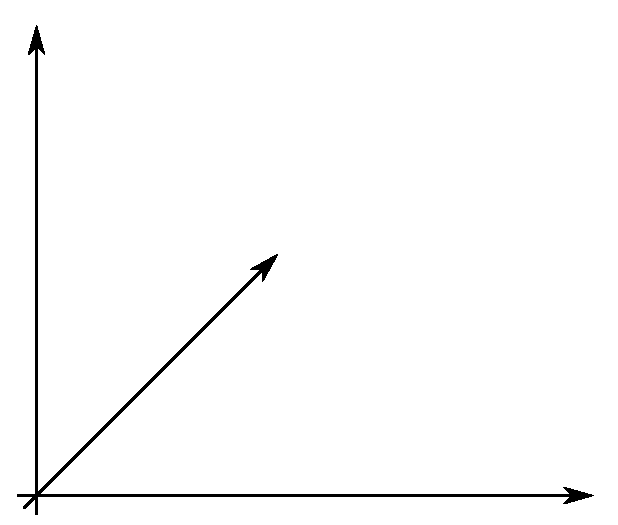
\includegraphics[width=0.8\textwidth]{figs/coordinatesystem}
    \def\svgwidth{0.8\textwidth}
    \import{./figs/}{coordinatesystem.pdf_tex}
    \caption{A coordinate system indicating the direction of the coordinate axes and rotation around them. These directions have been derived using the right-hand rules.}
    \label{fig:coordinatesystem}
\end{figure}

Defining all three position axes and orientations might be cumbersome. What level of detail we care about, where the origin of this coordinate system is, and even what kind of coordinate system we choose, depends on the specific application.
For example, a simple mobile robot would typically require a representation with respect to a room, a building, or the earth's coordinate system (given by the longitude and latitude of each point on earth), whereas a static manipulator usually has the origin of its coordinate system at its base.
More complicated systems, such as mobile manipulators or multi-legged robots, make life much easier by defining multiple coordinate systems, e.g.\ one for each leg and one that describes the position of the robot in the world frame. These local coordinate systems are known as \emph{Frames of Reference}\index{Frame of Reference}.
An example of two nested coordinate systems is shown in \cref{fig:nestedcoords}. In this example, a robot located at the origin of $x',y'$ and $z'$ might plan its motions in its own reference frame, which can then be expressed in the coordinate system $x$, $y$ and $z$ by performing a translation and a rotation---as we will later see.

Depending on its degrees of freedom in Cartesian space---that is, the number of independent translations and rotations a robot can achieve in such a space---it is also customary to ignore components of position and orientation that remain constant.
For example, a simple floor-cleaning robot's pose might be completely defined by its $x$ and $y$ coordinates in a room as well as its orientation, i.e.\ its rotation around the $z$-axis. In this case, $z$ position and rotation around $x$ and $y$ axes would be ignored.

\begin{figure}
    \centering
    %
\includegraphics[width=\textwidth]{figs/frameofreference.png}
    \def\svgwidth{\textwidth}
    \import{./figs/}{nestedcoords.pdf_tex}
    \caption{Two nested coordinate systems (also referred to as frames of reference).}
    \label{fig:nestedcoords}
\end{figure}

\subsection{Matrix notation}
Given some kind of fixed coordinate system, we can describe the \emph{position} of a robot's end-effector by a $3\times1$ position vector.
As there can be many coordinate systems defined on a robot and the environment, we identify the coordinate system a point relates to by a preceeding super-script, e.g., $ ^AP$ to indicate that point $P$ is in coordinate system $\{A\}$.
Each point consists of three elements $ ^AP=[p_x, p_y, p_z]^T$.

More formally, $^AP$ is a linear combination of the three basis vectors that span $A$:
\begin{equation}
^AP=p_x\left[\begin{array}{c}1\\0\\0\end{array}\right]+p_y\left[\begin{array}{c}0\\1\\0\end{array}\right]+p_z\left[\begin{array}{c}0\\0\\1\end{array}\right]\label{eq:basis}
\end{equation}

\screencast{http://youtu.be/QdHO_9M8-UI}{frameofreference}

As we know, not only the position of the robot is important, but also its orientation.
In order to describe the orientation of a point, we will attach a coordinate system to it. Let $ \hat{X}_B, \hat{Y}_B$ and $ \hat{Z}_B$ be unit vectors that correspond to the principal axes of a coordinate system $\{B\}$.
When expressed in coordinate system $\{A\}$, they are denoted $^A\hat{X}_B, ^A\hat{Y}_B$ and $ ^A\hat{Z}_B$.
In order to express a vector that is given in one coordinate system in another, we need to \textsl{project} each of its components to the unit vectors that span the target coordinate system. For example, if we consider only the axis $^A\hat{X}_B$, we have that:

\begin{equation}\label{eq:projection}
^A\hat{X}_B=(\hat{X}_B\cdot\hat{X}_A, \hat{X}_B\cdot\hat{Y}_A,\hat{X}_B\cdot\hat{Z}_A)^T
\end{equation}

consists of the projections of $\hat{X}_B$ onto $\hat{X}_A$, $\hat{Y}_A$ and $\hat{Z}_A$. Here, `$\cdot$' denotes the scalar product (also known as dot or inner product, see \cref{app:linalg:dotproduct}).
Note that all vectors in (\ref{eq:projection}) are unit vectors, i.e.\ their length is one.
By following the definition of the scalar product, we have that $A\cdot B=\|A\|\|B\|\cos \alpha=\cos \alpha$, indeed reduces the projection of $\hat{X}_B$ onto the unit vectors of $\{A\}$. This projection is illustrated in \cref{fig:projection}.

\begin{figure}
    \centering
    % 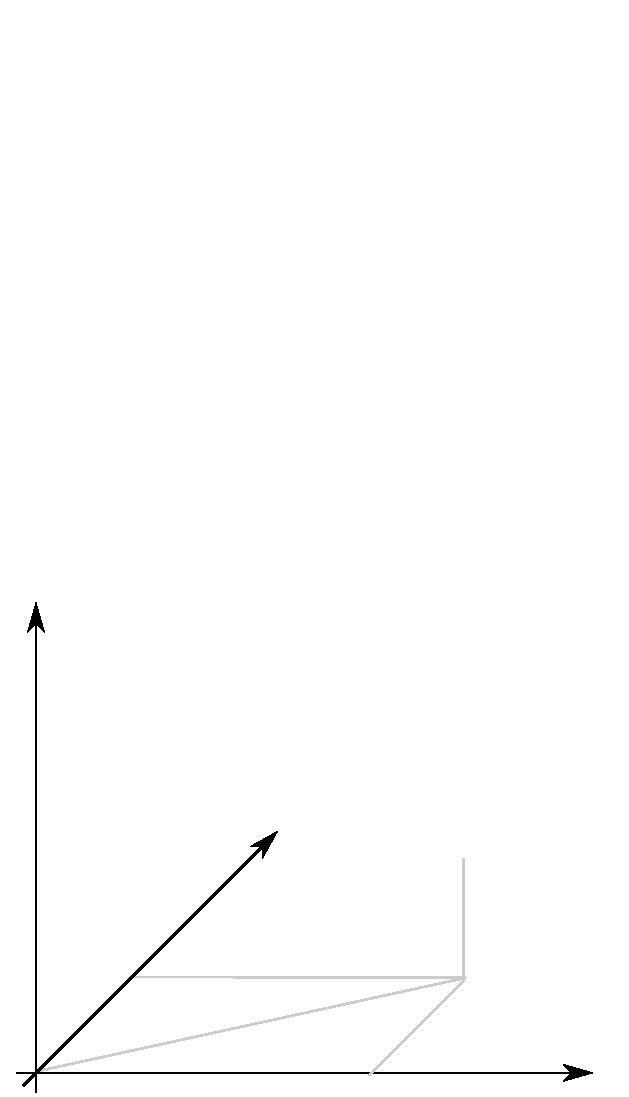
\includegraphics[width=0.8\textwidth]{figs/projection.png}
    \def\svgwidth{0.8\textwidth}
    \import{./figs/}{projection.pdf_tex}
    \caption{Top: A coordinate system $\{B\}$ with position given by $^AP$ and orientation given by $\hat{X}_B$, $\hat{Y}_B$, and $\hat{Z}_B$. Bottom:
    The projection of the unit vector $\hat{X}_B$ onto the unit vectors that span coordinate system $\{A\}$ after moving $\{B\}$ into the origin of $\{A\}$. As all vectors are unit vectors, $A\cdot B=\|A\|\|B\|\cos \alpha=\cos \alpha$. }
    \label{fig:projection}
\end{figure}

We can now apply the same procedure to all three vectors that span coordinate system $\{B\}$ and stack these three vectors together into a $3\times3$ matrix to obtain the rotation matrix
%
\begin{equation}
^A_BR=[^A\hat{X}_B \quad ^A\hat{Y}_B \quad ^A\hat{Z}_B]   ,
\end{equation}
%
which describes $\{B\}$ relative to $\{A\}$.
It is important to note that all columns in $ ^A_BR$ are unit vectors, so that the rotation matrix is orthonormal.
This is important as it allows us to easily obtain the inverse of $ ^A_BR$ as $ ^A_BR^T$ or
$ ^B_AR=^A_BR^T$.

The reason for which the unit vectors of a coordinate system $\{B\}$ expressed in coordinate system $\{A\}$ actually make up a rotation matrix can be easily seen when re-arranging Equation~\ref{eq:basis} in matrix form:
\begin{equation}
^AP=\left[\begin{array}{ccc}1 & 0 & 0\\0 & 1 & 0\\0 & 0 & 1\end{array}\right]\left[\begin{array}{c}p_x\\p_y\\p_z\end{array}\right],
\end{equation}
where the rotation matrix is nothing but the identity as both points already are in the same coordinate system. In this case, an identity matrix would signify a lack of rotation around all axes.

We have now established how to express the orientation of a coordinate system using a rotation matrix. Usually, coordinate systems don't lie on top of each other, but are also displaced from each other.
Together, position and orientation are known as a \emph{frame},\index{Frame} which is a set of four vectors, one for the position and three for the orientation, and we can write
%
\begin{equation}
\{B\}=\{^A_BR, ^AP\}
\end{equation}
%
to describe the coordinate frame $\{B\}$ with respect to $\{A\}$ using a vector $^AP$ and a rotation matrix $^A_BR$. Robots usually have many such frames defined along their bodies.

\subsection{Mapping from one frame to another}

\screencast{http://youtu.be/NsiJNvsuO3s}{rotationmatrix}

Having introduced the concept of frames, we need the ability to map coordinates in one frame to coordinates in another frame. For example, let's consider frame $\{B\}$ having the same orientation as frame $\{A\}$ and sitting at location $^AP$ in space. As the orientation of both frames is the same, we can express a point $ ^BQ$ in frame $\{A\}$ as:
%
\begin{equation}
^AQ=^BQ+^AP
\end{equation}
%
In reality, adding two vectors that are in different reference frames, i.e., $ ^BQ+^AP$, is only possible if both of them have the same orientation. We can, however, convert from one reference frame to the other using the rotation matrix:

\begin{equation}
^AP=^A_BR^BP
\end{equation}
%
and therefore solve the mapping problem regardless of the orientation of $\{A\}$ to $\{B\}$:
\begin{equation}
^AQ=^A_BR^BQ+^AP
\end{equation}
Using this notation, we can see that leading subscripts cancel the leading superscripts of the following vector/rotation matrix.
Even though we have now a solution to transform a point from one frame of reference to another by combining a rotation and a translation, it would be more appealing to write it in a more compact form, i.e.:
\begin{equation}
^AQ=^A_BT^BQ
\end{equation}
In order to do this, we need to introduce a $4\times1$ position vector such that
\begin{equation}
\left[\begin{array}{c}^AQ\\1\end{array}\right]=\left[\begin{array}{ccc|c} & ^A_BR & & ^AP \\\hline 0 & 0 & 0 & 1\end{array}\right]\left[\begin{array}{c}^BQ\\1\end{array}\right]
\end{equation}
and $^A_BT$ is a $4\times4$ matrix.  Note that the added `$1$'s and $ [0\ 0\ 0\ 1]$ do not affect the other entries in the matrix during matrix multiplication. A $4\times4$ matrix of this form is called a \emph{homogenous transform}.\index{Homogenous Transform}

The inverse of an homogeneous transform can be constructed by inverting rotation and translation part independently, leading to
\begin{equation}
\left[\begin{array}{ccc|c} & ^A_BR & & ^AP \\\hline 0 & 0 & 0 & 1\end{array}\right]^{-1}=
\left[\begin{array}{ccc|c} & ^A_BR^T & & -^A_B{R^T}{^AP} \\\hline 0 & 0 & 0 & 1\end{array}\right]
\end{equation}

We have now established a convenient notation to convert points from one coordinate system to another. There are many possible ways this can be done, in particular how rotation can be represented (see below), but all can be converted from one into the other.

\subsection{Transformation arithmetic}

Transformations can be combined: consider for example an arm with two links, reference frame $\{A\}$ at the base, $ \{B\} $ at its first joint, and $\{C\}$ at its end-effector. Given the transforms $ ^B_CT$ and $ ^A_BT$, we can write
\begin{equation}
^AP=^A_BT^B_CT^CP=^A_CT^CP
\end{equation}
to convert a point in the reference frame of the end-effector to that of its base. As this works for rotation and translation operators independently, we can construct $ ^A_CT$ as
\begin{equation}
^A_CT=\left[\begin{array}{ccc|c} & ^A_BR^B_CR & & ^A_BR^BP_C +^AP_B \\\hline 0 & 0 & 0 & 1\end{array}\right]
\end{equation}
%
where $ ^AP_B$ and $ ^BP_C$ are the translations from $\{A\}$ to $\{B\}$ and from $ \{B\}$ to $\{C\}$, respectively.

\subsection{Other representations for orientation}

So far, we have represented orientation by a $3\times3$ matrix whose column vectors are orthogononal unit vectors describing the orientation of a coordinate system. Orientation is therefore represented with nine different values. We chose this representation mainly because it is the most intuitive to explain and is derived from simple geometry.

In fact, three values are sufficient to describe orientation.
This becomes clear when considering that orthogonality (dot product of all columns is zero) and vector length (each vector must have length $1$) impose six constraints on the nine values in the rotation matrix.
Indeed, an orientation can be represented as a rotation by certain angles around the $x-$, the $y-$, and the $z$-axis of the reference coordinate system. This is known as the X-Y-Z fixed-angle notation.\index{Fixed angle notation} Mathematically, this can be represented by a rotation matrix of the form:
\begin{equation}
^A_BR_{XYZ}(\gamma,\beta,\alpha)=\begin{bsmallmatrix}cos\alpha & -sin\alpha & 0\\sin\alpha & \cos\alpha & 0\\0 & 0 & 1\end{bsmallmatrix}\begin{bsmallmatrix}cos\beta& 0 & sin\beta\\0 & 1 & 0\\-sin\beta & 0 & cos\beta\end{bsmallmatrix}\begin{bsmallmatrix}1 & 0 & 0 \\ 0 & cos\gamma & -sin\gamma\\0 & sin\gamma & cos\gamma\end{bsmallmatrix}
\end{equation}

While the $X-Y-Z$ fixed angles approach expresses a coordinate frame using rotations with respect to the original coordinate frame (say, $\{A\}$), another possible description is to start with a coordinate frame $\{B\}$ that is coincident with frame $\{A\}$, then rotate around the Z-axis with angle $ \alpha$, then the Y-axis with angle $ \beta$ and finally around the X-axis with angle $ \gamma$. This representation is called Z-Y-X Euler angles.\index{Euler angles}
As the coordinate axis do not necessarily need to be different, there are twelve possible valid combinations of sub-sequent rotations: XYX, XZX, YXY, YZY, ZXZ, ZYZ, XYZ, XZY, YZX, YXZ, ZXY and ZYX.
The reason for which there are only twelve is that sub-sequent rotations around the same axis are not valid. Such rotations would not add any information, but are equivalent to a rotation by the sum of both angles.

It is important to know about the subtle differences between the available transformations as there is neither ``right'' nor ``wrong'' convention, however different manufacturers and fields use different ones.
There is only one caveat: each of the rotation matrices can look like subsequent rotations around the same axis for certain values of angles. For example, this happens for the XYZ rotation matrix if the angle of rotation around the Y-axis is $90^\circ$. These cases are known as a \emph{singularities} of the specific notation.\index{Singularity}

Among the many conventions, the preferred representation for computational and stability reasons are \emph{quaternions}\index{Quaternion}.
A quaternion is a 4-tuple that extends the complex numbers with very general applications in mathematics and representing orientation and rotation in particular. The basic idea is that each rotation can be represented as a rotation around a single axis (a vector in space) by a specific angle. Given such an axis $ \hat{K}=[k_x k_y k_z]^T$ and an angle $ \theta$, one can calculate the so-called Euler parameters\index{Euler parameters} or unit quaternion\index{unit quaternion}:

\begin{eqnarray}
\epsilon_1=k_x sin \frac{\theta}{2}\\
\epsilon_2=k_y sin \frac{\theta}{2}\\
\epsilon_3=k_z sin \frac{\theta}{2}\\
\epsilon_4=cos\frac{\theta}{2}
\end{eqnarray}

These four quantities are constrained by the relationship
\begin{equation}
\epsilon_1^2+\epsilon_2^2+\epsilon_3^2+\epsilon_4^2=1,
\end{equation}
which might be visualized by a point on a unit hyper-sphere. %Transformations are represented by \emph{dual quaternions}\index{Dual quaternion}, one for the translation and one for the rotation. Dual quaternions can again easily be converted into homogenous transformation matrices.
Analogous to rotation matrices, two quaternions $\epsilon$ and $\epsilon'$ can be multiplied using the following equation
\begin{equation}
\left[
\begin{array}{cccc}
\epsilon_4 & \epsilon_1 & \epsilon_2 & \epsilon_3\\
-\epsilon_1 & \epsilon_4 & -\epsilon_3 & \epsilon_2\\
-\epsilon_2 & \epsilon_3 & \epsilon_4 & -\epsilon_1\\
-\epsilon_3 & -\epsilon_2 & \epsilon_1 & \epsilon_4
\end{array}
\right]
\left[\begin{array}{c}\epsilon_4'\\\epsilon_1'\\\epsilon_2'\\\epsilon_3'\end{array}\right]
\end{equation}

Unlike multiplying two rotation matrices, which requires 27 multiplications and 18 additions, multiplying two quaternions only requires 16 multiplications and 12 additions, making the operation computationally more efficient.
Importantly, this representation does not suffer from singularities for specific joint angles, making the approach computationally more robust. This is particularly relevant for robotics, as mathematical singularities have pretty significant real-world impact on physical robots (see e.g. \cref{sec:invjac}).

Why any rotation can be expressed by a single vector can be seen when considering the properties of orthonomal rotation matrices. They have three eigenvalues $\lambda=1$ and a complex pair $\lambda_{1,2}=\cos \theta \pm i \sin \theta$.
Eigenvalues and eigenvectors are defined as $Rv=\lambda v$. For the case of $\lambda=1$, the corresponding Eigenvector $v$ is unchanged by rotation. This is only possible if $v$ is the actual axis of rotation.
The angle of rotation is now given by $\theta$, which can be inferred from the complex pair.

%!TEX root = ../book.tex
\section{Forward Kinematics}\label{sec:kinematics:fwkarm}

Now that we have introduced the notion of local coordinate frames, we are interested in calculating the pose and speed of these coordinate frames as a function of the robot's actuators and joint configuration.
We will first consider simple mechanisms where we can determine the relationship between actuators and the pose of various frames on the robot both in the position and speed domain. We will then consider the special class of non-holonomous mechanisms using a series of wheeled robots, for which the forward kinematics can only be calculated in the speed domain.

\subsection{Forward Kinematics of a simple robot arm}

\begin{figure}[!htb]%{L}{0.3\textwidth}
    \centering
    % 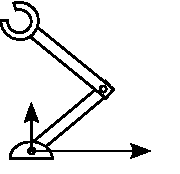
\includegraphics[width=0.27\textwidth]{figs/fwk2dofarm}
    \def\svgwidth{0.4\textwidth}
    \import{./figs/}{fwk2dofarm.pdf_tex}
    \caption{A simple 2-DOF arm.}\label{fig:fwk2dofarm}
\end{figure}

Consider the robot arm in \cref{fig:fwk2dofarm}; it is mounted to a table, and is composed of two links and two joints. Let the length of the first link be $l_1$ and the length of the second link be $l_2$. You could specify the position of the link closer to the table by the angle $\alpha$ and the angle of the second link relative to the first link using the angle $\beta$.

We can now calculate the position $P_1 = (x_1, y_1)$ of the joint between the first and the second link using simple trigonometry:
%
\begin{eqnarray}\label{eq:cosxl1}
x_1 &=&l_1 \cos \alpha \nonumber \\
y_1 &=&l_1 \sin \alpha
\end{eqnarray}
%
Similarly, the position of the end-effector $P_2 = (x_2, y_2)$ is given by:
%
\begin{eqnarray}
x_2&=&x_1 + l_2 \cos(\alpha+\beta) \nonumber \\
y_2&=&y_1 + l_2 \sin(\alpha+\beta)
\end{eqnarray}
%
or together, the position of the end-effector $(x,y)$ is given by
%
\begin{eqnarray}\label{eq:cosx}
x&=&l_1 \cos \alpha + l_2 \cos(\alpha+\beta) \nonumber \\
y&=&l_1 \sin \alpha + l_2 \sin(\alpha+\beta)
\end{eqnarray}
%
The above equations represent \textsl{the forward kinematic equations} of the robot---as they relate its control parameters $ \alpha$ and $\beta$ (also known as joint configuration) to the position of its end-effector in the local coordinate system spanned by $ x$ and $ y$ with the origin at the robot's base.
Note that both $\alpha$ and $\beta$ shown in the figure are positive: both links rotate around the $z-$axis. Using the right-hand rule, the direction of positive angles is defined to be counter-clockwise.

The \emph{configuration space}\index{Configuration space}\index{C-Space (Configuration space)} of the robot---i.e. the set of angles each actuator can be set to---is given by $ 0 < \alpha < \pi $ as it is not supposed to run into the table, and $ -\pi < \beta < \pi$.
The configuration space is given with respect to the robot's joints and allows us to use the forward kinematics equations to calculate the \emph{workspace}\index{Workspace} of the robot, i.e. the physical space it can move to.
This terminology will be identical for mobile robots. An example of configuration and workspace for both a manipulator and a mobile robot is shown in \cref{fig:holonomy}.

As shown in \cref{fig:fwk2dofarm}, the orientation of the arm's end-effector is given by $\alpha+\beta$. We can now write down  a transformation that includes a rotation around the z-axis:
\begin{equation}
\label{eq:2armtrans}
\left[\begin{array}{cccc}cos_{\alpha\beta} & -sin_{\alpha\beta} &  0 & \cos_{\alpha\beta}l_2+\cos\alpha l_1\\
                        sin_{\alpha\beta} & cos_{\alpha\beta} & 0 & \sin_{\alpha\beta}l_2+\sin\alpha l_1\\
                                                0 & 0 & 1 & 0\\
                                                0 & 0 & 0 & 1\end{array}\right]
\end{equation}
The notation $sin_{\alpha\beta}$ and $cos_{\alpha\beta}$ are shorthand for $sin(\alpha+\beta)$ and $cos(\alpha+\beta)$, respectively.

This transformation now allows us to translate from the robot's base to the robot's end-effector as a function of the joint configuration $\alpha$ and $\beta$.
This transformation will be helpful if we want to calculate suitable joint angles in order to reach a certain pose or if we want to convert measurements taken relative to the end-effector back into the base's coordinate system.

\subsection{Forward Kinematics of a Differential Wheels Robot}\label{sec:kinematics:fwkmobile}

Whereas the pose of a robotic manipulator is uniquely defined by its joint angles---which can be made available using encoders in almost real-time, see \cref{sec:sensors:encoders}---this is not the case for a mobile robot.
Here, the encoder values simply refer to wheel orientation and need to be integrated over time in order to assess the robot's position with respect to the worlds frame of reference; as we will later see, this is a great source of uncertainty.
What complicates matters is that for so-called \emph{non-holonomic} systems, it is not sufficient to simply measure the distance that each wheel traveled, but also when each movement was executed.

\begin{figure}
    \small
    \centering
    % 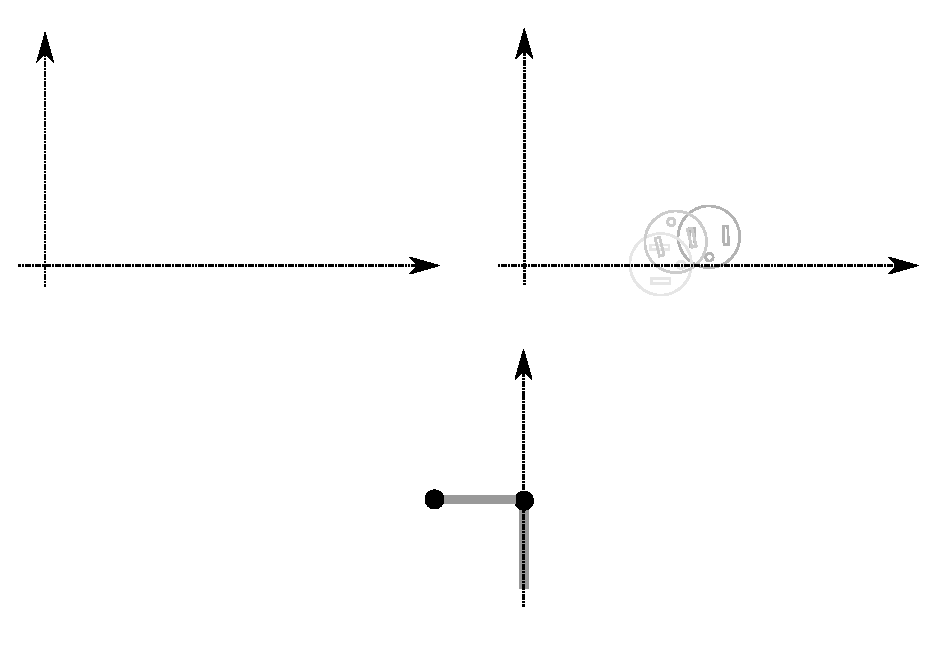
\includegraphics[width=0.95\textwidth]{figs/holonomy.png}
    \def\svgwidth{\textwidth}
    \import{./figs/}{holonomy.pdf_tex}
    \caption{Configuration or joint space (left) and workspace or operational space (right) for a non-holonomic mobile robot (top) and a holonomic manipulator (bottom). Closed trajectories in configuration space result in closed trajectories in the workspace if the robot's kinematics is holonomic.}
    \label{fig:holonomy}
\end{figure}

A system is non-holonomic\index{Non-holonomic}\index{Holonomic} when closed trajectories in its configuration space may not have it return to its original state (reminder: the configuration or joint space space of a two-link robotic arm is spanned by the possible values of each angle).
A simple arm is holonomic because each joint position corresponds to a unique position in space:
going through whatever trajectory that comes back to the starting point in configuration space, will put the robot's end-effector at the exact same position in operational space.
A train on a track is holonomic: moving its wheels backwards by the same amount they have been moving forward brings the train to the exact same position in space.
A car and a differential-wheel robot are non-holonomic vehicles: performing a straight line and then a right-turn leads to the same amount of wheel rotation than doing a right turn first and then going in a straight line; however getting the robot to its initial position requires not only to rewind both wheels by the same amount, but also getting their relative speeds right.
The configuration and corresponding workspace trajectories for a non-holonomic and a holonomic robot are shown in \cref{fig:holonomy}.
Here, a robot first moves on a straight line, i.e. both wheels turn an equal amount.
Then, the left wheel remains fixed and only the right wheel turns forward.
Then, the right wheel remain fixed and the left wheel turns backward.
Finally, the right wheel turns backward, arriving at the initial encoder values (zero).
Yet, the robot does not return to its origin. Performing a similar trajectory in the configuration space of a two-link manipulator instead, lets the robot return to its initial position.

It should be clear by now that for a mobile robot, not only traveled distance per wheel matters, but also the \textsl{speed} of each wheel as a function of time.
Interestingly however, this information was not required to uniquely determine the pose of a manipulating arm.
Let's introduce the following conventions.
We will establish a world coordinate system $\{I\}$---which is known as the inertial frame by convention (see \cref{fig:mobilerobot}).
We establish a coordinate system $\{R\}$ on the robot and express the robot's speed $^R\dot{\xi}$ as a vector $ ^R\dot{\xi}=[^R\dot{x}, ^R\dot{y}, ^R\dot{\theta}]^T$. Here $^R\dot{x}$ and $^R\dot{y}$ correspond to the speed along the $x$ and $y$ directions in $\{R\}$, whereas $^R\dot{\theta}$ corresponds to the rotation velocity around the $z-$axis, that you can imagine to be sticking out of the ground.
We denote speeds with dots over the variable name, as speed is simply the derivative of distance.
Now, let's think about the robot's position in $\{R\}$. It is always zero, as the coordinate system is fixed on the robot itself.
Therefore, velocities are the only interesting quantities in this coordinate system and we need to understand how velocities in $\{R\}$ map to positions in $\{I\}$, which we denote by $^I\xi=[^Ix, ^Iy, ^I\theta]^T$. These coordinate systems are shown in \cref{fig:mobilerobot}.

\begin{figure}[htb!]
    \centering
    % 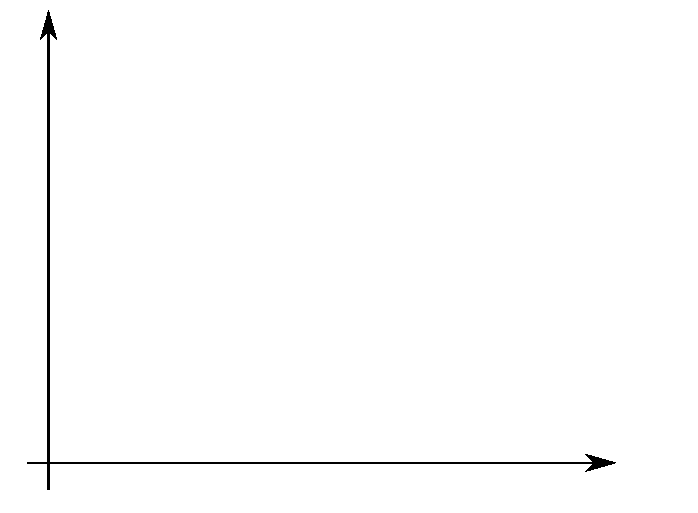
\includegraphics[width=0.85\textwidth]{figs/mobilerobot.png}
    \def\svgwidth{0.85\textwidth}
    \import{./figs/}{mobilerobot.pdf_tex}
    \caption{Mobile robot with local coordinate system \{R\} and world frame \{I\}. The arrows indicate the positive direction of position and orientation vectors.
    \td{Nikolaus: $\theta_i$ in this figure should point downwards right? }}
    \label{fig:mobilerobot}
\end{figure}



Notice that the positioning of the coordinate frames and their orientation are arbitrary. Here, we choose to place the coordinate system in the center of the robot's axle and align $^Rx$ with its default driving direction.
In order to calculate the robot's position in the inertial frame, we need to first find out how speed in the robot coordinate frame maps to speed in the inertial frame.
This can be done again by employing trigonometry. There is only one complication: a movement into the robot's $x-$axis might lead to movement along both the $x-$axis and the $y-$axis of the world coordinate frame ${I}$. By looking at \cref{fig:mobilerobot}, we can derive the following components to $\dot{x}_I$. First,
\begin{equation}
\dot{x}_{I,x}=cos(\theta) \dot{x}_R.
\end{equation}

There is also a component of motion coming from $ \dot{y}_R$ (ignoring the kinematic constraints for now, see below).  For negative $ \theta$, as in \cref{fig:mobilerobot}, a move along $y_R$ would let the robot move into positive $ X_I$ direction. The projection from $ \dot{y}_R$ is therefore given by
\begin{equation}
\dot{x_{I,y}}=-sin(\theta)\dot{y_R}.
\end{equation}
We can now write
\begin{equation}
\dot{x_I}=cos(\theta) \dot{x_R} - sin(\theta) \dot{y_R}.
\end{equation}
Similar reasoning leads to:
\begin{equation}
\dot{y_I}=sin(\theta) \dot{x_R} + cos(\theta) \dot{y_R}
\end{equation}
and
\begin{equation}
\dot{\theta_I}=\dot{\theta_R}
\end{equation}
which is the case because both robot's and world coordinate system share the same z-axis in this example. We can now conveniently write
\begin{equation}
\dot{\xi_I}=^I_RT(\theta)\dot{\xi_R}
\end{equation}
with
\begin{equation}
^I_RT(\theta)=\left[\begin{array}{ccc}
cos(\theta) & -sin(\theta) & 0 \\
sin(\theta) & cos(\theta) & 0 \\
0 & 0 & 1\end{array}\right]
\end{equation}

We are now left with the problem of how to calculate the speed $ \dot{\xi_R}$ in robot coordinates. For this, we make use of the \emph{kinematic constraints}\index{Kinematic constraints} of the robotic wheels.
For a standard wheel in an ideal case scenario, the kinematic constraints are that every rotation of the wheel leads to strictly forward or backward motion and does not allow side-way motion or sliding. We can therefore calculate the forward speed of a wheel $ \dot{x}$ using its rotational speed $ \dot{\phi}$ (assuming the encoder value/angle is expressed as $ \phi$) and radius $ r$ by
\begin{equation}
\dot{x}=\dot{\phi}r.
\end{equation}
This becomes apparent when considering that the circumference of a wheel with radius $r$ is $2\pi r$. The distance a wheel rolls when turned by the angle $ \phi$ (in radians) is therefore $ x=\phi r$, see also \cref{fig:wheelrotation}, right. Taking the derivative of this expression on both sides leads to the above expression.

\begin{figure}[htb!]
    \centering
    % 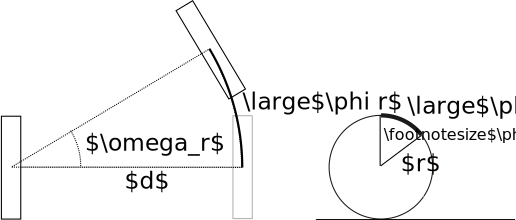
\includegraphics[width=0.9\textwidth]{figs/wheelrotation.png}
    \def\svgwidth{0.86\textwidth}
    \import{./figs/}{wheelrotation.pdf_tex}
    \caption{Left: Differential wheel robot pivoting around its left wheel. Right: A wheel with radius $r$ moves by $\phi r$ when rotated by $\phi$ degrees.}
    \label{fig:wheelrotation}
\end{figure}



How each of the two wheels in our example contributes to the speed of the robot's center---where its coordinate system is anchored---requires the following trick: we calculate the contribution of each individual wheel while assuming all other wheels remaining un-actuated.
In this example, the distance traveled by the center point is exactly half of that traveled by each individual wheel, assuming the non-actuated wheel rotating around its ground contact point (\cref{fig:wheelrotation}). We can therefore write:
\begin{equation}
\dot{x_R}=\frac{r\dot{\phi_l}}{2}+\frac{r\dot{\phi_r}}{2}
\end{equation}
given the speeds $ \dot{\phi_l}$ and $ \dot{\phi_r}$ of the left and the right wheel, respectively.

\begin{framed}
Think about how the robot's speed along its y-axis is affected by the wheel speed given the coordinate system in the drawing above. Think about the kinematic constraints that the standard wheels impose.
\end{framed}

Hard to believe at first, but the speed of the robot along its y-axis is always zero. This is because the constraints of the standard wheel tell us that the robot can never slide.
We are now left with calculating the rotation of the robot around its z-axis.
\td{This sentence is unclear: That there is such a thing can be immediately seen when imaging the robot's wheels spinning in opposite directions}.
We will again consider each wheel independently. Assuming the left wheel to be non-actuated, spinning the right wheel forwards will lead to counter-clockwise rotation. Given an axle diameter (distance between the robot's wheels) $d$, we can now write
\begin{equation}
\omega_r d = \phi_r r
\end{equation}
with $\omega_r$ the angle of rotation around the left wheel (\cref{fig:wheelrotation}, left). Taking the derivative on both sides yields speeds and we can write
\begin{equation}
\dot{\omega_r} = \frac{\dot{\phi_r} r}{d}
\end{equation}
Adding the rotation speeds up (with the one around the right wheel being negative based on the right-hand grip rule), leads to:
%
\begin{equation}
\dot{\theta}=\frac{\dot{\phi_r} r}{d}-\frac{\dot{\phi_l} r}{d}
\end{equation}
%
Putting it all together, we can finally write:

\begin{equation}\label{eq:diffwheels}
\left[\begin{array}{c} \dot{x_I}\\\dot{y_I}\\\dot{\theta}\end{array}\right]=\left[\begin{array}{ccc}
cos(\theta) & -sin(\theta) & 0 \\
sin(\theta) & cos(\theta) & 0 \\
0 & 0 & 1\end{array}\right]\left[\begin{array}{c}\frac{r\dot{\phi_l}}{2}+\frac{r\dot{\phi_r}}{2}\\0\\\frac{\dot{\phi_r} r}{d}-\frac{\dot{\phi_l} r}{d}\end{array}\right]
\end{equation}

\subsubsection{From Forward Kinematics to Odometry}

\cref{eq:diffwheels} only provides us with the relationship between the robot's wheel speed and its speed in the inertial frame.
Calculating its actual pose in the inertial frame is known as \emph{odometry}\index{Odometry}. Technically, it requires integrating \cref{eq:diffwheels} from 0 to the current time $T$.
As this is not possible but for very special cases, one can approximate the robot's pose by summing up speeds over discrete time intervals, or more precisely:
\begin{equation}
\left[\begin{array}{c} {x_I}(T)\\{y_I}(T)\\{\theta}(T)\end{array}\right]=
\int_0^T \left[\begin{array}{c} \dot{x_I}(t)\\\dot{y_I}(t)\\\dot{\theta}(t)\end{array}\right] dt \approx
\sum_{k=0}^{k=T}\left[\begin{array}{c} \Delta{x_I}(k)\\\Delta{y_I}(k)\\\Delta{\theta}(k)\end{array}\right]\Delta t
\end{equation} which can be calculated incrementally as
\begin{equation}\label{eq:odometry}
x_I(k+1)=x_I(k)+\Delta x (k) \Delta t
\end{equation}
using $\Delta x(k) \approx \dot{x_I}(t)$ and similar expressions for $y_I$ and $\theta$. Note that \cref{eq:odometry} is just an approximation. The larger $\Delta t$ becomes, the more inaccurate this approximation becomes as the robot's speed might change during the interval.

\begin{framed}
\noindent Don't let the notion of an integral worry you! As robots' computers are fundamentally discrete, integrals usually turn into sums, which are nothing than for-loops.
\end{framed}

\subsection{Forward kinematics of Car-like steering}\label{sec:kinematics:carsteering}

Differential wheel drives are very popular in mobile robotics as they are very easy to build, maintain, and control.
Although not holonomic, a differential drive can approximate the function of a fully holonomic robot by first driving on the spot to achieve the desired heading and then driving straight.
Drawbacks of the differential drive are its reliance on a caster wheel, which performs poorly at high speeds, and difficulties in driving straight lines as this requires both motors to drive at the exact same speed.

These drawbacks are mitigated by car-like mechanisms, which are driven by a single motor and can steer their front wheels. This mechanism is known as ``Ackermann steering''. \index{Ackermann steering}
Ackermann steering should not be confused with ``turntable'' steering \index{Turntable steering} where the front wheels are fixed on an axis with central pivot point.
Instead, each wheel has its own pivot point and the system is constrained in such a way that all wheels of the car drive on circles with a common center point, avoiding skid.
As the Ackermann mechanism lets all wheels drive on circles with a common center point, its kinematics can be approximated by those of a tricycle with rear-wheel drive, or even simpler by a bicycle. This is shown in \cref{fig:ackermann}.

\begin{figure}[htb!]
    \centering
    % 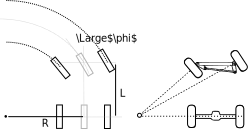
\includegraphics[width=0.9\textwidth]{figs/ackermann.png}
    \def\svgwidth{0.9\textwidth}
    \import{./figs/}{ackermann.pdf_tex}
    \caption{Left: Kinematics of car-like steering and the equivalent bicycle model. Right: Mechanism of an Ackermann vehicle.}
    \label{fig:ackermann}
\end{figure}

Let the car have the shape of a box with length $L$ between rear and front axis. Let the center point of the common circle described by all wheels be distance $ R$ from the car's longitudinal center line.  Then, the steering angle $ \phi$ is given by

\begin{equation}\label{eq:ackermann}
\tan \phi = \frac{L}{R}
\end{equation}

The angles of the left and the right wheel, $ \phi_l$ and $ \phi_r$ can be calculated using the fact that all wheels of the car rotate around circles with a common center point. With the distance between the two front wheels $l$, we can write:
\begin{eqnarray}
\frac{L}{R-l/2}&=\tan{(\phi_r)} \nonumber \\
\frac{L}{R+l/2}&=\tan{(\phi_l)}
\end{eqnarray}
This is important, as it allows us to calculate the resulting wheel angles resulting from a specific angle $\phi$ and test whether they are within the constraints of the actual vehicle.

Assuming the wheel speed to be $\dot{\omega}$ and the wheel radius $r$, we can calculate the speeds in the robot's coordinate frame as:
\begin{eqnarray}
\dot{x}_r&=\dot{\omega}r \nonumber \\
\dot{y}_r&=0\\
\dot{\theta}_r&=\frac{\dot{\omega}r\tan\phi}{L} \nonumber
\end{eqnarray}
using (\ref{eq:ackermann}) to calculate the circle radius $R$.

\subsection{The Denavit-Hartenberg notation}\label{sec:kinematics:dh}

So far, we have considered the forward kinematics of wheeled mechanisms and simple arms and derived relationships between actuator parameters and velocities using basic trigonometry.
In the case of multi-link arms (which is the vast majority of robot manipulators in existence), the approach detailed in \cref{sec:kinematics:fwkarm} is difficult to scale, and alternative solutions are needed.
Interestingly, we can think of the forward kinematics as a chain of homogeneous transformations with respect to a coordinate system mounted at the base of a manipulator or a fixed position in the room.
Deriving these transformations can be confusing and can be facilitated by following a ``recipe'' such as the one conceived by Denavit and Hartenberg in $1955$ \td{citation?}.
The so-called Denavit-Hartenberg (DH)\index{Denavit-Hartenberg parameters} representation has evolved as a \textsl{de-facto} standard and can easily be automatized, i.e., applied to a 3D model of a robotic arm, e.g. \td{Nikolaus, what do you meant here?}

A manipulator consists of a series of typically rigid links that are connected by joints.
In the vast majority of cases, a joint can either be revolute (i.e. change its angle/orientation) or prismatic (i.e. change its length).
Knowing the robot's kinematic properties (e.g. the length of all rigid links, similarly to $l_1$ and $l_2$ in \cref{fig:fwk2dofarm}), the pose of its end-effector is fully described by its joint configuration (angle for revolute joints, length for prismatic joints).

%In industrial manipulators, the number of joints is usually equal to the degrees of freedom of the manipulator. As most manipulators are holonomic, the forward kinematics allow you---unlike on non-holonomic wheeled platforms---to directly relate absolute positions of joints with absolute positions in Cartesian space. It is also possible to derive equations that relate the speed of the joints to speed in Cartesian space. Like for wheeled platforms, this can be achieved via a Jacobian matrix.  At certain positions, the mapping provided by the Jacobian is not invertible, i.e., some velocities in Cartesian space are unachievable. These points are called singularities.

\screencast{http://youtu.be/rA9tm0gTln8}{denavithartenberg}

\begin{figure}[!t]
    \centering
    % 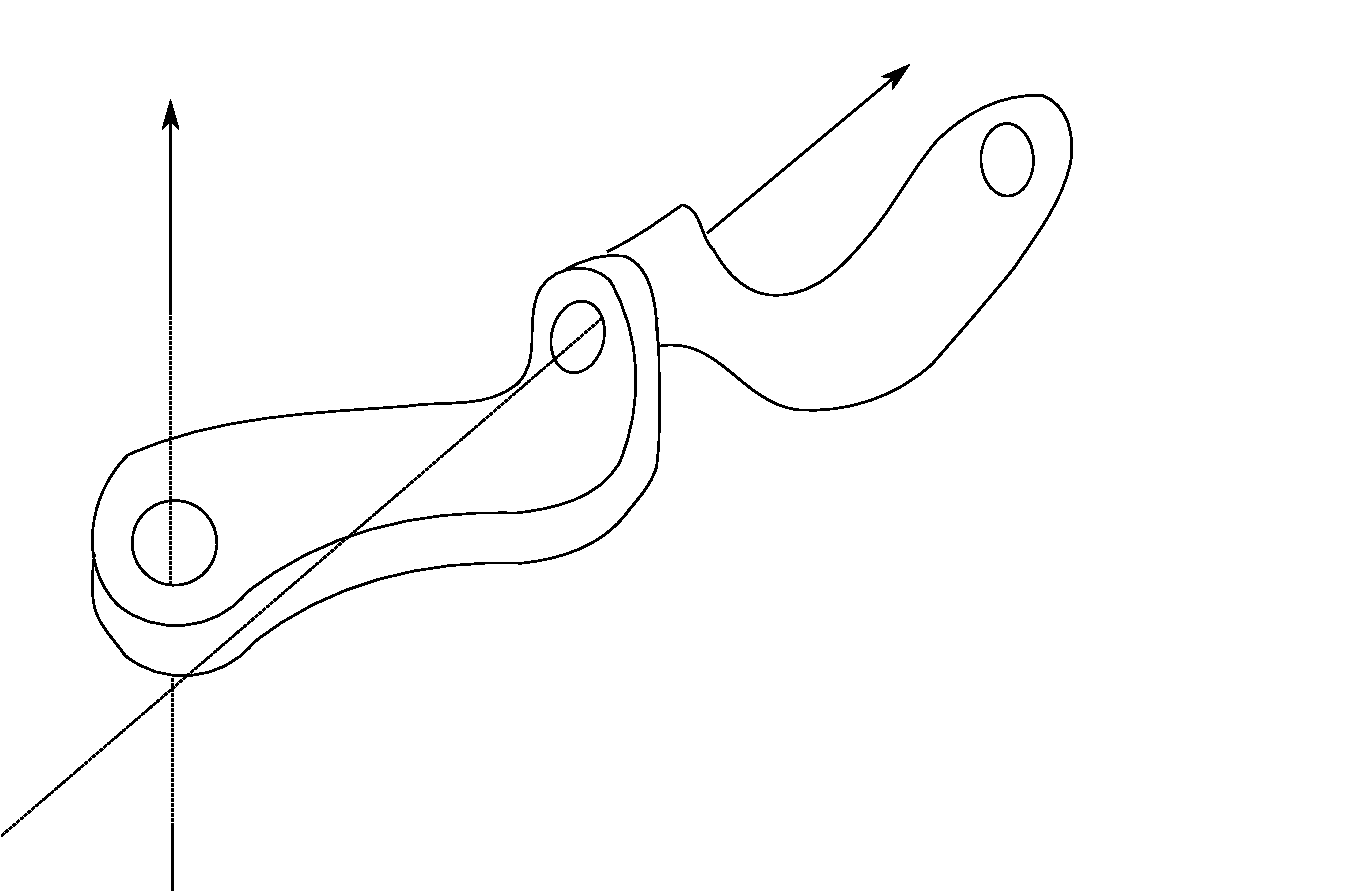
\includegraphics[width=\textwidth]{figs/denavit-hartenberg.png}
    \def\svgwidth{\textwidth}
    \import{./figs/}{denavit-hartenberg.pdf_tex}
    \caption{Example of selected Denavit-Hartenberg parameters for three sequential revolute joints. The z-axes of joint $i$ and $i+1$ are parallel.}
    \label{fig:denavit}
\end{figure}

In order to use the DH-convention, we first need to define a coordinate system at each joint. With reference to \cref{fig:denavit}, we choose the $z-$axis to be the axis of rotation for a revolute joint and the axis of translation for a prismatic joint.
We can now find the common normal between the $z-$axes of two subsequent joints, i.e. a line that is orthogonal to each $z-$axis and intersects both.
With the direction of the $x-$axis at the base arbitrary, subsequent $x-$axes are chosen such that they lie on the common normal shared between two joints.
Whereas the direction of the $z-$axis is given by the positive direction of rotation (right-hand rule), the $x-$axis points away from the previous joint.
This allows defining the $y-$axis using the right-hand rule.
Note that these rules, in particular the requirement that $x$-axes lie along the commom normal, might result in coordinate systems with their origins outside the joint: this is not relevant as the kinematics of a manipulator is a mathematical representation that needs to represent the geometric and kinematic properties of the robot, and does not need to bear any physical correspondence.
%
The transformation between two joints is then fully described by the following four parameters:
\begin{enumerate}
\item The length $r$ (sometimes, $a$ is used) of the common normal between the $z$-axes of two joints $i$ and $i-1$ (link length).
\item The angle $ \alpha$ between the z-axes of the two joints with respect to the common normal (link twist), i.e. the angle between the old and the new $z$-axis, measured about the common normal.
\item The distance $d$ between the joint axes (link offset), i.e. the offset along the previous $z$-axis to the common normal.
\item The rotation $ \theta$ around the common axis along which the link offset is measured (joint angle), i.e. the angle from the old $x$-axis to the new $x$-axis, about the previous $z$-axis.
\end{enumerate}

Two of the above D-H parameters describe the link between the joints, and the other two describe the link's connection to a neighboring link.
Depending on the link/joint type, these numbers are fixed by the specific mechanical instance of the robot or can be controlled.
For example, in a revolute joint $ \theta$ is the varying joint angle, while all other quantities are fixed.  Similarly, for a prismatic joint $d$ is the joint variable. An example of two revolute joints is shown in \cref{fig:denavit}.

The final coordinate transform from one link ($i-1$) to another ($i$) can now be constructed by concatenating the four steps above, which are nothing but a series of rotations and translations, one for each DH parameter:
%
\begin{equation}\label{eq:kinematics:dh:composition}
_{n-1}^nT=T_z'(d_n) R_z'(\theta_n) T_x(r_n)  R_x(\alpha_n)
\end{equation}
with
\begin{equation}
T_z'(d_n)=
\left[
\begin{array}{ccc|c}
1 & 0 & 0 & 0\\
0 & 1 & 0 & 0\\
0 & 0 & 1 & d_n\\
\hline
0 & 0 & 0 & 1
\end{array}
\right]
\enskip
R_z'(\theta_n)=\left[
\begin{array}{ccc|c}
\cos\theta_n & -\sin\theta_n & 0 & 0\\
\sin\theta_n & \cos\theta_n & 0 & 0\\
0 & 0 & 1 & 0\\
\hline
0 & 0 & 0 & 1
\end{array}
\right]
\end{equation}
and
\begin{equation}
T_x(r_n)=
\left[
\begin{array}{ccc|c}
1 & 0 & 0 & r_n\\
0 & 1 & 0 & 0\\
0 & 0 & 1 & 0\\
\hline
0 & 0 & 0 & 1
\end{array}
\right]
\enskip
R_x(\alpha_n)=\left[
\begin{array}{ccc|c}
1 & 0 & 0 & 0\\
0 & \cos\alpha_n & -\sin\alpha_n & 0\\
0 & \sin\alpha_n & \cos\alpha_n & 0\\
\hline
0 & 0 & 0 & 1
\end{array}
\right]
\end{equation}
%
These are a translation of $d_n$ along the previous z-axis ($T_z'(d_n)$), a rotation of $\theta_n$ about the previous z-axis ($R_z'(\theta_n)$), a translation of $r_n$ along the new $x$-axis ($T_x(r_n)$)and a rotation of $\alpha_n$ around the new $x$-axis ($R_x(\alpha_n)$).
%
By replacing each element in \cref{eq:kinematics:dh:composition}, the following matrix is created:
\begin{eqnarray}
_{n-1}^nT&=
\left[
\begin{array}{ccc|c}
\cos \theta_n & -\sin \theta_n \cos\alpha_n & \sin\theta_n \sin\alpha_n & r_n \cos\theta_n\\
\sin \theta_n & \cos\theta_n \cos\alpha_n & -\cos\theta_n\sin\alpha_n & r_n \sin\theta_n\\
0 & \sin\alpha_n & \cos\alpha_n & d_n \nonumber \\
\hline
0 & 0 & 0 & 1
\end{array}
\right]\\
&=
\left[
\begin{array}{c|c}
R & t\\
\hline
0 \quad 0 \quad 0 & 1
\end{array}
\right]
\end{eqnarray}
where $R$ is the $3\times3$ rotation matrix and $t$ is the $3\times1$ translation vector.

Like for any homogeneous transform, the inverse $_{n-1}^nT^{-1}n$ is given by
\begin{equation}
^{n-1}_nT=\left[
\begin{array}{c|c}
R^{-1} & -R^{-1}T\\
\hline
0 \quad 0 \quad 0 \quad 1
\end{array}
\right]
\end{equation}
with the inverse of $R$ simply being its transpose, $R^{-1}=R^T$.

Similar to the concatenation of transformations detailed in \cref{sec:kinematics:coordsystems:concatenation}, $_{n-1}^nT$ in \cref{eq:kinematics:dh:composition} can be concatenated with the other transformation matrices relative to the remaining links in order to compute a the full kinematics of the robot arm from the base reference frame up to the end-effector.

%!TEX root = ../book.tex
\section{Inverse Kinematics}\label{sec:kinematics:ik}

The forward kinematics of a system are computed by means of a transformation matrix from the base of a manipulator (or fixed location, such as the corner of a room) to the end-effector of a manipulator (or a mobile robot).
As such, they are an exact description of the pose of the robot and they fully characterize its kinematic state.
Inverse Kinematics deal with the opposite problem: finding a joint configuration that results in a desired pose at the end effector.
To achieve this goal, we will need to solve the forward kinematics equations for joint angles as a function of the desired pose.
With reference to \cref{eq:kinematics:forward}, inverse kinematics aims to solve the following:
\begin{equation}\label{eq:kinematics:inverse}
q = f^{-1} (r)\ , \qquad f^{-1} : \mathbb{R}^m \rightarrow \mathbb{R}^n \ ,
\end{equation}
with a notation similar to \cref{eq:kinematics:forward}.
For a mobile robot, we can do this only for velocities in the local coordinate system, and need more sophisticated methods to calculate appropriate trajectories. We will discuss this in depth in \cref{sec:kinematics:diff}.

\subsection{Solvability}

\cref{eq:kinematics:inverse} is the inverted version of \cref{eq:kinematics:forward}, and is heavily non-linear except for trivial mechanisms.
Therefore, it makes sense to briefly think about whether we can solve it at all for specific parameters before trying.
Here, the workspace of a robot becomes important. The workspace is the sub-space that can be reached by the robot in any configuration.
Clearly, there will be no solutions for the inverse kinematic problem outside of the workspace of the robot.

A second question to ask is how many solutions we actually expect to exist and what it means to have multiple solutions \textsl{geometrically}.
Multiple solutions to achieve a desired pose correspond to multiple ways in which a robot can reach a target (i.e., joint configurations).
For example a three-link arm that wants to reach a point that can be reached without fully extending all links (which would have only a single solution) can do this by either folding its links in a concave or a convex fashion.
Reasoning about how many solutions will exist for a given mechanism and desired pose quickly becomes non-intuitive.
For example, a 6-DOF arm can reach certain points with up to $16$ different configurations!

\subsection{Inverse Kinematics of a Simple Manipulator Arm}\label{sec:kinematics:inverse:arm}

We will now look at the inverse kinematics of the $2-$link arm that we introduced in \cref{fig:fwk2dofarm}. We need to solve the equations determining the robot's forward kinematics by solving for $\alpha$ and $ \beta$.
This is tricky, however, as we have to deal with more complicated trigonometric expressions than the forward kinematics case.

To build an intuition, assume there to be only one link, $l_1$.  Solving (\ref{eq:cosxl1}) for $\alpha$ yields to two distinct solutions:

\begin{equation}
\alpha = \pm \cos^{-1}\frac{x_1}{l_1},
\end{equation}
as cosine is symmetric for positive and negative values.
Indeed, for any possible position on the $x-$axis ranging from $-l_1$ to $l_1$, there exist two solutions: the first one with the arm above the table, and the other one with the arm below it.
At the extremes of the workspace, both solutions are the same.

%\begin{verbatim}
%sol = Solve[Sin[a + b] + Sin[a] == y
%             && Cos[a + b] + Cos[a] == x,
%            {a, b}];
%min = sol /. {x -> 1, y -> 1}
%\end{verbatim}

Solving \ref{eq:fwk2dofarm} for $\alpha$ and $\beta$ adds two additional solutions that are cumbersome to reproduce here, involving terms of $x$ and $y$ to the sixth power, and is left as an exercise to the reader, for example using an online symbolic solver.


What will drastically simplify this problem, is to not only specify the desired position, but also the orientation $\theta$ of the end-effector. In this case, a desired pose can be specified in the following form
\begin{equation}
\left[
\begin{array}{cccc}
cos\theta & -sin\theta & 0 & x\\
sin\theta & cos\theta & 0 & y\\
0 & 0 & 1 & 0\\
0 & 0 & 0 & 1
\end{array}
\right].
\end{equation}
A solution can now be found by simply equating the individual entries of the transformation (\ref{eq:2armtrans}) with those of the desired pose. Specifically, we can observe:
\begin{eqnarray}
cos\theta &=& cos(\alpha+\beta)\\
\nonumber
x &=& c_{\alpha\beta}l_2+c_\alpha l_1\\
\nonumber
y &=& s_{\alpha\beta}l_2+s_\alpha l_1
\end{eqnarray}
These can be reduced to
\begin{eqnarray}
\theta &=& \alpha + \beta \nonumber \\
c_\alpha &=& \frac{c_{\alpha\beta}l_2-x}{l_1}=\frac{c_\theta l_2-x}{l_1} \\
s_\alpha &=& \frac{s_{\alpha\beta}l_2-y}{l_1}=\frac{s_\theta l_2-y}{l_1} \nonumber
\end{eqnarray}
Providing the orientation of the robot in addition to the desired position therefore allows solving for $\alpha$ and $\beta$ just as a function of $x$, $y$ and $\theta$.

The main issue with the geometric approach detailed above is that it does not scale easily with an increase of DoF at the joints, and it quickly becomes unwieldy with more dimensions.
For higher-DoF platforms, we can calculate a \textsl{numerical solution} using an approach that we will later see is very similar to path planning in mobile robotics.
To this end, we will take an optimization-based approach: first we calculate a measure of error between the current solution and the desired one, and then change the joint configuration in a way that minimizes this error.
In our example, the measure of error is the Euclidean distance between the current end-effector pose (given by the forward kinematics equations in \cref{eq:fwk2dofarm}) and the desired solution $[x,y]$ in configuration space, i.e. (assuming $l_1=l_2=1$ for simplicity):
% To do this, you need to solve the forward kinematics for every point in configuration space and use the Euclidean distance to the desired target as height.
\begin{equation}\label{eq:kinematics:inverse:numerical}
f_{x,y}(\alpha,\beta)=\sqrt{\left(s_{\alpha\beta} + s_\alpha - y\right)^2 + \left(c_{\alpha\beta}+c_\alpha - x\right)^2}
\end{equation}
Here, the first two terms in parentheses are given by the forward kinematics of the robot, whereas the third term in the parentheses is the desired $y$ and $x$ position, respectively.
\cref{eq:kinematics:inverse:numerical} can be plotted as a 3D function of $\alpha$ and $\beta$, our joint-space variables.
% This is plotted for $\alpha=[-\pi/2,\pi/2]$ and $\beta=[-\pi,\pi]$ and $x=1$, $y=1$ in Figure~\ref{fig:inversekinematics}.
As shown in \cref{fig:inversekinematics} this function has a minima, in this case zero, for values of $\alpha$ and $\beta$ that bring the manipulator to $(1,1)$. These values are $(\alpha \rightarrow 0, b \rightarrow -\frac{\pi}{2})$ and $(\alpha \rightarrow -\frac{\pi}{2}, b \rightarrow \frac{\pi}{2})$.

\begin{figure}
    \centering
        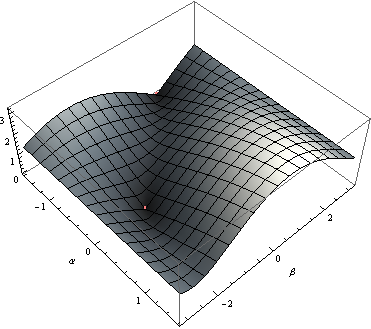
\includegraphics[width=0.8\textwidth]{figs/kinematics/inversekinematics}
    \caption{Distance to $(x=1,y=1)$ over the configuration space of a two-arm manipulator. Minima corresponds to exact inverse kinematic solutions.}
    \label{fig:inversekinematics}
\end{figure}

You can now think about inverse kinematics as a path finding problem from anywhere in the configuration space to the nearest minima. A more formalized approach to this will be discussed in \cref{sec:kinematics:inverse:feedbackcontrol}. How to find the shortest path in space, that is finding the shortest route for a robot to get from A to B, is one of the subjects covered within \cref{chap:pathplanning}.




%%%%%%%%%%%%%%%%%%%%

\section*{Take-home lessons}

\begin{itemize}
\item Forward kinematics are equivalent to finding a coordinate transform from a world coordinate system into a coordinate system on the robot. Such a transform is a combination of a (3x1) translation vector and a (3x3) rotation matrix that consists of the unit vectors of the robot coordinate system. Both translation and rotation can be combined into a 4x4 homogeneous transform matrix.
\item Forward and Inverse Kinematics of a mobile robot are performed with respect to the speed of the robot and not its position.
\item For calculating the effect of each wheel on the speed of the robot, you need to consider the contribution of each wheel independently.
\item Calculating the inverse kinematics analytically becomes quickly infeasible. You can then plan in configuration space of the robot using path-planning techniques.
\item The inverse kinematics of a robot involves solving the equations for the forward kinematics for the joint angles. This process is often cumbersome if not impossible for complicated mechanisms.
\item A simple numerical solution is provided by taking all partial derivatives of the forward kinematics in order to get an easily invertible expression that relates joint speeds to end-effector speeds.
The inverse kinematics problem can then be formulated as feedback control problem, which will move the end-effector towards its desired pose using small steps. Problems with this approach are local minima and singularities of the mechanism, which might render this solution infeasible.
\end{itemize}

\section*{Exercises}\small
\subsection*{Coordinate systems}
\begin{enumerate}
\item
\begin{enumerate}
 \item Write out the entries of a rotation matrix $^A_BR$ assuming basis vectors $X_A$, $Y_A$, $Z_A$, and $X_B$, $Y_B$, $Z_B$.
 \item Write out the entries of rotation matrix $^B_AR$.
 \end{enumerate}
\item Assume two coordinate systems that are co-located in the same origin, but rotated around the z-axis by the angle $\alpha$. Derive the rotation matrix from one coordinate system into the other and verify that each entry of this matrix is indeed the scalar product of each basis vector of one coordinate system with every other basis vector in the second coordinate system.
\item Consider two coordinate systems $\{B\}$ and $\{C\}$, whose orientation is given by the rotation matrix $^C_BR$ and have distance $^BP$. Provide the homogenous transform $^C_BT$ and its inverse $^B_CT$.
\item Consider the frame $\{B\}$ that is defined with respect to frame $\{A\}$ as $\{B\}=\{^A_BR, ^AP\}$. Provide a homogeneous transform from $\{A\}$ to $\{B\}$.
\item Program a simple application that displays a 2D (or 3D) coordinate system and add the ability to move and turn the coordinate system using your keyboard.
\end{enumerate}

\subsection*{Forward and inverse kinematics}
\begin{enumerate}
\item Consider a differential wheel robot with a broken motor, i.e., one of the wheels cannot be actuated anymore. Derive the forward kinematics of this platform. Assume the right motor is broken.
\item Consider a tri-cycle with two independent standard wheels in the rear and the steerable, driven front-wheel. Choose a suitable coordinate system and use $\phi$ as the steering wheel angle and wheel-speed $\dot{\omega}$. Provide forward and inverse kinematics.
\item Program an application that displays a differential wheel platform and allows you to control forward and rotational speed with your keyboard. Output the robot's pose after every step.
\item Program an application that display a two-link robotic arm moving in the plane and lets you change both joint angles using your keyboard.
\item Derive the forward kinematics of a two-link robotic arm as well as its Jacobian. Implement its inverse kinematic using the inverse Jacobian technique.
\item Program an application that displays a two-link robotic arm moving in the plane and lets you change the position of its end-effector using your keyboard.
\item Explore the internet for toolkits that allow you to manage forward and inverse kinematics for a robotic arm. What kind of tools do you find and what kind of input do they require to model the robot's geometry?
\item Download the manual of a commercially available robot arm of your choice. What kind of input does it take from its user? Does it allow you to control its position directly?
\item Use a robot simulator of your choice to access a simulated vehicle. What kind of actuator input can you provide and what are the sensors that are available? Drive the car using your keyboard and try to estimate its pose by implementing odometry.
\end{enumerate}
\normalsize


%!TEX root = ../book.tex
\chapter{Forces}\label{ch:forces}
%alessandro

So far, we have only been concerned with how robots move and the \textsl{geometry of motion}.
However, moving a robot not only requires a kinematic model of the platforms, but also an understanding of the forces needed to move the robot and interact with the environment.
While this aspect can be ignored in basic applications of mobile robots and simple manipulation, it becomes critical as soon as robots interact more closely with people or need to engage in more complex manipulation.

%The (geometric) Jacobian represents a fundamental tool to characterize the motion and the interaction of a robot with its environment, as it is used to perform the following \cite{sciavicco2012modelling}):
%\begin{enumerate}
%\item inverse differential kinematics even for robots that do not have a closed-form solution (\cref{sec:invjac});
%\item singularity analysis (a kinematic singularity is a robot configuration in which the robot loses the ability to move to one or more directions);
%\item redundancy analysis (a kinematic task is redundant if the robot possesses more degrees of freedom than what are needed to perform the task, resulting in infinite inverse kinematics solutions to choose from);
%\item manipulability analysis (i.e. how easy or difficult is it for a robot to move in a certain direction).
%\end{enumerate}
In this Chapter, we will introduce the reader to the concept of \emph{Statics}\index{Statics}, which introduces a third dimension to the problem of analyzing how robots move in space and interact with their surroundings.
More specifically, in \cref{sec:kinematics:fwk,sec:kinematics:ik} we have investigated the \textsl{kinematic} problem and operated in the space of \textsl{positions}, that is, how to map joint angles with end effector poses.
In \cref{sec:kinematics:ik:invjac}, we introduced the \textsl{differential kinematics} problem and operated in the space of \textsl{velocities}, i.e. how to map joint velocities with end-effector velocity screws (remember: velocity is derivative of position, hence the name ``differential'').
In the following, we will operate in the space of \textsl{forces}; however, we will simplify the more general dynamical problem by looking at the robot in equilibrium---otherwise known as a \textsl{static} configuration.
As we will see, a lot can be done by simply looking at the robot in an equilibrium configuration!
The last dimension, which goes beyond the scope of this book, is called \textsl{dynamics} and operates in the space of forces from a non-static perspective; it involves the second derivative of position (i.e. the acceleration), and is a generalization of the second law of Newton ($F=ma$).
We will briefly introduce the reader to the topic in \cref{ch:forces:dynamics}.\td{remember to remove this sentence if we decide not to have the subchapter on dynamics}
%
The goals of this chapter are to:

\begin{itemize}
\item introduce the concept of statics
\item understand the so called kineto-statics duality
\item \td{finish thiswhen the chapter is finished}
\item briefly introduce the dynamics problem.
\end{itemize}


\begin{mdframed}
\noindent The analysis of motion of a robot can be thought as a layered system with multiple levels of abstraction of increasing complexity.
The more complex it becomes, the more comprehensive your analysis will be, and the more capability you will be able to squeeze out of the robot!
However, it is good practice to start with the simplest layer first (i.e. kinematics), and gradually progress toward a dynamic analysis only if needed.
\end{mdframed}

\section{Statics}

In this Chapter, we will investigate the role of the Jacobian in relating joint torques $\tau$ with forces and moments $[f \ m]^T$ applied at the end-effector--and we are going to do all of this in equilibrium (or \textsl{static}) configurations.


The Jacobian formulation introduced in \cref{sec:invjac} pertains to the field known as \emph{Differential Kinematics}, which relates joint velocities $\dot{q}$ with end-effector linear and angular velocities (i.e. the velocity screw $[v \ \omega]^T$).


  deals with relating forces at the end-effector and generalized forces at the robot joints---either torques for revolute joints or forces for prismatic joints---when the robot is in \emph{static equilibrium}, i.e. the acceleration of the robot and all of its components is zero
(for simplicity, we will hereinafter refer to robot manipulators equipped with revolute joints unless otherwise specified).
If such a condition is met, a robot with $n$ degrees of freedom and an end-effector characterized by $m$ degrees of freedom can be fully described by the following quantities:
\begin{itemize}
    \item an $\left( n \times 1 \right)$ vector of joint torques $\tau$;
    \item an $\left( m \times 1 \right)$ vector of \textbf{equivalent} forces exerted at the robot end-effector $F$;
    \item an $\left( m \times 1 \right)$ vector of forces exerted \textbf{by the environment} on the robot end-effector $F_e$--which, per the principle of action and reaction, are equal and opposite to $F$: $F_e=-F$.
\end{itemize}

\td{finish}
\vskip 40pt
\ar{here's what I will cover:}

\section{Kineto-statics Duality}

\section{Manipulability}

\section{Dynamics}\label{ch:forces:dynamics}


\section*{Take-home lessons}

\section*{Exercises}\small

\begin{enumerate}
\item Think about the four layer of abstraction we have just investigated (kinematics, differential kinematics, statics, dynamics).
\begin{enumerate}
\item Can you think of an application for which you would need a dynamic analysis? (Hint: this is generally something really hard)
\item What can be done by just looking at the static problem instead? (Hint: you are still considering an exchange of forces here)
\item What can you do with a robot from a purely kinematic perspective? (Hint: this is typically easy)
\end{enumerate}
\end{enumerate}

\chapter{Grasping}
Grasping is the activity in which the robot extends its body by attaching an external object to its kinematic chain. This allows the robot to move this object and potentially manipulate it, that is change its shape or pose. Grasping has the interesting, and very confusing, property that its relatively easy in practice, but very difficult in theory. In particular, this chapter is able to describe a variety of strategies that will lead to successful grasps for a wide range of objects, but has difficulties to answer questions such as \emph{What makes a good grasp?} or \emph{How to find good grasps?} in any more depth than by providing simple heuristics.

\section{The theory of grasping}
The theory of grasping is quite involved, with the state of the art comprehensively described in \cite{rimon2019mechanics}, yet has difficulties to mathematically exactly capture the mechanics of grasping mechanisms that are successful in practice. Rather than describing these developments here --- which will be well beyond the scope of this book --- we will briefly describe different approaches to model grasping, and there limitations, to provide an understanding of what the reasons for grasps that work.

\subsection{Friction}\index{Friction}
In its most simple form, grasping requires immobilizing an object, at least agains the forces of gravity, by providing appropriate forces in the opposite direction. Specifically, contact points on a robotic finger, gripper or hand are assumed to exert localized forces, thereby constraining the object sufficiently. By this, fingers act essentially as miniature robotic arms, allowing us to apply the methods and tools from previous chapters~\ref{chap:locomotion}--\ref{ch:forces}.

%% DRAWING OF TWO FINGERS HOLDING AN OBJECT WITH TWO FINGERS AND WITH THREE FINGERS. SHOW COORDINATE SYSTEM.
\begin{figure}
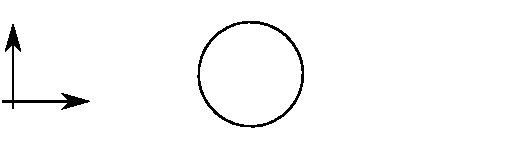
\includegraphics[width=\columnwidth]{figs/idealgrasp}
\caption{Cross-section from above showing an idealized two-finger (left) and three finger (right) gripper holding a cylinder.\label{fig:idealgrasp}.}
\end{figure}

While already very involved for anything but very simple mechanisms, such a model only captures a very small slice of realistic grasps. In any real application, contacts between a gripper and hand are not friction-less. This is the reason a grasp such as shown in Figure~\ref{fig:idealgrasp} actually works. If there were really no friction between the fingers and the object, the object would be ejected from the hand for every grasp that is not exactly aligned with a principal axis of the cylinder in Figure~\ref{fig:idealgrasp}, left. Furthermore, even the three-finger grasp shown in  Figure~\ref{fig:idealgrasp}, right, would \emph{always} fail as there is no force constraining the object from below. Fortunately, the existance of friction makes grasping much easier in practice, yet much harder to describe mathematically.

The reason that the grasps shown in Figure~\ref{fig:idealgrasp} do work in most circumstances is that the normal forces shown have a tangential component that is due to friction and covered by \emph{Coloumb's Friction law,}\index{Coloumb Friction}

which states that the higher the friction coefficient of a material, the more normal force translates into tangential forces that can resist two surfaces from moving against each other:

It is governed by the equation:
\begin{equation}
F_\mathrm{t} \leq \mu F_\mathrm{n}.
\end{equation}

Here $F_\mathrm{t}$  is the force of friction exerted by each surface on the other and $F_\mathrm{n}$ is the normal force. The force $F_\mathrm{t}$ acts in tangential direction of the normal force applied by, e.g., a finger's tip, where $\mu$ is an empirical coefficient of friction.

The friction coefficient $\mu$ is low for glass on glass and high for rubber on wood.  We are therefore interested in designing grippers with high friction coefficients to avoid objects from slipping.

When do objects slip? Lets say we have a fingertip pressing down on a surface in any orientation. There will be a force normal to the surface $F_\mathrm{n}$, which defines the tangential force $F_\mathrm{t}$ in any direction. Sweeping the tangential force around the normal force creates a cone with an opening angle of
\begin{equation}
\alpha=2tan^{-1}\mu,
\end{equation}
see \cite[p. 57]{rimon2019mechanics} for a derivation.
If the net force on the object is not within this cone, the object slips.  This becomes more intuitive when thinking about how different values of $\mu$ affect the shape of this cone. If $\mu$ is high, the cone will be relatively flat, letting the object accept forces from many different directions without slipping. If $\mu$ is low, the cone will be relatively narrow, requiring the force to be normal to the object's surface to prevent slippage.

\begin{figure}
\caption{Left: Coloumb friction relates normal to tangential reaction forces that are required to overcome friction, here shown for rightwards motion. Right: Friction cone for point forces. As long as the force is within the cone cone, the finger will not slip.}
\end{figure}
%% FIGURE SHOWING THE FRICTION CONE

A force applied to a rigid body will exert both a force as well as a torque to the body's center of gravity. This is called a \emph{wrench}\index{Wrench}. If we consider the possible forces that we can apply to a rigid body without having the end-effector slip to form a space (namely the cone described earlier), we can talk about the \emph{grasping wrench space}\index{Grasping wrench space}, which is the corresponding space of all suitable wrenches.

Knowing the relation between normal and tangential reaction forces can help in designing grippers that are more likely to successfully grasp an object than others, as well as when planning suitable grasp for objects with known friction.

%In summary: we can use Coloumb's law of friction to determine the direction of forces that we can apply to a certain contact point without that the object slips. These forces translate into wrenches to the object's center of gravity. A grasp fits a certain task if the wrenches that would fulfill the task can be effectuated without slip. The less force is waisted to overcome slip, the better is the grasp.

\subsection{Multiple contacts and deformation}
In practice, no force will ever be applied at a single point only, but over an area, either due to the size of the finger pad itself or due to the contact area deforming. Even the smallest contact area will allow to not only additional force constraints, but also constraints on torque, thereby adding constraints in additional dimensions and therefore further stabilizing the grasp. This is illustrated in Figure~\ref{fig:contactarea}. Whereas the object can easily pivot around the point of contact in Figure~\ref{fig:contactarea}, left, increasing the area of contact only slighlty constrains the rotational degree of freedom. It is therefore desirable to grasp an object with an as large contact area as possible. (A large contact area will also increase friction.)

\begin{figure}
\caption{From left to right: ideal force exerted via a single point of contact, forces exerted via an area of contact, contact area increasing due to pressure and conforming with the surface.\label{fig:contactarea}}
\end{figure}

A perfectly flat surface has only a single point of contact when grasping a cylinder or sphere. Indeed, using blank metal grippers or fingers is little successful in practice. Instead, rubber pads are used to increase force closure by conforming around the object. As the rubber is flexible, however, the grasp is not completely fixating the object, but it can move within the grasp, which might not be desirable when picking up a nut, e.g., and trying to mount it on a screw.

\subsection{Suction}

A highly capable method for grasping is using suction. Here, a suction cup is pressed against an object, using a vacuum applied by a pump to suck the object against the cup. Instead of exerting forces against the object, which always requires at least one antipodal force (or multiple forces that are distributed such that the object remains in equilibrium), suction only requires one point of contact. The rim of the suction cup provides both friction, to prevent the object to slip, and multiple contact points that further constrain the object beyond the normal force applied by the vacuum. The soft nature of the suction cup provides the ability for the rim to conform to the object, ruling out objects that do not have any flat surfaces. The elasticity of the rim also makes it difficult to further manipulate the object as all forces applied by the robot will need to be transferred via a spring-like elastic material.

\subsection{Non-prehensile manipulation}

\section{Simple grasping mechanisms}

\subsection{1-DoF gripper}
-Example: Utah prosthetic hand
-Strategy: make contact with stiff part until contact is made (touch sensor or wrist force), then close gripper

\subsection{Parallel jaw}
-Most industrial robotic grippers
-Simple kinematics, single motor
-Worm gear drive is slow, range is limited by width of the gripper

\subsection{4-bar linkage}
- Some industrial robotic grippers
- more complex kinematics, single or dual motor
- having two motors can be advantageous, in particular in conjunction with torque control

\subsection{Multi-fingered hands}
- Three finger hand suitable to grasp round object from above
- more difficult to use for other objects
- changing the kinematics from two finger pinching to two-one pinching and three-finger grasps
- more fingers provide additional redundancy, in-hand manipulation

%\section{What is a good grasp?}
%We can also define wrench spaces that suit a specific task, such as picking up an object or opening a door by turning its knob. We can then say that the grasp is ``good'', when the task wrench space is a subset of the grasping wrench space, and will fail otherwise. We can also look at the ratio of forces actually applied to the object and the minimum needed to perform a desired wrench. If this ratio is high, for example, when the robot has to squeeze an object heavily to prevent it from slipping, this grasp is not as good as one, where the ratio is low and all of the force the robot is exerting is actually going into the desired wrench.


\section{How to find good grasps?}

It is usually not possible to find close-form expressions for the grasping wrench space. Instead, one can sample the space of suitable force vectors, e.g., by picking a couple of forces that are on the boundary of the cone's base, and calculate the convex hull over the resulting wrenches.



We are able to determine whether a contact point leads to a good grasp by comparing the grasping wrench spaces that fulfill the task and those that is created by a set of contact points. The question is now how to find good contact points? This is challenging as end-effectors (such as hands) are already quite complicated. A suitable method is therefore to use random sampling, that is bringing the end-effector to random positions, close its fingers around the object, and see what happens when generating wrenches that fulfill the task's requirements.

To close the end-effector's fingers around the object requires collision checking. To see what happens, requires dynamic simulation. In short, collision checking routines model an object using a mesh of triangles that can be generated using CAD tools. These triangles are the leafs of a tree that has a coarse bounding object at the top. This coarse bounding object is then split into smaller and smaller elements. Collision checking can now quickly test whether an object collides at all and then recursively refine the exact triangles that collide and finally find the exact points of collision. Dynamic simulation applies Newtonian mechanics to an object (i.e., forces lead to acceleration of a body) and moves the object at very small time-steps. Detecting a collision usually involves moving the objects one step back and then iteratively approaching them until their proximity exceeds a certain treshold.

\section{Exercises}
\begin{enumerate}
\item Think about at least three mechanisms to realize a parallel jaw gripper. How does the minimum and maximum aperture of the gripper relate to the gripper width for each of these designs?
\item Think about at least three mechanisms to actuate a four-bar linkage. Which of these will keep the payload during power failure?
\item Write code to generate rectangles with random dimensions and orientations. Use a point-in-polygon test to simulate random samples on its surface. Apply principal component analysis to compute the principal axes of the rectangle and compare with ground truth. How does the number of samples affect the accuracy of your estimate?
\end{enumerate}


\part{Sensing and actuation}
\chapter{Actuators}
The first part of this book has been concerned with different mechanisms, helping us understand how robots look like and how they move. We have then learned how robots can get information about their internal states and the world around them. This part will introduce the devices that allow to turn energy into rotation and translation. We generally call such devices \emph{actuators}\index{Actuators}.

\section{Electric motors}
Due to the dominance of rolling robots, the electric motor is among the most popular actuators. Electric motors come in different variations, starting with stepper and DC motors to servo and so-called ``brushless'' DC motors. Except for the stepper motor, which uses large electromagnets to rotate an internal spindle by a few degrees every time, the physics of the electrical motor requires it to revolve at very high speeds (multiple thousand rotations per minute). Therefore, motors are almost always used in conjunction with gears to reduce the speed and increase the torque, that is the force that the motor can exert to rotate an axis. In order to be able to measure the number of revolutions and the axis' position, motors are also often combined with rotary encoders (Section \ref{sec:sensors:encoders}). Motors that combine an electric motor with a gear-box, encoder, and controller to move toward desired position are known as servo motors, and are popular among hobbyists.

\subsection{AC and DC motors}
Electric motors turn electric and into kinetic energy via the electromagnetic effect. An electric current running through a wire creates a circular magnetic field around the wire due to Ampere's law. This effect can be amplified by winding the wire into a coil. Due to the coil shape, the magnetic fields all superimpose and create a strong magnetic field in the center of the coil. This field can be used to magnetize a ferromagnetic material such as iron, which in turn amplifies the magnetic field. 

\subsection{AC motor}
As magnets of opposite polarity repel each other, this effect can be used to create motion. In its simplest form, an electric motor consists of a simple coil that can spin between two permanent magnets, one oriented with its south pole to the center, the other with its north pole. Attaching a shaft to the central coil would then allow to turn a wheel, for example. The turning part with the shaft is known as the \emph{rotor}\index{Rotor}, whereas the static part is known as the \emph{stator}\index{Stator}. When turning on a current in the coil, the iron core will get magnetized. Its north pole will then be attracted by the south pole of the magnet in the stator and repelled by the north pole in the stator, while the opposite will happen to its south pole.

In order for this simple motor to get stuck in its new configuration, we will need to swap the direction of the rotor's magnetic field. This can be achieved by swapping the direction of the current running through the coil. This can easily be accomplished by using so-called \emph{alternating current}\index{Alternating Current}, or \emph{AC} \index{AC --- alternating current}. This is commonly used in the powergrid, where the direction of current changes at 50 or 60 Hz. The speed of the motor now depends on the frequency at which the AC is provided, and its maximum torque is given by its voltage and maximum current. 

AC motors exist in different forms, often using multiple coils in parallel pairs to creating smoother motions. Some motor designs also place the permanent magnets onto the rotor and coils on the outside. Whatever the design is, the basic principles remain the same, however.

\subsection{DC motor}
As the speed of an AC motor is constant it is mostly used in heavy industrial applications. An alternative design is to generate the desired switch in directionality by a so-called \emph{commutator}\index{commutator}. This allows running the motor with what is known as \emph{direct current}\index{Direct Current}, or \emph{DC}\index{DC --- direct current}, in which the direction of current does not change. DC is what is commonly available from batteries or from a ``wall wart'', that turns AC into DC by means of a tranformer and a rectifier. 

The commutator now provides positive and negative voltage at a series of interleaving pads. These can be placed along the circumference of the stator and provide power to the rotor coil via metal brushes attached to the shaft. By this, the central coil will receive power at the right polarity no matter where it is. As with the AC motor, there exist multiple designs using pairs of parallel coils, various number of brushes, and commuators mounted both in the stator or the rotor.

Such a motor can now turn at arbitrary speeds and will become faster and faster, only limited by friction and torque applied to its shaft. Its speed is therefore proportional to the voltage that is applied, whereas its torque is limited by the maximum current that is provided. 

Electric DC motors are widely used in robotics, but are being replaced by brushless DC motors, which do not have the problems with friction that stem from the brushes and their tear-and-wear. Designing the power electronics that turn digital information into precisely controlled voltage and currents is involved and care needs to be taken that off-the-shelf solutions are meeting the specifications of the motors and applications as peak-loads of tens of Amperes will already arise in smaller systems such as remote controlled cars and can create substantial damage if shortened. 

\subsection{Stepper motor}
Even when using more than one coil, it is difficult to precisely control the angular position of a DC motor shaft. Although the rotation can be geared down by factors of hundred and thousands, the motor itself usually spins in the order of thousands of time per minute, also known as ``rotations per minute'' or RPM\index{Rotations per minute}index{RPM --- rotations per minute}.

An early solution to this problem is the \emph{stepper motor}\index{Stepper motor} that --- in its simplest form --- uses a ferromagnetic rotary wheel with a fixed number of teeth as its stator. Teethed coils in its stator can attract these teeths, creating a small rotation of a few degrees when the teeths in the rotor and stator-coil align. Selectively turning pairs of coils on and off will allow the motor shaft to turn at a fixed number of degrees (in the order of one degree or less). For example, a stepper motor that turns 3.6 degrees per step will require 100 steps for one complete revolution.

The required voltage pattern is usually generated by a microcontroller. A stepper motor with four phases, that is four sets of coils in the inside, requires four electrical signals that are carefully interleaved. That is, the first wire is on for a set amount of time while the other three are off, then the second, the third, and the fourth. Here, the period, that is the length, of this signal determines the stepper motor's speed, whereas the maximum current determines its holding torque. 

There exists a variety of low-cost integrated circuits (ICs) that generate this pattern, reducing the microcontroller's task to simply sending a single bit for every step and another for the desired direction. 

The advantage of this approach is that stepper motors usually do not require gears or encoders (as one can simply count the steps being sent), making them attractive as drivers for small differential wheel robots or grippers. Stepper motors are usually much more expensive and bulky than their DC counterparts.

\subsection{Brushless DC motor}\label{sec:brushlessDC}
\subsection{Servo motor}
\subsection{Linear actuators}

\section{Hydraulic and pneumatic actuators}
Another popular class of actuator, in particular for legged robots, are linear actuators, that might exist in electric, pneumatic or hydraulic form. 

\subsection{Hydraulic actuators}
\subsection{Pneumatic actuators and soft robotics}
 
\section{Other actuators} 
 Finally, there exist a wide array of specialty actuators such as Shape-Memory Alloys, Electroactive Polymers or Piezo-elements, which often allow for extreme miniaturization, but do not provide attractive energy-to-force ratios and are difficult to control.

%!TEX root = ../book.tex
\chapter{Sensors}\label{chap:sensors}
Robots are systems that sense, actuate, and compute. So far, we have studied the basic physical principles of motion, i.e., locomotion and manipulation. We now need to understand the basic principles of robotic sensors that provide the necessary data for a robot to make decisions and control its body.
%
The goals of this chapter are to:
\begin{itemize}
\item provide an overview of sensors commonly used on robotic systems,
\item outline the physical principles behind the functioning of sensors,
\item clarify the mechanisms responsible for uncertainty in sensor-based reasoning.
\end{itemize}

% \section{Robotic Sensors}
Historically, the development of robotic sensors is driven by industries other than robotics. These include ships, automatically opening doors, safety devices for industry, servos for remote-controlled toys, and more recently cellphones, automobiles and gaming consoles. These industries are mostly responsible for making ``exotic'' sensors available at low cost by identifying mass-market applications.
For example, accelerometers and gyroscopes are now widely used in smartphones and cost less than a dollar; the XBox gaming console made 3D depth sensing (through the Kinect) accessible for a greatly lower cost than before.

\begin{mdframed}
Think about the sensors that you are interacting with daily. What sensors do you have in your phone, in your kitchen, or in your car?
\end{mdframed}

As we will see later on, sensors are hard to classify by their application domain and target use case. In fact, most problems benefit from every possible source of information they can obtain. For example, localization can be achieved by measuring how many degrees a wheel has turned with a sensor known as ``encoder'' (\ref{sec:sensors:encoders}), a sensor that can be implemented relying on large variety of first principles; however, estimation becomes more precise with the addition of accelerometers (\cref{sec:sensors:inertia}) or even vision sensors (\cref{chap:vision}). All of these approaches differ drastically in their precision --- a term that will be more formally introduced below --- and the kind of data they provide, but none of them is able to completely solve the localization problem on its own.


\begin{mdframed}
Think about the kind of data that you can obtain from an encoder, an accelerometer, or a vision sensor on a non-holonomic robot. What are the fundamental differences? What physical principles do they leverage?
\end{mdframed}

Although an encoder is able to measure position, it is used in this function only on robotic arms. If the robot is non-holonomic, closed paths in its configuration space (i.e., robot motions that return the encoder values to their initial position), do not necessarily drive the robot back to its starting point (as exemplified in \cref{fig:holonomy}).
In those robots, encoders are therefore mainly utilized to measure speed. An accelerometer instead, by definition, measures the derivative of speed. Vision, finally, allows to calculate the absolute position (or the integral of speed) if the environment is equipped with unique features. An additional fundamental difference between those three sensors is the amount and kind of data they provide. An accelerometer samples real-valued quantities that are digitized with some precision. An odometer instead delivers discrete values that correspond to encoder increments. Finally, a vision sensor delivers an array of digitized real-valued quantities (namely colors). Although the information content of this sensor exceeds that of the other sensors by far, cherry-picking the information that is really useful to complete the task remains a hard, and largely unsolved, problem.

\section{Terminology}\label{sec:sensors:terminology}

When dealing with sensors, it is important to provide precise definitions of terms such as ``speed'' and ``resolution'', as well as additional taxonomy that is specific to robotics.
%
Roboticists differentiate between \textsl{active} and \textsl{passive} sensors. Active sensors \index{Active sensor} emit energy of some sort and measure the reaction of the environment. Passive sensors \index{Passive sensor} instead measure energy from the environment. For example, most distance sensors (\cref{sec:sensors:light}) are active sensors, because they sense the reflection of a signal they emit; conversely, an accelerometer, a compass, or a push-button are passive sensors.

Another important term to characterize sensors is its \textsl{range}\index{Range (sensor)}, i.e. the \textsl{difference} between the upper and the lower limit of the quantity a sensor can measure.
This differs from its \textsl{dynamic range}\index{Dynamic Range (sensor)}, which is the \textsl{ratio} between the highest and lowest value a sensor can measure. It is usually expressed on a logarithmic scale (to the basis 10), also known as ``decibel''\index{Decibel}. The minimal distance between two values a sensor can measure is known as its \index{Resolution (sensor)} \textsl{resolution}. The resolution of a sensor is primarily limited by the physical principle it leverages (e.g., a light detector can only count multiples of a quant), however it is usually limited by the analog-digital conversion process.
The resolution of a sensor should not be confused with its accuracy or its precision (which are two different concepts). For example, even though an infrared distance sensor might produce $4096$ different values to encode distances from $0$ to $10cm$ (which suggests a resolution of around $24$ micrometers), its precision is much lower than its resolution (usually in the order of millimeters) due to noise in the acquisition process.

A sensor's \textsl{accuracy}\index{Accuracy (sensor)} is the difference between its (average) output $m$ and the true value $v$ to be measured:
\begin{equation}
accuracy=1-\frac{|m-v|}{v}
\end{equation}
This measure provides a quantity that approaches $1$ for very accurate values and $0$ if the measurements group far away from the actual value. In practice, however, this measure is rarely used and accuracy is provided with absolute values or a percentage at which a value might exceed the true measurement.

A sensor's \textsl{precision}\index{Precision (sensor)} instead is given by the ratio of range and statistical variance of the signal.
As detailed in \cref{fig:precision}, precision is therefore a measure of \textsl{repeatability} of a signal, whereas accuracy describes a \textsl{systematic error} that is introduced by the sensor's physics.
\begin{figure}
	\centering
	% 
\includegraphics[width=0.9\textwidth]{figs/precisionvsaccuracy.png}
	\def\svgwidth{0.9\textwidth}
    \import{./figs/}{precisionvsaccuracy.pdf_tex}
	\caption{The cross corresponds to the true value of the signal. From left to right: neither precise nor accurate, precise but not accurate, accurate but not precise, accurate and precise.
	\label{fig:precision}}
\end{figure}
%
For example, a GPS sensor is usually precise within a few meters, but only accurate to tens of meters. This becomes most obvious when satellite configurations change, resulting in the precise region jumping by a couple of meters. In practice, this can be avoided by fusing this data with other sensors, e.g.\ from an IMU.

The speed at which a sensor can provide measurements is known as its \index{Bandwidth (sensor)} \textsl{bandwidth}. For example, if a sensor has a bandwidth of 10 Hz, it will provide a signal ten times a second. This is important to know, as querying the sensor more often is a waste of computational time and potentially misleading.


\subsection{Proprioception vs. Exteroception}
\label{sec:sensors:proprioception}

Another important taxonomy is the difference between proprioception and exteroception.
\textsl{Proprioception}\index{Proprioception} refers to the perception of the internal state of a robot.
Proprioception includes estimation of the robot's joint angles, its speeds, as well as internal torques and forces.
%
% Finally, there are other means of proprioception, such as simple sensors that can detect when a robot gets picked up, e.g.
%
%\section{Exteroception of the physical interaction with the environment}
\label{sec:sensors:interaction}
%
Conversely, \textsl{exteroception}\index{Exteroception} refers to sensing anything outside of the physical embodiment the robot. Exteroception is important because it is crucial for the robot to correctly perceive the state of the world, estimate the uncertainties related to it, and properly act based upon these uncertainties.
Importantly, while the majority of sensor development focuses on \textsl{distal} sensors capable of measuring quantities in the far space (e.g. cameras, see \cref{chap:vision}, or sound-based sensors, see \cref{sec:sensors:sound}), in recent years more attention has been given to \textsl{proximal} sensors, that are concerned with measuring the environment that is immediately surrounding the body or even directly on the robot body.
Applications of this technology are varied, from tasks that require measuring and controlling the interaction of the end-effector with the environment (e.g. sanding a table with a fixed vertical force), to manipulating in clutter---where contact with obstacles is inevitable.

\begin{mdframed}
In robotics, it often helps to make comparisons with human performance.
How many daily tasks \textsl{do not} require physical interaction with the environment?
If they do, would you be able to successfully complete them without contact, and how would your performance decrease if you were to ``avoid collisions at all costs''?
\end{mdframed}

%\section{Proprioception of the internal state of the robot}\label{sec:sensors:proprioception}

\section{Sensors that measure the robot's joint configuration}\label{sec:sensors:encoders}

The most important proprioceptive sensor is the \textsl{encoder}\index{Encoder}. Encoders can be used for sensing joint position and speed, as well as force---if used in conjunction with a spring. Encoders can be divided in incremental (relative, used primarily in mobile robotics) and absolute encoders (mainly used in robot manipulators).
%The latter are mostly used in industrial applications, but are not common in mobile robotics.
In general, they rely on either a magnetic or optical beacon turning together with the motor and being sensed by an appropriate sensor that counts every pass-through. The most common encoder in robotics is the \textsl{quadrature encoder}\index{Quadrature encoder}, which is an optical encoder. It relies on a pattern rotating with the motor and an optical sensor that can register black/white transitions, as shown in Figure~\ref{fig:encoders}.

\begin{figure}
	\centering
		\includegraphics[width=0.3\textwidth]{figs/encoderdisk.png}
		
\includegraphics[width=0.3\textwidth]{figs/quadraturencoder.png}
		\includegraphics[width=0.3\textwidth]{figs/absoluteencoder.png}
	\caption{From left to right: encoder pattern used in a quadrature encoder, resulting sensor signal (forward motion), absolute encoder pattern (gray coding).}
	\label{fig:encoders}
\end{figure}

While a single sensor would be sufficient to detect rotational position and speed, it does not allow to determine the direction of motion. Quadrature encoders therefore have two sensors, A and B, that register an interleaving pattern with distance of a quarter phase. If A leads B, the disk is rotating in a clockwise direction. If B leads A, then the disk is rotating in a counter-clockwise direction. It is also possible to create absolute encoders---an example of which is shown in Figure~\ref{fig:encoders}, right. This pattern is a 3-bit pattern that encodes 8 different segments on a disc. Notice that the pattern is arranged in such a way that there is only one bit changing from one segment to the other. This is known as ``Gray code''\index{Gray code}.
% The function of linear encoders is analogous, both for incremental and absolute encoders.

\section{Sensors that measure ego-motion}\label{sec:sensors:inertia}

Measuring the robot's joint configuration is limited to static observations. It does not allow the robot to detect whether it is currently moving or even accelerating (such as falling), which is particularly important for robots that are only dynamically stable such as walking humanoids or quadrotors. Motion can be estimated by relying on the principle of \emph{inertia}. A moving mass does not lose its kinetic energy---if there is no friction. Likewise, a resting mass will resist acceleration. Both effects are due to inertia \index{Inertia} and can be exploited to measure acceleration and speed.

\subsection{Accelerometers}

An accelerometer\index{Accelerometer} can be thought of as a mass on a dampened spring. Considering a vertical spring with a mass attached to it, we can measure the acting force $F=kx$ (Hooke's law\index{Hooke's law}) by measuring the displacement $x$ that the mass has exerted on the spring.
Using the relationship $F=ma$, we can now calculate the acceleration $a$ on the mass $m$. On earth, this acceleration is roughly $9.81\frac{m}{s^2}$.
In practice, these spring/mass systems are realized using microelectromechanical devices (MEMS), such as a cantilevered beam whose displacement can be measured using a capacitive sensor. Accelerometers measure up to three axes of translational accelerations. Inferring an absolute position from it requires a double integration, which introduces significant noise in the estimation and makes position estimates using accelerometers infeasible in practice.
However, as gravity provides a constant acceleration vector, accelerometers are very good at estimating the pose of an object with respect to gravity.

\subsection{Gyroscopes}\label{sec:gyroscopes}

A gyroscope is an electro-mechanical device that can measure rotational speed, and in some configurations orientation. It is complementary to the accelerometer that measures translational acceleration. Classically, a gyroscope consists of a rotating disc that can freely rotate in a system of pivots and gimbals. When moving the system, the inertial momentum maintains the original orientation of the disc, allowing to measure the orientation of the system relative to where the system was originally. While disc-based gyroscopes are still used, for example to stabilize the cannon of a tank during motion, the mechanism remains difficult to minimize.

A variation of the gyroscope is the rate gyro, which measures rotational/angular velocities. A rate gyro \index{Rate gyro}\index{Gyroscope} can intuitively be illustrated by considering its \textsl{optical} implementation.
In an optical gyro, a laser beam is split in two and sent around a circular path in two opposite directions. If the device is rotated against the direction of one of these laser beams, one laser will have to travel slightly longer than the other, leading to a measurable phase shift at the receiver.
This phase shift is proportional to the \textsl{rotational speed} of the setup. As light with the same frequency and phase will add to each other and lights with the same frequency but opposite phases will cancel each other, light at the detector will be darker for high rotational velocities.
Importantly, small-scale optical rate gyros are not practical, but MEMS rate gyros are widely available and use a different technology, as they rely on a mass suspended by springs. The mass is actively vibrating, making it subject to Coriolis forces when the sensor is rotated. Coriolis forces can be best understood by moving orthogonally to the direction of rotation on a vinyl disk player. In order to move in a straight line, you will not only need to move forwards, but also sideways. The necessary acceleration to change the speed of this sideways motion is counteracting the Coriolis force, which is both proportional to the lateral speed (the vibration of the mass in a MEMS sensor) and the rotational velocity, which the device wishes to measure. Note that the MEMS gyro would only be able to measure acceleration if it were not vibrating.

Rate gyroscopes can measure the rotational speed around three axes, which can be integrated to obtain absolute orientation. As an accelerometer measures along three axes of translation, the combination of both sensors can provide information on motion in all six degrees of freedom. Together with a magnetometer (compass), which provides absolute orientation, this combination is also known as \textsl{Inertial Measurement Unit}\index{Inertial Measurement Unit} (or IMU\index{IMU}).

\section{Measuring force}
The measurement of physical interaction forces is of paramount importance for robotics.
It enables a variety of capabilities that humans take from granted, from gently picking a strawberry to safely engaging in touch-based interactions with humans.

When combining a motor and an encoder with a spring, a mechanism known as  a \textsl{Series Elastic Actuator}\index{Series Elastic Actuator}, rotary and linear encoders can be used as simple force or torque sensors using Hooke's law ($F=kx$, where $k$ is a spring constant).
This can be used when operating a robot under a static (\cref{sec:forces:statics}) or dynamic level of abstraction.
% Whereas the series elastic actuator is the most illustrative examples, most load cells operate on the premise of measuring displacements within materials of known properties. Here, measuring changes in resistance or capacitance might be easier choices.
Another method to estimate the actual force or torque acting on a joint is to measure the current consumed at each joint. Knowing a mechanism's pose allows to calculate the resulting forces and torques across the mechanism as well as the currents required for empty loading conditions. Derivations of these then correspond to additional forces that can hence be calculated.

The most accurate and most widespread device to date is the \textsl{Force/Torque (or F/T) sensor}\index{Force/Torque sensor}. It is a mechanical device that is capable of detecting one or more components of a six-dimensional wrench applied to it (i.e. a 3D force and a 3D torque, see \cref{sec:forces:statics}).
Most commercially available F/T sensors use \textsl{strain gauges}---and in particular, at least one strain gauge per axis of detection. Simply put, a strain gauge is a metal (i.e. conductive) foil that changes its shape when a wrench is applied to it, and while doing so it changes its electrical resistance (which can then be measured with appropriate circuitry).
While accurate and precise, F/T sensors are plagued by a number of limitations: 1) high costs due to the high precision that is required during manufacturing; 2) size (a standard F/T sensor is usually the size of a human wrist); 3) low signal-to-noise ratio; 4) low bandwidth/responsivity; and 5) a single data point that is sparse in space and time. This last point becomes particularly clear when considering a robotic arm having multiple points of contact with an object. Here, a single sensor that measures forces and torques at the joint provides only very little information. 

\subsection{Measuring pressure or touch}

In order to partially mitigate these limitations, roboticists have worked on a complementary capability, that is measuring the pressure applied on the robot's surface.

The human sense of touch is the oldest, the largest, and the most important of our senses.
To humans, contact and physical interaction are a resource rather than an impediment, and we are surprisingly proficient at leveraging touch in a variety of situations.
Therefore, it is natural for roboticists to equip robots with similar capabilities in order to achieve performance levels comparable to humans'.

A pressure sensor is a device that is capable of detecting either a contact/collision as a binary data (in which case is generally referred to as touch sensor), or a gradient of pressure applied to it.
In general, the vertical pressure applied to the sensor is proportional to the 1D vertical force that is applied to the direction normal to the sensor, and this makes a pressure sensor a good substitute to F/T sensors in specific applications (e.g. grasping).
Additionally, pressure sensors are mostly based on measuring pressure through a change in \textsl{capacitance} rather than resistance (no different from the functioning of a touchscreen on a modern smartphone): when pressure is applied to a capacitor-like device (i.e. two conductive plates separated by an insulating material), the distance between the two plates reduces and this causes a change in capacitance which can be readily measured.
If compared to F/T sensors, pressure sensors provide limited amount of information ($1$-dimensional vs $6$-dimensional), but they allow for: 1) high responsiveness; 2) high density of sensing (up to tens of sensors per $cm^2$); 3) low cost; 4) ease of miniaturization.

Human touch is not limited to pressure alone, but also high-frequency information such as vibrations. These are important when discerning different surfaces. Robots can replicate this capability by measuring vibrations in the order of hundreds of Hertz by integrating accelerometers or microphones into a soft transducer and classifying spectral information \cite{hughes2015texture}.

In an extreme, it might be desirable to equip robots with an \emph{artificial skin}\index{Artificial skin} that combines different sensing modalities for pressure, texture, temperature or light, possibly also including cameras or actuators to change their appearance. While there exist a variety of commercial solutions, including pressurized double-layer skin that measure pressure differentials at select locations to detect contact, as well as capacitive solutions, robotic skins have not found wide-spread applications as of yet.  

%\subsection{Artificial skins for robotics}
%To date, there are no commercially available whole-body artificial skins for robots; however, a number of efforts (from both established robot manufacturers and startups) are showing promising prototypes. #THERE ARE TWO COMPANIES BLUE DANUBE (AIR PRESSURE) AND A FRENCH ONE (CAPACITIVE), 

%Interestingly, researchers are taking full advantage of the recent developments in a variety of different technologies, and are creating dense arrays of artificial sensors that combine one or more of the following sensing modalities: interaction forces (\cref{sec:sensors:interaction}), sound (\cref{sec:sensors:sound}), light (\cref{sec:sensors:light}), cameras (\cref{chap:vision}), inertia-based sensors (\cref{sec:sensors:inertia}), and more.

\section{Sensors to measure distance}
We have seen that there is a fluent transition from proprioceptive to exteroceptive sensors as measuring the robot's internal state is tightly related to its environment as soon as contact is made. In order to explore its environment from afar, measuring distance to individual objects has shown to be critical for the robot to navigate and identify obstacles and objects of interest. 

%\subsection{Light-based distance sensors}
%\label{sec:sensors:light}

The small form factor and low price of light-sensitive semi-conductors have led to a proliferation of light-based sensors relying on a multitude of physical effects. These include reflection, phase shift, and time of flight. Other physical principles that are commonly used in distance sensors are radio (more commonly known as ``Radar'') and sound.   

\subsection{Reflection}
Reflection is one of the easiest and most immediate principles to take advantage of: the closer an object is, the more it reflects light, radio or sound directed at it. This allows to easily measure distance to objects that reflect the signal well and that are not too far away. In order to make these sensors as independent from an object's color as possible (but unfortunately not totally independent), infrared is most commonly chosen wavelength when using light. In contrast, sound will not be effected by a surface's color, but by its surface properties and absorption characteristics. 

A reflection-based distance sensor is made from two components: an emitter (that emits a signal, for example infrared light) and a receiver (tasked with measuring the strength of the reflected signal). A typical response for an infrared distance sensor is shown in Figure~\ref{fig:epuckir}. The values obtained at an analog-digital converter correspond to the voltage at the infrared receiver and are saturated for low distances (flat line), and quadratically decrease afterwards.

\begin{figure}
	\centering
		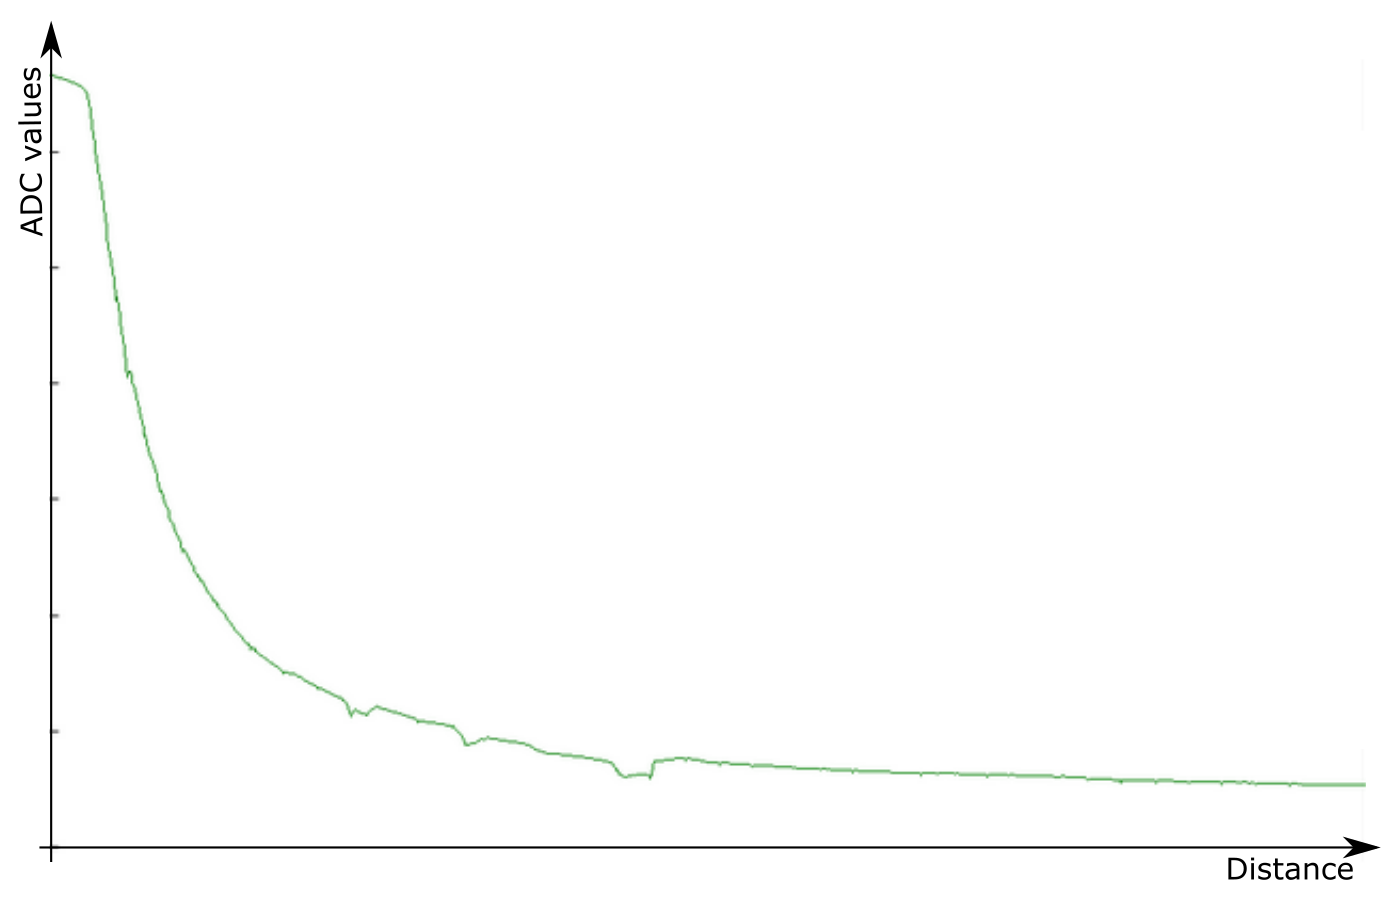
\includegraphics[width=0.8\textwidth]{figs/epuckirsensor.png}
	\caption{Typical response of an infrared distance sensor as a function of distance. Units are left dimensionless intentionally.}
	\label{fig:epuckir}
\end{figure}

Using more than one  sensor/emitter pair---e.g., using a pattern projector as emitter and a camera as receiver---not only allows to measure the distance of many points at once, but also to assess the structure of the environment by calculating its impact on the deformation of patterns. For example, a straight line becomes a curve when projected onto a round surface. This approach is known as \textsl{structured light}\index{Structured light} and is illustrated in Figure~\ref{fig:struclight}.
Thanks to the continuously increasing efficiency of computational systems, a light-weight version of such an approach has become feasible to be implemented at small scale and low cost around 2010, and emerged as a novel standard in robotic sensing.

\begin{figure}
	\centering
		\includegraphics[width=\textwidth]{figs/structuredlight.png}
	\caption{From left to right: two complex physical objects, a pattern of colored straight lines and their deformation when hitting the surfaces, reconstructed 3D shape. From \protect\cite{zhang2002rapid}.}
	\label{fig:struclight}
\end{figure}

Instead of using line patterns, infrared-based depth image sensors use a speckle pattern (a collection of randomly distributed dots with varying distances), and two computer vision concepts: \textsl{depth from focus} and \textsl{depth from stereo}.\index{Depth from Focus}\index{Depth from Stereo} When using a lens with a narrow focal depth, objects that are closer or farther away appear blurred (you can easily observe this on professional portrait photos, which often use this effect for aesthetic purposes under the name of ``bokeh'').
Measuring the ``blurriness'' of a scene (for known camera parameters) therefore allows an initial estimate of depth.
Conversely, depth from stereo works by measuring the disparity of the same object appearing in two images taken by cameras that are a known distance apart. Being able to identify the same object in both frames allows to calculate this disparity, and from there the distance of the object: the farther the object is, the smaller the disparity will be.
This is where the speckle pattern comes in handy: it simply requires to search for blobs with similar size that are close to each other.

\subsection{Phase shift}\label{sec:phaseshiftsensors}

As shown in Figure~\ref{fig:epuckir}, reflection can only be precise if distances are short. Instead of measuring the strength (aka amplitude) of the reflected signal, laser distance sensors measure the phase difference of the reflected wave. In order to do this, the emitted light is modulated with a wave-length that exceeds the maximum distance the scanner can measure.
If you were to use visible light and to do so at much slower speeds, you would see a light that keeps getting brighter, then getting darker, briefly turns off and then starts getting brighter again.
Thus, if you were to plot the amplitude of the emitted signal over time (i.e., its brightness), you would see a wave that crosses zero when the light is dark.
As light travels, this wave propagates through space with a constant distance (the wavelength) between its zero crossings. When it gets reflected, the same wave travels back (or at least parts of it that get scattered right back). For example, modern laser scanners\index{Laser range finder} emit signals with a frequency of 5 MHz (turning off 5 million times in one second). Together with the speed of light of approximately $300,000km/s$, this leads to a wavelength of $60m$ and makes such a laser scanner useful up to $30m$.

When the laser is now at a distance that corresponds exactly to one half the wave-length, the reflected signal it measures will be dark at the exact same time its emitted wave goes through a zero-crossing. Going closer to the obstacle results in an offset that can be measured. As the emitter knows the shape of the wave it emitted, it can calculate the phase difference between emitted and received signal. Knowing the wave-length it can now calculate the distance. As this process is mostly independent from ambient light, the estimates can be very precise.
% This is in contrast to a sensor that uses signal strength. As the signal strength decays at least quadratically, small errors, e.g.\ due to fluctuations in the power supply that drives the emitting light, noise in the analog-digital converter, or simply differences in the reflecting surface have drastic impact on the accuracy and precision (see below for a more formal definition of this term).

As the laser distance measurement process is fast, such lasers can be combined with rotating mirrors to sweep larger areas, known as \textsl{Laser Range Scanners}\index{Laser Range Scanners} or \textsl{Lidars}\index{Lidar}. Such systems have been combined into packages consisting of up to $64$ scanning lasers and are nowadays vastly used in the autonomous driving space as they are capable of providing a depth map around a car while driving.
It is also possible to modulate projected images with a phase-changing signal, which is the operational principle of early ``time-of-flight'' cameras, which however is not an accurate description of their operation.

\subsection{Time-of-flight}

The most precise distance measurements light can provide is by measuring its time of flight. This can be done by counting the time a signal from an emitter becomes visible in a receiver. As light travels very fast ($3\cdot10^8m/s$), this requires high-speed electronics that can measure time periods smaller than nanoseconds in order to achieve centimeter accuracy.
In practice, this is done by combining the receiver with a very fast electronic shutter that operates at the same frequency of the emitted light. As this timing is known, one can infer the time light has traveled by measuring the quantity of photons that made it back from the reflective surface within one shutter period.
As an example, light travels $15m$ in $50ns$. Therefore, it will take a pulse of $50ns$ to return from an object at a distance of $7.5m$. If the emitter transmits a pulse of $50ns$ length and then closes the receiver with a shutter, the receiver will receive more photons the closer the object is, but no photons if the object is farther than $7.5m$. Given a fast enough and precise circuit that acts as a shutter, it is sufficient to measure the actual amount of light that returns from the emitter.

\subsubsection{Ultra-sound distance sensors}
\label{sec:sensors:sound}

Measuring the time of flight is considerably simpler when using sound waves to measure distance (sound travels at around $344m/s$ in air). An ultra-sound distance sensor operates by emitting an ultra-sound pulse and measures its reflection. Unlike a light-based sensor that measures the amplitude of the reflected signal, a sound-based sensor measures the time it took for the pulse to travel back and forth.
This is possible because sound travels at much lower speed ($3\cdot10^2m/s$) than light ($3\cdot10^8m/s$). The fact that the sensor actually has to wait for the signal to return leads to a trade-off between range and bandwidth (see \cref{sec:sensors:terminology}: allowing a longer range requires waiting longer for the signal to come back, which in turn limits how often the sensor can provide a measurement.
% (Look these definitions up above before you read on.)\td{fix--up above where?}
Although ultrasound distance sensors have become progressively less common in robotics, they have an advantage over light-based sensors: instead of sending out a ray, the ultra-sound pulse results in a cone with an opening angle of $20$ to $40$ degrees. Because of this, such sensors are able to detect small obstacles without the requirement of directly hitting them with a ray. This property makes them the sensor of choice in specific applications, such as the automated parking assist technologies in modern cars.

\subsection{The relationship between distance and force}
As introduced in the context of series-elastic actuators, distance and force sensing are tightly related via Hooke's law. There exists a large variety of touch and force sensors that rely on light-based distance measurement in conjunction with a flexible material with known spring constant, such as using distance sensors to measure the deformation of an elastic dome from the inside \cite{youssefian2013contact} or measuring distance to objects through transparent rubber before touch and contact force after touch \cite{patel2018integrated}.


\section{Sensors to sense global pose}
So far, we have discussed sensors that allow the robot to measure the position of its own joints,  its rotational velocity, its translational acceleration, forces from interaction with the environment, and distance to objects relative to its own pose. In order to reliably navigate in the environment, robots also need some notion of a world coordinate frame.  

Localizing an object by triangulation goes back to ancient civilizations, where sailors oriented themselves using the stars. As stars are only visible during unclouded nights, seafarers have invented systems of artificial beacons emitting light, sound, and eventually radio waves. The most sophisticated of such systems is the Global Positioning System (GPS). GPS consists of a number of satellites in orbit that are equipped with knowledge about their precise location and have synchronized clocks. These satellites broadcast a radio signal that travels at the speed of light and is coded with its time of emission. GPS receivers can therefore calculate the distance to each satellite by comparing time of emission and time of arrival. As not only the position (x,y,z), but also the time difference between the GPS receiver's clock and the synchronized clocks of the satellites is unknown, four satellites are needed to obtain a ``fix''. Due to the way information from the satellites is coded, getting an initial fix can take in the order of minutes, but afterwards it becomes available multiple times per second. GPS measurements are neither precise nor accurate enough for robotics applications, and require to be combined with other sensors, such as IMUs and compasses. (Note that the bearing shown on some GPS receivers you may have access to is calculated from subsequent positions and is therefore meaningless if the robot is not moving.)

There exist also a variety of indoor GPS solutions, which consists of either active or passive beacons that are mounted in the environment at known locations. Passive beacons, for example infrared reflecting stickers arranged in a certain pattern or 2D barcodes, can be detected using cameras and their pose can be calculated from their known dimensions. Active beacons instead usually emit radio, ultrasound or a combination thereof, which can then be used to estimate the robot's range to this beacon.

\section*{Take-home lessons}
\begin{itemize}
\item Most of a robot's sensors either address the problem of determining the robot's pose or localizing and recognizing objects in its vicinity.
\item Each sensor has advantages and drawbacks that are quantified in its range, precision, accuracy, and bandwidth. Therefore, robust solutions to a problem can only be achieved by combining multiple sensors with differing operation principles.
\item Solid-state sensors (i.e.\ without mechanical parts) can be miniaturized and cheaply manufactured in quantity. This has enabled a series of affordable IMUs and 3D depth sensors that will provide the data basis for localization and object recognition on mass-market robotic systems.
\end{itemize}

\section*{Exercises}\small
\begin{enumerate}
\item Given a laser scanner with an angular resolution of 0.01 rad and a maximum range of 5.6 meters, what is the minimum range $d$ a robot needs to have from an object of 1cm width to definitely sense it, i.e., hit it with at least one of its rays? You can approximate the distance between two rays with the arc length.
\item Why does the bandwidth of a Ultra-sound based distance sensor decrease significantly when increasing its dynamic range, but that of a laser range scanner does not for typical operation?
\item You are designing an autonomous electric car to transport goods on campus. As you are worried about cost, you are thinking about whether to use a laser scanner or an ultra-sound sensor for detecting obstacles. As you drive rather slow, you are required to sense up to 15 meters. The laser scanner you are considering can sense up to this range and has a bandwidth of 10Hz. Assume 300m/s for the speed of sound in the following.
\begin{enumerate}
\item Calculate the time it takes until you hear back from the US sensor when detecting an obstacle 15m away. Assume that the robot is not moving at this point.
\item Calculate the time it takes until you hear back from the laser scanner. Hint: you don’t need the speed of light for this, the answer is in the specs above.
\item Assume now that you are moving toward the obstacle. Which sensor will give you a measurement that is closer to your real distance at the time of reading and why?
\end{enumerate}
\item Pick an educational robot platform of your choice and make a list of its sensors.
\item Construct a simple range scanner by mounting an ultra-sound sensor onto a servo motor. Implement a scanning routine that allows you to collect the raw data and display it on the screen. Can you see simple features such as corners and openings?
\item Explore the internet for do-it-yourself robotics shops. What kind of sensors do they offer? What are the interfaces these sensors provide?
\item Pick a physical sensor that you have access to. Can you design an experiment to characterize its precision and accuracy?
\item Your task is to design a sensor that can detect the remaining void in a parcel for an e-commerce application.
\begin{enumerate}
\item What sensors could you think off that would allow you to measure the volume of the content in the box?
\item What additional sensors could you use assuming the box is moving on a conveyor belt.
\item What additional information would you need to know in order to differentiate between box content, the box itself, and the environment around the box? What sensors could you use to get this information?
\item Additional sensors are not within your budget. What kind of measures could you take to reduce the amount of information required?
\end{enumerate}
\item Your task is to design an autonomous cart that can automatically dock with shelves in the environment.
\begin{enumerate}
\item What kind of sensors could you use to locate the shelf in the environment? Assume that the shelf is the only object in a certain target area.
\item What kind of physical measures could you take to simplify detection of the shelf?
\item  What kind of sensors could you use to detect whether the shelf is in a suitable position for docking?
\item What kind of physical measures could you take to simplify the sensing process?
\end{enumerate}
\item You are designing a competitive controller for the ``Ratslife'' game. What kind of information does the environment provide and what kind of sensor would you need to exploit it?
\end{enumerate}\normalsize


\part{Computation}
\chapter{Vision}\label{chap:vision}
Vision is one of the information-rich sensor system both humans and robots have available. Processing the wealth of information that is generated by vision sensors is still a key challenge, however. The goal of this chapter is to introduce
\begin{itemize}
\item images as two-dimensional signals,
\item provide an intuition of the wealth of information hidden in low-level information,
\item introduce basic convolution and threshold-based image processing algorithms.
\end{itemize}

\section{Images as two-dimensional signals}
Images are captured by cameras containing matrices of charge-coupled devices (CCD) or similar semi-conductors that can turn photons into electrical signals. These matrices can be read out pixel by pixel and turned into digital values, for example an array of 640 by 480 three-byte tuples corresponding to the red, green, and blue (RGB) components the camera has seen. An example of such data, for simplicity only one color channel, is shown in Figure~\ref{fig:iss_closeup}.

Looking at the data clearly reveals the white tile within the black tiles at the lower-right corner of the chessboard. Higher values correspond to brighter colors (white) and lower values to darker colors. We also observe that although the tiles have to have the same color, the actual values differ quite a bit. It might make sense to think about these values much like we would do if the data would be 1D signal: taking the ``derivative'', e.g., along the horizontal rows, would indicate areas of big changes, whereas the ``frequency'' of an image  would indicate how quickly values change. Areas with smooth gradients, e.g., black and white tiles, would then have low frequencies, whereas areas with strong gradients, would contain high frequency information.

\begin{figure}[!htb]
	\centering
		\includegraphics[width=\textwidth]{figs/iss_closeupmatrix}
	\caption{A chessboard floating inside the ISS, astronaut Gregory Chamitoff. The inset shows a sample of the actual data recorded by the image sensor. One can clearly recognize the contours of the white tile.}
	\label{fig:iss_closeup}
\end{figure}

This language opens the door to a series of signal processing concepts, such as low-pass filters (supressing high frequency information), high-pass filters (suppressing low frequency information), or band-pass filters (letting only a range of frequencies pass), analysis of the frequency spectrum of the image (the distribution of content at different frequencies), or ``convolving'' the image with another two-dimensional function. The next sections will provide both an intuition of what kind of meaningful information is hidden in such abstract data and provide concrete examples of signal processing techniques that make this information appear.

\section{From signals to information}
Unfortunately, many phenomena that often have very different or even opposite meaning look very similar when looking at the low-level signal. For example, drastic changes in color values do not necessarily mean that the color of a surface indeed has changed. Similar patterns are generated by depth discontinuities, specular highlights, changing lighting conditions, or surface orientation changes. These examples are illustrated in Figure~\ref{fig:iss_edges} and make computer vision a hard problem.

\begin{figure}[!htb]
	\centering
		\includegraphics[width=\textwidth]{figs/iss_edges}
	\caption{Inside of the international space station (left), highlighted areas in which pixel values change drastically (right). Underlying effects that produce similar responses: change in surface properties (1), depth discontinuities (2), specular highlights (3), changing lighting conditions such as shadows (4), or surface orientation changes (5).
	\label{fig:iss_edges}}
\end{figure}

This example illustrates that signals alone are not sufficient to understand a phenomenon, but require context. Here, the context does not only refer to surrounding signals, but also high-level conceptional knowledge such as the fact that light sources create shadows and specular highlights, that objects in the front appear larger, and so on. How important such conceptional knowledge is, is illustrated by Figure~\ref{fig:craters}.

Both images show an identical landscape that once appears to be speckled with craters, once with bubble-like hills. At first glance, both scenes are illuminated from the left, suggesting a change in the landscape. Once information that the sun is illuminating one picture from the left and the other from the right, however, it becomes clear that the craters are simply differently illuminated and what we perceive as bumps eventually turns back into craters.

\begin{figure}[!htb]
	\centering
		\includegraphics[width=\textwidth]{figs/craters}
	\caption{Picture of the Apollo 15 landing site during different times of the day. The landscape is identical, but appears to be speckled with craters (lift) or hills (right). Knowing that the sun is illuminating the scene from the left and right, respectively, does explain this effect. Image credit: NASA/GSFC/Arizona State University.
	\label{fig:craters}}
\end{figure}

More surprisingly, conceptual knowledge is often sufficient to make up for the lack of low-level cues in an image. An example is shown in Figure~\ref{fig:dalmatian}. Here, a Dalmatian dog can be clearly recognized despite absence of cues for its outline, simply by extrapolating its appearance and pose from conceptual knowledge.

These examples illustrate both the advantages and drawbacks of a signal processing approach. While an algorithm will detect interesting signals even there where we don't see, or don't expect them (due to conceptional bias), image understanding not only requires low-level processing, but intelligent combination of the low-level cue's spatial relationship and conceptual knowledge about the world.


\begin{figure}
	\centering
		\includegraphics[width=\textwidth]{figs/dalmatian}
	\caption{The image of a Dalmatian dog can be clearly recognized by most spectators even though low-level cues such as edges are only present for ears, chin and parts of the legs. The contours of the animals are highlighted in a flipped version of the image in the inset.
	\label{fig:dalmatian}}
\end{figure}

\section{Basic image operations}
Basic image operations can be thought of as a filter that operates in the frequency or in the space (color) domain. Although most filters directly operate in the color domain, knowing how they affect the frequency domain is helpful in understanding the filter's function. For example, a filter that is supposed to highlight edges, such as shown in Figure~\ref{fig:iss_edges} should suppress low frequencies, i.e., areas in which the color values do not change much, and amplify high-frequency information, i.e., areas in which the color values change quickly. The goal of this section is to provide a basic understanding of how basic image processing operation works. The methods presented here, while still valid, have been superseded by more sophisticated implementations that are widely available as software packages or within desktop graphic software.

\subsection{Convolution-based filters}
 A filter can be implemented using the \emph{convolution}\index{Convolution} operator that convolves function $f()$ with function $g()$.
\begin{equation}
f(x)\star g(x)=\int_{-\infty}^{\infty}f(\tau)g(x-\tau)d\tau
\end{equation}
We then call function $g()$ a \emph{filter}\index{Filter}. As will become more clear further below, the convolution literally shifts the function $g()$ across the function $f()$ while multiplying the two. As images are discrete signals, the convolution is usually discrete
\begin{equation}
f[x]\star g[x]=\sum_{i=-\infty}^{\infty}f[i]g[x-i]
\end{equation}
For 2D signals, like images, the convolution is also two-dimensional:
\begin{equation}\label{eq:2dconv1}
f[x,y]\star g[x,y]=\sum_{i=-\infty}^{\infty}\sum_{j=-\infty}^{\infty}f[i,j]g[x-i,y-j]
\end{equation}
Although we have defined the convolution from negative infinity to infinity, both images and filters are usually finite. Images are constrained by their resolution, and filters are usually much smaller than the images themselves. Also, the convolution is commutative, therefore (\ref{eq:2dconv1}) is equivalent to
\begin{equation}\label{eq:2dconv2}
f[x,y]\star g[x,y]=\sum_{i=-\infty}^{\infty}\sum_{j=-\infty}^{\infty}f[x-i,y-j]g[i,j].
\end{equation}

\subsubsection{Gaussian smoothing}
A very important filter is the Gaussian filter.\index{Gaussian filter} It is shaped like the Gaussian bell function and can be easily stored in a 2D matrix. Implementing a Gaussian filter is surprisingly simple, e.g., such as
\begin{equation}
g(x,y)=\frac{1}{10}
\left(
\begin{array}{ccc}
1 & 1 & 1\\
1 & 2 & 1\\
1 & 1 & 1\\
\end{array}
\right)
\end{equation}
Using this filter in Equation~\ref{eq:2dconv2} on an infinitely large image $f()$ leads to
\begin{equation}\label{eq:2dconv3}
f[x,y]\star g[x,y]=\sum_{i=-1}^{1}\sum_{j=-1}^{1}f[x-i,y-j]g[i,j]
\end{equation}
(assuming $g(0,0)$ addresses the center of the matrix). What now happens is that each pixel $f(x,y)$ becomes the average of that of its neighbors, with its previous value weighted twice (as $g(0,0)=0.2$) that of their neighbors. More concretely,
\begin{equation}
f(x,y)=
\begin{smallmatrix*}[lll]
f(x+1,y+1)g(-1,-1) &+f(x+1,y)g(-1,0) &+f(x+1,y-1)g(-1,1)\\
+f(x,y+1)g(0,-1) &+f(x,y)g(0,0) &+f(x,y-1)g(0,1)\\
+f(x-1,y+1)g(1,-1) &+f(x-1,y)g(1,0) &+f(x-1,y-1)g(1,1)
\end{smallmatrix*}
\end{equation}
Doing this for all $x$ and all $y$ literally corresponds to sliding the filter $g()$ along the image.

\begin{figure}
	\centering
		\includegraphics[width=\textwidth]{figs/filters}
	\caption{A noisy image before (top left) and after filtering with a Gaussian kernel (top right). Corresponding edge images are shown underneath.
	\label{fig:filters}}
\end{figure}

An example of filter $g(x,y)$ in action is shown in Figure~\ref{fig:filters}. The filter acts as a \emph{low-pass filter}\index{Low-pass filter}, suppressing high frequency components. Indeed, noise in the image is suppressed, leading also to a smoother edge image, which is shown underneath.

\subsubsection{Edge detection}\label{sec:sobel}
Edge detection can be achieved using another convolution-based filter, the \emph{Sobel} kernel\index{Sobel filter}
\begin{equation}
s_x(x,y)=
\left(
\begin{array}{ccc}
-1 & 0 & 1\\
-2 & 0 & 2\\
-1 & 0 & 1\\
\end{array}
\right)
\qquad
s_y(x,y)=
\left(
\begin{array}{ccc}
1 & 2 & 1\\
0 & 0 & 0\\
-1 & -2 & -1\\
\end{array}
\right)
\end{equation}
Here, $s_x(x,y)$ can be used to detect vertical edges, whereas $s_y(x,y)$ highlights horizontal edges. Edge detectors, such as the \emph{Canny} edge detector\index{Canny edge detector}  therefore run at least two of such filters over an image to detect both horizontal and vertical edges.

\subsubsection{Difference of Gaussians}
An alternative method for detecting edges is the \emph{Difference of Gaussians} (DoG) method\index{Difference of Gaussians (DoG)}. The idea is to subtract two images that have each been filtered using a Gaussian kernel with different width. Both filters supress high-frequency information and their difference therefore leads to a \emph{band-pass} filtered signal\index{Band-pass filter}, from which both low and high frequencies have been removed. As such, a DoG filter acts as a capable edge detection algorithm. Here, one kernel is usually four to five times wider than the other, therefore acting as a much stronger filter.

Differences of Gaussians can also be used to approximate the \emph{Laplacian of Gaussian}\index{Laplacian of Gaussian}, i.e., the sum of the second derivatives of a Gaussian kernel. Here, one kernel is roughly 1.6 times wider than the other. The band-pass characteristic of DoG and LoGs are important as they highlight high-frequency information such as edges, yet suppress high-frequency noise in the image.


\subsection{Threshold-based operations}
In order to find objects with a certain color or edge intensity, thresholding an image will lead to a binary image that contains ``true-false'' regions that fit the desired criteria. Thresholds make use of operators like $>,<,\leq,\geq$ and combinations thereof. There also exist adaptive versions that would adapt the thresholds locally, e.g., to make up for changing lighting conditions.

Albeit thresholding is deceptively simple, finding correct threshold values is a hard problem. In particular, actual pixel values change drastically with changing lighting conditions and there is no such thing as ``red'' or ``green'' when inspecting the actual values under different conditions.

\subsection{Morphological Operations}
Another class of filters are morphological operators which consists of a kernel describing the structure of the operation (this can be as simple as an identity matrix) and a rule on how to change a pixel value based on the values in the neighborhood defined by the kernel.

Important morphological operators are \emph{erosion} and \emph{dilation}\index{Erosion}\index{Dilation}. The erosion operator assigns a pixel value with the minimum value that it can find in the neighborhood defined by the kernel. The dilation operator assigns a pixel value with the maximum value it can find in the neighborhood defined by the kernel. This is useful, e.g., to fill holes in a line or remove noise. A dilation followed by an erosion is known as a ``Closing'' and an erosion followed by a dilation as an ``Opening''. Subtracting erosed and dilated images from each other can also serve as an edge detector. Examples of such operators are shown in Figure~\ref{fig:morphology}.

\begin{figure}
	\centering
		\includegraphics[width=\textwidth]{figs/morphology}
	\caption{Examples of morphological operators erosion and dilation and combinations thereof.
	\label{fig:morphology}}
\end{figure}


\section*{Exercises}\small
\begin{enumerate}
\item Below are shown multiple ``Kernels'' that can be used for convolution-based image filtering.
\begin{equation}
\nonumber
\begin{array}{|c|c|c|}
\hline
1 & 1 & 1\\
\hline
1 & 2 & 1\\
\hline
1 & 1 & 1\\
\hline
\end{array}
\quad
\begin{array}{|c|c|c|}
\hline
0 & -1 & 0\\
\hline
0 & -1 & 0\\
\hline
0 & -1 & 0\\
\hline
\end{array}
\quad
\begin{array}{|c|c|c|}
\hline
1 & 1 & 1\\
\hline
1 & -4 & 1\\
\hline
1 & 1 & 1\\
\hline
\end{array}
\end{equation}
\begin{enumerate}
\item Identify the Kernel, which can blur an image.
\item What kind of features can be detected by the other two kernels?
\end{enumerate}
\item How many for-loops are needed to implement a 2D convolution? Explain your reasoning.
\end{enumerate} \normalsize

\chapter{Feature extraction}\label{chap:feature_extraction}

A robot can obtain information about its environment by both active (e.g., ultrasound, light, and laser) or passive sensing (e.g., acceleration, magnetic field, or cameras). There exist only limited cases where this information is directly useful to a robot and does not require significant preprocessing over it. For example, before being able to arrive at semantic information such as ``I'm in the kitchen'', ``this is a cup'' or ``this is a horse'', one must first identify higher-level \textsl{features}\index{Features} and correlate these features with the information of interest.

The goal of this chapter is to introduce the notion of features, and understand standard feature detectors such as:

\begin{itemize}
    \item the Hough-transform to detect lines, circles and other shapes,
    \item numerical methods such as least-squares, split-and-merge and RANSAC to find high-level features in noisy data,
    \item scale-invariant features (SIFT).
\end{itemize}

\section{Feature detection as an information-reduction problem}
The information generated by sensors can be quite voluminous. For example, a simple webcam generates 640$\times$480 color pixels (red, green and blue) or 921600 bytes around 30 times per second. A single-ray laser scanner provides around 600 distance measurements 10 times per second in the form of a point cloud. Consider for a moment the information that a robot \emph{requires} in order to solve its problems, however. The volume of data resulting from most sensors seems much greater than the amount of information required to answer the query ``what are the dimensions of this room?'' Consider for example the maze-solving competition ``Ratslife'' (\cref{sec:ratslife}) in which the robot's camera can be used to recognize one of 48 different color patterns (\cref{fig:ratslife}) that are distributed in the environment, or the presence or absence of a charger, essentially reducing hundreds of bytes of camera data to 6 bits of content ($2^6=64$ different values). The goal of most image processing algorithms is therefore to first reduce information content in a meaningful way and then extract relevant information. In Chapter~\ref{chap:vision}, we were introduced to convolution-based filters such as blurring, detecting edges, or binary operations such as thresholding. We are now interested in methods to extract higher-level features such as lines and techniques to extract them using these types of processing algorithms.

\section{Features}
Lines are particularly useful features for localization and can correspond to walls in 2D laser scans, edges in 3D laser scans, markers on the floor, or corners detected in a camera image. Whereas a Sobel filter (\cref{sec:sobel}) can help us to highlight lines and edges in images, additional algorithms are needed to identify the line and extract structured information such as it's position and orientation. This structured information can then aid in identifying these lines and edges through multiple observations, which admits reasoning over persistent structures and our motion against them.

A desirable property of a feature is that its extraction is repeatable and robust to rotation, scale, and noise in the data. We need feature detectors that can extract the same feature from sensor data, even if the robot has slightly turned or moved farther or closer to the feature. Ideally the same feature could also be extracted if there is some noise affecting the sensor. There are many feature detectors available that accomplish this. Prominent examples are the \emph{Harris corner detector}\index{Harris Corner Detector}, which detects points in the image where vertical and horizontal lines cross, and the scale-invariant feature transform (SIFT) detector\index{SIFT features}, which identifies features through maxima in the difference-of-Gaussian image (\cref{sec:vision:dog}) at various spatial scales. Feature detection is important far beyond robotics and is for example used in hand-held cameras that can automatically stitch images together and image indexing on the Internet. In image stitching, feature detectors will ``fire'' (identify a feature) on the same features in two images taken from slightly different perspectives; these matched features provide a geometric template between the images where information is shared, thereby allowing for the two images to be concatenated.

This chapter focuses on two important classes of features: line features and scale-invariant features in images (SIFT). Both classes of features provide tangible examples for the least-squares and RANSAC algorithms, which may be used to harness feature information to solve problems, and are also introduced in this chapter. Together, these classes of features are fairly representative of all features used in robotics, and have been chosen for their simplicity, providing a basis for understanding the function of more complex feature detectors.

These hand-coded feature detectors are in contrast to entirely self-learned feature detectors based on deep neural networks, which are treated in Chapter \cref{chap:ann}. Although neural network-based methods often outperform hand-coded features, hand-coded features remain relevant for environments in which learning is unfeasible, to preprocess data before subjecting it to a learning-based method, or to understand what kind of architecture is required to solve a specific goal.

\section{Line recognition}
\label{sec:line_recognition}
Why are lines a useful feature? As you will see in the ``uncertainty'' part of the book, the key challenge in estimating a robot's pose is unreliable odometry, in particular when it comes to turning. Here, a simple infrared sensor measuring the distance to a wall can provide the robot with a much better sense for what actually happened during the turn. Similarly, if a robot has the ability to track markers in the environment using vision, it gets another measurement on how much the robot is actually moving. How information from odometry and other sensors can be fused not only to localize the robot, but also to create maps of its environment, will be a significant focus in the remainder of this book.

A laser scanner or similar device pointed at a wall will return a measurement of $N$ points at position $(x_i,y_i)$ in the robot's coordinate system. These points can also be represented in polar coordinates $ (\rho_i,\theta_i)$. We can now imagine a line running through these points that is parametrized with a distance $r$ and an angle $\alpha$. Here, $r$ is the distance of the robot to the wall and $ \alpha$ its angle. As all sensors are noisy, each point will have distance $d_i$ from the ``optimal'' line running through the points. These relationships are illustrated in \cref{fig:linefitting}.

\begin{figure}
	\centering
	% 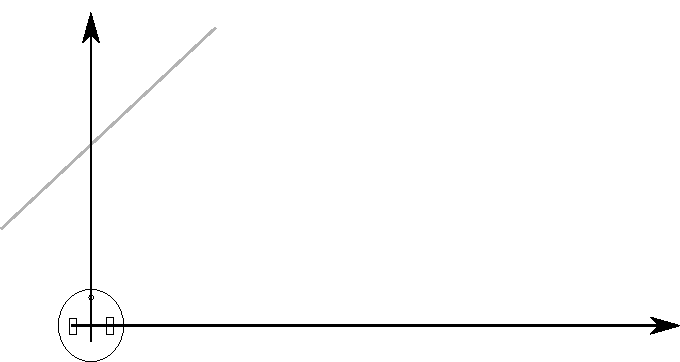
\includegraphics[width=\textwidth]{figs/linefitting.png}
    \def\svgwidth{\textwidth}
    \import{./figs/}{linefitting.pdf_tex}
	\caption{A 2D point cloud recorded by a laser scanner or similar device. A line (dashed) is fitted through the points in a least-square sense.}
	\label{fig:linefitting}
\end{figure}

\subsection{Line fitting using least squares}
Using simple trigonometry we can now write:
\begin{equation}
\rho_i \cos(\theta_i-\alpha)-r=d_i.
\end{equation}

Different line candidates---parametrized by $ r$ and $ \alpha$---will have different values for $ d_i$. We can now write an expression for the total error $ S_{r,\alpha}$ as:

\begin{equation}
S_{r,\alpha}=\sum_{i=1}^{N}{d_i^2}=\sum_i(\rho_i \cos(\theta_i-\alpha)-r)^2.
\end{equation}

Here, we square each individual error to account for the fact that a negative error, i.e.\ a point left of the line, is as bad as a positive error, i.e.\ a point right of the optimal line. In order to optimize $ S_{r,\alpha}$, we need to take the partial derivatives with respect to $ r$ and $ \alpha$ and set them zero, indicating the functions are at their minimum or maximum:

\begin{equation}
\frac{\partial{S}}{\partial{\alpha}}=0 \qquad \frac{\partial{S}}{\partial{r}}=0,
\label{eq:partialzeros}
\end{equation}

\noindent and then solve the resulting system of Equations \eqref{eq:partialzeros} for $ r$ and $ \alpha$. Here, the symbol $ \partial$ indicates that we are taking a partial derivative. Solving for $r$ and $\alpha$ is algebraically, but possible \cite{siegwart2011introduction}:

\begin{equation}\label{eq:linealpha}
\alpha=\frac{1}{2}\text{atan}\left(\frac{\frac{1}{N}\sum{\rho_i^2 \sin 2\theta_i}-\frac{2}{N^2}\sum{\sum{\rho_i\rho_j \cos \theta_i \sin \theta_j}}}{\frac{1}{N}\sum{\rho_i^2 \cos 2 \theta_i - \frac{1}{N^2}\sum{\sum{\rho_i \rho_j \cos(\theta_i+\theta_j)}}}}\right),
\end{equation}

\noindent and

\begin{equation}\label{eq:liner}
r=\frac{{\sum \rho_i \cos (\theta_i-\alpha)}}{N}.
\end{equation}

Therefore, using our proximity sensors, we can calculate the distance and orientation of a wall relative to the robot's positions, or the height and orientation of a line in an image, based on a collection of points that we believe might belong to a line.

This approach is known as the \textsl{least-squares method}\index{Least-Squares Method (Line fitting)} and can be used to fit data to any parametric model (i.e.\ a model that has numbers to be sought to make it fit our data best). The general approach is to describe the fit between the data and the model in terms of a difference, known as an ``error''. The best fit will minimize this error, i.e.\ the error will have a zero derivative for the best parameters. If the result cannot be obtained analytically as in this example, numerical methods have to be used to find the best fit that minimizes the error.

\subsection{Split-and-merge algorithm}
It is often unclear how many lines there are and where a line starts and ends. This creates a challenge for the matching-and-estimation strategy discussed above. Looking through the camera, for example, we will see vertical lines corresponding to wall corners and horizontal ones that correspond to wall-floor intersections and the horizon; using a distance sensor, the robot might detect a corner. We therefore need an algorithm that can separate point clouds into multiple lines. One possible approach is to find the outlier with the strongest deviation from a fitted line and split the line at this point. This is illustrated in \cref{fig:splitandmerge}. This can be done iteratively until each line has no outliers above a certain threshold.

\begin{figure}
    % 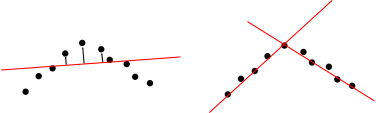
\includegraphics[width=\textwidth]{figs/splitandmerge}
    \def\svgwidth{\textwidth}
    \import{./figs/}{splitandmerge.pdf_tex}
    \caption{Split-and-merge algorithm. Initial least-square fit of a line (left). Splitting the data-set at the point with the highest error (after picking a direction) allows fitting two lines with overall lesser error.\label{fig:splitandmerge}}
\end{figure}

\subsection{RANSAC: Random Sample and Consensus}
\screencast{https://youtu.be/9D5rrtCC_E0}{RANSAC}
If the number of outliers is large, a least squares fit will generate poor results as it will generate the ``best'' fit that accomodates both inliers and outliers. Note that this generally results in a very poor fit, since the least squares fit mathematically assigns a significant weight to outliers---not treating them as a single measurement to be discarded, but a cumulative error to be reduced in balance with those of the inliers. In this way, split-and-merge algorithms will fail as they are extremely sensitive to outliers: depending on the actual parameters every outlier will split a potential line into two.

A powerful solution to this problem is to randomly sample possible lines and keep those that satisfy a certain desired quality given by the number of points being somewhat close to the best fit. This is illustrated in \cref{fig:ransac}, with darker lines corresponding to better fits. RANSAC\index{RANSAC}\index{Random Sample and Consensus} usually requires two parameters, namely the number of points required to consider a line to be a valid fit, and the maximum $d_i$ from a line to consider a point an inlier and not an outlier. The algorithm proceeds as follows: select two random points from the set and connect them with a line. Grow this line by $d_i$ in both directions and count the number of inliers. Repeat this until one or more lines that have sufficient number of inliers are found, or a maximum number of iterations is reached. RANSAC is applied frequently when it comes to feature detection and matching as it provides a systematic routine for separating inliers from outliers in even very noisy data.

\begin{figure}
    \center
    % 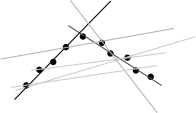
\includegraphics[width=0.6\textwidth]{figs/ransac}
    \def\svgwidth{0.6\textwidth}
    \import{./figs/}{ransac.pdf_tex}
    \caption{Random Sample and Consensus (RANSAC). Random lines are evaluated by counting the number of points close by (``inliers''), darker lines are better fits.\label{fig:ransac}}
\end{figure}

The RANSAC algorithm is fairly easy to understand in the line fitting application, but can be used to fit arbitrary parametric models to any-dimensional data. Here, its main strength is to cope with noisy data.

Given that RANSAC is random, finding a really good fit can be computationally intensive and time-consuming. Therefore, RANSAC is usually used only as a first step to get an initial estimate, which can then be improved by some kind of local optimization, such as least-squares.

\subsection{The Hough transform}
The Hough transform \index{Hough transform} can best be understood as a voting scheme to guess the parametrization of a feature such as a line, circle or other curve \cite{duda1972use}. For example, a line might be represented by $y=mx+c$, where $m$ and $c$ are the gradient and offset. A point in this parameter space (or ``Hough-space'') then corresponds to a specific line in $x$-$y$-space (or ``image-space''). The Hough transform now proceeds as follows: for every pixel in the image that could be part of a line, e.g., white pixels in a thresholded image after Sobel filtering, construct all possible lines that intersect this point. (Drawing an image of this would look like a star). Each of these lines has a specifc $m$ and $c$ associated with it, for which we can add a white dot in Hough-space. Continuing to do this for every pixel of a line in an image will yield many $m-c$ pairs, but only one that is common among all those pixels of the line in the image: the actual $m-c$ parameters of this line. Thinking about the number of times a point was highlighted in Hough-space as brightness, will turn a line in image space into a bright spot in Hough-space (and the other way around). In practice, a polar representation is chosen for lines, as shown in \cref{fig:hough}. The Hough transform also generalizes to other parametrization such as circles.

\begin{figure}
    \center
    % 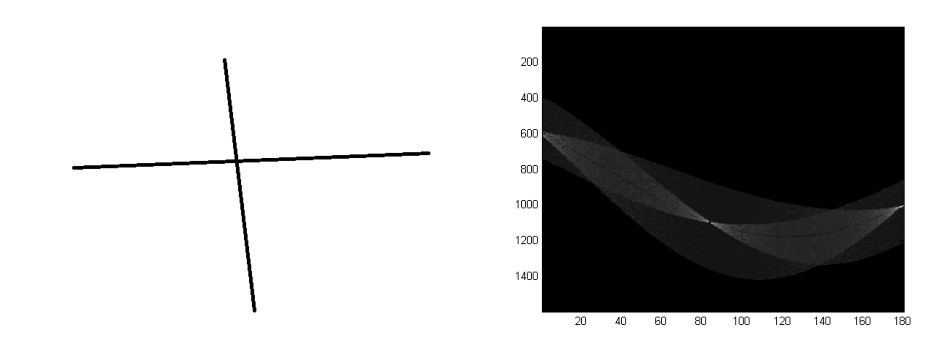
\includegraphics[width=\textwidth]{figs/houghtransform}
    \def\svgwidth{\textwidth}
    \import{./figs/}{houghtransform.pdf_tex}
    \caption{Lines in an image (left) transposed into Hough-space $\rho$ (distance from origin) and $\theta$ (angle of normal with respect to origin). Bright spots in the Hough image (right) correspond to parameters that have received the most ``votes'' and clearly show the two lines at around 90$^\circ$ and 180$^\circ$.\label{fig:hough}}
\end{figure}


\section{Scale-invariant feature transforms}
Scale-invariant feature transforms (SIFT) are a class of algorithms that allow to extract features that are easily detectable across different scales (or distances to an object), independent of their rotation, and to some extent robust to perspective transformations and illumination changes. An early algorithm in this class is the SIFT algorithm \cite{lowe1999object},\index{SIFT} which has lost some popularity due to its licensing, and has been replaced in the past with SURF (Speeded-Up Robust Feature) \cite{bay2006surf}\index{SURF} and ORB \cite{rublee2011orb}, which are freely available. As the arithmetic behind SURF is slightly more involved, we focus on the intuition behind SIFT and encourage the reader to download and play with the various open-source implementations of other feature detectors that are freely available.



\subsection{Overview}
SIFT proceeds in multiple steps. Descriptions of the algorithm often include its application to object recognition, but these algorithms are independent of the feature generation step.

\begin{enumerate}
\item Differences of Gaussians (DoG) at different scales:
\begin{enumerate}
\item Generate multiple scaled versions of the same image by re-sampling every 2nd, 4th, and so on (up to the desired scale), pixel.
\item Filter each scaled picture with various Gaussian filters of different variance.
\item Calculate the difference between pairs of filtered images. This is equivalent to a DoG filter.
\end{enumerate}

\item Detecting local minima and maxima in the DoG images across different scales (\cref{fig:siftrejection}, left) and reject those with low contrast (\cref{fig:siftrejection}, right).

\begin{figure}
	\centering
	\includegraphics[width=\textwidth]{figs/siftrejection.png}
	\caption{After scale space extrema are detected (left), the SIFT algorithm discards low contrast keypoints (center) and then filters out those located on edges (right). \copyright Lukas Mach CC-BY 3.0}
	\label{fig:siftrejection}
\end{figure}

\item Reject extrema that are along edges by looking at the second partial derivatives in image space around each extremum (\cref{fig:siftrejection}, right). Edges have a much larger principal curvature across them than along them.
\item Assign a ``magnitude'' and ``orientation'' to each remaining extremum, now called a ``keypoint''. The magnitude is the squared difference between the DoG filter response at the present pixel and the neighboring pixels. The orientation is the arctangent between the DoG differences in the $y$ direction and the $x$ direction. These calculations are made for all pixels in a fixed neighborhood around the initial keypoint, e.g., in a 16$\times$16 pixel neighborhood.
\item Collect orientations of neighboring pixels in a histogram, e.g., 36 bins each covering 10 degrees. Maintain the orientation corresponding to the strongest peak and associate it with the keypoint.
\item Repeat step 4, but for four $4\times4$ pixel areas around the keypoint in the image scale that has the most extreme minima/maxima. Here, only 8 bins are used for the orientation histogram. As there are 16 histograms in a 16$\times$16 pixel area, the feature descriptor has 128 dimensions.
\item The feature descriptor vector is normalized, tresholded, and again normalized to make it more robust against illumination changes.
\item Local gradient magnitude and orientation are grouped into bins and create a 128-dimensional feature descriptor.
\end{enumerate}

The resulting 128 dimensional feature vectors are now scale-invariant (due to step 2), rotation-invariant (due to step 5), and robust to illumination changes (due to step 7).

\subsection{Object Recognition using scale-invariant features}
Scale-invariant features of training images can be stored in a database and can be used to identify these objects in the future. One approach to this is to find all features in an image and comparing them with those in the database. This comparison is done by using the Euclidian distance as metric and searching a $k$-$d$ tree (with $d=128$). In order to make this approach robust, each object needs to be identified by at least 3 independent features. For this, each descriptor stores the location, scale and orientation of it relative to some common point on the object. This allows each detected feature to ``vote'' for the position of the object that it is most closely associated with in the database.  This is done using a Hough-transform. For example, position (2 dimensions) and orientation (1 dimension) can be discretized into bins (30 degree width for orientation); bright spots in Hough-space then correspond to an object pose that has been identified by multiple features. Another popular approach uses the Bag of Words (BoW) technique, in which features are collected into groups that compose a ``word.'' The words are then matched against query features to determine the similarity between the collected features and the query features, and thus a measure of likelihood that the object in the image is that of the query.

\section{Feature detection and machine learning}
This chapter has introduced a variety of algorithms that turn high-dimensional input data into low-dimensional features, which can then be used to further reason about a problem. Recent advances in artificial neural networks (Chapter \ref{chap:ann}) have not only allowed us to automatically train such feature detectors from data, but also often outperform hand-coded feature detectors such as SIFT. Whereas the last decades have been dominated by hand-coding image understanding pipelines consisting of filtering, feature detection and thresholding (see also Chapter \ref{chap:vision}), modern neural network-based pipelines perform all these steps in the different layers of their network architecture. Like with low-level pre-processing (Chapter \ref{chap:vision}), understanding basic feature detection algorithms remains important to understand what the different components of a neural network actually do as well as how to deal with data for which no training information are available. 

\section*{Take-home lessons}
\begin{enumerate}
\item Features are ``interesting'' information in sensor data that are robust to variations in rotation and scale as well as noise.
\item Which features are most useful depends on the characteristics of the sensor generating the data, the structure of the environment, and the actual application.
\item There are many feature detectors available some of which operating as simple filters, others relying on machine learning techniques.
\item Lines are among the most important features in mobile robotics as they are easy to extract from many different sensors and provide strong clues for localization.
\end{enumerate}

\section*{Exercises}\small
\begin{enumerate}
\item Think about what information would make good features in different operating scenarios: a supermarket, a warehouse, a cave.
\item What other features could you detect using a Hough transform? Can you find parameterizations for a circle, a square or a triangle?
\item Do an online search for SIFT. What other similar feature detectors can you find? Which provide source code that you can use online?
\item A line can be represented by the function $y=mx+c$. Then, the Hough-space is given by a 2D coordinate system spanned by $m$ and $c$.\begin{enumerate}
\item Think about a line representation in polar coordinates. What components does the Hough-space consist of in this case?
\item Derive a parameterization for a circle and describe the resulting Hough space.
\end{enumerate}
\item Implement a detector for the various targets in Ratslife. Start with basic 2D images, then think about what you need to change in order to find targets in any possible orientation.
\item Simulate, build or get access to a range finder. Can you write an algorithm that reliably detects corners and openings?
\end{enumerate}
\normalsize

\chapter{Artificial Neural Networks}
Artificial neural networks are a specific flavor of machine learning that are loosely inspired by neural operation in the human brain and are able to classify or regress data, or to serve as a controller.

While artificial neural networks have long time been one out of many go-to methods from the vast field of machine learning to address these problems, recent advances in computing, in particular graphical processing units (GPU) and the availability of large datasets, which in turn resulted into the ability to train very, very large neural networks, also known as ``deep learning'', that have led to revolutionary results in many fields including computer vision, natural language processing, video and speech processing, and robotics.

Not too long ago, neural networks have been considered ``deep'' with more than two layers. Today, ``deep'' neural networks can have hundreds of layers and thousands of inputs and output, or more. This is still shy of the human brain, or even tiny areas thereof, which contains 100 billion neurons, each with thousands of synapses connecting a single neuron to thousands of others.

\section{When to use machine learning?}
Machine learning is a large field that shares many of the foundations in probability theory and statistics with robotics. The goal of this chapter is to provide a basic understanding of simple and recurrent neural networks that is sufficient to connect these tools to other topics in this book. In particular, deep learning can be used as a drop-in replacement for forward and inverse kinematics, sensor preprocessing and conditioning, computer vision and feature extraction, localization, and even replace controllers for locomotion and grasping. Here, it is important to understand when deep learning models might provide better solutions as well as when they do not. In a nutshell, deep learning models become first choice when not enough information exist to model a system using first principles. While a ``deep enough'' model with the right architecture might approximate any existing function in robotics, deep learning models lack ``explainability'' beyond statistical accuracy, that is, we do not know why the approach actually works and when it might fail, usually making it second choice over an approach based on first principles.


\section{The simple Perceptron}
Artificial neural networks are inspired by neurons and synapses in the human brain and have been studied since the Fifties. One of the earliest model is the \index{Perceptron}\index{Simple Perceptron}\textsl{Perceptron}, which can classify an input vector $x$ of dimension $m$ into two classes. Such a problem is shown in \cref{fig:linearsep}. Variations of the simple perceptron remain the basic elements of deep neural networks till today.

\begin{figure}[htb]
    \centering
    % 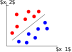
\includegraphics[width=0.5\columnwidth]{figs/linearlyseparable}
    \def\svgwidth{0.6\textwidth}
    \import{./figs/}{linearlyseparable.pdf_tex}
    \caption{A 2-dimensional dataset (every element has two values $x_1$ and $x_2$) consisting of two classes, red and blue, that can be separated by a straight line.\label{fig:linearsep}}
\end{figure}

Formally, a Perceptron has $m$ inputs, $x_1$ to $x_m$, each modulated by a weight $w_1$ to $w_m$, respectively, as well as a treshold $b$, and outputs either zero or one (\cref{fig:perceptron}). This is schematically illustrated in \cref{fig:perceptron}.

\begin{figure}[htb]
    \centering
    % 
\includegraphics[width=0.5\columnwidth]{figs/perceptron.png}
    \def\svgwidth{0.66\textwidth}
    \import{./figs/}{perceptron.pdf_tex}
    \caption{The simple perceptron passes the dot product between the inputs $x$ and weights $w$ through a Heaviside function, returning 1 when $wx+b>0$ and 0 otherwise.
    \td{Nikolaus, I don't think you are explaining well what this $\frac{b}{w_0}$ is, why there is a $w_0$ in the first place, and how the equation below is related to this picture.}}\label{fig:perceptron}
\end{figure}

The Perceptron classifies whether $x$ lies above or below a hyperplane defined by the weights $w$ using the following equation:
%
\begin{equation}
f(x)=\begin{cases}
1 \qquad wx+b > 0\\
0 \qquad otherwise
\end{cases}
\end{equation}
%
Here, $wx=\sum_{i=1}^mw_ix_i$ is the dot product and the non-linear activation function is also known as \index{Heaviside step function}\textsl{Heaviside step function}. In practice, we are appending the value of '1' to the vector $x$ so that $x_0=1$, which simplifies $wx+b$ to $wx$ where $w_0$ taking up the role of $b$. This is illustrated in \cref{fig:perceptron}, where the bias $b$ is alternatively labeled by $w_0$ and input $x_0=1$.


\subsection{Geometric interpretation of the simple perceptron}
If $w$ really defines a hyperplane, we should be able to see it when $m=2$. When $m=2$, that is every data point $x$ has only 2 dimensions, the separating hyperplane is a line. This can be seen as follows: writing the dot product out yields
\begin{equation}
w_1x_1+w_2x_2+b=0
\end{equation}
As we plot $x_1$ along the x-axis and $x_2$ along the y-axis, we can write
\begin{equation}
w_1x+w_2y+b=0
\end{equation}
This can be rewritten into
\begin{equation}
y=-\frac{w1}{w2}x-\frac{b}{w_2}
\end{equation}
and displayed within a scatter plot.

\subsection{Training the simple Perceptron}
Training the Perceptron, that is finding appropriate values for $w$ and $b$ that separate the data into two classes, is a simple iterative process:

\begin{enumerate}
\item Initialize the weights with zeros or a small random number
\item Compute the prediction $y_j=f(wx_j+b)$ for each data point $x_j$. A suitable choice for $f()$ is the Heaviside step function, e.g.
\item Calculate the mismatch between prediction $y_j$ and the true class $d_j$ to update the weights
\begin{equation}
w(t+1)=w(t)+r(d_j-y_j)*x_j
\end{equation}
\end{enumerate}

Repeat steps 2 and 3 until a termination criteria, such as a decreasing error or maximum number of iterations, is reached.

Albeit very simple, this simple learning algorithm has still a lot in common with state-of-the-art algorithms. First, weights are updated in an iterative process using small increments governed by a parameter $r$, standing for \index{Learning Rate}\textsl{learning rate}. By changing $w$ in small increments, the algorithm is literally rotating and translating the separating line in a direction that minimizes the \textsl{loss}, given by $d_i-y_i$. One can easily see that if the learning rate is too low, the algorithm will never find a good solution. One can also see that if the learning rate is too large, the line might move too much, skipping the optimal pose.

Notice that this simple implementation is de facto implementing gradient descent on a loss function of the form $(d_i-y_i)^2$, that can be minimized by moving against the direction of its gradient, here $2(d_i-y_i)$.

Second, the learning algorithm requires multiple presentations of the data-set, as the error is computed for every point in the data set. The more data, the longer training takes, in this case the increase in time is linear, which is a good approximation also for modern learning algorithms.

Third, the error between prediction and true class is only calculated based on training data. Even if we train with unlimited amounts of data points, it is still difficult to answer how the algorithm generalizes for new data, and whether also these new measurements will be distributed as the training data.

\section{Activation Functions}
Using a on-off Heaviside step function makes training a neural network using gradient descent rather difficult as a function that switches from ``not working at all'' to ``working completely'' provides very little information in which direction to move. It is therefore more desirable to have a smooth activation function. One such function is the \index{Sigmoid function}\textsl{sigmoid function}:
\begin{equation}
\sigma(x)=\frac{1}{1+e^{-x}}
\end{equation}
Its main characteristics are that it assymptotically stays between 0 and 1, and crosses the y-axis at 0.5. It is shown in \cref{fig:activationfunctions}, left.

\begin{figure}[htb]
    \centering
    % 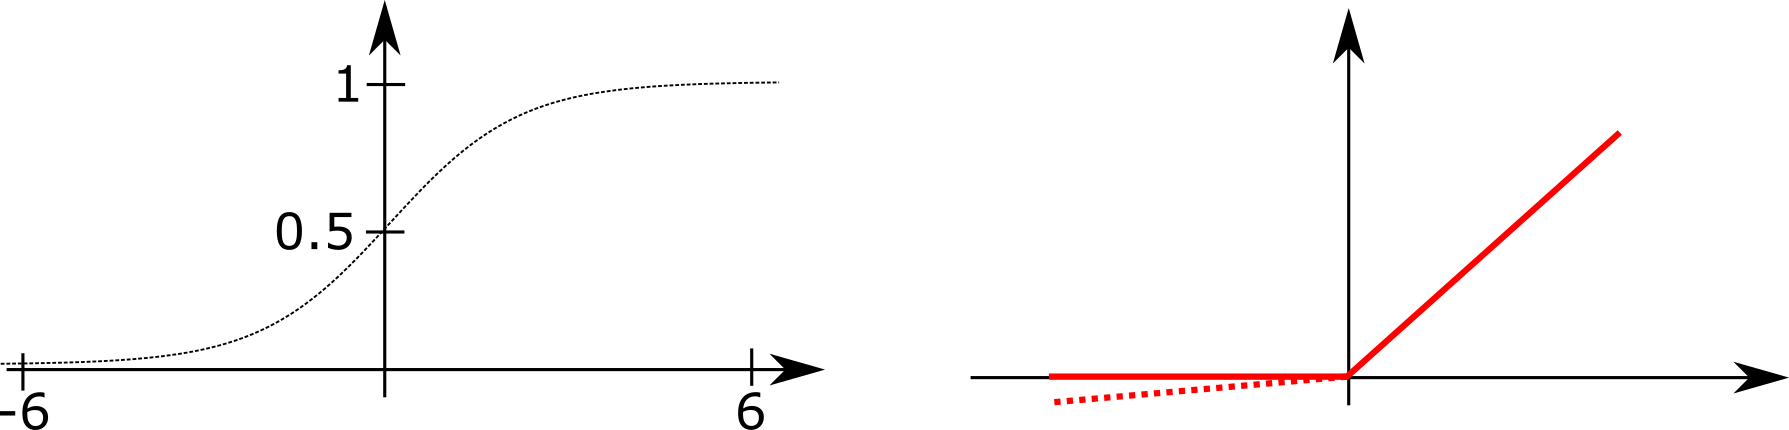
\includegraphics[width=0.9\columnwidth]{figs/activationfunctions}
    \def\svgwidth{0.9\textwidth}
    \import{./figs/}{activationfunctions.pdf_tex}
    \caption{Typical activation functions used in neural networks, the Sigmoid activation function, left, and the rectified linear unit (ReLU).\label{fig:activationfunctions}}
\end{figure}

The sigmoid function is very attractive for learning as the direction in which the weights should move to improve the error is very clear in the vicinity of $wx=0$, and computing its derivative is rather simple as we see below. In case of $wx$ being very large, or very small, the neuron either saturates or never activates, also known as the \textsl{vanishing gradient}problem. Another drawback is that computing the sigmoid function is computationally expensive. A similar function is the hyperbolic tangent $\tanh()$ which remains in the range of -1 to 1 and crosses the y-axis at 0.

A popular solution to decrease computation time is the \index{Rectified Linear Unit (ReLU)}\textsl{Rectified Linear Unit} (ReLU), which is given by
\begin{equation}
R(x)=max(0,x)
\end{equation}
and is shown in \cref{fig:activationfunctions}, right.The dashed line indicates a refinement of the ReLU known as \textsl{leaky ReLU} with a slope of typical 0.1, and improves learning for negative $wx$ by providing a directional gradient.

Note that we only talk about ``Perceptrons'' when the Heaviside step function is used as activation function.

\section{From the simple Perceptron to Multi-layer neural networks}

We have seen that the single Perceptron is able to linearly separate a dataset, spitting out ``0'' or ``1'' as a function of the data being below or above the separating hyperplane defined by the weight vector $w$. It is easy to see that some problems cannot be linearly separated. This is illustrated in \cref{fig:xorproblem}.

\begin{figure}[htb]
    \centering
    % 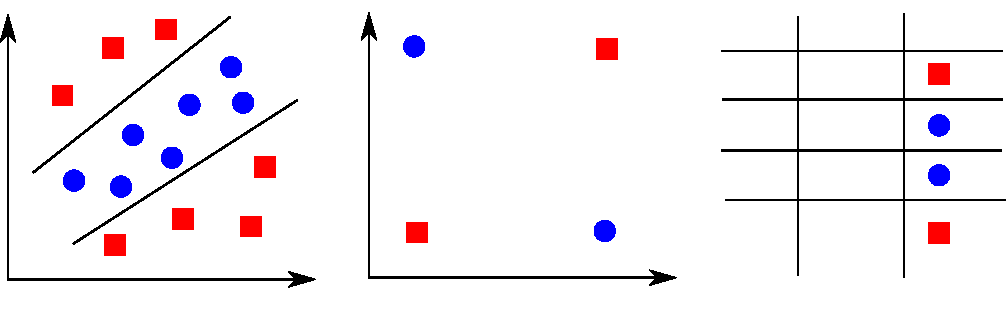
\includegraphics[width=0.9\columnwidth]{figs/xorproblem}
    \def\svgwidth{0.9\textwidth}
    \import{./figs/}{xorproblem.pdf_tex}
    \caption{Data that cannot be separated using a single line (left) in canonical form (center). This problem is known as the ``XOR'' problem due to the truth table of the associated classification problem (right).\label{fig:xorproblem}}
\end{figure}

In the example above, the red and the blue data points are not separable by a single line, but require at least two lines. This problem is known as the ``XOR'' problem, which can be seen by looking at just four data points at $(0,0)$, $(0,1)$, $(1,0)$, and $(1,1)$. Tabulating this data togethwer with its color, reveals a truth table with the characteristics of logical exclusive or (XOR), that is $x_1$ and $x_2$ have to be different for the output to be true (here ``blue''), whereas the output is false (here ``red'') when the inputs are the same.

We already know that a single Perceptron can create a single separating hyperplane, we will therefore need at least two Perceptrons to solve the XOR problem. Using two Perceptrons in parallel will yield us with tuples of the kind $(0,0)$, $(0,1)$ and so on. We therefore need one more Perceptron to recombine these tuples into a single output. \cref{fig:basicmultilayer}
shows the simple-most multi-layer Perceptron that can be trained for the XOR problem, with one \index{Input Layer}\textsl{input layer}, a so-called\index{Hidden Layer} \textsl{hidden layer}, and an \index{Output Layer}\textsl{output layer}.

\begin{figure}
    \centering
    % 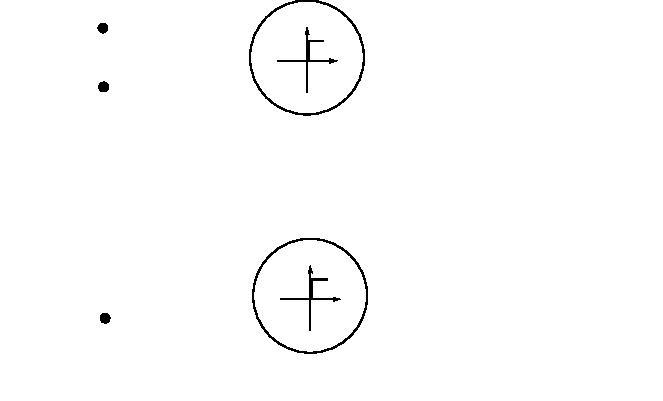
\includegraphics[width=0.8\columnwidth]{figs/basicmultilayernetwork}
    \def\svgwidth{0.8\textwidth}
    \import{./figs/}{basicmultilayernetwork.pdf_tex}
    \caption{A simple multi-layer perceptron with one input layer, one hidden layer, and one output layer. \label{fig:basicmultilayer}}
\end{figure}

\subsection{Formal description of Artificial Neural Networks}
As with the simple Perceptron, we will use node i's bias as the 0-th weight vector, that is
\begin{equation}
w^k_{0,j}=b^k_j
\end{equation}
Here, we use the following notation. We will denote the layer with a superscript, and the index of the incoming node and the outgoing node with a subscript tuple. That is $w^k_{i,j}$ is connecting the i-th incoming weight to the $j-th$ node of the $k-th$ layer. (The i-th incoming weight is the j-th node in layer $k-1$.) This, as well as the simple example network from above, are illustrated in \cref{fig:backpropnotation}.

\begin{figure}[htb]
    \centering
    % \includegraphics[width=0.7\columnwidth]{figs/backpropnotation}
    \def\svgwidth{0.7\textwidth}
    \import{./figs/}{backpropnotation.pdf_tex}
    \caption{Notation used to index weights (left) with respect to layer $k$ and the multi-layer network from \cref{fig:basicmultilayer} (right).\label{fig:backpropnotation}}
\end{figure}

Each layer, denoted by the index $k$, has exactly $r^k$ nodes.

\subsection{Inputs and outputs}

The output $o_i$ of output node $i$ is given by
\begin{equation}
o_i=g(a_i^k)
\end{equation}
where $g()$ is a non-linear activation function such as --- but not limited to --- the Heaviside step function. Here, $a_i^k$ is the weighted sum computed by node $i$ in layer $k$, also known as the \index{Activation (neural network)}\textsl{activation}:
\begin{equation}
a_i^k=\sum_{j=0}^{r_{k-1}}w_{j,i}^ko_j^{k-1}
\end{equation}
with $o_j^{k-1}$ the j-th output of the previous layer. This is illustrated in \cref{fig:backpropnotation2}.

\begin{figure}[htb]
    \centering
    % \includegraphics[width=0.7\columnwidth]{figs/backpropnotation2}
    \def\svgwidth{0.7\textwidth}
    \import{./figs/}{backpropnotation2.pdf_tex}
    \caption{Inputs and outputs of neuron $i$ in the $k$-th layer showing activation $a_i$ and output $o_i$.\label{fig:backpropnotation2}}
\end{figure}

In case of $k$ being the output layer, $o_i^k$ should be equivalent to $y_i^k$. Likewise, in case of $k-1$ being the input layer $o_i^{k-1}=x_i$.

\subsection{Training a multi-layer neural network}

Finding a set of weights and bias values, that is 9 parameters for a simple two-dimensional problem, but potentially millions for a ``deep network'', is an NP-complete problem \cite{blum1992training}. We therefore need a smart approximative algorithm. We consider a training dataset consisting of input-output pairs $x_i$ and ouput $y_i$ with $i=1..N$, and a feedforward neural network with parameters $w$.

\subsubsection{Loss function}
The goal of training is to minimize an error function such as the mean squared error
\begin{equation}
E(x,y,w)=\frac{1}{2N}\sum_{i=1}^{N}(\hat{y_i}-y_i)^2
\end{equation}
between the output $\hat{y_i}$ that the neural network with parameters $w$ computes and the known value $y_i$ from what is known as the \index{Training set}\textsl{training set}.

Similar to the Perceptron, we can reduce $E(x,y,w)$ by iteratively descending along its gradient, that is
\begin{equation}
w(t+1)=w(t)-\alpha \frac{\partial E(x,y,w(t))}{\partial w}
\end{equation}

\subsubsection{Backpropagation}
Calculating the partial derivatives for the error function manually is not straightforward as the neural network implements a computation graph, transforming the input $x$ by a series of multiplications and non-linear activation functions, which in turn require the chain rule.

Applying the chain rule can be done in two ways: moving forwards or backwards through the computation graph. Actually doing this by hand for a simple graph shows that going backwards is significantly more efficient. Manually deriving the individual partial derivatives also illustrates that many of the computations can actually be recycled. This solution is known as \index{Backpropagation}\textsl{backpropagation} \cite{rumelhart1985learning}, a technique that has been independently discovered in multiple fields. The derivation below follows \cite{backpropagation}.

In a first step, we note that the error function is a sum over all input-output pairs:
\begin{equation}
\frac{\partial E(x,y,w)}{\partial w_{i,j}^k}=\frac{1}{2N}\sum^N_{d=1}\frac{\partial}{\partial w_{i,j}^k}(\hat{y_d}-y_d)^2=\frac{1}{2N}\sum_{d=1}^N\frac{\partial E_d}{\partial w_{i,j}^k}
\end{equation}
We will therefore focus on only one input-output pair $(x_d,y_d)$ and differentiate against $w_{i,j}^k$. (The index $d$ has been chosen to avoid confusion with the indices $i$ and $j$, and will be omitted for brevity in the remainder).

\paragraph{The Chain rule} The key for understanding the backpropagation algorithm is to apply the chain rule in a correct way. Specifically, if a variable $z$ depends on the variable $y$, which itself depends on the variable $x$, then
\begin{equation}
\frac{dz}{dx}=\frac{dz}{dy}\frac{dy}{dx}
\end{equation}

With the output layer having index $m$ and a single output ($a^m_1$), the error is computed by the recursive formula
\begin{equation}
E(x,y,w_{i,j})=\frac{1}{2}(\hat{y}-y)^2=\frac{1}{2}(g(a_1^m)-y)^2=
\frac{1}{2}\left(g\left(\sum_{l=0}^{r_{m-1}}w_{l,1}^mo_l^{m-1}\right)-y\right)^2.
\end{equation}
We observe that the variable $E$ depends on the outputs $o_l^{m-1}$ with $l=0..r_{m-1}$ from the previous layer. Recall that $o_l^{m-1}$ is simply the activation $a_l^{m-1}$ after applying the activation function. Also recall that $w^m_{i,1}$ are weights coming into node $1$. The error with respect to $w_{i,j}$ is therefore dependent on all $a^k_j$ for all previous layers. This is also visualized in \cref{fig:backpropnotation3}.

\begin{figure}[htb]
    \centering
    % \includegraphics[width=0.8\columnwidth]{figs/backpropnotation3}
    \def\svgwidth{\textwidth}
    \import{./figs/}{backpropnotation3.pdf_tex}
    \caption{Last three layers of a neural network with a single output neuron, illustrating dependencies between function values and the output when moving along the computation graph backwards.\label{fig:backpropnotation3}}
\end{figure}

The chain rule therefore states
\begin{equation}
\frac{\partial E}{\partial w_{i,j}^k}=\frac{\partial E}{\partial a_i^k}\frac{\partial a_i^k}{\partial w_{i,j}^k}
\end{equation}

\paragraph{Error at layer k}
The first term is part of a vector called the ``error at layer $k$''  that consists of errors at all nodes $j$ in layer $k$ and is denoted by
\begin{equation}
\delta^k_j=\frac{\partial E}{\partial a_j^k}
\end{equation}

The second term can be computed from the definition of $a_j^k$ above
\begin{equation}
\frac{\partial a^k_j}{\partial w_{i,j}^k}=\frac{\partial}{\partial w_{i,j}^k}\left(\sum_{l=0}^{r_{k-1}} w_{l,j}^k o^{k-1}_l\right)=o^{k-1}_i
\end{equation}
which follows from the fact that only the term involving $o^{k-1}_i$ is the one where $l=i$. In case you expect the chain rule to apply further, remember that $o^{k-1}_i$ is actually not dependent on $w_{i,j}^k$, so you are done here.

Thus, the partial derivative of the error function $E$ with respect to weight $w_{i,j}^k$ is
\begin{equation}
\frac{\partial E}{\partial w^k_{i,j}}=\delta^k_jo^{k-1}_i.
\end{equation}

We can see that the error $E$ with respect to each individual weight $w_{i,j}^k$ in a layer $k$ depends on the output of the layers coming before that. This is intuitive, as information propagates through the network. We will now also show that the error term $\delta_j^k$ actually depends on the error at layers above $k$, that is stems from the error $\hat{y}-y$ that we ultimately want to minimize.

\paragraph{Backward propagation of error}

In order to show how the error term $\delta^k_i$ relates to the error  at the output layer, we will start working backwards. Let $m$ be the index of the output layer. We are also only considering a network with one output neuron, that is $j=1$. The error at this final layer $m$ is given by
\begin{equation}
E=\frac{1}{2}(\hat{y}-y)^2=\frac{1}{2}(g(a_1^m)-y)^2
\end{equation}
Using the chain rule $\frac{\partial E}{\partial w_{i,1}^m}=\frac{\partial E}{\partial a^m_i}\frac{\partial a^m_i}{\partial w^k_{i,1}}$ as before yields
\begin{equation}
\delta^m_1=\frac{\partial E}{\partial a^m_1}=(g(a^m_1)-y)g'(a^m_1)=(\hat{y}-y)g'(a^m_1)
\end{equation}
for the error at layer $m$ and
\begin{equation}
\frac{\partial a^m_1}{\partial w^k_{i,1}}=o_i^{m-1}.
\end{equation}

Together, these two result into
\begin{equation}
\frac{\partial E}{\partial w_{i,1}^m}=(\hat{y}-y)g'(a^m_1)o_i^{m-1}.
\end{equation}

We continue to use the chain rule to work backward along the computation graph. Specifically, the activation $a^k_j$ at node $j$ in layer $k$, with $1\leq k <m$ feeds into all nodes $l=1..r^{k+1}$ of layer $k+1$. Therefore, the error $\delta^k_j$ calculates to
\begin{equation}
\delta^k_j=\frac{\partial E}{\partial a^k_j}=\sum_{l=1}^{r^{k+1}}\frac{\partial E}{\partial a_l^{k+1}}\frac{\partial a_l^{k+1}}{\partial a^k_j}
\end{equation}

Using $\delta^{k+1}_l=\frac{\partial E}{\partial a_l^{k+1}}$, the above equation simplifies to
\begin{equation}
\delta^k_j=\sum_{l=1}^{r^{k+1}}\delta_l^{k+1}\frac{\partial a_l^{k+1}}{\partial a^k_j}
\end{equation}

Inspecting the computation graph or the definition of $a^k_j$, we recall that $a_l^{k+1}$ receives the output $g(a_j^k)$ from every node $j=1..r^k$ in layer $k$ via weight $w_{j,l}^{k+1}$, i.e.
\begin{equation}
a_l^{k+1}=\sum_{j=1}^{r^k}w_{j,l}^{k+1}g(a_j^k)
\end{equation}
allowing us to compute the partial derivative
\begin{equation}
\frac{\partial a_l^{k+1}}{\partial a^k_j}=w_{j,l}^{k+1}g'(a_j^k).
\end{equation}
This allows us to provide the error at node $j$ in layer $k$, also known as the <b>backpropagation formula</b>:
\begin{equation}
\delta^k_j=g'(a^k_j)\sum_{l=1}^{r^{k+1}}w_{j,l}^{k+1}\delta^{k+1}_l
\end{equation}

With this last part, we are able to define a recursive definition to calculate the desired error gradient with respect to all weights in the neural network:
\begin{equation}
\frac{\partial E}{\partial w_{i,j}^k}=\delta_j^ko_i^{k-1}=g'(a_j^k)o_i^{k-1}\sum_{l=1}^{r^{k+1}}w_{j,l}^{k+1}\delta_l^{k+1}.
\end{equation}

This computation can be executed layer by layer, starting from the output layer and working its way backward. This phase is computationally very similar to the forward phase and allows reusing all the activations and outputs that have been previously computed. As an extra goody, the derivative of the sigmoid function $\sigma'(x)=\sigma(x)(1-\sigma(x))$, resulting in
\begin{equation}
\frac{\partial E}{\partial w_{i,j}^k}=\delta_j^ko_i^{k-1}=g(a_j^k)(1-g(a_j^k))o_i^{k-1}\sum_{l=1}^{r^{k+1}}w_{j,l}^{k+1}\delta_l^{k+1}.
\end{equation}
and from there
\begin{equation}
\frac{\partial E}{\partial w_{i,j}^k}=\delta_j^ko_i^{k-1}=o_j^k(1-o_j^k)o_i^{k-1}\sum_{l=1}^{r^{k+1}}w_{j,l}^{k+1}\delta_l^{k+1},
\end{equation}
omitting the need to store $a_j^k$ in addition to $o_j^k$, reducing the memory requirements of the algorithm by half.

\subsubsection{Backpropagation algorithm}

Training a network now follows these simple steps:
\begin{enumerate}
\item Randomly initialize the network's weigths.
\item Compute the error for this network for each item in the training set and store the output from each layer (forward propagation).
\item Use the recursive formula for $\frac{\partial E}{\partial w^k_{i,j}}$ to compute the gradient of the error function with respect to each weight using the stored values of the output from forward propagation and calculate the average over the entire training set.
\item Repeat steps 2-3 for a fixed number of iterations or when the error becomes reasonably small.
\end{enumerate}

Fortunately, calculating the partial derivatives is not very hard in practice as there exist tools that automatically calculate the gradient along a computational chain in various programming languages (autograd, PyTorch, e.g.). These tools are at the core of modern machine learning frameworks and enable you to construct arbitrary network architectures without worrying about how to actually calculate the gradients. Yet, it is difficult to understand how these tools work and what their limitations are without understanding the derivation above.

\section{From single outputs to representing higher dimensional data}
Extending a neural network from one single output to multiple binary classifiers is straightforward, requiring only to increase the dimensionality of the output vector. How to represent numerical values, such as digits from 0-9 or characters from A-Z?


\paragraph{One-Hot Encoding}  A very common approach is known as \textsl{One-Hot Encoding (OHE)}. In OHE, $n$ discrete labels such as numbers or characters will be encoded as a binary vector of length $n$. To encode the $i-th$ element of a set of lables, this vector is zero except at position $i$. For example, to encode the characters 0..9, OHE would result into

\begin{eqnarray}
\nonumber
0 = (1,0,0,0,0,0,0,0,0,0)\\
\nonumber
1 = (0,1,0,0,0,0,0,0,0,0)\\
\nonumber
2 = (0,0,1,0,0,0,0,0,0,0)\\
\nonumber
3 = (0,0,0,1,0,0,0,0,0,0)\\
\nonumber
4 = (0,0,0,0,1,0,0,0,0,0)\\
\nonumber
5 = (0,0,0,0,0,1,0,0,0,0)\\
\nonumber
6 = (0,0,0,0,0,0,1,0,0,0)\\
\nonumber
7 = (0,0,0,0,0,0,0,1,0,0)\\
\nonumber
8 = (0,0,0,0,0,0,0,0,1,0)\\
\nonumber
9 = (0,0,0,0,0,0,0,0,0,1).
\end{eqnarray}

\paragraph{Softmax output} Whereas One-Hot Encoding transforms the training input into a discrete probability distribution, nothing in the neural network will ensure that the data will also come out like that. A sigmoidal activation function would insure that each value remains between 0 and 1, but a ReLU does not. We therefore need a final layer that ensures each output to be limited to the range 0 to 1 \textsl{and} the sum of all elements to be adding up to one. This is usually achieved using a so-called \textsl{Softmax} layer. The softmax function is given by
\begin{equation}
{\sigma (\mathbf {z} )_{j}={\frac {e^{z_{j}}}{\sum _{k=1}^{K}e^{z_{k}}}}} \quad for \quad j=1,\ldots,K
\end{equation}

That is, a vector $z \in \mathbb{R}^K$ will be turned into a K-dimensional vector, which j-th element is given by the above formula.

So, why not just normalizing with the actual values, i.e. using $z_j$ instead of $e^{z_j}$, or even easier, just using $\arg \max_j$ function to set the highest value of $z$ to 1 and leave the rest at zero? The reason is that each layer needs to remain differentiable for backpropagation to work. Yet, a brutal cut-off like the $\arg \max$ function would introduce is what we actually really want for the network to optimally match the training input. This is why the exponential function is used. It - literally - exponentially emphasizes larger values over smaller values, making the class with the highest probability stand out.

\section{Convolutional Neural Networks}

\section{Transfer learning}

\section{Embeddings}

\section{Recurrent Neural Networks}

\section{Exercises}
\begin{enumerate}
\item Implement the simple perceptron training algorithm and use it to find a separating hyperplane for simple data.
\item Find out how to implement the auto differentiation (or auto gradient) function in your favorite numerical package, e.g. \textsl{NumPy} or \textsl{PyTorch} to automatically calculate the derivative of your loss function.
\item Use a machine learning package of your choice to train a classifier for synthetic images such as the ``Ratslife'' landmarks. If you can, use a real robot to generate appropriate training data.
\item Select a simple 2D target, e.g. a cross on white background, and record images from different distances and angles. Can you train a CNN to predict these two quantities from your image?
\item Select a pre-trained image classifier from your preferred machine learning toolkit and use it as the basis to train your classifier for either landmark recognition or pose recognition. How does using a pre-trained classifier affect learning time and accuracy?
\item What kind of network architecture would you chose to track the robot's location (odometry) based on encoder inputs?
\item Download the ``Robot Execution Failures Data Set'' from the UCI machine learning repository. It contains time-series data from a robot's force-torque sensor as well as whether manipulation was successful. Define a recurrent neural network architecture for this data and train it.
\end{enumerate}



\chapter{Task execution}
In its most basic implementation, sensors and actuators can be directly tied to each other, making a computer obsolete. Such robots are purely reactive, thereby missing the ability to ``think'' or plan. In order to achieve more complex behavior, memory and state are needed to switch between different controllers and algorithms.

This chapter introduces these basic principles as well as their implementation, starting with basic reactive controllers (Section \ref{sec:braitenberg}), then introduces more advanced concepts that let the robot make basic ``if'' \ldots ``then'' decisions using ``Finite State Machines'' (FSM) in Sections \ref{sec:fsm} and \ref{sec:stateflow}, and finally introduces advanced concepts such as ``behavior trees'' and semantic planning in Sections \ref{sec:behaviortrees} and \ref{sec:strips}.

\section{Reactive control}\label{sec:braitenberg}
A large variety of robotic behaviors can be accomplished by directly connecting sensor input to actuator output. This can even be accomplished without using a computer, but by using analog electronics that provide appropriate conditioning. Simple autonomous robots using this concept have been demonstrated as early as 1953 \cite{walter1953living} and have become known as ``tortoises''. For example, by tying the output of a light sensor to a motor controller, the motor turns faster the brighter the light is. Using an inverse relationship, the motor turns slower the brighter the light is. When used in a differential wheel configuration with two motors and two light sensors, such a robot either drives toward or away from the light. Formally, we can express the light following behavior, also known as \emph{phototaxis}\index{Phototaxis}, by the following relationship between 
the left and right wheel speeds, $\dot{\phi_l}$ and $\dot{\phi_r}$, and  $\lambda_r$ and $\lambda_l$ the measurements of the right and left light sensors
\begin{eqnarray}\label{eq:simplereactive}
\dot{\phi_l}=a \lambda_r + b\\
\dot{\phi_r}=a \lambda_l + b
\end{eqnarray}
with $a$ a constant weight, and $b$ a bias term. We observe that the left wheel turns faster, the brighter the light shines on the right sensor. If the right light sensor receives more light than the left sensor, the right wheel will turn slower, resulting into a right turn, thereby exhibiting phototaxis behavior.

\todo{Include figure showing simple braitenberg vehicles}

A more complex behavior is obstacle avoidance. Assuming the output of an obstacle sensor to increase with the obstacle approaching, e.g. an infrared proximity sensor, we can use the same principle to compute the wheel speeds such that the obstacle is actively avoided. An example for a differential-wheel robot with eight infrared proximity sensors is given by
\begin{eqnarray}
\nonumber
\dot{\phi_l}&=&-6d_0-6d_1-19d_2-13d_3+94d_4+63d_5-50d_6-6d_7+b\\
\nonumber
\dot{\phi_r}&=&-6d_0+50d_1+63d_2+94d_3-22d_4-10d_5-6d_6-6d_7+b
\end{eqnarray}
%
% back, left {-0.06, -0.06}, 
% left {-0.06, 0.5}, 
% front, left {-0.19, 0.63}, 
% front, front, left{-0.13, 0.942}
% front, front, right {0.942, -0.22}, % left right motor
% front, right {0.63, -0.1}, 
% right {0.5, -0.06},  
% back, right {-0.06, -0.06},
%
with $d_0$ the left rearward sensing, the sensors being arranged clockwise, and $d_7$ the right rearward sensing sensor, arranged as on the E-Puck differential wheel robot \cite{mondada2009puck}, see also Figure \ref{fig:epucksensors}.

\todo{Add figure showing infrared proximity into sensors chapter and show non-linear properties.}

Behaviors such as phototaxis and obstacle avoidance can also be combined by simply adding them and weighing each input accordingly. This idea has been popularized by the neuroscientist Valentino Braitenberg who augmented this system with additional ideas around learning (changing the weights based on events such as collisions), natural selection (building robots with random weights and selecting those that perform best), and analogies to the human brain \cite{braitenberg1986vehicles}. Controllers of these kind are therefore often called ``Braitenberg''.

Indeed, the controllers above bear strong resemblance to artificial neural networks such as described in Chapter \ref{chap:anns}, and ``optimal'' values to obtain a certain behavior can be obtained using evolutionary computation \cite{floreano1998evolutionary} or by training a neural network that yields appropriate input/output pairs. 

There are various variants of the control architecture including the \emph{subsumption architecture} \cite{brooks1990elephants} and \emph{motor schemas} \cite{arkin1989motor} that propose variations of switching different components of a reactive controller on and off to obtain a certain behavior. While useful to achieve simple behaviors, these approaches are difficult to manage in practice, and are better managed by being embedded in high-level control frameworks. 

\subsection{Limitations of reactive control}
The limitations of a reactive control scheme can be illustrated when considering a robot that combines phototaxis and obstacle avoidance and getting stuck in a U-shaped obstacle. While obstacle avoidance will prevent the robot from hitting the obstacle, as soon as the way is clear, the robot will keep turning toward the light, thereby getting stuck in a loop. (Everyone has observed such behavior in simple insects such as flies or moths.)

\todo{Show a simple U-Obstacle}

In order to avoid this situation, the robot needs to memorize its previous state and switch behaviors accordingly. For example, in addition to the basic combined avoidance and following behavior (``avoid and follow''), we can introduce an additional term (``wall following') in which the robot uses its proximity sensors to maintain a constant distance to a wall. In order to switch from one to the other behavior, we need to change the constant gains into dynamic ones that change their value based on other observations the robot makes. For example, the robot could estimate its progress by monitoring whether its light sensor is constantly increasing, and if it is not, inhibiting phototaxis behavior and emphasizing wall following. 

While feasible and potentially realizable with simple analog electronics, designing reactive systems with time-dependent behavior and state becomes difficult to manage very quickly. It is therefore desirable to find discrete abstractions for different behaviors that can be easily managed and understood by a programmer.  
%
%
\section{Finite State Machines}\label{sec:fsm}
A simple form to switch between different behaviors is a so-called \emph{Finite State Machine} (FSM)\index{Finite State Machine}\index{FSM}. In a FSM, each state is associated with a specific controller. In practice, a FSM consists of a global variable that stores the current state and a series of ``if'' statements that contain the code that is associated with each state. For example, a FSM to perform phototaxis while avoiding U-obstacles could consist of two states: one that computes wheel-speeds that move the robot toward the light while avoiding obstacles, the other that computes the wheel-speeds that implement wall following behavior. Each state, except the final state, will also need to contain additional conditions to switch into another state. These are known as \emph{state transitions}\index{state transition}\index{transition (state)}. A FSM can be depicted graphically, as shown in Figure \ref{fig:fsm_example}.

\todo{Insert FSM figure}
\begin{figure}
\caption{A simple Finite State Machine (FSM) with two states, an initial state, state transitions, and conditions that trigger a state transition.}
\end{figure}

Formally, a FSM is defined by a Tuple $(\Sigma, S, s_0, \delta, F)$ where:
\begin{itemize}
\item $\Sigma$ is the input \emph{Alphabet}, a set of symbols that represent events that can trigger state transitions,
\item $S$ is a finite set of states,
\item $s_0$ is an initial state, an element of $S$, that is $s_i \in S$,
\item $\delta$ is the state-transition function $\delta: S \times \Sigma \rightarrow S$ that maps combinations of states in $S$ and symbols $x$ in $\Sigma$ to a new state in $S$, and
\item $F$ is the set of final states, a subset of $S$. 
\end{itemize}

Historically, this definition stems from FSM formally defining the working of a computer with a stream of symbols commands of an actual program. In robotics, symbols that trigger state transitions can be itself the result of complex computations. For example, a robot might switch to wall-following if it has not made actual progress toward its goal in some time and resume phototaxis once it reached a position that is closer to the light than it was before. 

In conjunction with a controller for each state, a FSM is called a \emph{Hybrid System}\cite{van2000introduction} as it combines both discrete (the state) and continuous (the controller outputs) variables. 

\subsection{Implementation}
A low-level robot controller is usually implemented as a loop with fixed loop time, for example 100ms for slow moving differential-wheel robots and 1ms for dynamical systems such as drones. At each start of the loop, the controller reads all sensors, then branches into the part of the code that corresponds to its current state, processes sensor information and computes actuator output, and finally sends the control commands to the actuators. 

Unlike a computer program that can process information as fast as possible, the robot controller needs to wait until sensor information are actually available, and actuator commands are executed, that is the robot has physically moved. As the robots keeps moving while computation is ongoing, it is important to run the main loop at a constant rate. As computation is usually much faster than the loop time, it might therefore be necessary to use an internal clock to wait until the loop time is expired. 


%@book{van2000introduction,
%  title={An introduction to hybrid dynamical systems},
%  author={Van Der Schaft, Arjan J and Schumacher, Johannes Maria},
%  volume={251},
%  year={2000},
%  publisher={Springer London}
%}



\begin{enumerate}
\item State is kept by a global variable
\item Robot program is executed in a loop, switch statement is used to enter different branches
\item Each state includes conditionals that set next state
\item Loop execution time is constant, usually done via sleep statements. This is important as odometry computations require a constant time to function.
\item FSMs are difficult to maintain. Adding a state requires modifiying the transitions of all states leading into that state and possibly also out of that new state.
\end{enumerate}

\section{Hierarchical Finite State Machines}\label{sec:stateflow}
\begin{enumerate}
\item FSMs are grouped into clusters, creating super-states
\item Also known as ``Statecharts'' \cite{harel1987statecharts}

\item State transitions between super states can be tied to states to the included FSM or be implicitely connected to all states of the included FSM, which allows to leave the super state from every state therein.
\item Super states can also be executed in parallel, providing  events that lead to state transitions in other FSMs
\item Robot control software like ROS, LCM or Yarp provide frameworks to implement asynchrnous hierarchical FSMs, allowing super-states to subscribe to messages published by other super-states as well as directly triggering state transitions across different processes running in parallel in a service model.
\item HFSM solve some of the problems of FSMs by increasing modularity, thereby simplifying programmability, but still have the problem that $N$ states can lead to $N^2$ state transitions, each of which need to be manually coded.
\end{enumerate}

\section{Behavior Trees}\label{sec:behaviortrees}
\begin{figure}
    \centering
    \begin{forest}
    {for tree={%
        minimum height = 4ex, 
        minimum width = 4ex, 
        draw, 
        parent anchor=south, 
        child anchor=north, 
        align=center
        }
    }
        [{\scriptsize Tilt Insert}\\ $\longrightarrow^*$
            [\scriptsize Rotate\\ $\theta_{tilt}$]
            [\scriptsize Move to\\ \scriptsize Contact \normalsize $-Z$]
            [\scriptsize Rotate\\ $-\theta_{tilt}-\delta \theta$]
            [\scriptsize Rotate\\ $\delta \theta$]
            [\scriptsize Hand at\\ $Z_{insert}$, ellipse]
        ]
    \end{forest}
    \caption{Tilt Insert Skill BT. The sequence first ..., then moves downwards until contact is made, rotates ... }
    \label{BTtilt}
\end{figure}

\begin{enumerate}
\item Programs are organized into nodes, each implementing certain functionality.
\item A node can have sub-nodes, like leafs of a tree, that are sequentially executed.
\item Each node can be \emph{running}, \emph{failed}, or \emph{successful}.
\item Execution within a node is triggered by a so-called \emph{tick} received by its parent node.
\item Nodes report their state back to their parent node.
\item A parent node issues ticks to its child nodes one by another, only moving to the next of its child nodes once the last one has returned \emph{successful}.
\item As long as a child node is returning \emph{running}, it continues to receive ticks.
\item If a node fails, this information can be processed by the parent node who either passes it up, or restart the sequence of child nodes.
\end{enumerate}

\section{Mission Planning}\label{sec:strips}
\begin{enumerate}
\item The original GPS algorithm: operations that transform a set of pre-conditions into a set of post-states, and search thereon
\item Mission planning with BTs
\end{enumerate}

\section{Exercises}

\begin{enumerate}
\item A differential wheel robot has three downward-facing light sensors at its tip. The sensors are spaced such that the robot can detect a black line on a white ground. Derive the equations for a line-following robot using the Braitenberg formalism.
\item Derive a control scheme that combines line following and obstacle avoidance. Discuss your choices assuming that the robot has to avoid obstacles at all cost. 
\item Use a robotic simulator of your choice to implement basic phototaxis and obstacle avoidance. 
\item Use a robotic simulator of your choice to implement basic wall-following behavior
\item Implement a simple finite state machine that combines obstacle avoidance, phototaxis and wall-following and is capable to escape from a U-shaped obstacle
\item A FSM implements the following behavior: perform photo-taxis until an obstacle is it; then perform wall-following for 10 time steps. Draw an appropriate Finite State Machine. How many states do you need?
\item A robot runs at a 100ms loop time. Performing sensor readings takes 3ms, odometry computations 15ms, and executing logic takes 30ms on average. Which of these operations is likely to fail if the task logic takes 80ms?
\item Formulate both a Finite State Machine and a Behavior tree for the game ``Rats Life'', label each state and conditional transition, and compare the two representations.
\end{enumerate}

\chapter{Mapping}
Mapping is the process of building representations of the environment for
either downstream consumption by autonomy algorithms or for informing humans.
Maps inform decision-making for planning and control algorithms by, for
example, providing information on the surfaces and obstacles, objects with
which the robot can interact, or topological information like how rooms are
connected with one another. If maps of an environment are already provided,
robots can build plans over them without having to build a map themselves;
indeed, they can even localize themselves within these maps simply by
collecting information \emph{in situ} and referencing that information against
prior maps. Mapping also provides humans with an appreciation for what the
robot \emph{sees}, thereby guiding designers or operators of robots with
information about what is possible or information available to the robot.
Therefore, mapinformation for both the purposes of autonomy and design is a
critical linchpin to operating in real environments.

When one considers the quantities of interest to be collected from an
environment, there are two distinct classes: metric (e.g., the physical extents
of an environment) and semantic (e.g., the type of room one is in, or objects
of interest within it). These two categories can inform one another, for
instance a door is typically of a particular height or width, but the inference
required to resolve information in these two classes is remarkably different.
Metric information is frequently resolved using geometric techniques with which
we have become familiar in Chapter \ref{chap:sensors}, whereas semantic
information is typically obtained through machine learning techniques. For the
purposes of this text, we will focus almost exclusively on the problem of
metric mapping due to the prevailing importance of this information as it
relates to robotic planners and localization, but semantic mapping is a rich
field with an increasing importance to developing robotic autonomy; 
greater distinctions between these types of maps will be discussed in
Section \ref{sec:maps}.

With respect to metric mapping, range sensors have emerged as one of the most
effective sensors to make robots autonomous. Range data can be collected into
``scans'' from a sensor, each of which consists of a list of points that we
term a point cloud. Point clouds makes the construction of a 3D model of the
robot's environment straightforward; measurements on the environment are
inherently metric and require no ``front-end'' processing, as images from a
camera might require to extract such information. Furthermore, sensors that
output point cloud data are both quite accurate and increasingly common on
robotic platforms: the Velodyne 3D automotive lidar sensor that combines 64
scanning lasers into one package was key in mastering the DARPA Grand
Challenge, and no team operated without lidars as part of their solution in the
recent DARPA Subterranean Challenge. So for both wide-area and close-corridor
operation, 3D lidar has become a standard. There is one hitch with lidars: most
of them are built out of rotating laser arrays, which means that a moving
sensor will collect information from the environment at different rotation
angles, thereby \emph{aliasing} the lidar measurements with the motion of the
sensor. This motion aliasing can be removed from the lidar data, but is
negligible if the motion of the sensor is slow enough. However, there are
sensors that provide range data without this limitation, such as RGB-D (color
plus depth) cameras.  Furthermore, 3D range data has become even more important
in robotics with the advent of cheap (priced at a tenth of the price of the
cheapest 2D laser scanner) RGB-D cameras. In this chapter we will largely
ignore the source of range data, and will instead focus on algorithms that
operate over these data.

The mapping problem itself also ranges from trivial (when localization is
perfect) to arbitrarily complex, performing the equivalent of cartography in
which the tasks of localizing oneself and mapping the environment are closely
intertwined. While the problem of ``simultaneous localization and mapping''
will be introduced in Chapter \ref{chap:slam}, Section \ref{sec:ICP} describes
one of the key algorithms that is used to infer relative pose between
consecutive measurements by a process known as scan matching. 

Point cloud data allows fitting of lines and planes using RANSAC, which can
serve as features in EKF-based localization, but can also be used for improving
odometry, loop-closure detection, and mapping. Point cloud data can also be
probabilistically fused into voxel occupancy grids and dense surface
representations, which inform planning and design. The goals of this chapter
are:

\begin{itemize}
    \item introduce the Iterative Closest Point (ICP) algorithm for matching point clouds as an example of sparse mapping;
    \item show how ICP can be improved by providing initial guesses via RANSAC;
    \item use point clouds to generate dense maps built through occupancy grids; and
    \item demonstrate RGB-D mapping, another dense mapping technique that results in surface representations.
\end{itemize}

\section{Map representations}\label{sec:maps}
In order to plan a path, we need to represent the environment digitally. We
differentiate between two complementary approaches: discrete and continuous
approximations. In a discrete approximation, a map is sub-divided into sections
of equal (e.g., a grid or hexagonal map) or differing sizes (e.g., rooms in a
building). The latter maps are also known as \textsl{topological maps} or
\textsl{graph-based maps}.\index{Topological map}\index{Graph-based map}
Discrete maps lend themselves well to a graph representation. Here, every
region of the map corresponds to a vertex (also known as a ``node''), which are
connected by edges if a robot can navigate from one vertex to the other. For
example a road-map is a topological map with intersections as vertices and
roads as edges, labeled with their length (\cref{fig:pathproblem}).
Computationally, a graph might be stored as an adjacency or incidence
list/matrix. A continuous approximation requires the definition of inner
(obstacles) and outer boundaries, typically in the form of a polygon, whereas
paths can be encoded as sequences of points defined by real numbers. Despite
the memory advantages of a continuous representation, discrete maps are the
dominant representation in robotics.

There is no one correct choice for choosing a map representation, and each
application might require a different solution that could utilize a combination
of different map types.

Discrete and continuous representations are often matched together in clever ways. For example, roadmaps for GPS systems are stored as topological maps that store the GPS coordinates of every vertex, but might also contain overlays of aerial and street photography. These different maps are then used at different stages of the path planning stage.


\section{Iterative Closest Point for Sparse Mapping}
In its simplest form, a map can be created from slices of 2D range data such as obtained from a laser scanner. In the absence of a precise estimate of motion between two measurements, for example provided by odometry or IMU measurements, the challenge is to associate subsequent scans. 

A standard solution to this problem is known as the \emph{Iterative Closest Point} (ICP)\index{Iterative Closest Point}\index{ICP} algorithm. It was presented in the early 1990s for registration of 3D range data to CAD models of objects. A more in-depth overview of what is described here is given in \cite{rusinkiewicz01}. The key problem can be reduced to finding the best transformation that minimizes the distance between two sets of measurements.

In robotics, ICP found an application to match scans from 2D laser range
scanners. For example, the transformation that minimizes the error between two
consecutive snapshots of the environment is proportional to the motion of the
robot. This is a hard problem as it is unclear, which points in the two
consecutive snapshots are ``pairs", which of the points are outliers (due to
noisy sensors), and which points need to be discarded as not all points overlap
in both snapshots. Stitching a series of snapshots together theoretically
allows to create a 2D map of the environment. This is difficult, however, as
the error between every snapshots --- similar to odometry --- accumulates.
The ICP algorithm also works in 3D where it allows to infer the change in 6D
pose of a camera and creation of 3D maps. In addition, ICP has proven useful
for identifying objects from a database of 3D objects. Furthermore, the ICP
algorithm can be used to stitch consecutive range images together to create a
3D map of the environment \cite{henry2010rgb}. 

Before providing a solution to the mapping problem, we will focus on the ICP algorithm to match two consecutive frames. Variants of the ICP algorithm can be broken down into six consecutive steps:
\begin{enumerate}
    \item Selection of points in one or both meshes or point clouds.
    \item Matching/Pairing these points to samples in the other point cloud/mesh.
    \item Weighting the corresponding pairs.
    \item Rejecting certain pairs.
    \item Assigning an error metric based on the point pairs.
    \item Minimizing the error metric.
%    \item Point Selection.
\end{enumerate}
Depending on the number of points generated by the range sensor, it might make sense to use only a few selected points to calculate the optimal transformation between two point clouds, and then test this transformation on all points. Depending on the source of the data, it also turns out that some points are more suitable than others as it is easier to identify matches for them. This is the case for RGB-D data, where SIFT features have been used successfully. This is also the case for planar objects with grooves, where sampling should ensure that angles of normal vectors of sampling points are broadly distributed. Which method to use is therefore strongly dependent on the kind of data being used and should be considered for each specific problem.

\paragraph{Matching Points}
The key step in ICP is to match a point to its corresponding point in a different measurement. For example, a laser scanner hits a certain point at a wall with its 67th ray. After the scanner has been moved by 10 cm, the closest hit on the wall to this point might have been by the 3rd ray of the laser. Here, it is actually very unlikely that the laser hits the exact same point on the wall twice, therefore introducing a non-zero error even for an optimal pairing. Prominent methods involve finding the closest point in the other point cloud or finding the intersection of the source points' normal with the destination surface (for matching point clouds to meshes). More recently, SIFT has allowed to match points based on their visual appearance. Similarly to sorting through SIFT features, finding the closest matching point can be accelerated by representing the point cloud in a k-d tree.

\paragraph{Weighting of Pairs}
As some pairs are better matches than others, weighting them in some principled way can drastically improve the quality of the resulting transformation. One approach is to give more weight to points that have smaller distances from each other. Another approach is to take into account the color of the point (in RGB-D images) or use the distance of their SIFT features (weighting pairs with low distances higher than pairs with high distances). Finally, expected noise can be used to weight pairings. For example, the estimates made by a laser scanner are much more faithful when taken orthogonally to a plane than when taken at a steep angle.

\paragraph{Rejecting of Pairs}
A key problem in ICP are outliers either from sensor noise or simply from incomplete overlap between two consecutive measurement frames. A common approach to deal with this problem is to reject pairings when one of the points lies on a boundary of the point cloud, as these points are likely to match with points in non-overlapping regions. As a function of the underlying data, it might also make sense to reject pairings with too high of a distance. This is a threshold-based equivalent to distance-based weighting as described above.

\paragraph{Error Metric and Minimization Algorithm}
After points have been selected and matched, and pairs have been weighted and rejected, the match between two point clouds needs to be expressed by a suitable error metric which will then need to be minimized. One straightforward approach for this is to consider the sum of squared distances between each pair. This formulation can often be solved analytically. Let
\begin{eqnarray}
A=\{a_1,\ldots,a_n\}\\
B=\{b_1,\dots,b_n\}
\end{eqnarray}
be point clouds in $ \mathbb{R}^n$. The goal is now to find a vector $ t \in \mathbb{R}^n$ so that an error function $ \phi(A+t,B)$ is minimized. In 6D (translation and rotation), an equivalent notation can be found for a transformation (see forward kinematics). An error function for the squared distance is then given by
\begin{equation}
\phi(A+t,B)=\frac{1}{n}\sum_{a \in A}\|a+t-N_B(a+t)\|^2
\end{equation}
Here $ N_B(a+t)$ is a function that provides the nearest neighbor of $ a$ translated by $ b$ in $ B$.  A key problem now is that the actual value of $t$ affects the outcome of the pairing. What might look like a good match initially often turns out not be the final pairing. A simple numerical approach to this problem is to find $ t$ iteratively.

Initially $t=0$ and nearest neighbors/pairings are established. We can now calculate a $ \delta t$ that optimizes the least-square problem based on this matching using any solver available for the optimization problem (for a least-square solution $ \delta t$ can be obtained analytically by solving for the minimum of the polynomial by setting its derivative to zero). We can then shift all points in $ A$ by $ \delta t$ and start over. That is, we calculate new pairings and derive a new $ \delta t$.  We can continue to do this, until the cost function reaches a local minimum.

Instead of formulating the cost function as a ``point-to-point'' distance, a ``point-to-plane'' has become popular. Here, the cost function consists of the sum of squared distances from each source point to the plane that contains the destination point and is oriented perpendicular to the destination normal. This particularly makes sense when matching a point cloud to a mesh/CAD model of an object. In this case there are no analytical solutions to finding the optimal transformation, but any optimization method (such as Levenberg-Marquardt) can be used.

\section{Octomap: dense mapping of voxels}
For mapping obstacles, the most common map is the \textsl{occupancy grid
map}\index{Occupancy grid map}. In a grid map, the environment is discretized
into \emph{voxels} of arbitrary resolution, e.g. 1cm x 1cm, upon which obstacles are
marked. In a probabilistic occupancy grid, grid cells can also be marked with
the probability that they contain an obstacle. This is particularly important
when the position of the robot that senses an obstacle is uncertain.
Disadvantages of grid maps are their large memory requirements as well as the
computational time required to traverse data structures with large numbers of
vertices. A solution to this is storing the grid map as a \textsl{k-d
tree}.\index{k-d tree (data structure)} A k-d tree recursively breaks the
environment into $k$ pieces, subject to a subdivision rule (e.g., only
subdivide a space if it is between 5-95\% occupied). For $k=4$, an area that
fits the subdividing criteria would be subdivided into four pieces. Each of
these pieces can again be subdivided into four pieces and so on, until the
maximum allowable resolution is reached or the subdivision criteria no longer
applies. These pieces can be stored in a graph with each vertex having four
children, corresponding to the four pieces the space represented by the vertex
is broken into, unless it is a leaf of the tree. This data structure is
attractive because not all vertices need to be broken down to the smallest
possible resolution. Instead, only areas which contain obstacles need to be
subdivided. A grid map containing obstacles and the corresponding k-d tree are
shown in \cref{fig:gridvskdtree}. To capture 3D data, this representation can
be extended to a 8-d tree, also known as \textsl{Octree}\index{Octree}. 


\begin{figure}
    \centering
    % \includegraphics[width=\textwidth]{figs/gridvskdtree.png}
    \def\svgwidth{\textwidth}
    \import{./figs/}{gridvskdtree.pdf_tex}
    \caption{A grid map and its corresponding quadtree (k-d tree).\label{fig:gridvskdtree}}
\end{figure}

The values of each entry in the k-d tree is the probability that the particularly
specified voxel is occupied. Note that this probability may be calculated
through any number of sensor models, such as absolute thresholding or using a
probabilistic field-of-view sensor model. Absolute thresholding determines
that a voxel is occupied if the absolute count of points measured
by the sensor within a voxel is greater than a threshold. An improvement on this is
to use a probabilistic model wherein a false positives
incidence rate and false negative incidence rate are used to calculate the probability
that a sensor's measurements indicate that a particular voxel is filled. Either way,
these techniques result in a map that is probabilistically fused over a sequence of
measurements to indicate filled and unfilled space in the form of a volumetric map.


\section{RGB-D mapping: dense mapping of surfaces}
While occupancy grid mapping using a technique such as Octomap is efficient for
planning, there are some drawbacks of this technique. First, it can be immediately
observed that the map voxels are of a fixed resolution and fundamentally cannot
resolve small obstacles at any smaller scale than that of the voxels; that is, small
obstacles will appear larger. Furthermore, high-frequency information within the voxel
that may be relevant to planning, such as surface curvatures, are unresolvable.
However, this information seems out of reach for any voxelized representation of
the environment. The resolution to this paradox is to populate the value of voxels
not with probability of a voxel's being occupied, but rather the \emph{most probable distance}
to the nearest surface. If for a particular range scan, a surface lies beyond a certain voxel,
that distance is positive, and if a surface lies in front of a certain voxel,
that distance is negative. See Figure \ref{fig:sdf} for an example of this
mathematical construction, which is known as a \emph{signed distance field} (SDF).
SDFs admits parameterization of \emph{surfaces} that can be probabilistically updated
over a sequence of scans of an environment. Note that the SDF provides an implicit
representation of a surface as can be seen in Figure \ref{fig:sdf}.


\begin{figure}
    \centering
    \includegraphics[width=0.5\textwidth]{figs/sdf.png}
    \caption{Schematic of the generation of an SDF based on 2D range data from a sensor.\label{fig:sdf}}
\end{figure}


The SDF can naturally represent multiscale obstacles, and provides an added
benefit for planning algorithms: it provides the distance to the nearest
obstacle at the same time! This is helpful as distance to obstacles can be used
as a risk metric in planning algorithms (i.e.\ it is often advantageous to
maintain maximal distance from obstacles over a trajectory, which can be easily
obtained from the SDF). There are two significant downsides of this technique,
however.  First, it requires highly accurate pose information, frequently
meaning ICP must be performed for each scan from the sensor. Second is that
implicit representation of surfaces do not admit straightforward visualizations
of the 3D maps. In order to accomplish this, a rendered is required to operate
on the SDFs, which result in maps such as \cref{fig:kintinuous}, which is using
the method of \cite{whelan2013robust}.  The resulting visualizations can be
surprisingly high-resolution even over coarse voxelization of the environment.
Together with RGB information, it is possible to create complete 3D walk
throughs of an environment.

\begin{figure}
    \centering
    \includegraphics[width=\textwidth]{figs/kintinous}
    \caption{Fused point cloud data from a walk trough of an office environment using ``Kintinious''. Picture courtesy of John Leonard.\label{fig:kintinous}}
\end{figure}


The problem with using ICP continuously to generate these maps is that errors
in each transformation propagate into the maps generation process in the form
of map drift. Here, the SLAM algorithm (Chapter
\ref{chap:slam}) can be used to correct previous errors
once a loop closure is detected, but the update of SDFs on the trigger of a loop
closure requires both the continuous retaining and global reprocessing of all
data used to generate the SDFs that would be effected by the loop closure, which
is a high price to pay.

%This form of RGB-D mapping uses a variant of ICP that is enhanced by SIFT features for point selection and matching. Maps are build incrementally. SIFT features, and their spatial relationship, are used for detecting loop closures. %Once a loop closure is detected, an additional constraint is added to the pose graph and a SLAM-like optimization algorithm corrects the pose of all previous observations.

As ICP only works when both point clouds are already closely aligned, which might not be the case for a fast moving robot with a relatively noisy sensor (the XBox Kinect has an error of 3cm for a few meters of range vs. millimeters in laser range scanners), RGB-D Mapping uses RANSAC to find an initial transformation. Here, RANSAC works as for line fitting: it keeps guessing possible transformations for 3 pairs of SIFT feature points and then counts the number of inliers when matching the two point clouds, one of which being transformed using the random guess.


\section*{Take-home lessons}
\begin{enumerate}
\item The challenge in mapping an environment originates from the uncertainty in both localization and sensing.
\item Techniques that are used to overcome uncertainty in localization and sensing can in turn be used to increase confidence in the former. For example, given robust features such as corners or walls, ICP results can be used to improve odometry estimates.
\item In the absence of reliable localization, the mapping problem turns into the simultaneous localization and mapping problem that is addressed in Chapter \ref{chap:slam}.
\end{enumerate}

\section*{Exercises}
\begin{enumerate}
\item Simulate a Lidar sensor in a simulator of your choice.Devise a grid-map structure that will allow you to draw the robot's position. Use the constant angular offset of your Lidar sensor and the pose of the robot to compute map coordinates for each reading.
\item Run a simulated robot in an obstacle course and record a map using your simulated Lidar. Implement the ICP algorithm described above to estimate the translation between consecutive scans and compare them with your odometry estimate. 
\item Use ICP to improve the robot's state estimate for different settings of wheel-slip in your simulation.  
\end{enumerate}

%!TEX root = ../book.tex
\chapter{Path Planning}\label{chap:pathplanning}

Path planning is an important primitive for both autonomous mobile robots and manipulators; it allows a robot to find a path between two points.
A \textsl{path}\index{Path} is formally defined as a set of poses from a starting configuration to an ending configuration that respect a set of specifications (for example, avoiding obstacles for a mobile base or respecting a specific force profile at the end effector of a manipulator). It differs from the concept of \textsl{trajectory}\index{Trajectory} in that a trajectory is the execution (i.e., parametrization) of a path over time.
Depending on the choice of the planning algorithm, a path could satisfy various degrees of optimality with respect to some criteria such as minimizing path length, minimizing turns, or minimizing the amount of braking.
Algorithms to find a shortest path are important not only for robotics applications, but also in network routing, video games, and understanding protein folding.

Path planning requires a suitable representation of the environment (e.g., the map introduced in \cref{chap:mapping}) and a perceptual understanding of the robot's location with respect to such representation---which will be treated in \cref{chap:localization}. We will assume for now that the robot is able to localize itself, is equipped with a map, and is capable of avoiding temporary obstacles on its way. The goals of this chapter are to:

\begin{itemize}
\item understand the difference between graph-based and sampling-based planning algorithms,
\item explain basic path planning algorithms ranging from Dijkstra, to A*, D* and RRT,
\item introduce variations of the path planning problem, such as coverage path planning.
\end{itemize}

\section{Graph-based planning algorithms}

The problem to find a ``shortest'' path from one vertex to another through a connected graph is of interest for multiple domains, most prominently network routing for the internet, where it is used to find an optimal route for a data packet.
The term ``shortest'' here is defined as the minimum cumulative edge cost, which could be physical distance (in a robotic application), delay (in a networking application), or any other metric that is relevant for the task. An example graph with arbitrary edge lengths is shown in \cref{fig:pathproblem}.

\begin{figure}[!htb]
    \centering
    % \includegraphics[width=0.6\textwidth]{figs/pathproblem}
    \def\svgwidth{0.6\textwidth}
    \import{./figs/}{pathproblem.pdf_tex}
    \caption{A generic path planning problem from vertex I to vertex VI. The shortest path is I-II-III-V-VI, and has length of $13$. \label{fig:pathproblem}}
\end{figure}

\subsection{Considerations about the robot embodiment}

In the vast majority of path planning algorithms, the robot is treated as a point-mass element with no volume. In order for a path to be executed on the robot, it is important to take into account the physical embodiment of the robot and its non-zero volumetric occupancy, which complicates the path planning process.
It is possible for the robot to be reduced to a point-mass while growing all obstacles by the length of the longest extension of the robot from its center (for a circular robot, its radius). This representation is known as \textsl{configuration space}\index{Configuration space} as it reduces the representation of the robot to its controllable degrees of freedom (e.g., its $x$ and $y$ coordinates in the plane for a robot capable of planar translation). An example is shown in \cref{fig:cspace}. The configuration space can now either be used as a basis for a grid map or a continuous representation.

\begin{figure}[!htb]
    \centering
    % \includegraphics[width=0.9\textwidth]{figs/configurationspace}
    \def\svgwidth{0.9\textwidth}
    \import{./figs/}{configurationspace.pdf_tex}
    \caption{A map with obstacles and its representation in configuration space, which can be obtained by growing each obstacle by the robot's extension. \label{fig:cspace}}
\end{figure}

\subsection{Dijkstra's algorithm}\index{Dijkstra's Shortest Path Algorithm}
\screencast{https://youtu.be/_lHSawdgXpI}{dijkstra}

One of the earliest and simplest algorithms for path planning is Dijkstra's algorithm \cite{dijkstra1959note}. Given a map, Dijkstra is an iterative process where, starting from the initial starting configuration, the algorithm marks all its direct neighbors with the (possibly unitary) cost to reach them. It then proceeds to inspect the neighboring vertex with the lowest cost and all its adjacent vertices and marks them with the cost to get to them via the vertex under consideration. Once all neighbors of a vertex have been checked, the algorithm proceeds to the vertex with the next lowest cost. Once the algorithm reaches the goal vertex, it terminates and the robot can follow the edges pointing towards the lowest edge cost.

In the example in \cref{fig:pathproblem}, Dijkstra would first mark nodes II, III and IV with cost $3$, $5$ and $7$ respectively. It would then continue to explore all edges of node II, which so far has the lowest cost. This would lead to the discovery that node III can actually be reached in $3+1<5$ steps, and node III would therefore be relabeled with cost $4$. In order to completely evaluate node II, Dijkstra needs to evaluate the remaining edges before moving on and label node VI with $3+12=15$.
%
The node with the lowest cost is now node III (cost of $4$). We can now relabel node VI with $14$, which is smaller than 15, and label node V with $4+5=9$, whereas node IV remains at $4+3=7$. Although we have already found two paths to the goal, one of which better than the other, we cannot stop as there still exist nodes with unexplored edges and overall cost lower than $14$. Indeed, continuing to explore from node V leads to a shortest path I-II-III-V-VI of cost $13$, with no remaining nodes to explore.

As Dijkstra would not stop until there is no node with lower cost than the current cost to the goal, we can be sure that a shortest path will be found if it exists. We can therefore say that Dijkstra is both \textsl{complete} and optimal.\index{Complete (algorithm)}

As Dijkstra will always explore nodes with the least overall cost first, the environment is explored comparably to a wave front originating from the start vertex, eventually arriving at the goal. This is of course highly inefficient, in particular if Dijkstra is exploring nodes away from the goal.
As an example, if we were to add a couple of nodes to the left of node I in \cref{fig:pathproblem}, Dijkstra would explore all of these nodes until their cost exceeds the lowest found for the goal. This can also be seen when observing Dijkstra's algorithm on a grid, as shown in \cref{fig:dijkstragrid}.

\begin{figure}[htb]
    \centering
    % Note: fonts were not converted to latex here because it was messing around with sizes and everything looked bad.
    \includegraphics[width=\textwidth]{figs/dijkstragrid.pdf}
    % \def\svgwidth{0.9\textwidth}
    % \import{./figs/}{dijkstragrid.pdf_tex}
    \caption{Dijkstra's algorithm finding a shortest path from `S' to `G' assuming the robot can only travel laterally (not diagonally) with cost one per grid cell. Note the few number of cells that remain unexplored once the shortest path (grey) is found, as Dijkstra would always consider a cell with the lowest path cost first.\label{fig:dijkstragrid}}
\end{figure}

\subsection{A*}\label{sec:astar}\index{A* Shortest Path Algorithm}

Instead of exploring in all directions, knowledge of an approximate direction of exploration to reach the goal may help avoiding the exploration of nodes that are not needed to succeed in the task.
As humans, we can easily interpret the task in \cref{fig:dijkstragrid} and understand that most states in the top-left and bottom-right corner should not be explored if we want to find a solution in a short amount of time.
Such knowledge may be encoded in the search algorithm via a \textsl{heuristic function}\index{Heuristic function}, i.e. an informed guess or estimate of sorts. For example, we could give priority to nodes that have a lower estimated distance to the goal than others.
For this, we would mark every node not only with the actual distance that it took us to get there (as in Dijkstra's algorithm), but also with the estimated cost to target, for example by calculating the Euclidean distance or the \textsl{Manhattan distance}\index{Manhattan distance} between the vertex we are looking at and the goal.
This algorithm is known as A* \cite{hart1968formal}, and illustrated in \cref{fig:astargrid} using the Manhattan distance metric. Depending on the environment, A* might accomplish search much faster than Dijkstra's algorithm, and performs the same in the worst case.

\screencast{https://commons.wikimedia.org/wiki/File:Astar_progress_animation.gif}{astar}

\begin{figure}[htb]
    \centering
    % Note: fonts were not converted to latex here because it was messing around with sizes and everything looked bad.
    \includegraphics[width=\textwidth]{figs/astargrid.pdf}
    % \def\svgwidth{0.9\textwidth}
    % \import{./figs/}{configurationspace.pdf_tex}
    \caption{Finding a shortest path from `S' to `G' assuming the robot can only travel laterally (not diagonally) with cost one per grid cell using the A* algorithm. Much like Dijkstra, A* evaluates only the cell with the lowest cost, but takes an estimate of the remaining distance into account.\label{fig:astargrid}}
\end{figure}

An extension of A* that addresses the problem of expensive re-planning when obstacles appear in the path of the robot is known as D*\index{D*} \cite{stentz1994optimal}. Unlike A*, D* starts from the goal vertex and has the ability to change the costs of parts of the path that include an obstacle. This allows D* to re-plan around an obstacle while maintaining most of the already calculated path.

A* and D* become computationally expensive when either the search space is large, e.g., due to a fine resolution required for the task, or when the dimensions of the search problem are high (e.g. when planning for an arm with multiple degrees of freedom). Solutions to these problems can be provided by sampling-based path planning algorithms---that are described further below.

\section{Sampling-based Path Planning}

The previous sections have introduced a series of complete algorithms for the path planning problem, algorithms that are guaranteed to (eventually) find a solution if it exists. However, complete algorithms are often infeasible when the possible state space is large, due to practical limitations like available memory or time to execute the algorithm. This is often the case for robots with many degrees of freedom such as arms. In practice, most algorithms are only \textsl{resolution complete}\index{Resolution complete}, meaning they are only complete if the choice of environment resolution is fine enough, as the state-space needs to be somewhat discretized for them to operate and some solutions might be missed as a function of the resolution of the discretization.

Instead of evaluating all possible solutions or using a non-complete Jacobian-based inverse kinematic solution, sampling-based planners create possible paths by using random sampling as the basis for adding points to a tree until some solution is found or time expires. As the probability to find a path approaches one when the number of samples goes to infinity, sampling-based path planners are \textsl{probabilistic complete}\index{Probabilistic complete}. Prominent examples of sampling-based planners are \textsl{Rapidly-exploring Random Trees} (RRT)\index{Rapidly-exploring Random Tree}\index{RRT}\cite{lavalle1998rapidly} and \textsl{Probabilistic Roadmaps}\index{Probabilistic Roadmaps}\index{PRM}(PRM) \cite{kavraki1996probabilistic}. An example execution of RRT for an unknown goal, thereby reducing the continuous path planning problem to a discrete search problem, is shown in \cref{fig:rrt}.

\begin{figure}
    \centering
    \includegraphics[width=\textwidth]{figs/irrt}
    \caption{Counterclockwise from top-left: Random exploration of a 2D search space by randomly sampling points and connecting them to the graph until a feasible path between start and goal is found.\label{fig:rrt}}
\end{figure}

This example illustrates how a sampling-based planner can quickly explore a large portion of space and refine a solution as time goes on. Whereas RRT can be understood as growing a single tree from a robot's starting point until one of its branches hits a goal, probabilistic road-maps create a tree by randomly sampling points in the state-space, testing whether they are collision-free, connecting them with neighboring points using paths that are achievable subject to the kinematics of the robot, and then using classical graph shortest path algorithms to find shortest paths on the resulting structure. The advantage of this approach is that such a probabilistic roadmap has to be created only once (assuming the environment is not changing) and can then be used for multiple queries. PRMs are therefore a \textsl{multi-query} path planning algorithm.\index{Multi-query (path planning)} In contrast, RRTs are known as \textsl{single-query}\index{Single-query (path planning)} path planning algorithms.

In practice, the boundary between the different historic algorithms has become very diffuse, and single-query and multi-query variants of both RRT and PRM exist. It is important to note that there is no `silver bullet' algorithm or heuristic and even their parameter-sets are highly problem-specific. We will therefore limit our discussion on useful heuristics to those that are common to sampling-based planners.

\subsection{Rapidly Exploring Random Trees}
 \screencast{https://youtu.be/Ob3BIJkQJEw}{rrt}
Let $ \mathcal{X}$ be a $ d$-dimensional state-space. It can be helpful to think of this as either the robot's state given in terms of translation and rotations (6 dimensions), a subset thereof, or the joint space with one dimension per joint. Let $ \mathcal{G} \subset \mathcal{X}$ be a  d-ball (d-dimensional sphere) in the state-space that is considered to be the goal, max\_dist the longest permissible edge length, $t$ the allowed time, $k$ the maximum number of vertices to allow in the tree, and goal\_bias the percentage of the time the algorithm should try to connect to a goal state. An RRT planner would proceed as follows:


\begin{verbatim}
Tree=Init(X, G, start, max_dist, t, k, goal_bias);
iteration = 0
WHILE (ElapsedTime() < t AND iteration < k 
AND NoGoalFound(Tree,G)) DO
 iteration = iteration + 1
 IF RandomPercentage() < goal_bias THEN
  q_rand = SampleRandomGoal(G);
 ELSE
  q_rand = SampleRandomState(X);
 ENDIF
 q_nearest = NearestVertex(q_rand)
 q_new = Extend(q_nearest, q_rand, max_dist)
 edge = CreatePath(q_nearest, q_new);
 IF IsAllowablePath(edge) THEN
  Tree.addVertex(q_new);
  Tree.addEdge(edge);
 ENDIF
ENDWHILE
return Tree
\end{verbatim}

This process can be repeated on the resulting tree as long as time allows, and can be implemented with a subset of the input parameters provided above (e.g., without a maximum number of vertices, a maximum timeout duration, or a goal\_bias). RRT is known as an \index{Anytime algorithm} \textsl{Anytime} algorithm, since the algorithm being interrupted will still provide some kind of solution (in this case, a partial graph discretization of the state space). Given a suitable distance metric, the path cost can be stored at each node of the tree, allowing for tracking the shortest path to goal in case there are multiple vertices in the goal region.
%the cost-to-goal can be stored at each node of the tree (much easier if growing the tree from the goal to start), which allows retrieving the shortest path easily. 
There are four key points in this algorithm:

\begin{enumerate}
    \item Finding the next point to add to the tree (SampleRandomGoal, SampleRandomState, and Extend).
    \item Finding out where and how to connect this point to the tree taking into account the robot kinematics (NearestVertex, CreatePath).
    \item Testing whether this path is suitable, i.e., collision-free. (IsAllowablePath)
\end{enumerate}

A prominent method is to pick a random point in the state-space and connect it to the closest existing point in the tree or to the goal, as implemented above. This can require iterating over all nodes in the tree and calculating their distance to the candidate point. Clever selection of data structure for storing the graph can mitigate these costs to be sub-linear in the number of vertices on average. Other approaches put preferences on nodes with fewer out-degrees (those which do not yet have very many connections) and choosing a new point within its vicinity in the direction of the sampled point to add. Both approaches make it likely to quickly explore the entire state-space. Once a new point is sampled, the Extend function uses the max\_dist parameter to limit the maximum edge length, replacing q\_rand with a point on the line connecting q\_nearest and q\_rand that is max\_dist away from q\_nearest.

If there are constraints imposed on the robot's path, for example if the robot needs to hold a cup and therefore is not supposed to rotate its wrist, this dimension can simply be taken out of the state-space.

Once a possible path is found, the space to be sampled from can be reduced to the ellipsoid that bounds the maximal path-length. This ellipsoid can be constructed by mounting a wire of the maximum path length between start and goal and pushing it outward with a pen. Intuitively, only points that are contained by this ellipsoidal area can provide a shorter path than the one currently known, so it is unproductive to attempt to grow the tree elsewhere. This approach is particularly effective when running multiple copies of the same planner in parallel and exchanging the shortest paths once they are found \cite{otte2012}.

\subsection{Connecting Points to the Tree}
A new point is classically connected to the closest point already in the tree or to the goal. This can be done by calculating the distance to all points already in the tree. This does not necessarily generate the shortest path, however. RRT*\index{RRT*} offers a solution to this problem, and is an algorithm that grows the tree in a way that always minimizes the overall path length from the root to every vertex. This is done in two steps: first by connecting new vertices in an optimal way and second by rewiring the tree to make use of this new vertex. By considering all points in the tree within a d-ball (on a 2D map, $d=2$, a circle) from a fixed radius from each added vertex and finding the point that minimizes the overall path length to the start (instead of simply the nearest vertex), we can guarantee that the new vertex is connected on the shortest reachable path from the root of the tree. In the rewiring step, vertices near the newly added vertex are checked to see if an edge from the new vertex to them would result in a shorter path than from their current parent vertex. If this is true, and the edge is allowable (i.e., not in collision or within the physical abilities of the robot), the graph is rewired so the existing vertex is connected with the new vertex as its parent, and it's previous parent edge is removed.

Adding a point to the tree is also a good time to take into account the specific kinematics of a robot, for example a car. Here, a local planner can be used to generate a suitable trajectory that takes into account the orientation of the vehicle at each point in the tree.

\subsection{Collision Checking}
Efficient algorithms for testing collisions deserve a dedicated section. While the problem is intuitive in configuration-space planning in 2D (the robot reduces to a point) and can be solved using a simple point-in-polygon test, the problem is more involved for manipulators that are subject to self-collision.

As collision checking takes up to 90\% of the execution time in the path planning problem, a successful method to increase computational speed is ``lazy collision evaluation''\index{Lazy collision avoidance}. Instead of checking every point for a possible collision, the algorithm first finds a suitable path. Only after does it check every segment of this path for collisions. Segments in collision are deleted and the algorithm continues, but it only keeps the segments of the successful path that were collision-free.

\section{Path Smoothing}
As paths are randomly sampled, they will be most likely shaky and not optimal. For example, a grid-map will generate a series of sharp turns and a sampling-based approach will return zig-zagging paths. Results can be drastically improved by running an additional algorithm that smooths the path. One way of doing this is to connect points of the path using splines, curves, or even trajectory snippets that are known to be feasible for a specific platform. Alternatively, one can also use a model of the actual platform and use a feedback controller such as described in Section~\ref{sec:fbmobile} for mobile robots and Section~\ref{sec:kinematics:inverse:arm} for arms, sample a series of points in front of the robot, and generate a trajectory that the robot can actually drive. When combined with dynamics, this approach is known as \textsl{model-predictive control}\index{Model-predictive control}. Care needs to be taken, however, that the resulting paths are indeed collision free.

\section{Planning at different length-scales}
In practice, no one map representation and planning algorithm might be sufficient. Planning a route for a car, for example, might involve a coarse search over the street network (like one performed by your preferred mapping and navigation app), but not involve planning which lane to actually choose. Planning lanes and how to navigate round-abouts and intersections will necesitate another layer of discrete planning. It may even be preferable to use a sampling-based algorithm to determine how to actually move the robot within a lane and avoid local obstacles. Finally, trajectories need to be turned into wheel speeds and steering angles, possibly using some form of feedback control. This hierarchy is depicted in \cref{fig:planninglayers}. Here, downward-pointing arrays indicate input that one planning layer provides to the one below. Upward-pointing arrows instead indicate exceptions that cannot be handled by the lower levels. For example, a feedback controller cannot handle obstacles well, requiring the sampling-based planning layer to come up with a new trajectory. Should the entire road be blocked, this planner would need to hand-off control the lane-based planner. A similar case can be made for manipulating robots, which also need to combine multiple different representations and controllers to plan and execute trajectories efficiently.

\begin{figure}
    \centering
    % Note: fonts were not converted to latex here because it was messing around with sizes and everything looked bad.
    \includegraphics[width=\textwidth]{figs/planninglayers.pdf}
    % \def\svgwidth{0.9\textwidth}
    % \import{./figs/}{planninglayers.pdf_tex}
    \caption{Path planning across different length-scales, requiring a variety of map representations and planning paradigms. Arrows indicate information passed between layers.\label{fig:planninglayers}}
\end{figure}

Note that this representation does not include a reasoning level that encodes traffic rules and common sense. While some of these might be encoded using cost-functions, such as maximizing distance from obstacles or insuring smooth riding, other more complex behaviors such as adapting driving in the presence of cyclists or properties of the ground need to be implemented in an additional vertical layer that has access to all planning layers.


\section{Other path planning applications}

Once the environment has been discretized into a graph, we can employ other algorithms to plan desirable robot trajectories. For example, floor coverage can be achieved by performing a depth-first search (DFS) or a breadth-first-search (BFS) on a graph where each vertex has the size of the coverage tool of the robot. ``Coverage'' is not only interesting for cleaning a floor: the same algorithms can be used to perform an exhaustive search of a configuration space, such as in the example shown in \cref{fig:inversekinematics}, where we plotted the error of a manipulator arm in reaching a desired position over its configuration space. Finding a minimum in this plot using an exhaustive search solves the inverse kinematics problem. Similarly, the same algorithm can be used to systematically follow all links on a website till a desired depth (or actually retrieving the entire world-wide web).

Doing a DFS or a BFS might generate efficient coverage paths, but they are far from optimal as many vertices might be visited twice. A path that connects all vertices in a graph but passes every vertex only once is known as a \textsl{Hamiltonian Path}.\index{Hamiltonian Path} A Hamiltonian path that returns to its starting vertex is known as a Hamiltonian Cycle. This problem is also known as the Traveling Salesman Problem (TSP), in which a route needs to be calculated that visits every city on his tour only once and is known to be NP Complete.\index{Traveling Salesman Problem}


\section{Summary and Outlook}
Path planning is an ongoing research problem. Finding collision free paths for mechanisms with high degrees of freedom such as multiple arms operating in a common space, multi-robot systems, or systems involving dynamics (and therefore adding the derivatives of the state variables to the planning problem) might take unacceptably long to solve.

Although sampling-based path planners can drastically speed up the time to find some solution, they are not optimal and struggle with specific situations such as narrow passages. There is no ``silver bullet'' algorithm for solving all path planning problems and heuristics that lead to massive speed-up in one scenario might be detrimental in others. Also, algorithmic parameters are mostly ad-hoc and correctly tuning them to a specific environment might drastically increase performance.


\section*{Take-home lessons}
\begin{itemize}
\item The first step in path planning is choosing a map representation that is appropriate to the application.
\item The second step is to reduce the robot to a point-mass, which allows planning in the configuration space.
\item This allows the application of generic shortest path finding algorithms, which have applications in a large variety of domains, not limited to robotics.
\item A sampling-based planning algorithm finds paths by sampling random points in the environment. Heuristics are used to maximize the exploration of space and bias the direction of search. This makes these algorithms fast, but neither optimal nor complete.
\item As the resulting paths are random, multiple trials might lead to totally different results.
\item There is no one-size-fits-all algorithm for a path planning algorithm and care must be taken to select the right paradigm (single-query vs.\ multi-query), heuristics, and parameters.
\end{itemize}

\section*{Exercises}\small
\begin{enumerate}
\item How does the computational complexity of Dijkstra's algorithm change when moving from 2D to 3D search spaces?
\item A* uses a ``heuristic'' to bias the search in the expected direction of the goal. Why can it only use a heuristic, not the actual length?
\item Assuming points are sampled uniformly at random in a randomized planning algorithm. Calculate the limiting behaviour of the following ratio (area of points in tree)/(area of points sampled) as the number of points sampled goes to infinity, assuming no duplicates. Assume the total area $A_{total}$ and the area of free space $A_{free}$ within are known.

\item Assuming a kd-tree is used as a nearest-neighbour data structure, and points are sampled uniformly at random, calculate the  run-time of inserting a point into a tree of size $N$. Use ``big-Oh'' notation, e.g. $\mathcal{O}(N)$.

\item What other practical runtime concerns must one consider besides computational complexity alone when doing sampling based motion planning? Can you suggest ways to deal with these other concerns?

\item Write a program that can read in a simple map provided as a textfile where '1' indicate obstacles and '0' indicates free space.
\begin{enumerate}
\item Implement Dijkstra's algorithm to find the shortest path between any two given points in free space.
\item Implement A* to find the shortest path between any two given points.
\item How do these two implementations compare in terms of computational complexity?
\end{enumerate}
\item Write a program that can read an image file in which white areas represent navigable space and black obstacles. Implement a basic RRT algorithm to find the shortest path between any two points.
\item Explore the internet for libraries that implement ``path planning'' in the language of your choice. What tools do you find? How do they define the map? Do they performan obstacle avoidance? Does the kinematics of the robot matter?
\item Extend your path planning implementation for being used with a differential wheel robot. Describe steps that you would need to take for Dijkstra/A* and for RRT.
\item Extend your path planning algorithm for being used with a two-link robot arm. Would you plan in joint or in configuration space, and what are advantages and drawbacks of each?
\item How does the computational complexity change when moving from a single 6-DoF robot arm to a torso with two 6-DoF robots? Can you think about an approach that maintains the original computational complexity? What are the drawbacks of this approach.
\item Consider a robotic assembly task in which a robot retrieves objects from a known location and assembles them on a table. When can you rely on simple inverse kinematics and when do you need path planning?
\item How does a planning problem change when you not only consider positions, but also forces and torques? Could you use  a variation of RRT to solve such a problem?
\item Download a robotic path planning tool that allows you to try different algorithms.
\begin{enumerate}
\item Compare solution quality and speed among the different solutions.
\item What do you need to take into account when using randomized planners? Is comparing single-shot experiments sufficient?
\end{enumerate}
\end{enumerate}

\normalsize

\chapter{Grasping and Manipulation Planning}\label{chap:manipulation}

While grasping is only concerned with attaching an object to a robot's kinematic chain, it is often the case that such an object is not just placed or dropped, but that the intention of the grasping action was to change the pose of this object in some meaningful way. For example, cutlery and dishes on a table need to be in well-specified areas and aligned with each other, merchandise needs to be neatly stacked in a shelf, and machine parts need to be assembled with each other. These activities are known as \textsl{manipulation}. Discussing all the possible ways objects might be manipulated, for example inserted, screwed-in, turned, twisted, flipped, etc., and the many different contexts such actions would be required --- which might dramatically change the approach a robot would need to chose --- are well beyond the scope of this book.

Yet, many manipulation problems can be cast into a sequence of grasping and placing problems in which the possible grasp choices are appropriately constrained. For example, an object can be turned or flipped by planning a sequence of pick-and-place movements that each turn the object by a certain degree. Similarly, using two robotic arms, with one grasping an object out of the hand of the other, will allow a robot system to change an object's pose almost arbitrarily. (Which poses an object will be able to reach will depend on the object's exact geometry, the kinematics of the robotic arms, and constraints in the workspace.) So-called \textsl{in-hand manipulation}\index{In-hand manipulation} is still an active area of research as  repeatedly picking and placing an object and hand-overs between different arms is considered to be too slow and otherwise impractical for many application areas.

\section{How to find good grasps?}

Finding a good grasp that fully constrains an object against all possible external forces and torques, that is a grasp that lies in the ``grasping wrench space'' (\cref{sec:grasping_friction} is often too restrictive. For example, it might be sufficient to find a grasp that constrains an object simply against gravity. Other applications instead might require the grasp to constrain an object's movement also again lateral forces that happen due to acceleration. In practice, these considerations usually lead to simple application-specific heuristics. For example, in a warehouse picking tasks \cite{correll2016analysis}, the problem can be constrained to have the robot grasp only objects that are suitable to be retrieved with a simple suction cup. Finding a good grasp is then reduced to finding a flat surface close to the object's perceived center of gravity. When considering household tasks, such has handling and placing dishes, using silver ware to scoop food, or holding a pitcher, we are often interested in very specific grasps that support the intended manipulation (\cref{sec:manipulation}) that follows.

Theoretically speaking, grasps such as picking up an object or opening a door by turning its knob are task-specific wrench spaces. We can then say that the grasp is ``good'', when the task wrench space is a subset of the grasping wrench space, and will fail otherwise. We can also look at the ratio of forces actually applied to the object and the minimum needed to perform a desired wrench. If this ratio is high, for example, when the robot grasps an object far from its center of gravity or has to squeeze an object heavily to prevent it from slipping, this grasp is not as good as one, where the ratio is low and all of the force the robot is exerting is actually going into the desired wrench. It is usually not possible to find close-form expressions for the grasping wrench space. Instead, one can sample the space of suitable force vectors, e.g., by picking a couple of forces that are on the boundary of the cone's base, and calculate the convex hull over the resulting wrenches.

\subsection{Finding good grasps for simple grippers}
Finding good grasps for simple grippers, which have only one or at most two degrees of freedom, reduces the problem to finding geometries on the object that are suitable to place the gripper jaws, that is two parallel faces that are reasonably flat and at a distance that is below the gripper's maximum opening aperture.

In practice, an object might be perceived by a 3D perception device such as a stereo camera or a laser scanner, which would provide only one perspective of an object. A typical grasping pipeline using such a device is shown in \cref{fig:graspingpipeline}.

\begin{figure}
    % \includegraphics[width=\columnwidth]{figs/graspingpointcloud}
    \def\svgwidth{\textwidth}
    \import{./figs/}{graspingpointcloud.pdf_tex}
    \caption{a) Random objects on a table, b) measurements from a laser scanner on the objects' surface, c) removal of table plane, d) connected components after segmentation, e) removal of connected components based on size, f) calculation of principal axes, g) evaluation of possible grasps based on collisions, h) physically trying grasp.\label{fig:graspalgorithm}}
\end{figure}

A typical algorithm proceeds as follows:
\begin{enumerate}
\item Acquisition: Obtain a ``point cloud'' or ``depth image'' of the objects of interest (\cref{fig:graspalgorithm}, b).
\item Pre-processing: Remove table plane or other points that are either too close or too far from the sensor (\cref{fig:graspalgorithm}, c).
\item Segmentation: Cluster points that are close enough, e.g., to identify individual objects (\cref{fig:graspalgorithm}, d).
\item Filtering: Filter clusters by size, geometry or other features, to down-select objects of interest (\cref{fig:graspalgorithm}, e).
\item Planning: Compute center-of-mass and principal axes of relevant clusters (\cref{fig:graspalgorithm}, f).
\item Collision-checking: Generate possible grasps and check for collisions with point clouds ((\cref{fig:graspalgorithm}, g).
\item Execution: Physically test a grasp by monitoring jaw distances, as well as forces and torques at the wrist ((\cref{fig:graspalgorithm}, h).
\end{enumerate}

Some of these steps might not be necessary for all grasps, and some of them might have arbitrary complexity. For example, pre-processing is often used to remove known quantities such as a table surface, from the data, but might be non-trivial when removing the edges of a bin, e.g.

Segmentation is the most critical step and requires some previous knowledge about the objects to grasp such as their size or the geometry of features thereon. In \cref{fig:graspalgorithm}, clustering points based on their distance is sufficient, e.g. using the DBSCAN algorithm \cite{ester1996density}, but requires an assumption about object size in order to select a suitable threshold. Other segmentation algorithms might use surface normals, or a combination of point cloud and image data such as color or patterns.

Filtering the resulting clusters to identify objects of interest can be as simple as rejecting those that are too small (as shown in \cref{fig:graspalgorithm}, e), but might also involve matching the points to a 3D model of a desired object or involving image data.

A simple approach to plan for possible grasps is to calculate the center-of-mass as well as the principal axes of an object using principal component analysis (Appendix \ref{sec:appendix_PCA}). Other approaches might require matching the existing points to a 3D model of the object to identify specific grasp points (such as the handle of a cup) or again rely on image features to do so.

After planning all, or some, possible grasps, grasps need to be checked for feasibility. While a collision with a point in the point-cloud might rule out a grasp, local search is sometimes being used to find a collision-free variant, for example by moving the gripper up and down as well as along the principal axes. In other applications, for example bin picking, some collisions might be ignored with the expectation that the gripper will push other objects out of its way.

Even though a grasp might look robust in a point cloud representation, it might not be effective when physically executing it. Possible failures are collisions with objects, insufficient friction with the object, or an object moving before the gripper is fully closed. For this reason, it is important to already close the gripper as much as possible before approaching the object, increasing the requirements for accurate perception.

With the ability to train neural networks to approximate complex functions, it is also possible to replace parts, or all of, the algorithmic steps shown in \cref{fig:graspalgorithm} using a convolutional neural network trained by deep learning. While data intensive, such an approach can seamlessly merge image and depth data and adapt to application-specific data better than a hand-coded algorithm can.

\subsection{Finding good grasps for multi-fingered hands}

The simple grasping pipeline described above is computationally expensive as there exist usually many possible grasp candidates, and each of them need to be checked for collisions. This problem explodes when considering grippers with articulated fingers. This can be overcome by considering only a predefined set of grasps such as two and three finger pinches for small objects and full-hand encompassing grasps for larger objects, e.g.

A suitable method to search the full space of possible grasps with an articulated hand is to use random sampling, that is bringing the end-effector to random positions, close its fingers around the object, and see what happens when generating wrenches that fulfill the task's requirements.
To ``see what happens'', requires collision checking and dynamic simulation. Dynamic simulation applies Newtonian mechanics to an object (i.e., forces lead to acceleration of a body) and moves the object at very small time-steps. While this can be done using the connected components identified in the point cloud alone and assuming reasonable parameters for friction and contact points, point cloud data can also be augmented by object models to simulate whether a grasp has a high likelihood to be successful.



%\subsection{Peg-in-hole problems}
%A canonical manipulation problem are \textsl{peg-in-hole}\index{Peg-in-hole} and variations thereof including hole-on-peg problems, which generalize insertions and assembly operations.
%\subsection{Non-prehensile Manipulation}

\section{Exercises}
\begin{enumerate}
\item Write code to generate rectangles with random dimensions and orientations. Rectangles can overlap. Use a point-in-polygon test to simulate random point samples on their surface, simulating a top-down view with a depth sensor.
\begin{enumerate}
\item Implement a segmentation routine that clusters objects based on a minimum distance.
\item Implement a filter that rejects connected components based on size. For which kind of objects does this work well and where does this method fail?
\item Implement a filter that rejects connected components that do not have rectangular shape. Are you able to specify a filter that works independent of the object size?
\item Apply principal component analysis to compute the principal axes of the rectangle and compare with ground truth. How does the number of samples affect the accuracy of your estimate?
\end{enumerate}
\item Use a function of the kind $u(x-i)+rand(j)$ with $u(x)$ the unit step function, $rand()$ uniformly distributed random noise, and $i,j$ suitable parameters to simulate a noisy depth-image a cube with width $i$. Use the nearest neighbor of each point to compute its normals and a suitable clustering algorithm to identify the cube. How do $i$ and $j$ affect the accuracy of your estimate?
\end{enumerate}


\part{Uncertainty}
\chapter{Uncertainty and Error Propagation}\label{chap:uncertainty}
Robots are systems that combine sensing, actuation, computation, and communication. Except for computation, all of its sub-systems are subject to a high degree of uncertainty. This can be observed in daily life: phone calls often are of poor quality, making it hard to understand the other party, characters are difficult to read from far away,  the front wheels of your car slip when accelerating on a rainy road from a red light, or your wireless device has a hard time getting a connection. In robotics, measurements taken by on-board sensors are sensitive to changing environmental conditions and subject to electrical and mechanical limitations. Similarly, actuators are not accurate as joints and gears have backlash and wheels do slip. Finally, communication, in particular, wireless either via radio or infrared, is notoriously unreliable.

The goals of this chapter are to understand
\begin{itemize}
\item how to treat uncertainty mathematically using probability theory,
\item how measurements with different uncertainty can be combined,
\item how error propagates when taking multiple measurements in a row.
\end{itemize}

This chapter requires an understanding of random variables, probability density functions, and in particular the Normal distribution. These concepts are explained in a robotic sensing context in Appendix~\ref{sec:pdfs}.

\section{Uncertainty in Robotics as Random Variable}
As quantities such as ``distance to a wall", ``position on the plane'' or ``I can see a blue cross (yes/no)'' are uncertain, we can consider them random variables. A \emph{random variable}\index{Random Variable} can be thought of as the outcome of a ``random'' experiment, such as the face shown when throwing a dice.

Experiments in robotics rarely involve explicit randomness. Instead, sensors are intrinsically noisy due to the physical phenomena associated with them. As sensor readings therefore can be considered random variables, also quantities derived from one or more sensors, such as the examples above, are random variables. This chapter focusses on how to characterize the uncertainty of such aggregated quantities from the uncertainty that characterizes the individual sensors.

\section{Error Propagation}\label{sec:errorprop}
It turns out that the Gaussian Distribution is very appropriate to model prominent random processes in robotics: the robot's position and distance measurements. A differential wheel robot that drives along a straight line, and is subject to slip, will actually increase its uncertainty the farther it drives. Initially at a known location, the expected value (or mean) of its position will be increasingly uncertain, corresponding to an increasing variance. This variance is obviously somehow related to the variance of the underlying mechanism, namely the slipping wheel and (comparably small) encoder noise. Interestingly, we will see its variance grow much faster orthogonal to the robot's direction, as small errors in orientation have a much larger effect than small errors in longitudinal direction. This is illustrated in Figure~\ref{fig:errorprop_odometry}.

\begin{figure}
	\centering
		\includegraphics[width=\textwidth]{figs/errorprop_odometry}
	\caption{Two-dimensional Normal distribution depicting growing uncertainty as the robot moves. Albeit starting with equal uncertainty in $x$ and $y$, the large effect of small errors in orientation lets the error grow faster in y-direction of the robot.}
	\label{fig:errorprop_odometry}
\end{figure}

Similarly, when estimating distance and angle to a line feature from point cloud data, the uncertainty of the random variables describing distance and angle to the line are somewhat related to the uncertainty of \emph{each} point measured on the line. These relationships are formally captured by the \emph{error propagation law}\index{Error Propagation Law}.

The key intuition behind the error propagation law is that the variance of each component that contributes to a random variable should be weighted as a function of how strongly this component influences this random variable. Measurements that have little effect on the aggregated random variable should also have little effect on its variance and vice versa. ``How strongly'' something affects something else can be expressed by the ratio of how little changes of something relate to little changes in something else. This is nothing else than the partial derivative of something with respect to something else. For example, let $y=f(x)$ be a function that maps a random variable $x$, e.g., a sensor reading, to a random variable $y$, e.g., a feature. Let the standard deviation of $x$ be given by $\sigma_x$. We can then calculate the variance $\sigma_y^2$ by
\begin{equation}
\sigma_y^2=\left(\frac{\partial f}{\partial x}\right)^2 \sigma_x^2
\end{equation}
In case $\mathbf{y}=f(\mathbf{x})$ is a multivariable function that maps $n$ inputs to $m$ outputs, variances become \emph{covariance matrices}.\index{Covariance Matrix} A covariance matrix holds the variance of each variable along its diagonal and is zero otherwise, if the random variables are not correlated. We can then write
\begin{equation}
\Sigma^Y= J \Sigma^X J^T
\end{equation}
where $\Sigma^X$ and $\Sigma^Y$ are the covariance matrices holding the variances of the input and output variables, respectively, and $J$ is a $m$x$n$ \emph{Jacobian} matrix, which holds the partial derivatives $\frac{\partial f_i}{\partial x_j}$. As $J$ has $n$ columns, each row contains partial derivatives with respect to $x_1$ to $x_n$.

\subsection{Example: Line Fitting}\label{sec:linefitting}
Let's consider an example of estimating angle $ \alpha$ and distance $ r$ of a line from a set of points given by $ (\rho_i,\theta_i)$ using Equations~\ref{eq:linealpha}--\ref{eq:liner}. We can now express the relationship of changes of a variable such as $ \rho_i$ to changes in $ \alpha$ by
\begin{equation}
\frac{\partial \alpha}{\partial \rho_i}
\end{equation}
Similarly, we can calculate $ \frac{\partial \alpha}{\partial \theta_i}$, $ \frac{\partial r}{\partial \rho_i}$ and $ \frac{\partial r}{\partial \theta_i}$. We can actually do this, because we have derived analytical expressions for $ \alpha$ and $ r$ as a function of $ \theta_i$ and $ \rho_i$ in Chapter~\ref{chap:feature_extraction}.

We are now interested in deriving equations for calculating the variance of $ \alpha$ and $ r$ as a function of the variances of the distance measurements. Let's assume each distance measurement $ \rho_i$ has variance $ \sigma^2_{\rho_i}$ and each angular measurement $ \theta_i$ has variance $ \sigma^2_{\theta_i}$. We now want to calculate $ \sigma^2_{\alpha}$ as the weighted sum of  $ \sigma^2_{\rho_i}$ and $ \sigma^2_{\theta_i}$, each weighted by its influence on $ \alpha$.
More generally, if we have $ I$ input variables $ X_i$ and $K$ output variables $Y_k$, the covariance matrix of the output variables $ \sigma_Y$ can be expressed as $\sigma_Y^2=\frac{\partial f}{\partial X}^2 \sigma_X^2$ where $\sigma_X$ is the covariance matrix of input variables and $J$ is a Jacobian matrix of a function $ f$ that calculates $Y$ from $X$ and has the form

\begin{equation}
J=\left[
\begin{array}{ccc}
  \frac{\partial f_1}{\partial X_1} & \ldots & \frac{\partial f_1}{\partial X_I}\\
  \vdots & \ldots & \vdots\\
  \frac{\partial f_K}{\partial X_1} & \ldots & \frac{\partial f_K}{\partial X_I}
 \end{array}
 \right]
\end{equation}

In the line fitting example $ F_X$ would contain the partial derivatives of $ \alpha$ with respect to all $ \rho_i$ (i-entries) followed by the partial derivates of $ \alpha$ with respect to all $ \theta_i$ in the first row. In the second row, $ F_X$ would hold the partial derivates of $ r$ with respect to $ \rho_i$ followed by the partial derivates of $ r$ with respect to $ \theta_i$. As there are two output variables, $ \alpha$ and $ r$, and $2I$ input variables (each measurement consists of an angle and distance), $ F_X$ is a 2 x (2I) matrix.

The result is therefore a 2x2 covariance matrix that holds the variances of $ \alpha$ and $ r$ on its diagonal.

\subsection{Example: Odometry}
\screencast{https://www.youtube.com/watch?v=ubg_AAM7Zd8}{errorpropagation}
Whereas the line fitting example demonstrated a many-to-one mapping, odometry requires to calculate the variance that results from multiple sequential measurements.  Error propagation allows us here to not only express the robot's position, but also the variance of this estimate. Our ``laundry list'' for this task looks as follows:
\begin{enumerate}
\item What are the input variables and what are the output variables?
\item What are the functions that calculate output from input?
\item What is the variance of the input variables?
\end{enumerate}

As usual, we describe the robot's position by a tuple $ (x,y,\theta)$. These are the three output variables. We can measure the distance each wheel travels $ \Delta s_r$ and $ \Delta s_l$ based on the encoder ticks and the known wheel radius. These are the two input variables. We can now calculate the change in the robot's position by calculating
\begin{eqnarray}
\Delta x  &=& \Delta s cos(\theta+\Delta \theta /2)\\
\Delta y  &=& \Delta s sin(\theta+\Delta \theta/2)\\
\Delta \theta &=& \frac{\Delta s_r-\Delta s_l}{b}
\end{eqnarray}
with
\begin{equation}
\Delta s=\frac{\Delta s_r + \Delta s_l}{2}
\end{equation}

The new robot's position is then given by
\begin{equation}
f(x,y,\theta,\Delta s_r, \Delta s_l)=[x,y,\theta]^T + [\Delta x \qquad \Delta y \qquad \Delta \theta]^T
\end{equation}
We thus have now a function that relates our measurements to our output variables. What makes things complicated here is that the output variables are a function of their previous values. Therefore, their variance does not only depend on the variance of the input variables, but also on the previous variance of the output variables. We therefore need to write
\begin{equation}\label{eq:errorpropodom}
\Sigma_{p'}=\nabla_p f \Sigma_p \nabla_p f^T + \nabla_{\Delta_{r,l}}f \Sigma_{\Delta}\nabla_{\Delta_{r,l}}f^T
\end{equation}
The first term is the error propagation from a position $ p=[x,y,\theta]$ to a new position $ p'$. For this we need to calculate the partial derivatives of $ f$ with respect to x, y and $ \theta$. This is a 3x3 matrix
\begin{equation}
\nabla_p f=\left[\frac{\partial f}{\partial x} \quad \frac{\partial f}{\partial y} \quad \frac{\partial f}{\partial \theta}\right]=\left[\begin{array}{ccc}1 & 0 & -\Delta s sin(\theta +\Delta \theta /2)\\0 & 1 & \Delta s cos(\theta + \Delta \theta/2)\\0 & 0 &1\end{array}\right]
\end{equation}
The second term is the error propagation of the actual wheel slip. This requires calculating the partial derivatives of $ f$ with respect to $ \Delta s_r$ and $ \Delta s_l$, which is a 3x2 matrix. The first column contains the partial derivatives of $ x,y,\theta$ with respect to $ \Delta s_r$. The second column contains the partial derivatives of $ x,y,\theta$ with respect to $ \Delta s_l$:
\begin{scriptsize}
\begin{equation}
\nabla_{\Delta_{r,l}} f=\left[
\begin{array}{ccc}
\frac{1}{2}\cos(\theta+\frac{\Delta \theta/2}{b})
-\frac{\Delta s}{2b}\sin(\theta+\frac{\Delta \theta}{b})
& \quad & \frac{1}{2}\cos(\theta+\frac{\Delta \theta/2}{b})
-\frac{\Delta s}{2b}\sin(\theta+\frac{\Delta \theta}{b})
\\
\frac{1}{2}\sin(\theta+\frac{\Delta \theta/2}{b})
+\frac{\Delta s}{2b}\cos(\theta+\frac{\Delta \theta}{b})
& \quad & \frac{1}{2}\sin(\theta+\frac{\Delta \theta/2}{b})
+\frac{\Delta s}{2b}\cos(\theta+\frac{\Delta \theta}{b})
\\
\frac{1}{2} & \quad & -\frac{1}{2}
\end{array}
\right]
\end{equation}
\end{scriptsize}

Finally, we need to define the covariance matrix for the measurement noise. As the error is proportional to the distance traveled, we can define $ \Sigma_{\Delta}$ by
\begin{equation}
\Sigma_{\Delta}=\left[\begin{array}{cc}k_r|\Delta s_r| & 0\\0 & k_l|\Delta s_l|\end{array}\right]
\end{equation}
Here $ k_r$ and $ k_l$ are constants that need to be found experimentally and $ |\cdot |$ indicating the absolute value of the distance traveled. We also assume that the error of the two wheels is independent, which is expressed by the zeros in the matrix.

We now have all ingredients for Equation~\ref{eq:errorpropodom}, allowing us to calculate the covariance matrix of the robot's pose much like shown in Figure~\ref{fig:errorprop_odometry}.

\section{Take-home lessons}
\begin{itemize}
\item Uncertainty can be expressed by means of a probability density function.
\item More often than not, the Gaussian distribution is chosen as it allows treating error with powerful analytical tools.
\item In order to calculate the uncertainty of a variable that is derived from a series of measurements, we need to calculate a weighted sum in which each measurement's variance is weighted by its impact on the output variable. This impact is expressed by the partial derivative of the function relating input to output.
\end{itemize}

\section*{Exercises}\small
\begin{enumerate}
\item Given two observations $\hat{q}_1$ and $\hat{q}_2$ with variances $\sigma_1$ and $\sigma_2$ of a normal distributed process with actual value $\hat{q}$, an optimal estimate can be calculated by minimizing the expression
\begin{equation}
\nonumber
S=\frac{1}{\sigma_1^2}(\hat{q}-\hat{q}_1)^2+\frac{1}{\sigma_2^2}(\hat{q}-\hat{q}_2)^2
\end{equation}
Calculate $\hat{q}$ so that $S$ is minimized.
\item An ultrasound sensor measures distance $x=c\Delta t/2$. Here, $c$ is the speed of sound and $\Delta t$ is the difference in time between emitting and receiving a signal.
\begin{enumerate}
\item Let the variance of your time measurement $\Delta t$ be $\sigma_t^2$. What can you say about the variance of $x$, when $c$ is assumed to be constant? Hint: how does a change in $\Delta t$ affect $x$?
\item Now assume that $c$ is changing depending on location, weather, etc.\ and can be estimated with variance $\sigma_c^2$. What is the variance of $x$ now?
\end{enumerate}
\item Consider a unicycle that turns with angular velocity $\dot{\phi}$ and has radius $r$. Its speed is thus a function of $\dot{\phi}$ and $r$ and is given by
\begin{equation}
\nonumber
v=f(\dot{\phi},r)=r\dot{\phi}
\end{equation}
Assume that your measurement of $\dot{\phi}$ is noisy and has a standard deviation $\sigma_{\dot{\phi}}$.  Use the error propagation law to calculate the resulting variance of your speed estimate $\sigma_v^2$.
\end{enumerate}
\normalsize

\chapter{Localization}\label{chap:localization}
Robots employ sensors and actuators that are subject to uncertainty. Chapter~\ref{chap:uncertainty} describes how to quantify this uncertainty using probability density functions that associate a probability with each possible outcome of a random process, such as the reading of a sensor or the actual physical change of an actuator. Here, the robot's pose is a compound metric that is of central importance to mobile robotics, and the focus of this chapter.


%One of the most common probability density functions is the Gaussian distribution. It has the shape of a bell and can entirely be described by its mean --- the center of the bell curve --- and its variance, the width of the bell curve.
There are many ways to localize a robot in its environment, and odometry is just one of them. A different possible way to localize a robot in its environment is to extract high-level features (Chapter~\ref{chap:feature_extraction}), such as the distance to a wall from a number of different sensors. %As the underlying measurements are uncertain, these measurements will be subject to uncertainty. How to calculate the uncertainty of a feature from the uncertainty of the sensors that detect this feature, is covered by the error propagation law. The key insight is that the variance of a feature is the weighted sum of all contributing sensors' variances, weighed by their impact on the feature of interest. This impact can be approximated by the derivative of the function that maps a sensor's input to the measurement of the feature.

As we have seen in \cref{chap:uncertainty}, uncertainty keeps propagating without the ability to take corrective measurements. The goals of this chapter are to present mathematical tools and algorithms that will enable you to actually shrink the uncertainty of a measurement by combining it with additional observations.  In particular, this chapter will cover
\begin{itemize}
    \item using landmarks to improve the accuracy of a discrete position estimate (Markov Localization and Bayes Filter),
    \item approximating continuous position estimates (Particle Filter),
    \item using the Extended Kalman Filter to estimate a continuous position estimate.
\end{itemize}

\section{Motivating Example}
Imagine a floor with three doors, two of which are closer together, and the third farther down the corridor (\cref{fig:three_door_example}). Imagine now that your robot is able to detect doors, namely that it is able to tell whether it is in front of a wall or in front of a door. Features like this can serve as a landmark for the robot. Given a map of this simple environment and no information whatsoever about where our robot is located, we can use landmarks to drastically reduce the space of possible locations once the robot has passed one of the doors. One way of representing this belief is to describe the robot's position with three Gaussian distributions, each centered in front of a door and its variance a function of the uncertainty with which the robot can detect a door's center. This is known as a multi-hypothesis belief, since we have a hypothesis stating that the robot can be in front of each door. What happens if the robot continues to move? From the error propagation law we know:
\begin{enumerate}
\item The Gaussians describing the robot's 3 possible locations will move with the robot.
\item The variance of each Gaussian will keep increasing with the distance the robot moves.
\end{enumerate}
What happens if the robot arrives at another door? Given a map of the environment, we can now map the three Gaussian distributions to the location of the three doors. As all three Gaussians will have moved, but the doors are not equally spaced, only some of the peaks will coincide with the location of  a door. Assuming we trust our door detector much more than our odometry estimate, we can now remove all beliefs that do not coincide with a door. Again assuming our door detector can detect the center of a door with some accuracy, our location estimate's uncertainty is now only limited by that of the door detector.


Things are just slightly more complicated if our door detector is also subject to uncertainty: there is a chance that we are in front of a door, but haven't noticed it. Then, it would be a mistake to remove this belief. Instead, we just weigh all beliefs with the probability that there \textsl{could} be a door. Say our door detector detects false-positives with a 10\% chance. Then, there is a 10\% chance to be at any location that is not in front of a door, even if our detector tells us we are in front of a door. Similarly, our detector might detect false-negatives with 20\% chance, telling us that there is no door even though the robot is just in front of it. Thus, we would need to weigh all locations in front of a door with 20\% chance and all locations not in front of a door with 80\% likelihood if our robot tells us there is no door, even if we are indeed in front of one.

\begin{figure}
	\centering
	% \includegraphics[width=\textwidth]{figs/three_door_example}
    \def\svgwidth{\textwidth}
    \import{./figs/}{three_door_example.pdf_tex}
	\caption{A robot localizing itself using a ``door detector'' in a known map. Top: Upon encountering a door, the robot can be in front of any of the three doors. Middle: When driving to the right, the Gaussian distributions representing its location also shift to the right and widen, representing growing uncertainty. Bottom: After detecting the second door, the robot can discard hypotheses that are not in front of the door and gains certainty on its location. 
	\label{fig:three_door_example}}
\end{figure}

\section{Markov Localization}\label{sec:markovloc}
Calculating the probability to be at a certain location given the likelihood of certain observations is the same as any other conditional probability. There is a formal way to describe such situations: Bayes' Rule (\cref{sec:bayesrule})\index{Bayes' rule}:
\begin{equation}
P(A|B)=\frac{P(A)P(B|A)}{P(B)}
\end{equation}

\subsection{Perception Update}
How does this map into a Localization framework? Let's assume event $A$ is equivalent to being at a specific location $loc$. Let's also assume that event $B$ corresponds to the event of seeing a particular feature $feat$. We can now rewrite Bayes' rule to

\begin{equation}
P(loc|feat)=\frac{P(loc)P(feat|loc)}{P(feat)}
\label{eq:bayesloc}
\end{equation}

Rephrasing Bayes' rule in this way, we can calculate the probability to be at location $loc$, given that we see feature $feat$. This is known as \textsl{Perception Update}\index{Perception Update (Markov Localization)}. For example, $loc$ could correspond to door 1, 2 or 3, and $feat$ could be the event of sensing a door. What do we need to know to make use of this equation?
\begin{enumerate}
\item We need to know the prior probability to be at location loc $P(loc)$
\item We need to know the probability of seeing the feature if we were actually at this location $P(feat|loc)$
\item We need the probability of encountering the feature feat $P(feat)$
\end{enumerate}
Let's start with (3), which might be the most confusing part of information we need to collect. It may make more sense to consider $P(feat)=\sum_{x\in locations}P(feat|x)*P(x)$, the probability that we'd see this feature in a given location for every possible location. It is also common to see this term set to $1$, with $P(loc|feat)$ written as being proportional to the numerator of \cref{eq:bayesloc} instead of equals.
%The answer is simple, it is safe to assume the probability to measure the feature to be simply one ($P(feat)=1$).

The prior probability to be at location  $loc$, $P(loc)$, is called the \index{Belief Model} \textsl{belief model}. In the case of the 3-door example, it is the value of the Gaussian distribution underneath the door corresponding to $loc$.

Finally, we need to know the probability $P(feat|loc)$ of seeing the feature $feat$ given that we are at location $loc$. If your sensor was perfect, this probability is simply 1 if the feature exists at this location, or 0 if the feature cannot be observed at this location. If your sensor is not perfect, $P(feat|loc)$ corresponds to the likelihood of the sensor to see the feature if it exists.

The last missing piece involves deciding how to represent possible locations. In the graphical example in \cref{fig:three_door_example} we assumed Gaussian distributions for each possible location. Alternatively, we can discretize the world into a grid and calculate the likelihood of the robot to be in any of its cells. In our 3-door world, it might make sense to choose grid cells that have the width of a door.

\subsection{Action Update}
One of the assumptions in the above thought experiment was that we know with certainty that the robot moved right. We will now more formally study how to treat uncertainty from motion. Recall that odometry input is just another sensor that we assume to have a Gaussian distribution; if our odometer tells us that the robot traveled a meter, it could have traveled a little less or a little more, with decreasing likelihood the further we get from the given measurement. We can therefore calculate the posterior probability of the robot moving from a position $loc'$ to $loc$ given its odometer input $odo$:

\begin{equation}
P(loc'->loc|odo)=P(loc'->loc)P(odo|loc'->loc)/P(odo)
\end{equation}

This is again Bayes' rule. The unconditional probability $P(loc'->loc)$ is the prior probability for the robot to have been at location $loc'$. The term $ P(odo|loc'->loc)$ corresponds to the probability to get odometer reading $odo$ after traveling from a position $loc'$ to $loc$. If getting a reading of the amount $odo$ is reasonable for the distance from $loc'$ to $loc$ this probability is high. If it is unreasonable, for example if the distance is larger than what is physically possible, this probability should be very low.

As the robot's location is uncertain, the real challenge is now that the robot could have potentially been anywhere to start with. We therefore have to calculate the posterior probability $P(loc|odo)$ for all possible positions $loc'$. This can be accomplished by summing over all possible locations:
\begin{equation}
P(loc|odo)=\sum_{loc'}P(loc'->loc)P(odo|loc'->loc)
\end{equation}
In other words, the law of total probability requires us to consider all possible locations the robot could have ever been at. This step is known as the \textsl{Action Update}\index{Action Update (Markov Localization)}. In practice we don't need to calculate this for all possible locations, but only those that are technically feasible given the maximum speed of the robot. We note also that the sum notation technically corresponds to a convolution (\cref{sec:convolution}) of the probability distribution of the robot's location in the environment with the robot's odometry error probability distribution.

\subsection{Example: Markov Localization on a Topological Map}
We have now learned two methods to update the belief distribution of where the robot could be in the environment. First, a robot can use external landmarks to update its position. This is known as the \textsl{perception update} and relies on exterioception. Second, a robot can observe its internal sensors. This is an instance of an \textsl{action update} and relies on proprioception. The combination of action and perception updates is known as \textsl{Markov Localization}\index{Markov Localization}. You can think about the action update as increasing the uncertainty of the robot's position and the perception update as shrinking it. (You can also think about the action update as a discrete version of the error propagation model.) %Also here we are using the robotics kinematic model and the noise model of the odometer to calculate $ P(odo|loc'->loc)$.

%\paragraph{Example 1: Topological Map}
To illustrate this, we now describe one of the first successful real robot systems that employed Markov Localization in an office environment. The experiment is described in more detail in a 1995 article of AI Magazine\cite{nourbakhsh1995dervish}. The office environment consisted of two rooms and a corridor that can be modeled by a topological map\index{Topological Map} (\cref{fig:dervish_example}). In a topological map, areas that the robot can be in are modeled as vertices, and navigable connections between them are modeled as edges of a graph. The location of the robot can now be represented as a probability distribution over the vertices of  this graph.

\begin{figure}
	\centering
	% \includegraphics[width=\textwidth]{figs/dervish_example}
    \def\svgwidth{\textwidth}
    \import{./figs/}{dervish_example.pdf_tex}
	\caption{An office environment consisting of two rooms connected by a hallway. A topological map is super-imposed.
	\label{fig:dervish_example}}
\end{figure}

The robot has the following sensing abilities:
\begin{itemize}
    \item It can detect a closed door to its left or right.
    \item It can detect an open door to its left or right.
    \item It can detect whether it is an open hallway.
\end{itemize}

Unfortunately, the robot's sensors are not at all reliable. The researchers have experimentally found the probabilities to obtain a certain sensor response for specific physical positions using their robot in their environment. These values are provided in \cref{tab:dervish_example}.

\begin{table}
\footnotesize
\begin{tabular}{lccccc}
 	& Wall	& Closed dr & Open dr	& Open hwy & Foyer\\
\hline
Nothing detected	& 70\%	& 40\%&	5\%	& 0.1\% & 30\%\\
Closed door detected & 30\% &	60\%& 0\% &0\%	& 5\%\\
Open door detected & 0\%	& 0\%&	90\% & 10\% & 15\%\\
Open hallway detected & 0\% &	 0\%&	0.1\% & 90\% &50\%\\
\hline
\end{tabular}
\normalsize
\caption{Conditional probabilities of the Dervish robot detecting certain features in the Stanford laboratory.\label{tab:dervish_example}}
\end{table}

For example, the success rate to detect a closed door is only 60\%, whereas a foyer looks like an open door in 15\% of the trials. This data corresponds to the conditional probability to detect a certain feature given a certain location.

Consider now the following initial belief state distribution: $p(`1-2')=0.8$ and $p(`2-3')=0.2$. Here, `$1-2$' and `$2-3$' refer to the positions on the topological map in \cref{fig:dervish_example}. For this domain, we are told with certainty that the robot faces east. The robot now drives for a while until it reports ``open hallway on its left and open door on its right''. This actually corresponds to location 2, but the robot can in fact be anywhere. For example there is a 10\% chance that the open door is in fact an open hallway, i.e.\ the robot is really at position 4. How can we calculate the new probability distribution of the robot's location? Here are the possible trajectories that could happen:

The robot could move from $2-3$ to $3$, $3-4$ and finally $4$. We have chosen this sequence as the probability to detect an open door on its right is zero for $3$ and $3-4$, which leaves position $4$ as the only option if the robot has started at $2-3$. In order for this hypothesis to be true, the following events need to have happened, their probabilities are given in parentheses:
\begin{enumerate}
    \item The robot must have started at $2-3$ (20\%)
    \item Not have seen the open door at the left of $3$ (5\%) and not have seen the wall at the right (70\%)
    \item Not have seen the wall to its left (70\%) and not have seen the wall to its right at node $3-4$ (70\%)
    \item Correctly identify the open hallway to its left (90\%) and mistake the open hallway to its right for an open door (10\%)
\end{enumerate}
Together, the likelihood that the robot got from position $2-3$ to position $4$ is therefore given by $0.2\times 0.05 \times 0.7 \times 0.7 \times 0.7 \times 0.9 \times0.1=0.03\%$, that is very unlikely.

The robot could also move from $1-2$ to $2$, $2-3$, $3$, $3-4$ or $4$. We can evaluate these hypotheses in a similar way:
\begin{itemize}
    \item The chance that it correctly detects the open hallway and door at position $2$ is $0.9 \times 0.9$, so the chance to be at position $2$, having started at $1-2$, is $0.8 \times 0.9 \times 0.9=64\%$.
    \item The robot cannot have ended up at position $2-3$, $3$, and $3-4$ because the chance of seeing an open door instead of a wall on the right side is zero in all these cases.
    \item In order to reach position $4$, the robot must have started at $1-2$ has a chance of $0.8$. The robot must not have seen the hallway on its left and the open door to its right when passing position $2$. The probability for this is $0.001 \times 0.05$. The robot must then have detected nothing at $2-3$ ($0.7 \times 0.7$), nothing at $3$ ($0.05 \times 0.7$), nothing at $3-4$ ($0.7 \times 0.7$), and finally mistaken the hallway on its right for an open door at position $4$ ($0.9 \times 0.1$). Multiplied together, this outcome is very unlikely.
\end{itemize}

Given this information, we can now calculate the posterior probability to be at a certain location on the topological map by adding up the probabilities for every possible path to get there.


\section{The Bayes Filter}\index{Bayes Filter}
We have seen how sensor measurements can be formally incorporated into a position estimate using Bayes' rule, which relates the likelihood of being at a certain position given that the robot sees a certain feature to the likelihood of the robot seeing this feature if it were really at the hypothetical location. We have also seen how the robot can use its sensor model to relate its observation with possible positions. 
Its real location is likely to be somewhere between its original belief (based on error propagation) and where the sensor tells it that it is. We will now provide an algorithm for localizing a robot through a multi-hypothesis, iterative process that does not depend on a particular class of motion or sensor model (e.g., the Gaussian noise models used by Kalman Filters).

To formalize our terms and notation, we will describe our robot's motion model as the distribution given by $P(x'|x,u)$, that is, the probability of being in a particular state $x'$ given that we started in state $x$ and executed action $u$. We can describe our sensor model as being characterized by the distribution given by $P(z|x)$, namely the probability that we would see sensor observation $z$ if we were in state $x$. This is not limited to discrete locations as in the previous sensor, but could also be the likelihood of an ultrasound sensor detecting a wall a certain distance. Typically, this will require some discretization of the environment, such as a grid. Finally, we will define the probability of being in a particular state $x$ as $P(x)$. 

Our goal with the Bayes filter will be to estimate our robot's state over time ($x_t$, where $t$ indicates timestep) given a history of actions and observations (sensor measurements). To do so, we will compute the posterior probability of our state estimate, also known as \textsl{belief}\index{Belief}, using this history. We define the belief that our robot is in state $x$ at time $t$ given a history of actions ($u_1,...u_t$) and sensor measurements ($z_1,...,z_t$) as:
$$
Bel(x_t) = P(x_t|u_1,z_1,u_2,z_2,...,u_t,z_t)
$$

By leveraging the Markov assumption, that our current state only depends on our previous state $x_{t-1}$ and action $u_t$, we can greatly simplify the computation required. 
$$
P(x_t|x_{0:t-1}, z_{1:t-1}, u_{1:t}) = P(x_t|x_{t-1},u_t)
$$
For example, if we wanted to calculate the probability of an observation $z_t$, we know that the only term that actually matters is the robot's current state (since the other terms don't affect what sensor readings we'd expect to get).
$$
P(z_t|x_{0:t}, z_{1:t-1}, u_{1:t}) = P(z_t|x_t)
$$

We will now derive a recursive definition for belief that makes iteratively computing state belief over a time history of actions and observations tractable. Beginning with our initial definition of belief, we will apply Bayes rule, the Markov property, the law of total probability, and recursion to achieve our goal. We will use $c$ to denote the normalizing constant (from the denominator of Bayes rule), which is the same for all possible $x_t$.
\begin{align}
	Bel(x_t) = {}&  P(x_t|u_1,z_1,...,u_t,z_t)\\
	Bel(x_t) = {}& c * P(z_t|x_t,u_1,z_1,...,u_t,z_t)*P(x_t|u_1,z_1,...,u_t)\\
	Bel(x_t) = {}& c * P(z_t|x_t)*P(x_t|u_1,z_1,...,u_t)\\
	\begin{split}
	Bel(x_t) = {}& c * P(z_t|x_t) *\\&  \sum_{x_{t-1}\in X}P(x_t|u_1,z_1,...,u_t,x_{t-1})*P(x_{t-1}|u_1,z_1,...,z_{t-1},u_t)
	\end{split}\\
	Bel(x_t) = {}& c * P(z_t|x_t)*  \sum_{x_{t-1}\in X}{P(x_t|u_t,x_{t-1})*P(x_{t-1}|u_1,z_1,...,z_{t-1})}\\
	Bel(x_t) = {}& c * P(z_t|x_t) * \sum_{x_{t-1}\in X}{P(x_t|u_t,x_{t-1})*Bel(x_{t-1})}
\end{align}

This final equation is remarkable because it allows us to perform a belief update for a given state by incorporating a sensor measurement and/or a motion prediction based on an action we took. With this formulation, we can define an algorithm for belief updates that takes our current belief, an array of action and observation data, and the set of states that comprise the state space as inputs, returning an updated belief that incorporates this information.

\begin{Verbatim}[commandchars=\\\{\}, codes={\catcode`$=3\catcode`^=7\catcode`_=8}]
BayesFilter(Belief Bel, Data d, Set of States X):
  while d is not empty:
    c = 0
    if (d[0] is a sensor measurement):
      z = d.pop(0)
      for all $x \in X$:
        Bel'(x) = P(z|x)Bel(x)
        c += Bel'(x)
      for all $x \in X$:
        Bel'(x) = $c^{-1}$*Bel'(x)
    elif (d[0] is an action):
      u = d.pop(0)
      for all $x \in X$:
        Bel'(x) = $\sum_{x_{t-1}}P(x|u,x_{t-1})*$Bel$(x_{t-1})$
    Bel = Bel'
  return Bel
\end{Verbatim}

This powerful idea of iteratively incorporating sensor measurements and motion predictions underpins an entire family of state estimation methods. In the sections that follow, we will extend this concept to be applicable in contexts that we often find robots: infinitely large, continuous state spaces that we cannot exhaustively iterate over.

\subsection{Example: Bayes filter on a grid}

\begin{figure}
	\centering
	% \includegraphics[width=\textwidth]{figs/markov_grid_example}
    \def\svgwidth{\textwidth}
    \import{./figs/}{markov_grid_example.pdf_tex}
	\caption{Markov localization on a grid. The left column shows the likelihood to be in a specific cell as grey value (dark colors correspond to high likelihoods). The right column shows the actual robot location. Arrows indicate previous motion. Initially, the position of the robot is unknown, but recorded upwards motion makes positions at the top of the map more likely. After the robot has encountered a wall, positions away from walls become unlikely. After rightwards and down motions, the possible positions have shrunk to a small area.}
	\label{fig:markov_grid_example}
\end{figure}

Instead of using a coarse topological map, we can also model the environment as a fine-grained grid. Each cell is marked with a probability corresponding to the likelihood of the robot being at this exact location (\cref{fig:markov_grid_example}). We assume that the robot is able to detect walls with some certainty, perhaps with a short-range ultrasonic sensor on the front, back, and sides of the robot. The images in the right column show the actual location of the robot, while the left column shows the probability of the robot being in each grid cell. Initially, the robot does not see a wall and therefore could be almost anywhere. The robot now moves northwards. The action update now propagates the probability of the robot being somewhere north. As soon as the robot encounters the wall, the perception update bumps up the likelihood to be higher in grid cells near walls. As there is some uncertainty associated with the wall detector, the robot will not only have likelihood directly at the wall, but also at other locations --- with decreasing probability --- close by to walls. As the action update involved continuous motion to the north, the likelihood that the robot is close to the south wall is almost zero. The robot then performs a right turn and travels along the wall in the clockwise direction. As soon as it hits the east wall, it is almost certain about its position, which then again decreases as the robot continues to travel.


%\section{The Kalman Filter}
%To overcome the limitations of the Bayes filter, we will consider modeling our belief distribution using a family of probability distributions that can be parameterized, as opposed to defining our belief distribution in a discrete point-wise manner. To motivate our choice of distribution family, we turn to the Central Limit Theorem\index{Central Limit Theorem}, which stipulates that random variables that are determined by the sum of lots of small effects are normally distributed. In other words, given an infinite sequence of independent random variables $X_1, X_2, ...$, with $E[X_i]=\mu$ (mean) and $E[X_i-\mu]=\sigma^2$ (variance). Let the value $Z_n$ be defined for $n$ random variables as follows:
%$$
%Z_n = \frac{(X_1+...+X_n)-n\mu}{\sigma\sqrt{n}}
%$$
%As $n\rightarrow \infty$, $Z_n$ is distributed according to the zero-mean, unit-variance Gaussian 
%$\mathcal{N}(0,1)$.\\


\section{Particle Filter}
Although grid-based Markov Localization can provide compelling results, it can be computationally very expensive, in particular when the environment is large and the resolution of the grid is small. This is in part due to the fact that we need to carry the probability to be at a certain location forward for every cell on the grid, regardless of how small this probability is. An elegant solution to this problem is the particle filter. It works as follows:
\begin{enumerate}
\item Represent the robot's position by $N$ particles that are randomly distributed around its estimated initial position. For this, we can either use one or more Gaussian distributions around the initial estimate(s) of where the robot is, or choose an uniform distribution (\cref{fig:particlefilter_example}).
\item Every time the robot moves, we will move each particle in the exact same way, but add noise to each movement much like we would observe on the real robot. Without a perception update, the particles will spread apart farther and farther.
\item Upon a perception event, we evaluate every single particle using our sensor model. What would the likelihood be to have a perception event such as we observed at this location? We can then use Bayes' rule to update each particle's position.
\item Once in a while or during perception events that render certain particles infeasible, particles that have a probability that is too low can be deleted, while those with the highest probability can be replicated.
\end{enumerate}

\begin{figure}[!htb]
	\centering
	% \includegraphics[width=\textwidth]{figs/particlefilter_example}
    \def\svgwidth{0.92\textwidth}
    \import{./figs/}{particlefilter_example.pdf_tex}
	\caption{Particle filter example. Possible positions and orientations of the robot are initially uniformly distributed. Particles move based on the robot's motion model. Particles that would require the robot to move through a wall in absence of a wall perception event are deleted (stars). After a perception event, particles too far from a wall become too unlikely and are resampled to be in the vicinity of a wall. Eventually, the particle filter converges.
	\label{fig:particlefilter_example}}
\end{figure}


\paragraph{Observation}
Let us now assume that we can detect line features $ \boldsymbol{z}_{k,i}=(\alpha_i,r_i)^T$, where $ \alpha$ and $ r$ are the angle and distance of the line from the coordinate system of the robot. These line features are subject to variances $ \sigma_{\alpha,i}$ and $ \sigma_{r,i}$, which make up the diagonal of $ \boldsymbol{R}_{k}$. See the line detection section for a derivation of how angle and distance as well as their variance can be calculated from a laser scanner. The observation is a 2x1 matrix.

\paragraph{Measurement Update}
We assume that we can uniquely identify the lines we are seeing and retrieve their real position from a map that we have been given in advance. This is much easier for unique features, but can also be done for lines by assuming that our error is small enough and we therefore can search through our map and pick the closest lines. As features are stored in global coordinates, we need to transform them into how the robot would see them. In practice this is nothing but a list of lines, each with an angle and a distance, but this time with respect to the origin of the global coordinate system. Transforming them into robot coordinates is straightforward. With  $ \hat{\boldsymbol{x}}_{k}=(x_{k},y_{k},\theta_k)^T$ and $ m_i=(\alpha_i,r_i)$ the corresponding entry from the map, we can write

\begin{equation} h(\hat{\boldsymbol{x}}_{k|k-1})=\left[\begin{array}{c}\alpha_{k,i}\\r_{k,i}\end{array}\right]=h(\boldsymbol{x},m_i)=\left[\begin{array}{c}\alpha_i-\theta\\r_i-(x cos(\alpha_i)+y sin(\alpha_i)\end{array}\right]
\end{equation}

and calculate its Jacobian $ \boldsymbol{H}_{k}$ as the partial derivatives of $ \alpha$ to $ x,y,\theta$ in the first row, and the partial derivatives of $ r$ in the second. How to calculate $ h()$ to predict the radius at which the robot should see the feature with radius $ r_i$ from the map is illustrated in the figure below.


%\begin{mdframed}
%Example on how to predict the distance to a feature the robot would see given its estimated position and its known location from a map.
%\end{mdframed}

\paragraph{Matching}
We are now equipped with a measurement $ \boldsymbol{z}_k$ and a prediction $ h(\hat{\boldsymbol{x}}_{k|k-1})$ based on all features stored in our map. We can now calculate the innovation
\begin{equation}
\tilde{\boldsymbol{y}}_{k}=\boldsymbol{z}_{k}-h(\hat{\boldsymbol{x}}_{k|k-1})
\end{equation}

which is simply the difference between each feature that we can see and those that we predict from the map. The innovation is again a 2x1 matrix.

A major strength of particle filters is that they are non-parametric estimators of arbitrary probability distributions, and thus are able to accommodate non-linear functions that Kalman Filters cannot. However, this is not the only algorithm available for utilizing non-linear motion and sensor models for state estimation. We now introduce a modification to the Kalman Filter enabling the use of non-linear models.


\section{Extended Kalman Filter}\label{sec:EKF}
In contrast to the linear models required of the Kalman Filter, in the Extended Kalman Filter the state transition and observation models do not need to be linear functions of the state but may instead be any function so long as it's differentiable. The action prediction step looks as follows:
\begin{equation}
\hat{\boldsymbol{x}}_{k'|k-1} = f(\hat{\boldsymbol{x}}_{k-1}, \boldsymbol{u}_{k-1})
\end{equation}
Here $ f()$ is a function of the previous state $ \boldsymbol{x}_{k-1}$ and control input $ \boldsymbol{u}_{k-1}$. A good example for such an equation is the odometry update we are already familiar with. Here, $ f()$ is a function describing the forward kinematics of the robot, $ \boldsymbol{x}_k$ its position and $ \boldsymbol{u}_k$ the wheel-speed we set.

Sticking with our well known example, we can also calculate the covariance matrix of the robot position

\begin{equation}
\boldsymbol{P}_{k'|k-1} = \nabla_{x,y,\theta}f \boldsymbol{P}_{k-1|k-1}\nabla_{x,y,\theta}f^T + \nabla_{\Delta_{r,l}}f\boldsymbol{Q}_{k-1}\nabla_{\Delta_{r,l}}f^T
\end{equation}

where $ \boldsymbol{Q}_k$ was the covariance matrix of the wheel-slip and the Jacobian matrices of the forward kinematic equations $ f()$ with respect to the robot's position (indicated by the index $ x,y,\theta$) and with respect to the wheel-slip of the left and right wheel.

The perception update step now looks as follows:

\begin{eqnarray}
\hat{\boldsymbol{x}}_{k|k'} &=& \hat{\boldsymbol{x}}_{k'|k-1} + \boldsymbol{K}_{k'}\tilde{\boldsymbol{y}}_{k'}\\
\boldsymbol{P}_{k|k'} &=& (I - \boldsymbol{K}_{k'} {\boldsymbol{H}_{k'}}) \boldsymbol{P}_{k'|k-1}
\end{eqnarray}

We are calculating everything twice: once we update from $ k-1$ to an intermediate result $ k'$ during the action update using our motion model, we obtain the final result after performing the perception update where we go from $ k'$ to $ k$.

We need to calculate three additional variables:
\begin{enumerate}
\item The innovation $ \tilde{\boldsymbol{y}}_{k}=\boldsymbol{z}_{k}-h(\hat{\boldsymbol{x}}_{k|k-1})$
\item The covariance of the innovation $\boldsymbol{S}_{k}={\boldsymbol{H}_{k}}\boldsymbol{P}_{k|k-1}{\boldsymbol{H}_{k}^\top}+\boldsymbol{R}_{k}$
\item The (near-optimal)  Kalman gain $ \boldsymbol{K}_{k}=\boldsymbol{P}_{k|k-1}{\boldsymbol{H}_{k}^\top}\boldsymbol{S}_{k}^{-1}$
\end{enumerate}
Here $ h()$ is the observation model and $ \boldsymbol{H}$ its Jacobian. How these equations are derived is involved (and is one of the fundamental results in control theory), but the idea is the same as introduced above: we wish to minimize the error of the prediction.

\subsection{Odometry using the Kalman Filter}
We will show how a mobile robot equipped with a laser scanner that has a map of the environment can correct its position estimate by relying on unreliable odometry and unreliable sensing, in an optimal way.
Whereas the update step is equivalent to forward kinematics and error propagation that we have seen before, the observation model and calculating the ``innovation'' require additional steps to perform odometry.

\paragraph{1. Prediction}
We assume for now that the reader is familiar with calculating $ \hat{\boldsymbol{x}}_{k'|k-1}=f(x,y,\theta)^T$ and its variance $ \boldsymbol{P}_{k'|k-1}$. Here, $ \boldsymbol{Q}_{k-1}$, the covariance matrix of the wheel-slip error,  is given by
\begin{equation}
\boldsymbol{Q}_{k-1}=\left[\begin{array}{cc}k_r|\Delta s_r & 0\\0 & k_l|\Delta s_l|\end{array}\right]
\end{equation}
where $\Delta s_l$ and $\Delta s_r$ is the wheel movement of the left and right wheel and $k_l$ and $k_r$ are constants. Refer to the odometry lab for detailed derivations of these calculations and how to estimate $ k_r$ and $ k_l$.  The state vector $ \boldsymbol{\hat{x}_{k'|k-1}}$ is a 3$\times$1 vector, the covariance matrix $ \boldsymbol{P_{k'|k-1}}$ is a 3$\times$3 matrix, and $ \nabla_{\Delta_{r,l}}$ that is used during error propagation is a 3$\times$2 matrix. See the error propagation section for details on how to calculate $ \nabla_{\Delta_{r,l}}$.

%% crh: I don't know who's todo this was, but it wasn't mine... commenting for now.

%\td{EDIT THIS FROM MAPPING TO LOCALIZATION ONLY}
%i%\paragraph{2. Observation}
%Let us now assume that we can detect the motion of the robot through an optical flow sensor.
\paragraph{2. Observation}
Let us now assume that we can detect line features $ \boldsymbol{z}_{k,i}=(\alpha_i,r_i)^T$, where $ \alpha$ and $ r$ are the angle and distance of the line from the coordinate system of the robot. These line features are subject to variances $ \sigma_{\alpha,i}$ and $ \sigma_{r,i}$, which make up the diagonal of $ \boldsymbol{R}_{k}$. See the line detection section for a derivation of how angle and distance as well as their variance can be calculated from a laser scanner. The observation is a 2$\times$1 matrix (representing angle and distance).

\paragraph{3. Measurement Update}
We assume that we can uniquely identify the lines we are seeing and retrieve their real position from a map. This is much easier for unique features, but can also be done for lines by assuming that our error is small enough and that we can search through our map and pick the closest lines. As features are stored in global coordinates, we need to transform them into how the robot would see them. In practice this is nothing but a list of lines specified with respect to the origin of the global coordinate system, each with an angle and a distance. Transforming them into robot coordinates is straightforward. With  $ \hat{\boldsymbol{x}}_{k}=(x_{k},y_{k},\theta_k)^T$ and $ m_i=(\alpha_i,r_i)$ the corresponding entry from the map, we can write

\begin{equation} h(\hat{\boldsymbol{x}}_{k|k-1})=\left[\begin{array}{c}\alpha_{k,i}\\r_{k,i}\end{array}\right]=h(\boldsymbol{x},m_i)=\left[\begin{array}{c}\alpha_i-\theta\\r_i-(x cos(\alpha_i)+y sin(\alpha_i)\end{array}\right]
\end{equation}

and calculate its Jacobian $ \boldsymbol{H}_{k}$ as the partial derivatives of $ \alpha$ to $ x,y,\theta$ in the first row, and the partial derivatives of $ r$ in the second. How to calculate $ h()$ to predict the radius at which the robot should see the feature with radius $ r_i$ from the map is illustrated in the figure below.


%\begin{mdframed}
%Example on how to predict the distance to a feature the robot would see given its estimated position and its known location from a map.
%\end{mdframed}

\paragraph{4. Matching}
We are now equipped with a measurement $ \boldsymbol{z}_k$ and a prediction $ h(\hat{\boldsymbol{x}}_{k|k-1})$ based on all features stored in our map. We can now calculate the innovation
\begin{equation}
\tilde{\boldsymbol{y}}_{k}=\boldsymbol{z}_{k}-h(\hat{\boldsymbol{x}}_{k|k-1})
\end{equation}

which is simply the difference between each feature that we can actually see (our sensor measurement) and the measurement values that we would expect if making a prediction using the map (not using our sensors). The innovation is again a 2x1 matrix.

\paragraph{5. Estimation}
We now have all the ingredients to perform the perception update step of the Kalman filter:

\begin{eqnarray}
\hat{\boldsymbol{x}}_{k|k'} &=& \hat{\boldsymbol{x}}_{k'|k-1} + \boldsymbol{K}_{k'}\tilde{\boldsymbol{y}}_{k'}\\
\boldsymbol{P}_{k|k'} &=& (I - \boldsymbol{K}_{k'} {\boldsymbol{H}_{k'}}) \boldsymbol{P}_{k'|k-1}
\end{eqnarray}

It will provide us with an update of our position that fuses our odometry input and the information that we can extract from features in the environment in a way that takes into account their variances. That is, if the variance of your previous position is high (because you have no idea where you are), but the variance of your measurement is low (maybe from a GPS or a highly recognizable symbol on the wall), the Kalman filter will put more emphasis on your sensor. If your sensors are poor (maybe because you cannot tell different lines/walls apart), more emphasis will be placed on the odometry.

As the state vector is a 3$\times$1 vector and the innovation a 2$\times$1 matrix, the Kalman gain must be a 3$\times$2 matrix. This can also be seen when looking at the covariance matrix that must come out as a 3x3 matrix, and knowing that the Jacobian of the observation function is a 2$\times$3 matrix. We can now calculate the covariance of the innovation and the Kalman gain using

\begin{eqnarray}
\boldsymbol{S}_{k}&=&{\boldsymbol{H}_{k}}\boldsymbol{P}_{k|k-1}{\boldsymbol{H}_{k}^\top}+\boldsymbol{R}_{k}\\
\boldsymbol{K}_{k}&=&\boldsymbol{P}_{k|k-1}{\boldsymbol{H}_{k}^\top}\boldsymbol{S}_{k}^{-1}
\end{eqnarray}



\section{Summary: Probabilistic Map based localization}\label{sec:pmbl}
In order to localize a robot using a map, we need to perform the following steps:
\begin{enumerate}
\item Calculate an estimate of our new position using the forward kinematics and knowledge of the wheel-speeds that we sent to the robot until the robot encounters some uniquely identifiable feature.
\item Calculate the relative position of the feature (a wall, a landmark or beacon) to the robot.
\item Use knowledge of where the feature is located in global coordinates to predict what the robot should see.
\item Calculate the difference between what the robot actually sees and what it believes it should see (e.g.\ using a Kalman filter).
\item Use the result from (4) to update its belief by weighing each observation against its variance.
\end{enumerate}

Steps 1-2 are based on the sections on ``Forward Kinematics'' and ``Line detection''. Step 3 uses again simple forward kinematics to calculate the position of a feature stored in global coordinates in a map in robot coordinates. Step 4 is a simple subtraction of what the sensor sees and what the map says. Step 5 may induce the Kalman filter, or an error minimization constraint. %, which we will describe here. Its derivation is involved, but its intuition is simple: why just averaging between where I think I am and what my sensors tell me, if my sensors are much more reliable and should carry much higher weight?


\section*{Take home lessons}
\begin{itemize}
\item If the robot has no additional sensors and its odometry is noisy, error propagation will lead to ever increasing uncertainty of a robot's position regardless of using Markov localization or the Kalman filter.
\item Once the robot is able to sense features with known locations, Bayes' rule can be used to update the posterior probability of a possible position. The key insight is that the conditional probability to be at a certain position given a certain observation can be inferred from the likelihood to actually make this observation given a certain position.
\item A complete solution that performs this process for discrete locations is known as Markov Localization.
\item The Extended Kalman Filter is the optimal way to fuse observations of different random variables that are Gaussian distributed.
%It is derived by minimizing the least-square error between prediction and real value.
\item Possible random variables could be the estimate of your robot position from odometry and observations of static beacons with known location (but uncertain sensing) in the environment.
\item In order to take advantage of the approach, you will need differentiable functions that relate measurements to state variables as well as an estimate of the covariance matrix of your sensors.
\item An approximation that combines benefits of Markov Localization (multiple hypothesis) and the Kalman filter (continuous representation of position estimates) is the Particle filter.
\end{itemize}

\section*{Exercises}\small
\begin{enumerate}
\item Assume that the ceiling is equipped with infrared markers that the robot can identify with some certainty. Your task is to develop a probabilistic localization scheme, and you would like to calculate the probability $p(marker|reading)$ to be close to a certain marker given a certain sensing reading and information about how the robot has moved.
\begin{enumerate}
\item Derive an expression for $p(marker|reading)$ assuming that you have an estimate of the probability to correctly identify a marker $p(reading|marker)$ and the probability $p(marker)$ of being underneath a specific marker.
\item Now assume that the likelihood that you are reading a marker correctly is 90\%, that you get a wrong reading is 10\%, and that you do not see a marker when passing right underneath it is 50\%. Consider a narrow corridor that is equipped with 4 markers. You know with certainty that you started from the entry closest to marker 1 and move right in a straight line. The first reading you get is ``Marker 3''. Calculate the probability to be indeed underneath marker 3.
\item Could the robot also possibly be underneath marker 4?
\end{enumerate}
\end{enumerate}\normalsize

\chapter{Simultaneous Localization and Mapping}\label{chap:slam}
Robots are able to keep track of their position and orientation, or \emph{pose}, using a model of the noise arising in their drivetrain and their forward kinematics to propagate this error into a spatial probability density function (Section \ref{sec:errorprop}). The variance of this distribution can shrink as soon as the robot sees uniquely identifiable features with known locations. This can be done for discrete locations using Bayes' rule (Section \ref{sec:markovloc}) and for continuous distributions using the Extended Kalman Filter (Section \ref{sec:ekf}). The key insight here was that every observation will reduce the variance of the robot's position estimate. Here, the Kalman filter performs an optimal fusion of two observations by weighting them with their variance, i.e., unreliable information counts less than reliable one. In the robot localization problem, one of the observations is typically the robot's position estimate whereas the other observation comes from a feature with known location on a map. So far, we have assumed that these locations are known. This chapter will introduce

\begin{itemize}
\item the concept of covariance (or, what all the non-diagonal elements in the covariance matrix are about),
\item how to estimate the robot's location and that of features in the map at the same time (Simultaneous Localization and Mapping or SLAM)
\end{itemize}

\section{Introduction}
The SLAM problem has been considered as the holy grail of mobile robotics for a long time. This chapter will introduce one of the first comprehensive solutions to the problem, which has now be superseded by computationally more efficient versions. We will begin with studying a series of special cases.

\subsection{Special Case I: Single Feature}
Consider a map that has only a single feature. We assume that the robot is able to obtain the relative range and angle of this feature, each with a certain variance. An example of this and how to calculate the variance of an observation based on sensor uncertainty is described in the line fitting example (Section \ref{sec:linefitting}). This feature could be a wall, but also a graphical tag that the robot can uniquely identify. The position of this measurement $m_i=[\alpha_i,r_i]$  in global coordinates is unknown, but can now easily be calculated if an estimate of the robot's position $\boldsymbol{\hat{x}_k}$ is known.  The variance of $ m_i$'s components is now the variance of the robot's position plus the variance of the observation.

Now consider the robot moving closer to the obstacle and obtaining additional observations. Although its uncertainty in position is growing, it can now rely on the feature $m_i$ to reduce the variance of its old position (as long as its known that the feature is not moving). Also, repeated observations of the same feature from different angles might improve the quality of its observation. The robot has therefore a chance to keep its variance very close to that with which it initially observed the feature and stored it into its map. We can actually do this using the EKF framework from Section \ref{sec:EKF}. There, we assumed that features have a known location (no variance), but that the robot's sensing introduces a variance. This variance was propagated into the covariance matrix of the innovation ($ \boldsymbol{S}$). We can now simply add the variance of the estimate of the feature's position to that of the robot's sensing process.

\subsection{Special Case II: Two Features}
Consider now a map that has two features. Visiting one after the other, the robot will be able to store both of them in its map, although with a higher variance for the feature observed last. Although the observations of both features are independent from each other, the relationship between their variances depend on the trajectory of the robot. The differences between these two variances are much lower if the robot connect them in a straight line than when it performs a series of turns between them. In fact, even if the variances of both features are huge (because the robot has already driven for quite a while before first encountering them), but the features are close together, the probability density function over their distance would be very small. The latter can also be understood as the covariance of the two random variables (each consisting of range and angle). In probability theory, the covariance is the measure of how much two variables are changing together. Obviously, the covariance between the locations of two features that are visited immediately after each other by a robot is much higher as those far apart. It should therefore be possible to use the covariance between features to correct estimates of features in retrospect. For example, if the robot returns to the first feature it has observed, it will be able to reduce the variance of its position estimate. As it knows that it has not traveled very far since it observed the last feature, it can then correct this feature's position estimate.

\section{The Covariance Matrix}
When estimating quantities with multiple variables, such as the position of a robot that consists of its x-position, its y-position and its orientation, matrix notation has been a convenient way of writing down equations. For error propagation, we have written the variances of each input variable into the diagonal of a covariance matrix. For example, when using a differential wheel robot, uncertainty in position expressed by $ \sigma_x, \sigma_y$ and $ \sigma_{\theta}$ were grounded in the uncertainty of its left and right wheel. We have entered the variances of the left and right wheel into a 2x2 matrix and obtained a 3x3 matrix that had $ \sigma_x, \sigma_y$ and $ \sigma_{\theta}$ in its diagonal. Here, we set all other entries of the matrix to zero and ignored entries in the resulting matrix that were not in its diagonal. The reason we could actually do this is because uncertainty in the left and right wheel are independent random processes: there is no reason that the left wheel slips, just because the right wheel slips.  Thus the covariance --- the measure on how much two random variables are changing together --- of these is zero. This is not the case for the robot's position: uncertainty in one wheel will affect all output random variables ($ \sigma_x, \sigma_y$ and $ \sigma_{\theta}$) at the same time, which is expressed by their non-zero covariances --- the non-zero entries off the diagonal of the output covariance matrix.

\section{EKF SLAM}\label{sec:ekfslam}\label{sec:ekfslam}
The key idea in EKF SLAM is to extend the state vector from the robot's position (and potentially pose) to contain the position of all features. Thus, the state
\begin{equation}
\hat{\boldsymbol{x}}_{k'|k-1}=(x,y,\theta)^T
\end{equation}
becomes
\begin{equation}
\hat{\boldsymbol{x}}_{k}=(x,y,\theta,\alpha_1,r_1,\ldots,\alpha_N,r_N)^T
\end{equation}
assuming $ N$ features, which is a $(3+2N) x1$ vector. The action update (or ``prediction update") is identical to that if features are already known; the robot simply updates its position using odometry and updates the variance of it s position using error propagation. The covariance matrix is now a $(3+2N)x(3+2N)$ matrix that initially holds the variances on position and those of each feature in its diagonal.

The interesting things happen during the perception update. Here it is important that only one feature is observed at a time. Thus, if the robot observes multiple features at once, one needs to do multiple, consecutive perception updates. Care needs to be taken that the matrix multiplications work out. In practice you will need to set only those values of the observation vector (a $(3+2N)x1$ vector) that correspond to the feature that you observe. Similar considerations apply to the observation function and its Jacobian.

\subsection{Algorithm} \label{sec:ekfslam_alg}
We now introduce the algorithm for EKF SLAM, which is based on an iterative re-approximation scheme of the state vector, which includes the robot's position (potentially pose) and the position of all features, as well as the covariance matrix for this state vector. The process proceeds as follows.

\subsubsection{Initialization}
To initialize the state vector, first set all of its entries to zeros (begin by assuming no landmarks in the environment):

\begin{equation}
    \boldsymbol{x}_0 = (0,0,0)^T,
\end{equation}

and set its covariance to a small number $\epsilon$:

\begin{equation}
    \boldsymbol{P}_0 = \begin{bmatrix} \epsilon & 0 & 0 \\ 0 & \epsilon & 0 \\ 0 & 0 & \epsilon \end{bmatrix}.
\end{equation}

\subsubsection{Update}
If the robot is under motion and sensors are providing information on features of the map, then the state vector will be augmented in time while the pose of the robot will also be updated for each time-step. Crucially, in EKF SLAM, both the sensor model and the process model may be non-linear, so we will need to calculate the Jacobian of these functions with respect to the state and covariance matrices.

This update is a two-step process: first the prediction update, followed by the perception update.

\paragraph{The prediction update.} If $f$ is the nonlinear transition model for the system and $\boldsymbol{u}$ are hypothetical control inputs, then the state prediction update is given as:

\begin{equation}
    \hat{\boldsymbol{x}}_{k'|k-1}= f(\hat{\boldsymbol{x}}_{k-1},\boldsymbol{u}_{k-1}).
\end{equation}

Meanwhile, the covariance prediction update is:

\begin{equation}
    \hat{\boldsymbol{P}}_{k'|k-1} = \boldsymbol{F}_{\hat{\boldsymbol{x}}_{k-1}} \boldsymbol{P}_{k-1} \boldsymbol{F}_{\hat{\boldsymbol{x}}_{k-1}}^T + \boldsymbol{N},
\end{equation}

\noindent where $\boldsymbol{F}_{\hat{\boldsymbol{x}}_{k-1}} = \frac{\partial f(\boldsymbol{x},\boldsymbol{u})}{\partial \boldsymbol{x}}|_{k-1}$ denotes the Jacobian matrix of the nonlinear transition model with respect to the state variable evaluated at $k-1$, and $\boldsymbol{N}$ is the covariance matrix of noise affecting the system's actuators (assumed to be additive in the state).

A remarkable result is that only the robot's state (and \emph{not} the landmark positions) are time-dependent, so most of $\hat{\boldsymbol{P}}_{k'|k-1}$ will not be updated in this step.

\paragraph{The perception update.} We assume that the sensor observation function $h(\boldsymbol{x})$ may be nonlinear and is affected by additive noise with covariance $\boldsymbol{R}$. The actual noisy measurement coming from the sensors will be denoted as $\boldsymbol{y}_{k}$. The Jacobian of the observation function evaluated at the prior timestep is $\boldsymbol{H}_{\hat{\boldsymbol{x}}_{k'}} = \frac{\partial h(\boldsymbol{x})}{\partial \boldsymbol{x}}|_{k'}$. This update operates on the results from the prediction update in order to provide a ``fully fused'' state estimate. The state perception update, which results in the next state estimate and corresponding state covariance estimate, is:

\begin{equation}
    \hat{\boldsymbol{x}}_{k|k-1}= \hat{\boldsymbol{x}}_{k'|k-1} + \boldsymbol{K}_{k'}(\boldsymbol{y}_{k} - h(\hat{\boldsymbol{x}}_{k'|k-1})),
\end{equation}

\noindent and

\begin{equation}
    \hat{\boldsymbol{P}}_{k|k-1}= \hat{\boldsymbol{P}}_{k'|k-1} - \boldsymbol{K}_{k'} \boldsymbol{Z}_{k'} \boldsymbol{K}_{k'}^T,
\end{equation}

\noindent where $\boldsymbol{Z}_{k'}$ and $\boldsymbol{K}_{k'}$ are:

\begin{equation}
    \boldsymbol{Z}_{k'} = \boldsymbol{H}_{\hat{\boldsymbol{x}}_{k'}} \hat{\boldsymbol{P}}_{k'|k-1} \boldsymbol{H}_{\hat{\boldsymbol{x}}_{k'}}^T + \boldsymbol{R},
\end{equation}

\noindent and

\begin{equation}
    \boldsymbol{K}_{k'} = \hat{\boldsymbol{P}}_{k'|k-1} \boldsymbol{H}_{\hat{\boldsymbol{x}}_{k'}}^T \boldsymbol{Z}_{k'}
\end{equation}

\noindent respectively. Note that there are some significant computational speedups associated with the matrix inversions and multiplications in the preceeding update equations due to their sparsity, which we do not cover explicitly here. In total, the total complexity for the updates is $\mathcal{O}(kn^2)$, where $k$ is the number of landmarks and $n$ is the number of states. There are ways to in fact make this algorithm constant-time through a process known as \emph{marginalization} \cite{sibley2010sliding}, wherein some variables are effectively no longer re-estimated (e.g.\ old poses which are no longer affecting the current pose significantly).


\subsection{Multiple Sensors}
The use of sensors in robotics is riddled with multiple cost-benefit analyses. A vision sensor provides information on the structure of the environment and pose-to-pose information, e.g.\ through frame-to-frame alignment. However it succumbs in low-light or textureless environments, where frame alignment may no longer be feasible due to inadequate information content. A depth sensor can provide information on structure but can fail in many odometric tasks due to redundant geometry (e.g.\ in a building corridor). Finally, an IMU can provide short-term odometry estimates intrinsically, but without any environmental sensing, quickly drifts and diverges. There are constantly more sensors being brought into the mix of this cost-benefit analysis, but one can only add so many sensors to a platform due to size, weight, power, and cost constraints. The choice of sensors must be made based on the expected environment and design considerations.

Once a subselection of sensors has been determined, these sensors can be integrated into an EKF SLAM system through a simple augmentation. In this case, the Update step in Section \ref{sec:ekfslam_alg} may be augmented with an arbitrary number of sensors to be 


\section{Graph-based SLAM}
Usually, a robot obtains an initial estimate of where it is using some onboard sensors (odometry, optical flow, etc.), uses this estimate to localize features (walls, corners, graphical patterns) in the environment, and finally refines its pose estimate by matching sensor information in consecutive fields using for example the ICP algorithm (Section \ref{sec:ICP}). As soon as a robot revisits the same feature twice, it can update the estimate on its location. As consecutive observations are not independent, but rather closely correlated, the refined estimate can then be propagated along the robot's path. This is formalized in EKF-based SLAM. A more intuitive understanding is provided by a spring-mass analogy: each possible pose (mass) is constrained to its neighboring pose by a spring. The higher the uncertainty of the relative transformation between two poses (e.g., obtained using odometry), the weaker the spring. Every time a robot gains confidence on a relative pose, the spring is stiffened instead. Eventually, all poses will be pulled in place. This can be achieved by numerically reducing the overall error based on all available observations using gradiant descent and is known as \emph{Graph-based SLAM}\index{Graph-based SLAM}, see also \cite{grisetti2010tutorial}. An example pose graph with feature-based landmarks is shown in Figure \ref{fig:graphslam}.

\begin{figure}
\centering
    \def\svgwidth{\textwidth}
    \import{./figs/}{graphslam.pdf_tex}
    \caption{Robot poses (triangles) and unique features (stars) form a pose graph on a 2D map. Edges between robot poses indicate odometry measurements. Edges between robot poses and features indicate range and bearing measurements. Upon a loop closure, here the re-discovery of feature three, all poses inbetween the events can be adjusted. }\label{fig:graphslam}
\end{figure}

\subsection{SLAM as a Maximum-Likelihood Estimation Problem}
The classical formulation of SLAM describes the problem as maximizing the posterior probability of all points on the robot's trajectory given the odometry input and the observations. Formally,
\begin{equation}
p(x_{1:T},m|z_{1:T},u_{1:T})
\end{equation}
where $ x_{1:T}$ are all discrete positions from time 1 to time $ T$, $ z$ are the observations, and $ u$ are the odometry measurements. This formulation makes heavily use of the temporal structure of the problem. In practice, solving the SLAM problem requires
\begin{enumerate}
\item A motion update model, i.e., the probability $ p(x_t|x_{t-1},u_t)$ to be at location $ x_t$ given an odometry measurement $ u_t$ and being at location $ x_{t-1}$.
\item  A sensor model, i.e., the probability $ p(z_t|x_t,m_t)$ to make observation $ z_t$ given the robot is at location $ x_t$ and the map $ m_t$.
\end{enumerate}
A possible solution to this problem is provided by the Extended Kalman Filter, which maintains a probability density function for the robot pose as well as the positions of all features on the map. Being able to uniquely identify features in the environment is of outmost importance and is known as the data association problem. Like EKF-based SLAM, graph-based SLAM does not solve this problem and will fail if features are confused.

In graph-based SLAM, a robot's trajectory forms the nodes of a graph whose edges are transformations (translation and rotation) that have a variance associated with it. An alternative view is the spring-mass analogy mentioned above. Instead of having each spring wiggle a node into place, graph-based SLAM aims at finding those locations that maximize the joint likelihood of all observations. As such, graph-based SLAM is a \emph{maximum likelihood estimation}\index{Maximum Likelihood Estimation} problem.

Lets revisit the normal distribution:
\begin{equation}
\frac{1}{\sigma\sqrt{2\pi}}e^{\frac{-(x-\mu)^2}{2\sigma^2}}
\end{equation}

It provides the probability for a measurement to have value $ x$ given that this measurement is normal distributed with mean $ \mu$ and variance $ \sigma^2$.  We can now associate such a distribution with every node-to-node transformation, also known as a constraint. This can be pairs of distance and angle, e.g. We denote the measurement of a transformation between node $i$ and a node $j$ as $ z_{ij}$. Its expected value is denoted $ \hat{z}_{ij}$. This value is expected for example based on a map of the environment that consists of previous observations.

Formulating a normal distribution of measurements $ z_{ij}$ with mean $ \hat{z}_{ij}$ and a covariance matrix $ \Sigma_{ij}$ (containing all variances of the components of $ z_{ij}$ in its diagonal) is now straightforward. As graph-based SLAM is most often formulated as  information filter, usually the inverse of the covariance matrix (aka information matrix) is used, which we denote by $ \Omega_{ij}=\Sigma_{ij}^{-1}$.

As we are interested in maximizing the joint probability of all measurements $ \prod{z_{ij}}$ over all edge pairings $ ij$ following the maximum likelihood estimation framework, it is customary to express the PDF using the log-likelihood. By taking the natural logarithm on both sides of the PDF expression, the exponential function vanishes and $ ln \prod{z_{ij}}$ becomes $ \sum{ ln z_{ij}}$ or $ \sum{l_{ij}}$, where $ l_{ij}$ is the log-likelihood distribution for $ z_{ij}$.
\begin{equation}
l_{ij} \propto (z_{ij}-\hat{z}_{ij}(x_i,x_j))^T\Omega_{ij}(z_{ij}-\hat{z}_{ij}(x_i,x_j))
\end{equation}

Again, the log-likelihood for observation $ z_{ij}$ is directly derived from the definition of the normal distribution, but using the information matrix instead of the covariance matrix and is ridden of the exponential function by taking the logarithm on both sides.

The optimization problem can now be formulated as
\begin{equation}\label{eq:slamEM}
x^* = \arg \min_{x}\sum_{<i,j>\in \mathcal{C}}e_{ij}^T\Omega_{ij}e_{ij}
\end{equation}
with $ e_{ij}(x_i,x_j)=z_{ij}-\hat{z}_{ij}(x_i,xj)$ the error between measurement and expected value. Note that the sum actually needs to be minimized as the individual terms are technically the negative log-likelihood.

%% TODO crh
%\subsection{Factor Graphs for Sensor Fusion}

\subsection{Numerical Techniques for Graph-based SLAM}
Solving the MLE problem is non-trivial, especially if the number of constraints provided, i.e., observations that relate one feature to another, is large. A classical approach is to linearize the problem at the current configuration and reducing it to a problem of the form $ Ax=b$. The intuition here is to calculate the impact of small changes in the positions of all nodes on all $ e_{ij}$. After performing this motion, linearization and optimization can be  repeated until convergence. 

Recently, more powerful numerical methods have been developed. Instead of solving the MLE, one can employ a stochastic gradient descent algorithm. A gradient descent algorithm is an iterative approach to find the optimum of a function by moving along its gradient. Whereas a gradient descent algorithm would calculate the gradient on a fitness landscape from all available constraints, a stochastic gradient descent picks only a (non-necessarily random) subset. Intuitive examples are fitting a line to a set of $n$ points, but taking only a subset of these points when calculating the next best guess. As gradient descent works iteratively, the hope is that the algorithm takes a large part of the constraints into account. For solving Graph-based SLAM, a stochastic gradient descent algorithm would not take into account all constraints available to the robot, but  iteratively work on one constraint after the other. Here, constraints are observations on the mutual pose of nodes $i$ and $j$. Optimizing these constraints now requires moving both nodes $i$ and $j$ so that the error between where the robot thinks the nodes should be and what it actually sees gets reduced.  As this is a trade-off between multiple, maybe conflicting observations, the result will approximate a Maximum Likelihood estimate.

More specifically, with $ e_{ij}$ the error between an observation and what the robot expects to see, based on its previous observation and sensor model, one can distribute the error along the entire trajectory between both features that are involved in the constraint. That is, if the constraint involves features $i$ and $j$, not only $i$ and $j$'s pose will be updated but all points in-between will be moved a tiny bit.

%This approach is cumbersome and quickly gets out of control if a robot is mapping an environment over multiple hours --- leading to millions of nodes in the graph and constraints. To overcome this problem, [Gris07] propose to (1) merge nodes of a graph as it is build up by relying on accurate localization of the robot within the existing map and (2) to chose a different graph representation.

In Graph-based SLAM, edges encode the relative translation and rotation from one node to the other. Thus, altering a relationship between two nodes will require to propagate to all nodes in the network. This is because the graph is essentially a chain of nodes whose edges consist of odometry measurements. This chain then becomes a graph whenever observations (using any sensor) introduce additional constraints. Whenever such a ``loop-closure'' occurs, the resulting error will be distributed over the entire trajectory that connects the two nodes. This is not always necessary, for example when considering the robot driving a figure-8 pattern. If a loop-closure occurs in one half of the 8, the nodes in the other half of the 8 are probably not involved.

This can be addressed by constructing a  minimum spanning-tree  (MST) of the constraint graph. The MST is constructed by doing a Depth-First Search (DFS) on the constraint graph following odometry constraints. At a loop-closure, i.e., an edge in the graph that imposes a constraint to a previously seen pose, the DFS backtracks to this node and continues from there to construct the spanning tree. Updating all poses affected by this new constraint still requires modifying all nodes along the path between the two features that are involved, but inserting additional constraints is greatly simplified. Whenever a robot observes new relationships between any two nodes, only the nodes on the shortest path between  the two features on the MST need to be updated. %Example graphs illustrating this are shown in Figures 2a and 2b in [Gris07].
%\subsection*{Further reading}
%\begin{itemize}
%\item E. Olson, J. Leonard and S. Teller. Fast Iterative Alignment of Pose Graphs with Poor Initial Estimates. Proc. of ICRA, pp 2262-2269, Orlando, FL, 2006.

%\item G. Grisetti, C. Stachniss, S. Grzonka and W. Burgard. A Tree Parameterization for Efficiently Computing Maximum Likelihood Maps using Gradient Descent. Robotics: Science and Systems (RSS), Atlanta, GA, USA, 2007.
%\end{itemize}


\section*{Take-home lessons}
\begin{itemize}
\item Simultaneous Localization and Mapping (SLAM) is a key capability for mobile robots to operate autonomously in the world. 
\item There exist robust implementations for environments with strong features, that is features that can be reliably localized and identified, that use   different forms of optimization to find a collection of poses that are most likely given the available measurements. 
\item SLAM strongly benefits from additional sensors, that can provide additional evidence, in particular beacon-based sensors such as GPS.
\item How to deal with environments with dynamical objects, that is changing maps, remains an open problem. 
\end{itemize}  

\section*{Exercises}\small
\begin{enumerate}
\item In the following, you will develop a basic EKF-based SLAM system with known features:
\begin{enumerate}
\item Implement a single-feature SLAM system. Implement
basic odometry in a simulator of your choice as well as a detector to measure the angle and distance to a single feature. Initialize your first measurement with the mean and variance from your odometry measurement and show how additional measurements can provide a bound on the odometry error using an Kalman filter. 
\item Introduce an additional feature and let the robot  return to the first feature after visiting the second feature. What can you say about the variance of the second feature after correcting your variance when reaching the first feature for the second time?
\item Implement a simulation environment that consists of multiple distinct features. The \emph{Ratslife} world is a good example (see Figure \ref{fig:ratslife}). Experimentally determine the average variance when localizing against your features. How you do this will depend on the tools already at your disposal. It is `OK' to cheat, for example by providing the robot with a list of features close by and simulating a range and bearing measurement. Alternatively, download an open-source SLAM dataset such as the UTIAS Mr.CLAM dataset.
\item Use the tools that you developed above to implement EKF-based SLAM.
\end{enumerate}
\item EKF-based SLAM requires features to be uniquely identifiable. Think about a possible implementation using only corner and wall detectors. How could you make these features appear to be unique and what is the limitation of this approach? 
\item In the following, you will develop a basic Graph-based SLAM system:
\begin{enumerate}
\item Implement a graph data structure that allows you to maintain pose of the robot and features in the environment. Store translation and rotation from node to node or to the feature, respectively, on each edge.
\item Implement a Depth-First Search algorithm that allows you to compute the shortest path between two nodes on the graph.
\item Use your own simulator or a canned dataset to implement basic graph-based SLAM. Upon loop closure, update your pose estimate based on the landmark position by averaging between. Use your new estimate to update previous poses along the shortest path back to the previous pose at which the landmark has been observed. Experiment with different policies to update your pose and document your findings. 
\end{enumerate}
\end{enumerate}



\part{Appendices}
\appendix

\chapter{Trigonometry}
Trigonometry relates angles and lengths of triangles. Figure \ref{fig:triangle} shows a right-angled triangle and conventions to label its corners, sides, and angles. In the following, we assume all triangles to have at least one right angle (90 degrees or $\frac{\pi}{2})$ as all planar triangles can be dissected into two right-angled triangles.

\begin{figure}[htb]
    \centering
    % \includegraphics[width=0.8\textwidth]{figs/triangle}
    \def\svgwidth{0.8\textwidth}
    \import{./figs/}{triangle.pdf_tex}
    \caption{Left: A right-angled triangle with common notation. Right: Trigonometric relationships on the unit circle and angles corresponding to the four quadrants. \label{fig:triangle}}
\end{figure}

The sum of all angles in any triangle is 180 degrees or $2\pi$, or
\begin{equation}
\alpha + \beta + \gamma = 180^\circ
\end{equation}
If the triangle is right-angled, the relationship between edges $a$, $b$, and $c$, where $c$ is the edge opposite of the right angle is
\begin{equation}
a^2+b^2=c^2
\end{equation}
The relationship between angles and edge lengths are captured by the trigonometric functions:
\begin{eqnarray}
\sin{\alpha}&=\frac{opposite}{hypothenuse}=\frac{a}{c}\\
\cos{\alpha}&=\frac{adjacent}{hypothenuse}=\frac{b}{c}\\
\tan{\alpha}&=\frac{opposite}{adjacent}=\frac{\sin{\alpha}}{\cos{\alpha}}=\frac{a}{b}
\end{eqnarray}

Here, the \textsl{hypothenuse}\index{Hypothenuse} is the side of the triangle that is opposite to the right angle. The \textsl{adjacent} and \textsl{opposite} are relative to a specific angle. For example, in Figure \ref{fig:triangle}, the adjacent of angle $\alpha$ is side $b$ and the opposite of $\alpha$ is edge $a$.

Relations between a single angle and the edge lengths are captured by the \textsl{law of cosines}\index{Law of Cosines}:
\begin{equation}
a^2=b^2+c^2-2bc\cos{\alpha}
\end{equation}

\section{Inverse trigonometry}
In order to calculate an angle given two edges, one uses inverse functions $\sin^{-1}$, $\cos^{-1}$, and $\tan^{-1}$. (Not to be confused with $\frac{1}{\sin}$ etc.) As functions can, by definition, only map one value to exactly one other value, $\sin^{-1}$ and $\tan^{-1}$ are only defined in the interval $[-90^o;+90^o]$ and $\cos^{-1}$ is defined in the interval $[0^o;180^o]$. This makes it impossible to calculate angles in the 2nd and 3rd, or the 3rd and 4th quadrant, respectively (Figure \ref{fig:triangle}).
In order to overcome this problem, most programming languages implement a function \texttt{atan2(opposite,adjacent)}, which evaluates the sign of the numerator and denumerator, provided as two separate parameters.

\section{Trigonometric identities}
Sine and cosine are periodic, leading to the following identities:
\begin{eqnarray}
\sin\theta=-\sin(-\theta)=-\cos(\theta+\frac{\pi}{2})=\cos(\theta-\frac{\pi}{2})\\
\cos\theta=\cos(-\theta)=\sin(\theta+\frac{\pi}{2})=-\sin(\theta-\frac{\pi}{2})
\end{eqnarray}

The sine or cosine for sums or differences between angles can be calculated using the following identities:

\begin{eqnarray}
\cos(\theta_1+\theta_2)=\cos(\theta_1)\cos(\theta_2)-\sin(\theta_1)\sin(\theta_2)\\
\sin(\theta_1+\theta_2)=\sin(\theta_1)\cos(\theta_2)+\cos(\theta_1)\sin(\theta_2)\\
\cos(\theta_1-\theta_2)=\cos(\theta_1)\cos(\theta_2)+\sin(\theta_1)\sin(\theta_2)\\
\sin(\theta_1-\theta_2)=\sin(\theta_1)\cos(\theta_2)-\cos(\theta_1)\sin(\theta_2)
\end{eqnarray}

The sum of the squares of sine and cosine for the same angle is one:
\begin{equation}
\cos(\theta)\cos(\theta)+\sin(\theta)\sin(\theta)=1
\end{equation}

\chapter{Linear Algebra}\label{app:linalg}

Linear algebra concerns vector spaces and linear mappings between them. It is central to robotics as it allows describing positions and speeds of the robot within the world as well as moving parts connected to it, as well as in processing image and depth data, which is often presented in matrix form.

\section{Dot product}\label{app:linalg:dotproduct}

The dot product (or scalar product)\index{Dot product}\index{Scalar product} is the sum of the products of the individual entries of two vectors. Let $hat{a}=(a_1,\ldots,a_n)$ and $\hat{b}=(b_1,\ldots,b_n)$ be two vectors. Then, their dot product $\hat{a}\cdot\hat{b}$ is given by
\begin{equation}
\hat{a}\cdot\hat{b}=\sum_{i}^n a_ib_i
\end{equation}
The dot product therefore takes two sequences of numbers and returns a single scalar.

In robotics, the dot product is mostly relevant due to its geometric interpretation:
\begin{equation}
\hat{a}\cdot\hat{b}=\|\hat{a}\|\|\hat{b}\|\cos\theta
\end{equation}
with $\theta$ the angle between vectors $\hat{a}$ and $\hat{b}$.

If $\hat{a}$ and $\hat{b}$ are orthogonal, it follows $\hat{a}\cdot\hat{b}=0$. If $\hat{a}$ and $\hat{b}$ are parallel, it follows $\hat{a}\cdot\hat{b}=\|\hat{a}\|\|\hat{b}\|$.

\section{Cross product}

The cross product $\hat{a} \times \hat{b}$ of two vectors is defined as a vector $\hat{c}$ that is perpendicular to both $\hat{a}$ and $\hat{b}$. Its direction is given by the right-hand rule and its magnitude is equal to the area of the parallelogram that the vectors span.

Let $\hat{a}=(a_1,a_2,a_3)^T$ and $\hat{b}=(b_1,a_2,a_3)$ be two vectors in $\mathrm{R}^3$. Then, their cross product $\hat{a}\times\hat{b}$ is given by
\begin{equation}
\hat{a}\times\hat{b}=\left(
\begin{array}{l}
a_2b_3-a_3b_2\\
a_3b_1-a_1b_3\\
a_1b_2-a_2b_1
\end{array}
\right)
\end{equation}


\section{Matrix product}
Given an $n \times m$ matrix $\mathbf{A}$ and a $m\times p$ matrix $\mathbf{B}$, the matrix product $\mathbf{AB}$ is defined by
\begin{equation}
(\mathbf{AB})_{ij}=\sum_{k=1}^mA_{ik}B_{kj}
\end{equation}
where the index $ij$ indicates the i-th row and j-th column entry of the resulting $n\times p $ matrix. Each entry therefore consists of the scalar product of the i-th row of $\mathbf{A}$ with the j-th column of $\mathbf{B}$.

Note that for this to work, the right hand matrix (here $\mathbf{B}$) has to have as many columns as the left hand matrix (here $\mathbf{A}$) has rows. Therefore, the operation is not commutative, i.e., $\mathbf{AB}\neq\mathbf{BA}$.

For example, multiplying a 3x3 matrix with a 3x1 matrix (a vector), works as follows:
Let
\begin{equation}\nonumber
\mathbf{A} = \begin{pmatrix}
a & b & c \\
p & q & r \\
u & v & w
\end{pmatrix} \qquad \mathbf{B} = \begin{pmatrix}
x \\
y \\
z
\end{pmatrix}.
\end{equation}

Then their matrix product is:
\begin{equation}\nonumber
\mathbf{AB} = \begin{pmatrix}
a & b & c \\
p & q & r \\
u & v & w
\end{pmatrix} \begin{pmatrix}
x \\
y \\
z
\end{pmatrix} =\begin{pmatrix}
ax + by + cz \\
px + qy + rz \\
ux + vy + wz
\end{pmatrix}
\end{equation}

\section{Matrix inversion}
Given a matrix $\mathbf{A}$, finding the inverse $\mathbf{B}=\mathbf{A}^{-1}$ involves solving the system of equations that satisfies
\begin{equation}
\mathbf{AB}=\mathbf{BA}=\mathbf{I}
\end{equation}
with $\mathbf{I}$ the identity matrix\index{Identify matrix}. (The identity matrix is zero everywhere except at its diagonal entries, which are one.)

In the particular case of orthonormal matrices\index{Orthonormal matrix}, which columns are all orthogonal to each other and of length one, the inverse is equivalent to the transpose, i.e.
\begin{equation}
\mathbf{A}^{-1}=\mathbf{A}^T
\end{equation}
This is important, as rotation matrices are orthonormal.

In case a matrix is not quadratic, we can calculate the pseudo-inverse\index{Pseudo-inverse}, which is defined by
\begin{equation}
\mathbf{A}^+=\mathbf{A}^T(\mathbf{AA}^T)^{-1}
\end{equation}
and is often used in finding an inverse kinematic solution.

\section{Principal Component Analysis}\label{sec:appendix_PCA}
\index{Principal Component Analysis}\index{PCA}
PCA breaks n-dimensional data into $n$ vectors so that each data point can be represented by a linear combination of the $n$ vectors. These $n$ vectors have two interesting properties: first, they are ordered by their variance so that the first vector is representative of the data with the highest variation in the data, and second, they are orthogonal. These vectors are therefore called \emph{principal components}.

This approach has a strong geometrical interpretation: given data such as two-dimensional points, say in the shape of a rectangle, the points along the long axis of the rectangle have higher variance than those along the the short axis. Every point in this point cloud can then be reconstructed by a linear combination of the principal component along the long axis and the principal component along the short axis. Finding these vectors is therefore akin finding the principal axes of the rectangle regardless of its orientation.


%%%% Random stuff on rotations
%Why any rotation can be expressed by a single vector can be seen when considering the properties of orthonomal rotation matrices. They have three eigenvalues $\lambda=1$ and a complex pair $\lambda_{1,2}=\cos \theta \pm i \sin \theta$.
%Eigenvalues and eigenvectors are defined as $Rv=\lambda v$. For the case of $\lambda=1$, the corresponding Eigenvector $v$ is unchanged by rotation. This is only possible if $v$ is the actual axis of rotation.
%The angle of rotation is now given by $\theta$, which can be inferred from the complex pair.



\chapter{Statistics}\label{chap:statistics}
\section{Random Variables and Probability Distributions}\label{sec:pdfs}
Random variables can describe either discrete variables, such as the result from throwing a dice, or continuous variables such as measuring a distance. In order to learn about the likelihood that a random variable has a certain outcome, we can repeat the experiment many times and record the resulting \textsl{random variates}\index{Variate (Random variable)}, that is the actual values of the random variable, and the number of times they occurred. For a perfectly cubic dice we will see that the random variable can hold natural numbers from 1 to 6, that have the same likelihood of 1/6.

The function that describes the probability of a random variable to take certain values is called a \textsl{probability distribution}\index{Probability Distribution}.
As the likelihood of all possible random variates in the dice experiment is the same, the dice follows what we call a \textsl{uniform distribution}\index{Uniform Distribution}. More accurately, as the outcomes of rolling a dice are discrete numbers, it is actually a discrete uniform distribution. Most random variables are not uniformly distributed, but some variates are more likely than others. For example, when considering a random variable that describes the sum of two simultaneously thrown dice, we can see that the distribution is anything but uniform:

\begin{equation}\begin{array}{ll}
2: 1+1 & \rightarrow \frac{1}{6}\frac{1}{6}\\
3: 1+2, 2+1 &\rightarrow 2\frac{1}{6}\frac{1}{6}\\
4: 1+3, 2+2, 3+1 &\rightarrow 3\frac{1}{6}\frac{1}{6}\\
5: 1+4, 2+3, 3+2, 4+1 & \rightarrow 4\frac{1}{6}\frac{1}{6}\\
6: 1+5, 2+4, 3+3, 4+2, 5+1 & \rightarrow 5\frac{1}{6}\frac{1}{6}\\
7: 1+6, 2+5, 3+4, 4+3, 5+2, 6+1 & \rightarrow 6\frac{1}{6}\frac{1}{6}\\
8: 2+6, 3+5, 4+4, 5+3, 6+2 & \rightarrow 5\frac{1}{6}\frac{1}{6}\\
9: 3+6, 4+5, 5+4, 6+3 & \rightarrow 4\frac{1}{6}\frac{1}{6}\\
10: 4+6, 5+5, 6+4 & \rightarrow 3\frac{1}{6}\frac{1}{6}\\
11: 5+6, 6+5 & \rightarrow 2\frac{1}{6}\frac{1}{6}\\
12: 6+6 & \rightarrow \frac{1}{6}\frac{1}{6}\\
\end{array}\end{equation}

As one can see, there are many more possibilities to sum up to a 7 than there are to a 3, e.g. While it is possible to store probability distributions such as this one as a look-up table to predict the outcome of an experiment (or that of a measurement), we can also calculate the sum of two random processes analytically (\cref{sec:convolution}).


\subsection{The Normal Distribution}
One of the most prominent distribution is the Gaussian or Normal Distribution. The \textsl{Normal distribution}\index{Normal Distribution}\index{Gaussian Distribution} is characterized by a \textsl{mean} and a \textsl{variance}. Here, the mean corresponds to the average value of a random variable (or the peak of the distribution) and the variance is a measure of how broadly variates are spread around the mean (or the width of the distribution).

The Normal distribution is defined by the following function
 \begin{equation}
f(x)=\frac{1}{\sqrt{2\pi\sigma^2}}e^{-\frac{(x-\mu)^2}{2\sigma^2}}
\end{equation}
where $ \mu$ is the mean and $ \sigma^2$ the variance. ($ \sigma$ on its own is known as the standard deviation.) Then, $ f(x)$ is the probability for a random variable $ X$ to have value $ x$.

\begin{figure}
	\centering
	% \includegraphics[width=\textwidth]{figs/Normal_Distribution_PDF}
    \def\svgwidth{\textwidth}
    \import{./figs/}{Normal_Distribution.pdf_tex}
	\caption{Normal distribution for different variances and $\mu=0$.
	\label{fig:Normal_Distribution_PDF}}
\end{figure}

The mean is calculated by
\begin{equation}
\mu=\int_{-\infty}^{\infty}xf(x)dx
\end{equation}
or in other words, each possible value $ x$ is weighted by its likelihood and added up.

The variance is calculated by
\begin{equation}
\sigma^2=\int_{-\infty}^{\infty}(x-\mu)^2f(x)dx
\end{equation}
or in other words, we calculate the deviation of each random variable from the mean, square it, and weigh it by its likelihood. Although it is tantalizing to perform this calculation also for the double dice experiment, the resulting value is questionable, as the double dice experiment does not follow a Normal distribution. We know this, because we actually enumerated all possible outcomes. For other experiments, such as grades in the classes you are taking, we don't know what the real distribution is.


\subsection{Normal distribution in two dimensions}
The Normal Distribution is not limited to random processes with only one random variable. For example, the X/Y position of a robot in the plane is a random process with two dimensions. In case of a multi-variate distribution with $k$ dimensions, the random variable $ X$ is a k-dimensional vector of random variables, $ \mu$ is a k-dimensional vector of means, and $ \sigma$ gets replaced with $ \Sigma$,  a k-by-k dimensional \textsl{covariance matrix}\index{Covariance Matrix} (a matrix that carries the variances of each random variable in its diagonal).

\section{Conditional Probabilities and Bayes Rule}\label{sec:bayesrule}
Let $A$ and $B$ be random events with probabilities $P(A)$ and $P(B)$. We can now say that the probability $P(A \cap B)$ that event $A$ \textsl{and} $B$ happen is given by
\begin{equation}\label{eq:conditionalprob}
P(A \cap B)=P(A)P(B|A)=P(B)P(A|B)
\end{equation}
Here, $P(B|A)$ is the \textsl{conditional probability}\index{Conditional Probability} that $B$ happens, knowing that event $A$ happens. Likewise, $P(A|B)$ is the probability that event $A$ happens given that $B$ happens.

Bayes' Rule\index{Bayes' Rule} relates a conditional probability to its inverse. In other words, if we know the probability of event $A$ to happen given that event $B$ is happening, we can calculate the probability of $B$ to occur given that $A$ is happening. Bayes' rule can be derived from the simple observation that the probability of $A$ and $B$ to happen together ($P(A \cap B)$) is given by $P(A)P(B|A)$ or the probability of $A$ to happen and the probability of $B$ to happen given that $A$ happens (Equation~\ref{eq:conditionalprob}).
From this, deriving Bayes' rule is straightforward:
\begin{equation}
P(A|B)=\frac{P(A)P(B|A)}{P(B)}
\end{equation}
In words, if we know the probability that $B$ happens given that $A$ happens, we can calculate that $A$ happens given that $B$ happens.

\section{Sum of two random processes}\label{sec:convolution}
Let $X$ and $Y$ be the random variables associated with the numbers shown on two dice (see above), and $Z=X+Y$. With $P(X=x)$, $P(Y=y)$, and $P(Z=z)$ being the probabilities associated with the random variables taking specific values $x,y$ or $z$. Given $z=x+y$, the event $Z=z$ is the union of the independent events $X=k$ and $Y=z-k$. We can therefore write
\begin{equation}
P(Z=z)=\sum_{k=-\infty}^{\infty}P(X=k)P(Y=z-k)
\end{equation}
which is the exact definition of a \textsl{convolution}\index{Convolution}, also written as
\begin{equation}
P(Z)=P(X)\star P(Y)
\end{equation}

Numerically calculating the convolution always works, and can be done analytically for some probability distributions.

Conveniently, the convolution of two Gaussian distributions is again a Gaussian distribution with a variance that corresponds to the sum of the variances of the individual Gaussians.

\section{Linear Combinations of Independent Gaussian Random Variables}\label{sec:lcombrandom}
Let $X_1$, $X_2$, $\ldots$, $X_n$ be $n$ independent random variables with means $\mu_1$, $\mu_2$, $\ldots$, $\mu_n$ and variances $\sigma_1^2$, $\sigma_2^2$, $\ldots$, and $\sigma^2_n$. Let $Y$ be a random variable that is a linear combination of $X_i$ with weights $a_i$ so that $Y=\sum_{i=1}^na_iX_i$.

As the sum of two Gaussian random variables is again a Gaussian, $Y$ is Gaussian distributed with a mean \begin{equation}
\mu_Y=\sum_{i=1}^na_i\mu_i
\end{equation}
and a variance
\begin{equation}
\sigma_Y^2=\sum_{i=1}^na_i^2\sigma_i^2
\end{equation}



\section{Testing Statistical Significance}\label{sec:stattest}
Robotics is an experimental discipline. This means that algorithms and systems you develop need to be validated by real hardware experiments. Doing an experiment to validate your hypothesis is at the core of the scientific method and doing it right is a discipline on its own. The key is to show that your results are not simply a result of chance. In practice, this is impossible to show. Instead, it is possible to express the likelihood that your results have not been obtained by chance. This is known as the statistical significance level. How to calculate the statistical significance level depends on the problem you are studying. This section will introduce three common problems in robotics:

\begin{enumerate}
\item testing whether data is indeed distributed according to a specific distribution
\item testing whether two sets of data are generated from different distributions
\item testing whether true-false experiments are a sequence of luck or not
\end{enumerate}

\subsection{Null Hypothesis on Distributions}
The Null Hypothesis is a term from the statistical significance literature and formally captures your main claim. A statistical test can either reject the Null Hypothesis or fail to reject it. It can never be proven as there will always be a non-zero probability that all your experiments are just a lucky coincidence. The statistical significance level of a Null Hypothesis is known as the p-value.

An import class of Null Hypothesis are on the distribution of data. Consider for example the time it takes to pass a message from one process to another and which follows a log-normal distribution with outliers.
We observe three peaks in this Histogram. What can we say about message passing times? For example
\begin{itemize}
\item H0: Message passing times follow a Gaussian distribution.
\item H0: Message passing times follow a bi-modal distribution.
\item H0: Message passing times follow a log-normal distribution.
\end{itemize}

The first Null Hypothesis implies that messages take sometimes a little longer and sometimes a little shorter, but have an average and a variance. The second Null Hypothesis implies that usually messages take some low average time, but occasionally are delayed due to the influence of some other process, for example operating system duties. You can now test each of these hypotheses by calculating the parameters of the distribution to expect and calculate the joint probability that each of your measurements are actually drawn from this distribution. You will find, that all of the above hypotheses are almost equally likely. Together, none of your tests will reject your hypothesis. You therefore will need more data.

You can now again calculate parameters for each distribution you suspect. For example, you can calculate the mean and variance of this data and plot the resulting Gaussian distribution. For example, the Gaussian distribution might have a mean slightly offset to the right of the peak. You can also fit the data to a log-normal distribution. You can now calculate the likelihood for the data actually be drawn from either of the two distributions. You will see that the joint probability (the product of all likelihoods) for all data points is actually much higher than that for any Gaussian distribution or any bimodal distribution that you are able to fit.

Formally, this can be done by following Pearsons $ \chi^2$-Test (read Chi-Squared Test). This test calculates a value that will approximate a $ \chi^2$-distribution from all samples and the likelihood of that sample based on the expected distribution. Plugging the resulting value into the $ \chi^2$-distribution leads to the statistical significance level (or p-value).

The value of the test-statistic is calculated as follows:
\begin{equation}
\chi^2 = \sum_{i=1}^{n} \frac{(O_i - E_i)^2}{E_i}
\end{equation}
where
\begin{itemize}
\item $ \chi^2$ = Pearson's cumulative test statistic, which asymptotically approaches a chi-squared distribution.
\item $ O_i$ = an observed frequency in the data histogram
\item $ E_i$ = an expected (theoretical) frequency, asserted by the null hypothesis, i.e., the distribution you think the data should follow
\item n = the number of samples.
\end{itemize}
This example also illustrates how statistical tests can be used to determine if you have enough data. If you don't, you will get very poor p-values.  In practice, it is up to you what likelihood you determine to be significant. Standard significance levels are 10\%, 5\% and 1\%. If you are unsatisfied with your p-values you can collect more data and check, whether your p-value improves.

\subsection{Testing whether two distributions are independent}
Testing whether the data of two experiments are independent is probably the most common statistical test. For example, you might run 10 experiments using algorithm 1 and 10 experiments using algorithm 2. It is up to you to show that the resulting distributions are indeed statistically significantly different. In other words, you need to show that the differences between the algorithm indeed lead to a systematic improvement, and that it was not purely luck that one set of experiments turned out ``better'' than another.

If you have good reasons to believe that your data is normal distributed, there exist a series of simple tests. For example, to test whether two sets of data are distributed with Gaussian distributions that have the same mean, can be done using Student's t-test. A generalization of Student's t-test to 3 or more groups is ANOVA. These tests have to be done with care as most distributions in robotics are not normal distributed. Examples where  Gaussian distributions are commonly assumed are sensor noise on distance measurements such as obtained by infrared or odometry.

If data is not Gaussian distributed, there exist a series of numerical tests to test the likelihood that two distributions are independent. For example, you could test the message passing time with and without running some computationally expensive image processing routines. You can then test whether the additional computation affects message passing time. If it does, both distributions need to be significantly different. Just using Student's t-test does not work as the distributions are not Gaussian!

Instead, testing whether two sets of data have the same mean, needs to be done numerically. A common test is Mann-Wilcoxon's Ranked Sum test. An implementation of this test is part of most mathematical calculation programs such as Matlab or Mathematica. An algorithm to calculate this test statistic and the corresponding p-values is available on the Wikipedia page above. An extension of the Mann-Wilcoxon's Ranked Sum test for 3 or more groups is the Kruskal-Wallis one-way analysis of variance test.

\subsection{Statistical Significance of True-False Tests}
There exists a class of experiments that do not lead to distributions, but result in simple true-false outcomes. For example, a question one might ask is ``does the robot correctly understand a spoken command''. This class of experiments is captured by the Lady tasting tea example. Here, a lady claims that she can identify the brewing method of a cup of tea: tea prepared by first adding milk and tea prepared by later adding milk. Unfortunately, it is easy to cheat as the likelihood of guessing right is 50\%. Testing the hypothesis that the lady can indeed differentiate the two brewing methods therefore requires to conduct a series of experiments to reduce the likelihood of winning by guesswork. In order to do this, one needs to calculate the number of total permutations (or, possible outcomes over the entire series of experiments). For example, one could present the lady 8 cups of tea, 4 brewed one way and four the other. One can now enumerate all possible outcomes of this experiment, ranging from all cups guessed correctly to all cups guessed wrong. There are a total of 70 possible outcomes (see the example provided here). Guessing all cups correctly has now a likelihood of 1/70 or 1.4\%. The likelihood to make a single mistake (16 possible outcomes in this example) is around 23\%.

\subsection{Summary}
Statistical significance test allow you to express the likelihood that your experiment is not just the result of chance. There exist different tests for different underlying distributions. Therefore, your first task is to convincingly argue what the underlying distribution of your data is. Formally testing how your data is distributed can be achieved using the Chi-Square Test. In order to test whether two sets of data are coming from two different distributions can then be achieved using Student's t-test (if the distribution is Gaussian) or using the Mann-Wilcoxon Ranked Sum test if the probability distribution is non-parametric.

\chapter{Backpropagation}\label{ch:backpropagation}
\label{sec:backpropagation}

Simple learning can be achieved by expressing the unknown parameters of a problem in a cost function and then following its gradient to minimize cost. This is straightforward if the cost function is directly differentiable.Calculating the partial derivatives for the error function manually is not straightforward in a multi-layer neural network (Chapter \ref{chap:ann}), however, which is a computation graph that transforms the input $x$ by a series of multiplications and non-linear activation functions, which in turn require the chain rule.

Applying the chain rule can be done in two ways: moving forwards or backwards through the computation graph. Actually doing this by hand for a simple graph shows that going backwards is significantly more efficient. Manually deriving the individual partial derivatives also illustrates that many of the computations can actually be recycled. This solution is known as \index{Backpropagation}\textsl{backpropagation} \cite{rumelhart1985learning}, a technique that has been independently discovered in multiple fields. The derivation below follows \cite{backpropagation}. Note, that we are using the notation from Chapter \ref{chap:ann}) and Section \ref{sec:lossfunction} in particular. 

In a first step, we note that the error function is a sum over all input-output pairs:
\begin{equation}
\frac{\partial E(x,y,w)}{\partial w_{i,j}^k}=\frac{1}{2N}\sum^N_{d=1}\frac{\partial}{\partial w_{i,j}^k}(\hat{y_d}-y_d)^2=\frac{1}{2N}\sum_{d=1}^N\frac{\partial E_d}{\partial w_{i,j}^k}
\end{equation}
We will therefore focus on only one input-output pair $(x_d,y_d)$ and differentiate against $w_{i,j}^k$. (The index $d$ has been chosen to avoid confusion with the indices $i$ and $j$, and will be omitted for brevity in the remainder).

\paragraph{The Chain rule} The key for understanding the backpropagation algorithm is to apply the chain rule in a correct way. Specifically, if a variable $z$ depends on the variable $y$, which itself depends on the variable $x$, then
\begin{equation}
\frac{dz}{dx}=\frac{dz}{dy}\frac{dy}{dx}
\end{equation}

With the output layer having index $m$ and a single output ($a^m_1$), the error is computed by the recursive formula
\begin{equation}
E(x,y,w_{i,j})=\frac{1}{2}(\hat{y}-y)^2=\frac{1}{2}(g(a_1^m)-y)^2=
\frac{1}{2}\left(g\left(\sum_{l=0}^{r_{m-1}}w_{l,1}^mo_l^{m-1}\right)-y\right)^2.
\end{equation}
We observe that the variable $E$ depends on the outputs $o_l^{m-1}$ with $l=0..r_{m-1}$ from the previous layer. Recall that $o_l^{m-1}$ is simply the activation $a_l^{m-1}$ after applying the activation function. Also recall that $w^m_{i,1}$ are weights coming into node $1$. The error with respect to $w_{i,j}$ is therefore dependent on all $a^k_j$ for all previous layers. This is also visualized in \cref{fig:backpropnotation3}.

\begin{figure}[htb]
    \centering
    % \includegraphics[width=0.8\columnwidth]{figs/backpropnotation3}
    \def\svgwidth{\textwidth}
    \import{./figs/}{backpropnotation3.pdf_tex}
    \caption{Last three layers of a neural network with a single output neuron, illustrating dependencies between function values and the output when moving along the computation graph backwards.\label{fig:backpropnotation3}}
\end{figure}

The chain rule therefore states
\begin{equation}
\frac{\partial E}{\partial w_{i,j}^k}=\frac{\partial E}{\partial a_i^k}\frac{\partial a_i^k}{\partial w_{i,j}^k}
\end{equation}

\paragraph{Error at layer k}
The first term is part of a vector called the ``error at layer $k$''  that consists of errors at all nodes $j$ in layer $k$ and is denoted by
\begin{equation}
\delta^k_j=\frac{\partial E}{\partial a_j^k}
\end{equation}

The second term can be computed from the definition of $a_j^k$ above
\begin{equation}
\frac{\partial a^k_j}{\partial w_{i,j}^k}=\frac{\partial}{\partial w_{i,j}^k}\left(\sum_{l=0}^{r_{k-1}} w_{l,j}^k o^{k-1}_l\right)=o^{k-1}_i
\end{equation}
which follows from the fact that only the term involving $o^{k-1}_i$ is the one where $l=i$. In case you expect the chain rule to apply further, remember that $o^{k-1}_i$ is actually not dependent on $w_{i,j}^k$, so you are done here.

Thus, the partial derivative of the error function $E$ with respect to weight $w_{i,j}^k$ is
\begin{equation}
\frac{\partial E}{\partial w^k_{i,j}}=\delta^k_jo^{k-1}_i.
\end{equation}

We can see that the error $E$ with respect to each individual weight $w_{i,j}^k$ in a layer $k$ depends on the output of the layers coming before that. This is intuitive, as information propagates through the network. We will now also show that the error term $\delta_j^k$ actually depends on the error at layers above $k$, that is stems from the error $\hat{y}-y$ that we ultimately want to minimize.

\section{Backward propagation of error}

In order to show how the error term $\delta^k_i$ relates to the error  at the output layer, we will start working backwards. Let $m$ be the index of the output layer. We are also only considering a network with one output neuron, that is $j=1$. The error at this final layer $m$ is given by
\begin{equation}
E=\frac{1}{2}(\hat{y}-y)^2=\frac{1}{2}(g(a_1^m)-y)^2
\end{equation}
Using the chain rule $\frac{\partial E}{\partial w_{i,1}^m}=\frac{\partial E}{\partial a^m_i}\frac{\partial a^m_i}{\partial w^k_{i,1}}$ as before yields
\begin{equation}
\delta^m_1=\frac{\partial E}{\partial a^m_1}=(g(a^m_1)-y)g'(a^m_1)=(\hat{y}-y)g'(a^m_1)
\end{equation}
for the error at layer $m$ and
\begin{equation}
\frac{\partial a^m_1}{\partial w^k_{i,1}}=o_i^{m-1}.
\end{equation}

Together, these two result into
\begin{equation}
\frac{\partial E}{\partial w_{i,1}^m}=(\hat{y}-y)g'(a^m_1)o_i^{m-1}.
\end{equation}

We continue to use the chain rule to work backward along the computation graph. Specifically, the activation $a^k_j$ at node $j$ in layer $k$, with $1\leq k <m$ feeds into all nodes $l=1..r^{k+1}$ of layer $k+1$. Therefore, the error $\delta^k_j$ calculates to
\begin{equation}
\delta^k_j=\frac{\partial E}{\partial a^k_j}=\sum_{l=1}^{r^{k+1}}\frac{\partial E}{\partial a_l^{k+1}}\frac{\partial a_l^{k+1}}{\partial a^k_j}
\end{equation}

Using $\delta^{k+1}_l=\frac{\partial E}{\partial a_l^{k+1}}$, the above equation simplifies to
\begin{equation}
\delta^k_j=\sum_{l=1}^{r^{k+1}}\delta_l^{k+1}\frac{\partial a_l^{k+1}}{\partial a^k_j}
\end{equation}

Inspecting the computation graph or the definition of $a^k_j$, we recall that $a_l^{k+1}$ receives the output $g(a_j^k)$ from every node $j=1..r^k$ in layer $k$ via weight $w_{j,l}^{k+1}$, i.e.
\begin{equation}
a_l^{k+1}=\sum_{j=1}^{r^k}w_{j,l}^{k+1}g(a_j^k)
\end{equation}
allowing us to compute the partial derivative
\begin{equation}
\frac{\partial a_l^{k+1}}{\partial a^k_j}=w_{j,l}^{k+1}g'(a_j^k).
\end{equation}
This allows us to provide the error at node $j$ in layer $k$, also known as the <b>backpropagation formula</b>:
\begin{equation}
\delta^k_j=g'(a^k_j)\sum_{l=1}^{r^{k+1}}w_{j,l}^{k+1}\delta^{k+1}_l
\end{equation}

With this last part, we are able to define a recursive definition to calculate the desired error gradient with respect to all weights in the neural network:
\begin{equation}
\frac{\partial E}{\partial w_{i,j}^k}=\delta_j^ko_i^{k-1}=g'(a_j^k)o_i^{k-1}\sum_{l=1}^{r^{k+1}}w_{j,l}^{k+1}\delta_l^{k+1}.
\end{equation}

This computation can be executed layer by layer, starting from the output layer and working its way backward. This phase is computationally very similar to the forward phase and allows reusing all the activations and outputs that have been previously computed. As an extra goody, the derivative of the sigmoid function $\sigma'(x)=\sigma(x)(1-\sigma(x))$, resulting in
\begin{equation}
\frac{\partial E}{\partial w_{i,j}^k}=\delta_j^ko_i^{k-1}=g(a_j^k)(1-g(a_j^k))o_i^{k-1}\sum_{l=1}^{r^{k+1}}w_{j,l}^{k+1}\delta_l^{k+1}.
\end{equation}
and from there
\begin{equation}
\frac{\partial E}{\partial w_{i,j}^k}=\delta_j^ko_i^{k-1}=o_j^k(1-o_j^k)o_i^{k-1}\sum_{l=1}^{r^{k+1}}w_{j,l}^{k+1}\delta_l^{k+1},
\end{equation}
omitting the need to store $a_j^k$ in addition to $o_j^k$, reducing the memory requirements of the algorithm by half.

\section{Backpropagation algorithm}

Training a network now follows these simple steps:
\begin{enumerate}
\item Randomly initialize the network's weigths.
\item Compute the error for this network for each item in the training set and store the output from each layer (forward propagation).
\item Use the recursive formula for $\frac{\partial E}{\partial w^k_{i,j}}$ to compute the gradient of the error function with respect to each weight using the stored values of the output from forward propagation and calculate the average over the entire training set.
\item Repeat steps 2-3 for a fixed number of iterations or when the error becomes reasonably small.
\end{enumerate}

Fortunately, calculating the partial derivatives is not very hard in practice as there exist tools that automatically calculate the gradient along a computational chain in various programming languages (autograd, PyTorch, e.g.). These tools are at the core of modern machine learning frameworks and enable you to construct arbitrary network architectures without worrying about how to actually calculate the gradients. Yet, it is difficult to understand how these tools work and what their limitations are without understanding the derivation above.


\chapter{How to write a research paper}
The final deliverable of a robotics class often is a write-up on a ``research'' project, modeled after research done in industry or academia. Roughly, there are three classes of papers:

\begin{enumerate}
\item Original research
\item Tutorial
\item Survey
\end{enumerate}

The goal of this chapter is to provide guidelines on how to think about your project as a research project and how to report on your results as original research.

\section{Original}
Classically, a scientific paper follows the following organization:
\begin{enumerate}
\item Abstract
\item Introduction
\item Materials \& Methods
\item Results
\item Discussion
\item Conclusion
\end{enumerate}

The \emph{abstract} summarizes your paper in a few sentences. What is the problem you want to solve, what is the method you are employing, what are you doing to assess your work, and what is the final outcome.

The \emph{introduction} should describe the problem that you are solving and why it is important. A good guideline to write a good introduction are the Heilmeier questions:

\begin{enumerate}
\item What are you trying to do? Articulate your objectives using absolutely no jargon.
\item How is it done today, and what are the limits of current practice?
\item What's new in your approach and why do you think it will be successful?
\item Who cares?
\item If you're successful, what difference will it make?
\item What are the midterm and final ``exams'' to check for success?
\end{enumerate}

Originally conceived for proposal writing by the head of DARPA, there are additional questions including ``What will it cost?'', ``How long will it take?'', and ``What are the risks and pay-off'', which are left out for the purpose of writing a research paper. In the context of scientific research, the question ``What are you trying to do?'' is best answered in the form of a \emph{hypothesis}, see below. 

The \emph{materials \& matters} section describes all the tools that you used to solve your problem, as well as your original contribution, e.g., an algorithm that you came up with. This section is hardly ever labeled as such, but might consist of a series of individual section describing the robotic platform you are using, the software packages, and flowcharts and descriptions on how your system works. Make sure you motivate your design choices using conclusive language or experimental data. Validating these design choices could be your first results. 

The \emph{results} section contains data or proofs on how to solve the problem you addressed or why it cannot be solved. It is important that your data is conclusive! You have to address concerns that your results are just a lucky coincidence. You therefore need to run multiple experiments and/or formally prove the workings of your system either using language or math, see also Section \ref{sec:stattest}.

The \emph{discussion} should address limitations of your approach, the conclusiveness of its results, and general concerns someone who reads your work might have. Put yourself in the role of an external reviewer who seeks to criticize your work. How could you have sabotaged your own experiment? What are the real hurdles that you still need to overcome for your solution to work in practice? Criticizing your own  work does not weaken it, it makes it stronger! Not only does it become clear where its limitations are, it is also more clear where other people can step in. 

The \emph{conclusion} should summarize the contribution of your paper. It is a good place to outline potential future work for you and others to do. This future work should not be random stuff that you could possibly think about, but come out of your discussion and the remaining challenges that you describe there. Another way to think about is that the ``future work'' section of your conclusion summarizes your discussion.

It is important not to mix the different sections up. For example, your result section should exclusively focus on describing your observations and reporting on data, i.e., facts. Don't conjecture here why things came out as they are. You do this either in your hypothesis --- the whole reason you conduct experiments in the first place --- or in the discussion. Similarly, don't provide additional results in your discussion section.

Try to make the paper as accessible to as many reader styles and attention spans as possible. While this sounds impossible at first, a good way to address this is to think about multiple avenues a reader might take. For example, the reader should get a pretty comprehensive picture on what you do by just reading the abstract, just reading the introduction, or just reading all the figure captions. (Think about other avenues, every one you address makes your paper stronger.) It is often possible to provide this experience by adding short sentences  that quickly recall the main hypothesis of your work. For example, when describing your robotic platform in the materials section, it does not hurt to introduce the section by something like ``In order to show that [the main hypothesis of our work], we selected...''. Similarly, you can try to read through your figure captions if they provide enough information to follow the paper and understand its main results on their own. Its not a problem to be repetitive in a scientific paper, stressing your one-sentence elevator pitch (or hypothesis, see below) throughout the paper is actually a good thing.

\section{Hypothesis: Or, what do we learn from this work?}
Classically, a hypothesis is a proposed explanation for an observed phenomenon. From this, the hypothesis has emerged as the corner stone of the scientific method and is a very efficient way to organize your thoughts and come up with a one sentence summary of your work. A proper formulation of your hypothesis should directly lead to the method that you have chosen to test your hypothesis. A good way to think about your hypothesis is ``What do you want to learn?'' or ``What do we learn from this work?''.

It can be somewhat hard to actually frame your work into a single sentence, so what to do if a single hypothesis seems not to apply? One reason might be that you are actually trying to accomplish too many things. Can you really describe them all in depth in a 6-page document? If yes, maybe some are very minor compared to the others.  If this is the case, they are either supportive of your main idea and can be rolled into this bigger piece of work or they are totally disconnected. If they are disconnected, leave them out for the sake of improving the conciseness of your main message. Finally, you might feel that you don't have a main message, but consider all the things you done equally worthy, and despite answering the Heilmeier questions you cannot fill up more than three pages. In this case you might consider picking one of your approaches and dig deeper by comparing it with different methods.

Being able to come up with a one-sentence elevator pitch framed as a hypothesis will actually help you to set the scope of the work that you need to do for a research or class project. How good do you need to implement, design or describe a certain component of your project? Well, good enough to follow through with your research objective.

\section{Survey and Tutorial}
The goal of a \emph{survey} is to provide an overview over a body of work --- potentially from different communities --- and classify it into different categories. Doing this synthesis and establishing common language and formalism is the survey's main contribution.  A survey following such an outline is a possible deliverable for an independent study or a PhD prelim, but it does not lend itself to describe your efforts on a focused research project. Rather, it might result from your involvement in a relatively new area in which you feel important connections between disjoint communities and common language have not been established. 

A different category of survey critically examines concurring methods to solve a particular problem. For example, you might have set out to study manipulation, but got stuck in selecting the right sensor suite from the many available options. What sensor is actually best to accomplish a specific task? A survey which answers this question experimentally will follow the same structure as a research paper (see above).

A \emph{tutorial} is closely related to a survey, but focuses more on explaining specific technical content, e.g, the workings of a specific class of algorithms or tool, commonly used in a community. A tutorial might be an appropriate way to describe your efforts in a research project, which can serve as illustration to explain the workings of a specific method you used.

\section{Writing it up!}
Writing a research report that contains equations, figures and references requires some tedious book-keeping. Although technically possible, word processing programs quickly reach their limitations and will lead to frustration. In the scientific community \LaTeX~ has emerged as a quasi standard for typesetting research documentation. \LaTeX~ is a mark-up language that strictly divides function and layout. Rather than formatting individual items as bold, italic and the like, you mark them up as emphasized, section head etc, and specify how things look elsewhere. This is usually provided by a template provided by the publisher (or your own). While \LaTeX~ has quite a learning curve compared to other word processing software, it is quickly worth the effort as soon as you need to start worrying about references, figures or even indices. 

\section*{Further Reading}

\begin{itemize}
\item W. Strunk and E. White. The Elements of Style (4th Edition). Longan, 1999.
\item T. Oetiker, H. Partl, I. Hyna and E. Schlegl. The Not So Short Introduction to \LaTeXe. Available online.
\end{itemize}

\chapter{Sample curricula}

This book is designed to cover two full semesters at undergraduate level, CSCI 3302 and CSCI 4302 at CU Boulder, or a single semester ``crash course'' at graduate level. There are multiple avenues that an instructor could take, each with their unique theme and a varying set of prerequisites on the students. Content within the book is deliberately agnostic to a particular robotic platform, programming language, or simulation environment, leaving it to the instructor to choose an appropriate platform.


\section{An introduction to autonomous \emph{mobile} robots}
This describes a possible one semester curriculum, which takes the students from the kinematics of a differential-wheel platform to a basic understanding of SLAM. This curriculum is involved and requires a firm background in trigonometry, probability theory and linear algebra. This might be too ambitious for third-year Computer Science students, but fares well with Aerospace and Electrical Engineering students, who often have a stronger, and more applied, mathematical background. This curriculum is therefore also well suited as ``advanced class'', e.g. in the fourth year of a CS curriculum.

\subsection{Overview}
The curriculum is motivated by a maze-solving competition that is described in Section \ref{sec:ratslife}. Solving the game can be accomplished using a variety of algorithms ranging from wall following (which requires simple proportional control) to Depth-first Search on the maze to full SLAM. Here, the rules are designed such that creating a map of the environment leads to a competitive advantage on the long run.

\subsection{Content}\label{sec:curr1content}
After introducing the field and the curriculum using Chapter \ref{chap:introduction} ``\nameref{chap:introduction}'', another week can be spent on basic concepts from Chapter \ref{chap:locomotion} ``\nameref{chap:locomotion}'', which includes concepts like ``\nameref{sec:stability}'' and ``\nameref{sec:dof}''. The lab portions of the class can at this time be used to introduce the software and hardware used in the competition. For example, students can experiment with the programming environment of the real robot or setup a simple world in the simulator themselves.

The lecture can then take up pace with Chapter \ref{chap:kinematics}. Here, the topics ``\nameref{sec:coordsystems}'', ``\nameref{sec:kinematics:fwk:mobile}'', and ``\nameref{sec:kinematics:ik:mobile}'' are on the critical path, whereas other sections in Chapter \ref{chap:kinematics} are optional. It is worth mentioning that the forward kinematics of non-holonomic platforms, and in particular the motivation for considering their treatment in velocity rather than position space, are not straightforward and therefore at least some treatment of arm kinematics is recommended. These concepts can easily be turned into practical experience during the lab session.

The ability to implement point-to-point motions in configuration space thanks to knowledge of inverse kinematics, directly lends itself to ``\nameref{sec:maps}'' and ``\nameref{chap:pathplanning}'' treated in Chapter \ref{chap:pathplanning}. For the purpose of maze solving, simple algorithms like Dijkstra's and A* are sufficient, and sampling-based approaches can be skipped. Implementing a path-planning algorithm both in simulation and on the real robot will provide first-hand experience of uncertainty.

The lecture can then proceed to ``\nameref{chap:sensors}'' (Chapter \ref{chap:sensors}), which should be used to motivate uncertainty using concepts like accuracy and precision. These concepts can be formalized using materials in Chapter \ref{chap:statistics} ``\nameref{chap:statistics}'', and quantified during lab. Here, having students record the histogram of sensor noise distributions is a valuable exercise.

Chapters \ref{chap:vision} and \ref{chap:feature_extraction}, which are on ``\nameref{chap:vision}'' and ``\nameref{chap:feature_extraction}'', do not need to extend further than needed to understand and implement simple algorithms for detecting the unique features in the maze environment. In practice, these can usually be detected using basic convolution-based filters from Chapter \ref{chap:vision}, and simple post-processing, introducing the notion of a ``feature'', but without reviewing more complex image feature detectors. The lab portion of the class should be aimed at identifying markers in the environment, and can be scaffolded as much as necessary.

Indepth experimentation with sensors, including vision, serves as a foundation for a more formal treatment of uncertainty in Chapter \ref{chap:uncertainty} ``\nameref{chap:uncertainty}''. Depending on whether the ``\nameref{sec:linefitting}'' example has been treated in Chapter \ref{chap:feature_extraction}, it can be used here to demonstrate error propagation from sensor uncertainty, and should be simplified otherwise. In lab, students can actually measure the distribution of robot position over hundreds of individual trials (this is an exercise that can be done collectively if enough hardware is available), and verify their math using these observations. Alternatively, code to perform these experiments can be provided, giving the students more time to catching up.

The localization problem introduced in Chapter \ref{chap:localization} is best introduced using Markov localization, from which more advanced concepts such as the particle filter and the Kalman filter can be derived. Performing these experiments in the lab is involved, and is best done in simulation, which allows neat ways to visualize the probability distributions changing.

The lecture can be concluded with ``\nameref{sec:ekfslam}'' in Chapter \ref{chap:slam}. Actually implementing EKF SLAM is beyond the scope of an undergraduate robotics class and is achieved only by very few students who go beyond the call of duty. Instead, students should be able to experience the workings of the algorithm in simulation, e.g., using one of the many available Matlab implementations, or scaffolded in the experimental platform by the instructor.

The lab portion of the class can be concluded by a competition in which student teams compete against each other. In practice, winning teams differentiate themselves by the most rigorous implementation, often using one of the less complex algorithms, e.g., wall following or simple exploration. Here, it is up to the instructor incentivizing a desired approach.

Depending on the pace of the class in lecture as well as the time that the instructor wishes to reserve for implementation of the final project, lectures can be offset by debates, as described in Section \ref{sec:debates}.

\subsection{Implementation suggestions}
An interesting competition environment can be easily re-created using card board or LEGO bricks and any miniature, differential wheel platform that is equipped with a camera to recognize simple markers in the environment (which serve as landmarks for SLAM). The setup can also easily be simulated in a physics-based simulation environment, which allows scaling this curriculum to a large number of participants. The setup used at CU Boulder using the e-Puck robot and the open-source, free, Webots simulator is shown in Figure \ref{fig:ratslifereal}.

\begin{figure}[!htb]
\includegraphics[width=0.48\textwidth]{figs/ratslife_real}
\includegraphics[width=0.48\textwidth]{figs/ratslife_webots}
\caption{\label{fig:ratslifereal}The ``Ratslife'' maze competition created from LEGO bricks and e-Puck robots (left). The same environment simulated in \emph{Webots}.}
\end{figure}

Variations of the above curriculum can be implemented using a basic Arduino-based platform such as ``Sparki''. Sparki is equipped with a swiveling ultrasound scanner, which can be used to simulate a laser range finder and allows the students to extract simple features such as cones, corners or gates in the environment and use them for localization. A bluetooth module allows this robot to be remote controlled, allowing the instructor to move from the Arduino language (C) and computational limitations to a fully-fledged Desktop computer.

The class can also be taught using a ``Raspberry Pi''-based platform that can be equipped with a webcam, runs Linux, and allows the students to perform basic computer vision using OpenCV and other toolboxes. Here, the Python language and Jupyter Lab provides a low floor to access the programming environment, and a number of educational robots using this architecture have become available recently, some even with GPU support.

The class can be taught using modified RC cars, equipped with scanning lasers, stereo cameras and powerful onboard computation. Competitions among the students can involve decision making around avoiding obstacles or following a previously unknown course by recognizing landmarks.
Descriptions and parts for such vehicles, e.g., the ``MIT Racecar'' are available online. Here, emphasis  will need to change from differential wheel kinematics to Ackerman kinematics (Section \ref{sec:carsteering}) both for odometry and planning.

Finally, a variation of this curriculum can also be taught using drones, such as the Parrot drone, which are equipped with a camera as well as a wireless device that allows executing control algorithms on a desktop computer. In this case, landmarks can be deployed throughout the environment, shifting the focus from kinematics to computer vision.

\section{An introduction to autonomous manipulation}
Although robotic manipulation is a much less mature field than autonomous mobile robots, teaching its basics, such as those treated in this book, is slightly easier, mainly due to the fact that concepts like uncertainty and non-holonomy are mostly absent. Robotic manipulation is also well suited for a practice-based curriculum due to the wide array of cheap, multi-DOF robotic arms. These, of course, quickly reach their limitations to demonstrate advanced topics such as dynamics or force control, which are beyond the scope of this book.

\subsection{Overview}
A manipulation-driven curriculum can be motivated by a ``grand challenge'' task such as robotic agriculture, robotic construction or assisted living, all of which have a manipulation problem at their core. Although a class project is likely to be limited to a toy-example, taking advantage of modern motion-planning frameworks and visualization tools, e.g. ROS/Moveit!, makes it easy to put the class into an industry-relevant framework and expose the students to state of the art platforms in simulation. Possible class project range from ``robot gardening'' or ``robots building robots'', for which setups can easily be created. These include real or plastic cherry tomato or strawberry plants and robotic construction kits such as Modular Robotics ``Cubelets'', which easily snap together and have the advantage to form structures that are robots themselves, adding additional motivation.

\subsection{Content}
The first two weeks of this curriculum can be mostly identical to that described in Section \ref{sec:curr1content}. If a message passing system such as ROS is used, a good exercise is to record a histogram of message passing times in order to get familiar with the software.

In Chapter \ref{chap:kinematics}, the focus is instead on manipulating arms, including the Denavit-Hartenberg scheme and numerical methods for inverse kinematics. In this case, the topics ``\nameref{sec:kinematics:fwk:mobile}'' and ``\nameref{sec:kinematics:ik:mobile}'' do not necessarily need to be included. Forward and inverse kinematics can be easily turned into lab sessions using Matlab/Mathematica, simulation or a real robot platform. If the class uses a more complex or industrial robot arm, an alternative path is to record joint trajectories in a ROS bag and letting the students explore this data, e.g., drawing the trajectories recorded from the robot to guess what it has been done.

In case more advanced platforms are available, a depth camera can be mounted above or on the end-effector, allowing to introduce topics like vision (Section \ref{chap:vision}), feature extraction (Section \ref{chap:feature_extraction}) and grasping (Section \ref{chap:grasping}).

\subsection{Implementation suggestions}
A simple servo-based arm can be mounted on a portable structure that contains fixed a set of fixed (3D) cameras. In order to allow a large number of students to get familiar with the necessary software and hardware, the instructor can provide a virtual machine with a preinstalled Linux environment and simulation tools. In particular, using the ``Robot Operating Systems'' (ROS) allows recording so-called ``bag''-files of sensor values, including entire sequences of joint recordings and RGB-D video. This allows the students to work on a large part of the homeworks and project preparation from a computer lab or from home, maximizing availability of real hardware.

If hardware such as a Kinova arm with integrated Intel RealSense or a Universal Robot arm are available, students can prepare for using the shared ressource by working with pre-recorded data and a simulation environment. This is not ideal for educating students about grasping, which is not only difficult to simulate, but also difficult to understand in a non-experiental setting. While not explicitely covered in this book, the instructor could bridge this gap by letting the students design their own end-effectors using 3D-printing techniques or augmenting simple two-bar linkage grippers with padding. Experimenting with such devices in a remote controlled setting --- as simple as the students manually actuating the gripper --- will provide some insights on the challenges of grasping and manipulation. The students can then test their designs with the shared resource and allow the instructor to demonstrate the importance of mechanism and sensing co-design.


\section{Class debates}\label{sec:debates}
Class debates are a good way to decompress at the end of class, create a buffer for students to apply their knowledge by preparing for a final project, and require the students to put the materials they learned in a broader context. Student teams prepare pro and contra arguments for a statement of current technical or societal concern, exercising presentation and research skills. Sample topics include \emph{Robots putting humans out of work is a risk that needs to be mitigated}; \emph{Robots should not have the capability to autonomously discharge weapons / drive around in cities (autonomous cars)}; or \emph{Robots need to be made from components other than links, joints, and gears in order to reach the agility of people}.

The students are instructed to make as much use as possible of technical arguments that are grounded in the course materials and in additional literature. For example, students can use the inherent uncertainty of sensors to argue for or against enabling robots to use deadly weapons. Similarly, students relate the importance and impact of current developments in robotics to earlier inventions that led to industrialization, when considering the risk of robots putting humans out of work.

Although suspicious as first, students usually receive this format very well.  While there is agreement that debates help to prepare them for the engineering profession by improving presentation skills, preparing engineers to think about questions posed by society, and reflecting up-to-date topics, the debates seem to have little effect on changing the students' actual opinions on a topic. For example, in a questionnaire administered after class, only two students responded positively. Students are also undecided about whether the debates helped them to better understand the technical content of the class. Yet students find the debate concept important enough that they prefer it over a more in-depth treatment of the technical content of the class, and disagree that debates should be given less time in class. However, students are undecided whether debates are important enough to merit early inclusion in the curriculum or to be part of every class in engineering.

Concerning the overall format, students find that discussion time was too short when allotting 10 minutes per position and 15 minutes for discussion and rebuttal. Also, students tend to agree that debates are an opportunity to decompress (``relaxing''), which is desirable as this period of class coincides with wrapping up the course project.



\bibliographystyle{agsm}
\bibliography{robotics}

\printindex

\end{document}
